\documentclass[
  %%coloque % no in\'icio desta linha para imprimir frente e verso
  %twoside,
  openright,
  english,
% french,
% spanish,
  brazil
]{abntbibufjf}

%% Para converter automaticamente acentos como digitados normalmente no teclado. Mude utf8 para latin1 se precisar. 	
\usepackage[T1]{fontenc}
%No caso do modelo Latex, pode-se usar a fam\'ilia de fontes lmodern como aqui indicado, no lugar de Arial e Times New Roman.
\usepackage[utf8]{inputenc}
\usepackage[brazil]{babel}
%%Pacotes padrão
\usepackage{lmodern}
\usepackage{lastpage}
\usepackage{indentfirst}
\usepackage{graphicx}
\usepackage{microtype}
\usepackage{xurl}

%%Pacotes opcionais
\usepackage{amsmath,amssymb}
\usepackage{amsmath,amsthm,amsfonts,amssymb}
\usepackage{setspace}
\usepackage{booktabs}
\usepackage[portuguese,algoruled,longend,linesnumbered]{algorithm2e}
\usepackage{natbib}
%% Para refer\^encias bibliogr\'aficas no sistema num\'erico com () na chamada da citacao.
%\usepackage[round, numbers]{natbib}
\usepackage{subfig}
\usepackage{subeqnarray}
\usepackage{pdfpages}
\usepackage{float}
\usepackage{listings}
\usepackage{multirow}
\usepackage{color,xcolor,colortbl}%Pacote de cores
\hypersetup{hidelinks}
% \hypersetup{
%   colorlinks = true, %Colours links instead of ugly boxes
%   urlcolor = blue, %Colour for external hyperlinks
%   linkcolor = blue, %Colour of internal links
%   citecolor = red %Colour of citations
% }
\usepackage{hyperref}

% Define cores em RGB
\definecolor{dkgreen}{rgb}{0,0.8,0}
\definecolor{gray}{rgb}{0.5,0.5,0.5}
\definecolor{mauve}{rgb}{0.58,0,0.82}
\definecolor{midgray}{gray}{0.1}
\definecolor{clearGreen}{HTML}{80cc28}

\lstset{
  language = C++, % Linguagem de programação
  basicstyle = \footnotesize, % Tamanho da fonte do código
  numbers = left, % Posição da numeração das linhas
  numberstyle = \scriptsize\color{black}\textbf, % Estilo da numeração de linhas
  stepnumber = 1, % Numeração das linhas ocorre a cada quantas linhas?
  numbersep = 10pt, % Distância entre a numeração das linhas e o código
  backgroundcolor = \color{white}, % Cor de fundo
  showspaces = false, % Exibe espaços com um sublinhado
  showstringspaces = false, % Sublinha espaços em Strings
  showtabs = false, % Exibe tabulação com um sublinhado
  frame = trBL, % Envolve o código com uma moldura, pode ser single ou trBL
  rulecolor = \color{black}, % Cor da moldura
  tabsize = 2, % Configura tabulação em x espaços
  captionpos = b, % Posição do título pode ser t (top) ou b (bottom)
  breaklines = true, % Configura quebra de linha automática
  breakatwhitespace= false, % Configura quebra de linha
  %title = \lstname, % Exibe o nome do arquivo incluido
  %caption = \lstname, % Também é possível usar caption no lugar de title
  keywordstyle = \color{clearGreen}, % Estilo das palavras chaves
  commentstyle = \color{clearGreen}, % Estilo dos Comentários
  stringstyle = \color{mauve}, % Estilo de Strings
  escapeinside = {\%*}{*)}, % Permite adicionar comandos LaTeX dentro do seu código
  %morekeywords     ={global} % Se quiser adicionar mais palavras-chave
  morecomment=[l]\#
}

\lstset{emph={__global__,
    },emphstyle={\color{clearGreen}}%
}

\SetAlgorithmName{Algoritmo}{algoritmo}{Lista de Algoritmos}
\SetKwInput{Dados}{Dados}
\SetKwFor{For}{para}{fa\c{c}a}{fim para}
\SetKwFor{While}{enquanto}{}{fim enquanto}
\SetKw{KwTo}{at\'e}

\renewcommand{\lstlistingname}{Algoritmo}

\DeclareMathOperator{\dist}{dist}

\newcommand{\revisao}[1]{\textcolor{blue}{#1}}
%% -----------------------------------------------------------------------------

%% Obs.: Alguns acentos foram omitidos.

\titulo{Desenvolvimento de algoritmos para construção automática de florestas de árvores arteriais} %% Colocar, dentro de chaves {}, o t\'itulo do trabalho. 
%\subtitulo{subt\'itulo}  %% Colocar % no in\'icio desta linha se nao tiver subt\'itulo 
\autor{Luiz Cláudio Mesquita de Aquino} %%Colocar, dentro de chaves {}, o nome completo do autor
\autorVirg{Aquino, Luiz Cláudio Mesquita de} %%Colocar o sobrenome do autor, separado por v\'rgula, antes do restante do nome do autor. Ex.: Santos, Maria dos
\local{Juiz de Fora} %%Governador Valadares % N\~ao usar MG.
\data{2022} %%Colocar o ano da entrega. Por exemplo, 2019. N\~ao usar m\^es.
\orientador[Orientador:]{Rafael Alves Bonfim de Queiroz} %%Se precisar, troque [Orientador:] por [Orientadora:]
\coorientador[Coorientador:]{Bernardo Martins Rocha} %% Colocar ``%'' no in\'icio desta linha se n\~ao tiver coorientador. Se precisar, troque por [Cooorientadora:]. 
\orientadorTitulo{Prof. Dr.} %%Colocar, dentro de chaves {}, a titula\c{c}\~ao do(a) orientador(a). Por exemplo, Prof. Dr.
\coorientadorTitulo{Prof. Dr.} %%Colocar, dentro de chaves {}, a titula\c{c}\~ao do(a) cooorientador(a). 
\instituicao{Universidade Federal de Juiz de Fora}
\faculdade{Instituto de Ciências Exatas} %%Colocar, dentro de chaves {}, o nome da faculdade ou do instituto.
\programa{Programa de Pós-graduação em Modelagem Computacional} %%Colocar, dentro de chaves {}, o nome do curso. Por exemplo: Programa de P\'os\mbox{-Gra}dua\c{c}\~ao em Matem\'atica
\objeto{Tese}  %%Tese (Doutorado)  %%%Trabalho de Conclus\~ao de Curso (gradua\c{c}\~ao)
\natureza{Tese
apresentada ao \insereprograma ~da   %% %%%Trabalho de conclus\~ao de curso apresentado \'a \inserefaculdade da %%%%SUBSTITUIR \'a POR ao SE FOR INSTITUTO    
Universidade Federal de Juiz de Fora como requisito parcial \`a obten\c{c}\~ao do 
t\'itulo de Doutor em  %%Doutor em    %%%grau de bacharel em 
Modelagem Computacional. %%Trocar Matem\'atica por outro, se precisar.
\'Area de concentra\c{c}\~ao: Modelagem Computacional %%%N\~ao usar esta linha se for trabalho de conclus\~ao de curso da gradua\c{c}\~ao
}

%% Abaixo, prencher com os dados da parte final da ficha catalografica
\finalcatalog{1. Árvores Circulatórias. 2. Constrained Constructive Optimization. 3. Morfometria. 4. Hemodinâmica. I. Queiroz, Rafael Alves Bonfim de, orient. II. Rocha, Bernardo Martins, coorient. III. T\'itulo.} %% Aqui fica 
% escrito a palavra ``T\'itulo'' mesmo, nao o do trabalho. Se tiver coorientador, os dados ficam depois dos dados 
%% do orientador (II. Sobrenome, Nome do coorientador, coorient.) e antes de ``II. T\'itulo'', o qual passa a ``III. T\'itulo''.

\begin{document}
%% ELEMENTOS PR\'E-TEXTUAIS
%% Capa. N\~ao entra na contagem da pagina\c{c}\~ao.
\inserecapa

%% Folha de rosto
\inserefolhaderosto

%% Ficha catalogr\'afica. AO IMPRIMIR, DEIXAR NO VERSO DA FOLHA DE ROSTO.
\inserecatalog  

%% Folha de aprovacao. Incluir mesmo que sem assinaturas. Assinaturas eletr\^onicas via SEI.
\begin{folhadeaprovacao}
  \inicfolhaaprov
        
  Aprovada em 19 de agosto de 2022. %%Preencher com a data 
   
  \vfill
  \begin{center}
    BANCA EXAMINADORA
  \end{center}
  \assinatura{\insereorientadorTitulo~\insereorientador \ - Orientador \\ Universidade Federal de Ouro Preto}
  \assinatura{\inserecoorientadorTitulo~\inserecoorientador \ - Coorientador \\ Universidade Federal de Juiz de Fora}
  \assinatura{Prof. Dr. Gastão Florêncio Miranda Júnior\\ Universidade Federal de Sergipe}
  \assinatura{Prof. Dr. Rafael Sachetto Oliveira\\ Universidade Federal de São João del-Rei}
  \assinatura{Prof. Dr. Ruy Freitas Reis\\ Universidade Federal de Juiz de Fora}
  \assinatura{Prof. Dr. Heder Soares Bernardino\\ Universidade Federal de Juiz de Fora}
\end{folhadeaprovacao}
\cleardoublepage 

%% Dedicatoria. OPCIONAL. N\~ao deve haver t\'itulo. Colocar ``%'' no in\'icio de cada das 3 linhas abaixo, caso n\~ao queira. 
\begin{dedicatoria} 

  À Luiz Paulo de Aquino Pessoa, meu amado pai (em memória).

\end{dedicatoria}
 
%% Agradecimentos. OPCIONAL. Caso seja bolsista, inserir os devidos agradecimentos.
\begin{agradecimentos}

O primeiro agradecimento pertence às duas pessoas que me fazem 
levantar todos os dias: Francislene, minha Esposa, e Ana Lúcia, minha Filha.
O amor de vocês foi imprescindível para tocar este trabalho em frente.

Eu quero agradecer aos professores Rafael e Bernardo, meu orientador e meu
co-orientador, respectivamente, por todo o empenho 
em me apontar os caminhos necessários para conduzir o trabalho. Para (muito) além da 
função regimental e burocrática da orientação, eu preciso destacar que 
a empatia e compreensão de ambos foram essenciais para que eu pudesse atravessar 
momentos de angústia durante este processo.

Eu agradeço aos meus colegas de departamento na UFVJM/Campus Mucuri pela aprovação do meu 
afastamento para dedicar-me ao doutorado.

Eu agradeço também as secretárias deste programa de pós-graduação, que sempre 
estiveram dispostas a ajudar os alunos: Samantha e Maíra.

Por fim, eu agradeço ao corpo docente do Programa de Pós-Graduação em Modelagem Computacional da UFJF 
pela disposição e ensinamentos em suas aulas que contribuíram para minha formação.

Cabe agradecer ainda ao suporte financeiro das agências FAPEMIG (Proc. Num. 00795-14) e 
CNPq através do Instituto Nacional de Ciência e Tecnologia em Medicina Assistida por Computação 
Científica (INCT-MACC).

\end{agradecimentos}

\begin{epigrafemais}

    ``Help me if you can, I'm feeling down,\newline
    And I do appreciate you being 'round,\newline
    Help me get my feet back on the ground,\newline
    Won't you please, please help me?''\newline\newline
    (Help! - The Beatles.)
    \center{
\includegraphics[width=2cm]{figuras/help-the-beatles-qrcode.pdf}}

\end{epigrafemais}

%% RESUMOS

%% Resumo em Portugu\^es. OBRIGAT\'ORIO. \'E obrigat\'orio o uso de par\'agrafo \'unico.
\begin{resumo}

Os aparelhos modernos de aquisição de imagens médicas não possuem resolução suficiente para 
detectar vasos sanguíneos com diâmetros abaixo de uma fração de milímetros. Entretanto, ter um modelo geométrico
desses vasos é importante para estudar a hemodinâmica do sistema cardiovascular humano 
para auxiliar no diagnóstico de doenças e no planejamento de tratamentos.
Este trabalho apresenta novos algoritmos baseados no método 
\textit{Constrained Constructive Optimization} (CCO). 
Estes algoritmos possibilitam gerar um modelo da estrutura geométrica de um sistema vascular com 
várias árvores utilizando condições de contorno fisiológicas de pressão e fluxo e 
levando em conta a minimização do volume intravascular total durante a construção do modelo.
Aplicam-se os algoritmos propostos na construção de  florestas vasculares em domínios de perfusão 
não necessariamente convexos. As propriedades alométricas e morfométricas dos modelos estão em 
concordância com aquelas de árvores arteriais reais encontradas na literatura especializada.\\[18pt]
Palavras-chave: Árvores Circulatórias. Constrained Constructive Optimization. Morfometria. Hemodinâmica.

\end{resumo}
 
%% Resumo em Ingl\^es. \'E obrigat\'orio o uso de par\'agrafo \'unico.
\begin{resumo}[ABSTRACT]
 \begin{otherlanguage*}{english}

Modern medical imaging devices do not have enough resolution to detect vascular 
segments with a diameter below a fraction of a millimeter. However, it is needed to 
have a geometric model of those vascular segments to study blood hemodynamics
to aid in the diagnosis of disease and planning treatments. In this work, we propose 
new algorithms based on the Constrained Constructive Optimization (CCO) method. 
These algorithms generate a geometric model of the vascular system structure 
with many trees, considering physiological flow, pressure conditions, and minimum 
intravascular volume while constructing the model. We use those algorithms to 
generate vascular forests on convex and non-convex perfusion domains. The 
allometric and morphometric properties from the models are in concordance 
with those from real vascular trees reported on the specialized literature.\\[18pt]
Keywords: Vascular Tree. Constrained Constructive Optimization. Morphometry. Hemodynamic.

\end{otherlanguage*}
\end{resumo}

%% Lista de ilustra\c{c}\~oes. OPCIONAL. Sao consideradas ilustra\c{c}\~oes: desenhos, esquemas, fluxogramas, figuras, fotografias, gr\'aficos, mapas, organogramas, plantas, quadros, entre outros. Tabelas n\~ao s\~ao consideradas ilustra\c{c}\~oes. A ordem da lista deve obrigatoriamente ser a mesma ordem em que as ilustra\c{c}\~oes aparecem no texto. Quando o t\'itulo ocupar mais de uma linha, a segunda linha deve estar exatamente abaixo da primeira.  
\pdfbookmark[0]{\listfigurename}{lof}

%Caso as ilustra\c{c}~oes do trabalho sejam todas do mesmo tipo (por exemplo, todas do tipo organograma), coloque % no in\'icio das duas linhas abaixo. 
%\ilustvaria   %Use este comando somente caso as ilustra\c{c}\~oes n\~ao sejam todas do mesmo tipo. 
%\listilustvaria  %Use este comando somente caso as ilustra\c{c}\~oes n\~ao sejam todas do mesmo tipo e caso queira inserir a lista delas. 

%%Use este comando quando todas as ilustra\c{c}\~oes s\~ao do mesmo tipo e caso queira inserir a lista delas.
%%Veja dicas no final deste arquivo.
\listoffigures*  
\cleardoublepage
\pdfbookmark[0]{\listtablename}{lot}

%% Lista de tabelas. OPCIONAL. A ordem da lista de tabelas deve obrigatoriamente ser a mesma ordem em que as tabelas aparecem no texto. 

\listoftables*    %Coloque ``%'' no in\'icio desta linha, caso n\~ao queira lista de tabelas. 

\cleardoublepage

%% Lista de abreviaturas e siglas. OPCIONAL. Nao deve haver sinal grafico entre as siglas e abreviaturas e o significado. 

%\begin{siglas} %%ALTERAR OS EXEMPLOS ABAIXO, CONFORME A NECESSIDADE
%  \item[CCO]
%  \item[COAT]
%  \item[OS] Ordem de Strahler
%  \item[AA] Árvore Aterial
%  \item[AV] Árvore Venosa
%\end{siglas}

%% Lista de s\'imbolos. OPCIONAL. Nao deve haver sinal grafico entre o simbolo e o seu significado.
\begin{simbolos}
  \item[$V$] volume da árvore
  \item[$r_i$] raio do segmento $i$
  \item[$l_i$] comprimento do segmento $i$
  \item[$R_i$] resistência hidrodinâmica de um segmento $i$
  \item[$R_{sub,\,i}$] resistência hidrodinâmica do segmento $i$ incluindo suas subárvores 
esquerda e direita
  \item[$R^*_{i}$] resistência hidrodinâmica reduzida do segmento $i$
  \item[$R^*_{sub,i}$] resistência hidrodinâmica reduzida do segmento $i$ incluindo suas subárvores 
esquerda e direita
  \item[$R^*_{left,\,i}$] resistência hidrodinâmica reduzida da subárvore esquerda do segmento $i$
  \item[$r_{left,\,i}$] raio de entrada da subárvore esquerda do segmento $i$
  \item[$R^*_{right,\,i}$] resistência hidrodinâmica reduzida da subárvore direita do segmento $i$
  \item[$r_{right,\,i}$] raio de entrada da subárvore direita do segmento $i$
  \item[$\beta_{i}^{left}$] razão de bifurcação entre o segmento $i$ e seu segmento filho à esquerda
  \item[$\beta_{i}^{right}$] razão de bifurcação entre o segmento $i$ e seu segmento filho à direita
  \item[$\eta$] viscosidade sanguínea
  \item[$\Delta p_i$] queda de pressão ao longo do segmento $i$
  \item[$Q_i$] fluxo sanguíneo através do segmento $i$
  \item[$p_{perf}$] pressão de perfusão na posição proximal do segmento raiz
  \item[$p_{perf}^t$] pressão de perfusão na posição proximal do segmento raiz da árvore $t$
  \item[$p_{term}$] pressão na posição distal dos segmentos terminais
  \item[$p_{term}^t$] pressão na posição distal dos segmentos terminais da árvore $t$
  \item[$Q_{perf}$] fluxo sanguíneo no segmento raiz da árvore
  \item[$Q_{perf}^t$] fluxo sanguíneo no segmento raiz da árvore $t$
  \item[$Q_{term,\,i}$] fluxo sanguíneo no segmento terminal $i$
  \item[$Q_{term}^t$] fluxo sanguíneo nos segmentos terminais da árvore $t$
  \item[$q_{targ}^t$] fluxo alvo na raiz da árvore $t$
  \item[$\Delta p$] queda de pressão total da árvore
  \item[$\Delta p^t$] queda de pressão total da árvore $t$
  \item[$r$] raio do segmento pai na bifurcação
  \item[$r_{left}$] radio do segmento filho à esquerda na bifurcação
  \item[$r_{right}$] radio do segmento filho à direita na bifurcação
  \item[$\gamma$] expoente da lei de bifurcação
  \item[$K_{tot}$] número de segmentos na árvore em estágio de crescimento
  \item[$N_{term}$] número de segmentos terminais na árvore no estágio final de crescimento
  \item[$K_{term}$] número de segmentos terminais na árvore em estágio de crescimento
  \item[$N_{con}$] número de conexões temporárias para serem otimizadas geometricamente
  \item[$d_{min}$] distância mínima
  \item[$\dist$] distância
  \item[$\dist_{crit}$] distância crítica
  \item[$N_{toss}$] número máximo de vezes que um novo ponto deve ser sorteado antes de relaxar a distância mínima
  \item[$D_{perf}$] domínio de perfusão
  \item[$D_i$] subregião $i$ do domínio de perfusão $D_{perf}$
  \item[$iroot$] índice do segmento raiz.
  \item[$inew$] índice do novo segmento terminal
  \item[$ibif$] índice do segmento de bifurcação (que é pai do novo segmento terminal)
  \item[$icon$] índice do segmento de conexão (cujo pai é o segmento de bifurcação)
  \item[$\mathbf{x}_{root}$] ponto proximal do segmento raiz
  \item[$\mathbf{x}_{prox}^t$] ponto proximal do segmento raiz da árvore $t$
  \item[$\mathbf{x}_{inew}$] novo ponto distal de um segmento terminal
  \item[$\mathbf{x}_{ibif}$] novo ponto distal do segmento de bifurcação
  \item[$\mathbf{x}_{icon}$] novo ponto distal do segmento de conexão
  \item[$\mathbf{x}_{opt}$] novo ponto distal do segmento de bifurcação após otimização geométrica
  \item[$n_{\max}$] nível máximo de bifurcação em uma árvore
  \item[$\mathbf{x}_{i}^t$] ponto proximal do novo segmento $i$ na árvore $t$
  \item[$d_{cn}^t$] distância entre um dado ponto $\mathbf{x}_{inew}$ e o ponto proximal do segmento raiz da árvore $t$
    que está mais próximo de $\mathbf{x}_{inew}$
  \item[$q_{targ}^{cn}$] fluxo alvo da árvore com ponto proximal do segmento raiz que está mais próximo de um dado
    ponto $\mathbf{x}_{inew}$
  \item[$l_{\max}^t$] distância máxima permitida entre um dado ponto $\mathbf{x}_{inew}$ e ponto proximal do segmento raiz
    da árvore $t$
  \item[$\chi_{K_{term}}^t$] razão entre o fluxo da árvore $t$ no estágio de desenvolvimento $K_{term}$ e o maior fluxo 
  entre todas as árvores da floresta nesse estágio
  \item[$\chi_{targ}^t$] razão entre o fluxo alvo da árvore $t$ e o maior fluxo alvo entre todas as árvores
  \item[$\beta$] fator de redução
  \item[$\alpha$] coeficiente de invasão ou coeficiente de estágio
  \item[$\lambda$] peso do território
  \item[$P_{cn}^t$] ponto distal na árvore $t$ que está mais próximo de um dado ponto $P$.
\end{simbolos}

%% Sum\'ario
\pdfbookmark[0]{\contentsname}{toc}
\tableofcontents*
\cleardoublepage

%% ----------------------------------------------------------
%% ELEMENTOS TEXTUAIS
\textual

\chapter{INTRODUÇÃO}

Neste capítulo, a contextualização da tese, os seus objetivos, as produções 
científicas oriundas até o momento desse trabalho e a estrutura do texto são 
apresentados.

\section{CONTEXTUALIZAÇÃO DA TESE}\label{sec:contextualizacao}

Uma parte importante no processo de estudar o sistema cardiovascular é a criação 
de modelos geométricos das árvores vasculares ao nível da circulação periférica 
devido à escassez de dados anatômicos dos leitos periféricos. Além disso, a 
atual resolução dos dispositivos médicos de aquisição de imagem (CT, MRI, etc.) 
não conseguem detectar vasos com diâmetro abaixo de uma fração de milímetros~\cite{Muller2008},
como por exemplo os que estão abaixo do nível epicárdio no coração~\cite{Jaquet2019}.
No momento apenas técnicas \textit{ex-vivo} podem ser usadas para 
segmentar estas regiões, como por exemplo a criomicrotomia~\cite{Goyal2013},
que basicamente consiste em endurecer os tecidos de interesse através de congelamento
e efetuar cortes sucessivos, delgados e uniformes. Desse modo, modelos computacionais
das árvores vasculares são muito úteis para simular e estudar a distribuição de fluxo 
sanguíneo até o nível da microvasculatura.

Esses modelos de árvores vasculares podem 
ser construídos usando, por exemplo, métodos baseados em leis fractais 
\cite{Van1989,Pelosi1987,Yang2013} 
ou métodos de otimização como o \textit{Constrained Constructive Optimization} 
(CCO)~\cite{Karch1999,Schreiner1993a,Schreiner1993b,Schreiner2006}. Dentre estas duas classes de métodos, 
o método de otimização é bastante aceito na literatura dado que uma hipótese razoável para os sistemas 
fisiológicos é que eles funcionam usando princípios de otimização~\cite{Kamiya1972,Murray1926,Thompson1992,Zamir1976}. 
Nestes sistemas, por exemplo, o sangue é um recurso limitado e ao mesmo tempo vital para o correto funcionamento 
do organismo. Parece condizente supor que a sua distribuição é otimizada de alguma forma.
 
Nos últimos anos, novas variantes do método CCO
foram propostas~\cite{Brito2017a,Brito2016,Brito2021,Georg2010,Jaquet2019,Meneses2017,Queiroz2013,Queiroz2018}
para torná-lo mais flexível e útil para construção de modelos com propriedades desejáveis, como por exemplo, 
o expoente da lei de bifurcação dependendo do 
nível de bifurcação~\cite{Meneses2016}. Ele também já foi 
utilizado como inspiração na construção de redes não vasculares, 
como por exemplo, as redes de Purkinje cardíacas~\cite{Ulysses2018}, que 
compõe o sistema de condução cardíaca responsável por gerar sinais elétricos e 
coordenar sua distribuição por todo o coração.

Tanto nos métodos formulados através de leis fractais quanto nos métodos 
baseados em princípios de otimização, as árvores vasculares
são consideradas basicamente como árvores binárias. Essas árvores binárias
são formadas por segmentos, representando pequenos trechos cilíndricos
de vasos, que estão conectados em bifurcações. Nas bifurcações, um segmento
pai está relacionado com seus dois segmentos filhos através de uma lei 
de potência que controla os raios envolvidos na bifurcação~\cite{Sherman1981}.

Em linhas gerais, dado um domínio de perfusão, os métodos baseados em leis fractais 
e o CCO possibilitam a construção de
uma única árvore vascular, seja ela para a distribuição de sangue e nutrientes 
(árvores arteriais) ou para a remoção do sangue e produtos metabólicos (árvores venosas). 
Entretanto, diversas regiões do corpo humano têm a característica de serem vascularizadas 
simultaneamente por mais de uma árvore vascular.

\section{OBJETIVOS}

O objetivo geral desta tese é desenvolver algoritmos que possibilitam 
a construção de mais de uma árvore vascular por vez em um mesmo domínio de perfusão. 
Já como objetivos específicos, destacam-se os seguintes:
\begin{itemize}
  \item desenvolver e implementar algoritmos baseados no método CCO para a construção
  de florestas de árvores arteriais dentro do domínio de perfusão;
  \item investigar propriedades morfométricas dos modelos gerados e leis alométricas.
\end{itemize}

\section{PRODUÇÕES CIENTÍFICAS}

Os resultados deste trabalho geraram as seguintes produções científicas:

\begin{itemize}
 \item Queiroz, R. A. B., Aquino, L. C. M. Automatic Construction of Vascular Arteriovenous 
 Tree Geometric Model. Proceeding Series of the Brazilian Society of 
 Computational and Applied Mathematics. vol. 6, n. 2. 2018.
 \item Aquino, L. C. M. de, Queiroz, R. A. B., Rocha, B. M. Construção automática de múltiplas
 árvores circulatórias com controle de invasão de território. 
 \emph{Trends in Computational and Applied Mathematics}. Em processo de revisão na revista.
\end{itemize}

\section{ORGANIZAÇÃO DA TESE}

Esta tese é dividida em sete capítulos, sendo o primeiro formado por essa introdução e os demais conforme seguem:

\begin{itemize}
  \item \textbf{Capítulo 2: MODELOS COMPUTACIONAIS DE ÁRVORES CIRCULATÓRIAS}
  
  Neste capítulo é detalhado o método CCO, bem como abordagens baseadas nele
  para construir múltiplas árvores dentro de um domínio de perfusão.
  
  \item \textbf{Capítulo 3: ALGORITMOS PROPOSTOS PARA CONSTRUÇÃO DE FLORESTA DE ÁRVORES ARTERIAIS}
  
  Neste capítulo é apresentado um algoritmo para a construção de uma floresta 
  de árvores arteriais considerando um controle de invasão. Além disso, também
  é apresentado um algoritmo que constrói uma floresta de árvores em dois estágios usando o diagrama de Voronoi.
  
  \item \textbf{Capítulo 4: RESULTADOS ALOMÉTRICOS E MORFOMÉTRICOS}
  
  Neste capítulo são exibidos e discutidos os resultados 
  alométricos e morfométricos obtidos usando os algoritmos descritos no Capítulo 3. Por fim, o capítulo 
  encerra com a discussão sobre os resultados obtidos nas simulações.

  \item \textbf{Capítulo 5: CONCLUSÕES E TRABALHOS FUTUROS}
  
  Neste capítulo são expostas as conclusões gerais desse trabalho,
  bem como são indicadas algumas propostas de trabalhos futuros.
  
  \item \textbf{APÊNDICE A: Notas sobre implementação computacional}
  
  Neste apêndice são apresentados alguns comentários sobre a implementação dos algoritmos
  propostos nesta tese.
\end{itemize}


\chapter{MODELOS COMPUTACIONAIS DE ÁRVORES CIRCULATÓRIAS}\label{chpt:modelos-de-arvores}

Neste capítulo são apresentados brevemente os fundamentos do sistema circulatório humano.
Em seguida, são descritos algoritmos para gerar árvores circulatórias usando princípios de 
otimização e levando em consideração parâmetros fisiológicos observados em árvores 
circulatórias reais.

\section{FUNDAMENTOS DO SISTEMA CIRCULATÓRIO}\label{sec:fisiologia-anatomia-sistema-circulatorio}

O sistema circulatório humano é responsável por transportar para todo o corpo os 
hormônios e nutrientes necessários para o seu funcionamento, assim como recolher 
os restos metabólicos e encaminhá-los para os órgãos excretores~\cite{Hall2011}. Fazem 
parte desse sistema basicamente o coração, o sangue e os vasos sanguíneos. A 
Figura~\ref{fig:sistema-circulatorio} ilustra de forma esquemática o sistema circulatório. Vale mencionar
que esse sistema forma um ciclo fechado, no qual o processo de bombeamento do sangue
começa e termina no coração. A circulação divide-se em circulação sistêmica (grande 
circulação ou circulação periférica) e circulação pulmonar (ou pequena circulação).

\begin{figure}[!htb]
  \centering
  \captiondelim{: }
  \caption{Diagrama do sistema circulatório humano.}
  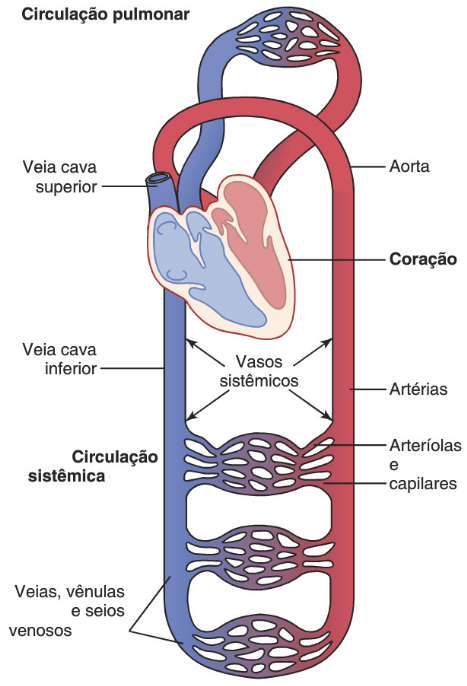
\includegraphics[scale=0.4]{figuras/revisao-sistema-circulatorio/sistema-circulatorio-humano.png}
  \fonte{Adaptado de~\cite{Hall2011}.}
  \label{fig:sistema-circulatorio}
\end{figure}

Nas ilustrações do sistema circulatório (vide Figura~\ref{fig:sistema-circulatorio}) a parte
do sangue transportada pelas artérias 
e arteríolas é representada na cor vermelha, enquanto que a parte transportada pelas veias e 
vênulas é representada na cor azul. Essa convenção vem do fato de que o sangue rico 
em oxigênio nas artérias tem uma cor vermelha mais intensa, entretanto o sangue rico em dióxido de 
carbono nas veias tem uma cor mais azulada.

O coração é basicamente uma poderosa e musculosa bomba pulsante, que mantém 
a nossa circulação ao gerar uma diferença de pressão em suas câmaras internas 
(átrio direito, ventrículo direito, átrio esquerdo e ventrículo esquerdo).

O sangue é um tecido conjuntivo formado por células (como hemácias -- glóbulos 
vermelhos -- e leucócitos -- glóbulos brancos), fragmentos de células 
(por exemplo, as plaquetas) e proteínas suspensas em uma matriz extracelular 
(o plasma, que é composto por proteínas, nutrientes, sais e hormônios).

Os vasos sanguíneos estão presentes por todo o corpo humano formando as vias de transporte nas 
quais o sangue é distribuído partindo do coração e retornando para ele. Os vasos são 
divididos em artérias, arteríolas, capilares, vênulas e veias. O sangue que é bombeado 
para fora do coração passa pelas artérias, que o transporta sob alta pressão e velocidade.
Para suportar essa alta pressão, as artérias possuem paredes vasculares mais espessas e 
rígidas do que dos demais vasos. O sangue nas artérias possui oxigênio ($O_2$) obtido durante 
a sua passagem pelos pulmões. No final da rede de artérias temos as arteríolas, que 
servem como uma espécie de ``condutos de controle'', que através de sua oclusão ou dilatação 
diminui ou aumenta (respectivamente) o fluxo sanguíneo liberado para os capilares.

Nos capilares ocorre a troca de líquidos, nutrientes, eletrólitos, hormônios e outras 
substâncias entre o sangue e o líquido intersticial. Para que essa troca possa acontecer,
as paredes dos capilares são bem finas e possuem minúsculos poros. Depois de passar 
pelos capilares, o sangue é direcionado para as vênulas que coalescem formando progressivamente
as veias. Nas veias, o sangue com o dióxido de carbono ($CO_2$) e outros restos metabólicos é 
transportado de volta para o coração. A pressão nas veias é mais baixa e suas paredes 
vasculares são mais finas e menos rígidas do que as paredes das artérias. 

Comparando a quantidade de sangue saindo do coração durante trinta minutos com a quantidade 
total de sangue no corpo humano, além de considerar o funcionamento das válvulas presentes nas veias,
o médico fisiologista William Harvey publicou em 1628 o seu livro ``\textit{De Motu Cordis et Sanguinis in Animalibus}''
com sua conclusão de que o sangue percorria um circuito circular no corpo~\cite{Whitteridge1978}.
Entretanto, Harvey não conseguiu visualizar como ocorria a passagem do sangue das partes periféricas das artérias para 
as partes periféricas das veias. Ele conjecturou que deveriam haver ``poros'' nessas regiões periféricas. Esses ``poros''
foram identificados décadas depois em 1661 por Malpighi como sendo os vasos capilares~\cite{Cliff1976}.

Atualmente sabemos que o ciclo do bombeamento do sangue começa no átrio direito (AD) do coração onde a pressão 
sanguínea é mais baixa (próxima de $0$ mmHg). Com a contração do AD o sangue é ejetado para 
o ventrículo direito (VD). Já a contração do VD ejeta o sangue para os pulmões 
(circulação pulmonar) onde o sangue receberá oxigênio e liberará dióxido de carbono. 
Dos pulmões o sangue volta para o coração entrando no átrio esquerdo (AE). Com a contração 
do AE o sangue é ejetado para o ventrículo esquerdo (VE). No VE a pressão sanguínea 
é mais alta (entre $80$ mmHg e $120$ mmHg) do que nas outras partes do coração,
sendo que com sua contração o sangue é ejetado para ser transportado para 
o resto do corpo (circulação sistêmica) através das artérias.
Depois de passar pelas arteríolas, capilares e vênulas, o sangue voltará ao coração pelas veias 
até chegar ao AD, onde o ciclo repetirá.

As artérias e veias formam estruturas que se assemelham a árvores com ramificações 
(ou bifurcações). Os trechos finais das árvores arteriais conectam-se aos trechos 
finais das árvores venosas através de vasos capilares, sendo que esses capilares 
apresentam uma estrutura que se assemelha a uma rede com diversas conexões em seus
pontos de interseção. Desse modo, temos um circuito que leva através das árvores arteriais 
o oxigênio, os nutrientes e os hormônios para os tecidos e retira através das árvores venosas 
o dióxido de carbono e os restos metabólicos.

O fluxo do sangue saindo do VE pela artéria aorta é intermitente devido ao fato do coração 
ser uma bomba pulsante. Entretanto, o fluxo do sangue chegando nos capilares é mais constante. 
Esse fenômeno foi tratado por Stephen Hales usando o efeito de Windkessel (``câmara de ar'')~\cite{Hales1733}.
Hales comparou o funcionamento do sistema composto pelas artérias e arteríolas 
com o funcionamento de um dispositivo de sua época usado no combate à incêndios. A Figura~\ref{fig:efeito-windkessel}
ilustra o conceito. Nota-se que mesmo se a água sair da bomba de modo intermitente, a água 
acumulada dentro da câmara de ar manterá algum fluxo mais constante saindo da mangueira. A artéria aorta 
possui uma complacência que permite se ajustar de modo a acumular um volume de sangue, que 
será liberado quando o coração não estiver ejetando sangue pelo VE.

\begin{figure}[!htb]
  \centering
  \captiondelim{: }
  \caption{Conceito do efeito Windkessel.} 
  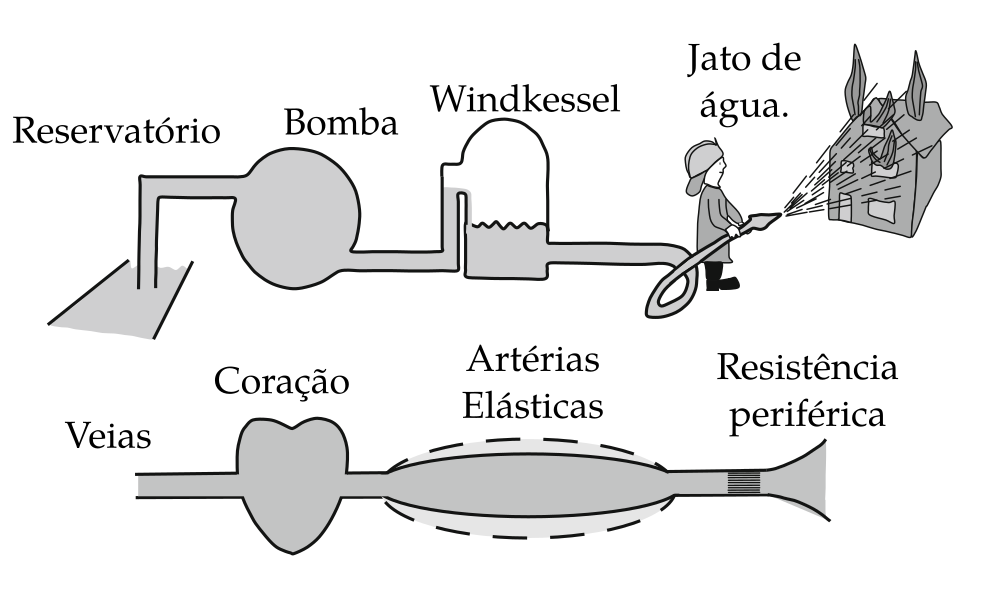
\includegraphics[scale=0.4]{figuras/revisao-sistema-circulatorio/efeito-windkessel.png}
  \fonte{Adaptado de~\cite{Westerhof2009}.}
  \label{fig:efeito-windkessel}
\end{figure}

\section{CONSTRUÇÃO DE UMA ÚNICA ÁRVORE CIRCULATÓRIA}\label{sec:cco}

Nesta seção é apresentado o método \textit{Constrained Constructive Optimization} (CCO) para 
construir uma única árvore circulatória dentro do domínio de perfusão. Este método foi inicialmente 
proposto para construir árvores vasculares 
considerando domínios bidimensionais~\cite{Schreiner1993b} e posteriormente foi
generalizado para domínios tridimensionais~\cite{Karch1999}. O método utiliza
árvores binárias adicionando sequencialmente um novo segmento com extremidade 
distal selecionada de modo aleatório no domínio de perfusão. Esse novo segmento 
é conectado a algum segmento já existente da árvore através de um ponto
de bifurcação, cuja posição é determinada de modo a minimizar uma função custo.
Durante toda a construção da árvore, condições de fluxo e pressão são levadas 
em consideração. O resultado final é uma árvore binária que possui aspectos 
morfométricos com valores próximos aos dados estatísticos de árvores vasculares 
reais encontrados na literatura especializada, 
como por exemplo o decaimento do diâmetro médio dos segmentos ao longo da árvore.
Os modelos de árvores gerados pelo método CCO utilizam às seguintes condições:

\begin{enumerate}[label=(\roman*)]
\item ramifica\c{c}\~ao binária de segmentos vasculares. Cada segmento será 
representado por um tubo rígido cilíndrico, por onde o sangue escoa em regime 
laminar e estacionário;

\item a resistência hidrodinâmica $R_i$ de um segmento $i$ é dada pela lei 
de Poiseuille~\cite{Fung1996}:
\begin{equation}
R_i = \frac{8\eta l_i}{\pi r_i^4},\label{eq:resistencia}
\end{equation}
onde $\eta$ é a viscosidade sanguínea (que será um parâmetro na simulação), 
$l_i$ e $r_i$ são, respectivamente, o comprimento e raio do segmento;

\item a queda de pressão $\Delta p_i$ ao longo do segmento $i$ é dada por:
\begin{equation}
\Delta p_i = R_i Q_i,
\label{eq:quedapressao.i}
\end{equation} 
onde $Q_i$ representa o fluxo sanguíneo através do segmento $i$;

\item a pressão $p_{term}$ na posição distal dos segmentos terminais é considerada constante;

\item $Q_{perf}$ é o fluxo sanguíneo no segmento raiz da árvore e 
$Q_{term,\,i}$ é o fluxo sanguíneo no segmento terminal $i$;

\item  a queda de pressão total $\Delta p$ da árvore é dada por 
\begin{equation}
  \Delta p = p_{perf} - p_{term},\label{eq:quedapressao}
\end{equation}
onde $p_{perf}$ é a pressão de perfusão na posi\c{c}\~ao proximal do segmento raiz;

\item em cada bifurcação, o raio do segmento pai ($r$) e dos segmentos filhos à esquerda ($r_{left}$) e 
à direita ($r_{right}$) obedecem uma lei de potência expressa por~\cite{Sherman1981}:
\begin{equation}
r^{\gamma} = r_{left}^{\gamma} + r_{right}^{\gamma},\label{eq:leibifurcacao}
\end{equation}
onde $\gamma$ é um valor pré-estabelecido no início da simulação do algoritmo CCO.

\item os segmentos são gerados de modo a minimizar a função custo (volume total da árvore)
expressa por:
\begin{equation}
  T = \pi \sum_{i=1}^{K_{tot}} l_i r_i^2,
  \label{eq:volume}
\end{equation}
onde $K_{tot}$ é o número de segmentos na árvore em cada iteração do algoritmo.
\end{enumerate}

\subsection{Critério de distância mínima}\label{sec:criterio-distancia-minima}

O Algoritmo~\ref{algo:CCOclassico} descreve a construção de uma árvore vascular pelo método CCO. 
Inicialmente o ponto proximal $\mathbf{x}_{root}$ do segmento raiz é conectado a um 
ponto $\mathbf{x}_{inew}$ escolhido de modo aleatório no domínio de perfusão $D_{perf}$.
As coordenadas desse ponto são números pseudoaleatórios seguindo uma distribuição uniforme.
Em seguida, começa um processo iterativo com $N_{term}-1$ passos. Para cada passo um novo 
ponto $\mathbf{x}_{inew}$ é gerado aleatoriamente e validado. Para validar 
esse ponto é verificado se ele está no interior do domínio de perfusão e se ele 
está a uma distância mínima $d_{min}$ de todos os segmentos criados nos passos 
anteriores (vide Figura~\ref{fig:criterio-distancia-critica}).
O valor de $d_{min}$ é diminuído a medida que o número de segmentos terminais aumenta.
Caso $\mathbf{x}_{inew}$ não passe pela validação, uma nova posição é gerada. Se esse 
ponto for gerado $N_{toss}$ vezes sem conseguir passar pela validação, então o valor de
$d_{min}$ é atualizado como $\beta d_{min}$, onde $\beta \in (0,\,1)$ é um fator
constante de redução. Para calcular a distância entre $\mathbf{x}_{inew}$ e um segmento
$\overline{AB}$, utiliza-se a distância crítica definida por
\begin{equation}
 \dist_{crit}(\mathbf{x}_{inew}, \overline{AB}) = \begin{cases}
                \dfrac{\left\|\overrightarrow{A\mathbf{x}_{inew}} \times \overrightarrow{AB}\right\|}{\left\|\overrightarrow{AB}\right\|}
                \textrm{, se }0 \leq \dfrac{\overrightarrow{A\mathbf{x}_{inew}}\cdot \overrightarrow{AB}}{\overrightarrow{AB}\cdot \overrightarrow{AB}} \leq 1;\\
                \min\{\dist(A,\,\mathbf{x}_{inew}),\, \dist(B,\,\mathbf{x}_{inew}) \}\textrm{, caso contrário;}
               \end{cases}
 \label{eq:dist-critica}
\end{equation}
onde $\dist(P,\,Q)$ representa a distância Euclidiana entre os pontos $P$ e $Q$ e 
$\min\{a,\,b\}$ representa o mínimo entre os números reais $a$ e $b$. Nota-se
que quando ocorre o caso 
$0\leq \dfrac{\overrightarrow{A\mathbf{x}_{inew}}\cdot \overrightarrow{AB}}{\overrightarrow{AB}\cdot \overrightarrow{AB}} \leq 1$ 
isso significa que pode ser traçada uma reta passando no ponto $\mathbf{x}_{inew}$
e interceptando o segmento $\overline{AB}$, de modo que essa reta seja perpendicular à $\overline{AB}$. Por isso,
nesse caso, calcula-se a distância crítica usando a
expressão $\dfrac{\left\|\overrightarrow{A\mathbf{x}_{inew}} \times \overrightarrow{AB}\right\|}{\left\|\overrightarrow{AB}\right\|}$,
que coincide com a fórmula para calcular a distância entre um ponto $\mathbf{x}_{inew}$ e a reta
passando por $A$ e $B$.

\begin{figure}[!htb]
  \centering
  \captiondelim{: }
  \caption{Ponto $\mathbf{x}_{inew}$ obedecendo à uma distância mínima $d_{min}$ em relação aos segmentos da árvore.}
  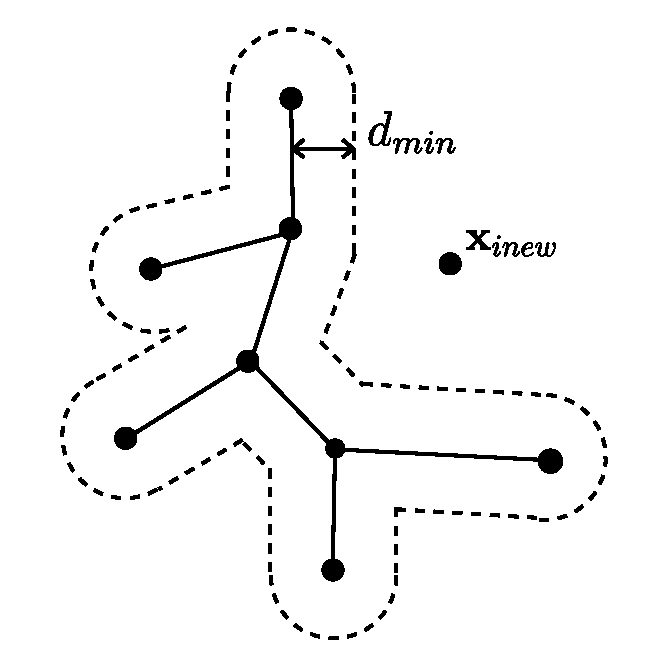
\includegraphics[scale=0.5]{figuras/modelos-computacionais-de-arvores-circulatorias/criterio-distancia-critica.pdf}
  \fonteAutor{2022}
  \label{fig:criterio-distancia-critica}
\end{figure}


\begin{algorithm}
\Dados{$D_{perf}$, $\mathbf{x}_{root}$, $Q_{perf}$, $N_{term}$, $\Delta p$, $\gamma$, $N_{con}$, $\eta$.}
  Gerar e validar uma posi\c{c}\~ao distal $\mathbf{x}_{inew}$ do segmento raiz\;
  Conectar $\mathbf{x}_{inew}$ a $\mathbf{x}_{root}$ (\textit{plantar o segmento raiz da árvore})\;
  \For{($i\gets 1$ \KwTo $N_{term}$)}{
    Gerar e validar a posi\c{c}\~ao distal $\mathbf{x}_{inew}$ de um novo segmento terminal\;
    Determinar $N \leq N_{con}$ segmentos na árvore que estão mais próximos de $\mathbf{x}_{inew}$\;
    \For{($j\gets 0$ \KwTo N)}{
      Conectar $\mathbf{x}_{inew}$ temporariamente no segmento $j$, 
      criando a bifurca\c{c}\~ao $\mathbf{x}_{ibif}$\;
      Otimizar e validar a posi\c{c}\~ao de $\mathbf{x}_{ibif}$\;
      Armazenar resultados de $\mathbf{x}_{ibif}$ na Tabela de Avaliação de Conexões (TAC)\;
      Descartar conexão temporária $\mathbf{x}_{ibif}$\;
    }
    Obter a Tabela de Avaliação de Conexões Reduzida (TAC$_r$) a partir de TAC removendo as conexões inválidas\;
    Determinar em TAC$_r$ a bifurcação ótima $\mathbf{x}_{iopt}$\;
    Conectar $\mathbf{x}_{inew}$ a $\mathbf{x}_{iopt}$ de modo permanente\;
  }
\caption{Gera\c{c}ão de árvore arterial pelo método CCO.}
\label{algo:CCOclassico}
\end{algorithm}

\subsection{Ajuste dos raios dos segmentos}\label{sec:ajuste-dos-raios}

Depois que $\mathbf{x}_{inew}$ é gerado e validado, são determinados $N \leq N_{con}$ 
segmentos da árvore que estão mais próximos dele. O valor de $N_{con}$ é fixo e fornecido 
como entrada do algoritmo. Em~\cite{Karch1999}, $N_{con} = 20$ é obtido como sendo adequado para 
encontrar a otimização local da função custo. Para cada um dos $N$ segmentos encontrados, 
uma nova árvore pode ser formada temporariamente conectando $\mathbf{x}_{inew}$ 
em um ponto do segmento encontrado. Cada bifurcação $\mathbf{x}_{ibif}$ é formada 
pelos segmentos $ibif$ (segmento de bifurcação), $icon$ (segmento de conexão)
e $inew$ (novo segmento), conforme ilustra a Figura~\ref{fig:passos-cco}. 
Inicialmente $\mathbf{x}_{ibif}$ é escolhido como o ponto médio do segmento. 
O segmento $inew$ adiciona um fluxo $Q_{inew}$ na árvore e isso 
perturba o fluxo $Q_{term,\,i}$ que os segmentos terminais devem ter. Para corrigir 
isso deve-se ajustar a resistência hidrodinâmica da árvore. Considerando que o comprimento 
dos segmentos não se altera e que as pressões de perfusão e terminal são fixas, 
efetua-se esse ajuste através da alteração dos raios dos segmentos 
criados na conexão temporária. Entretanto, ao invés de calcular diretamente 
esses raios, é efetuado o cálculo das razões entre o raio do segmento pai $ibif$ 
e seus filhos $icon$ e $inew$.

\begin{figure}[!htb]
  \centering
  \captiondelim{: }
  \caption{Ilustração dos passos básicos do Algoritmo~\ref{algo:CCOclassico}.
    (a) O ponto $\mathbf{x}_{inew}$ é escolhido aleatoriamente dentro do domínio de perfusão
    e testado para verificar o critério de distância mínima. Caso não atenda ao critério, outro
    ponto deve ser escolhido.
    (b) Conecta-se o ponto $\mathbf{x}_{inew}$ aos segmentos mais próximos na árvore. 
    Cada conexão cria um ponto $\mathbf{x}_{ibif}$.
    (c) Desloca-se a conexão $\mathbf{x}_{ibif}$ de modo a minimizar a função custo.
    }
  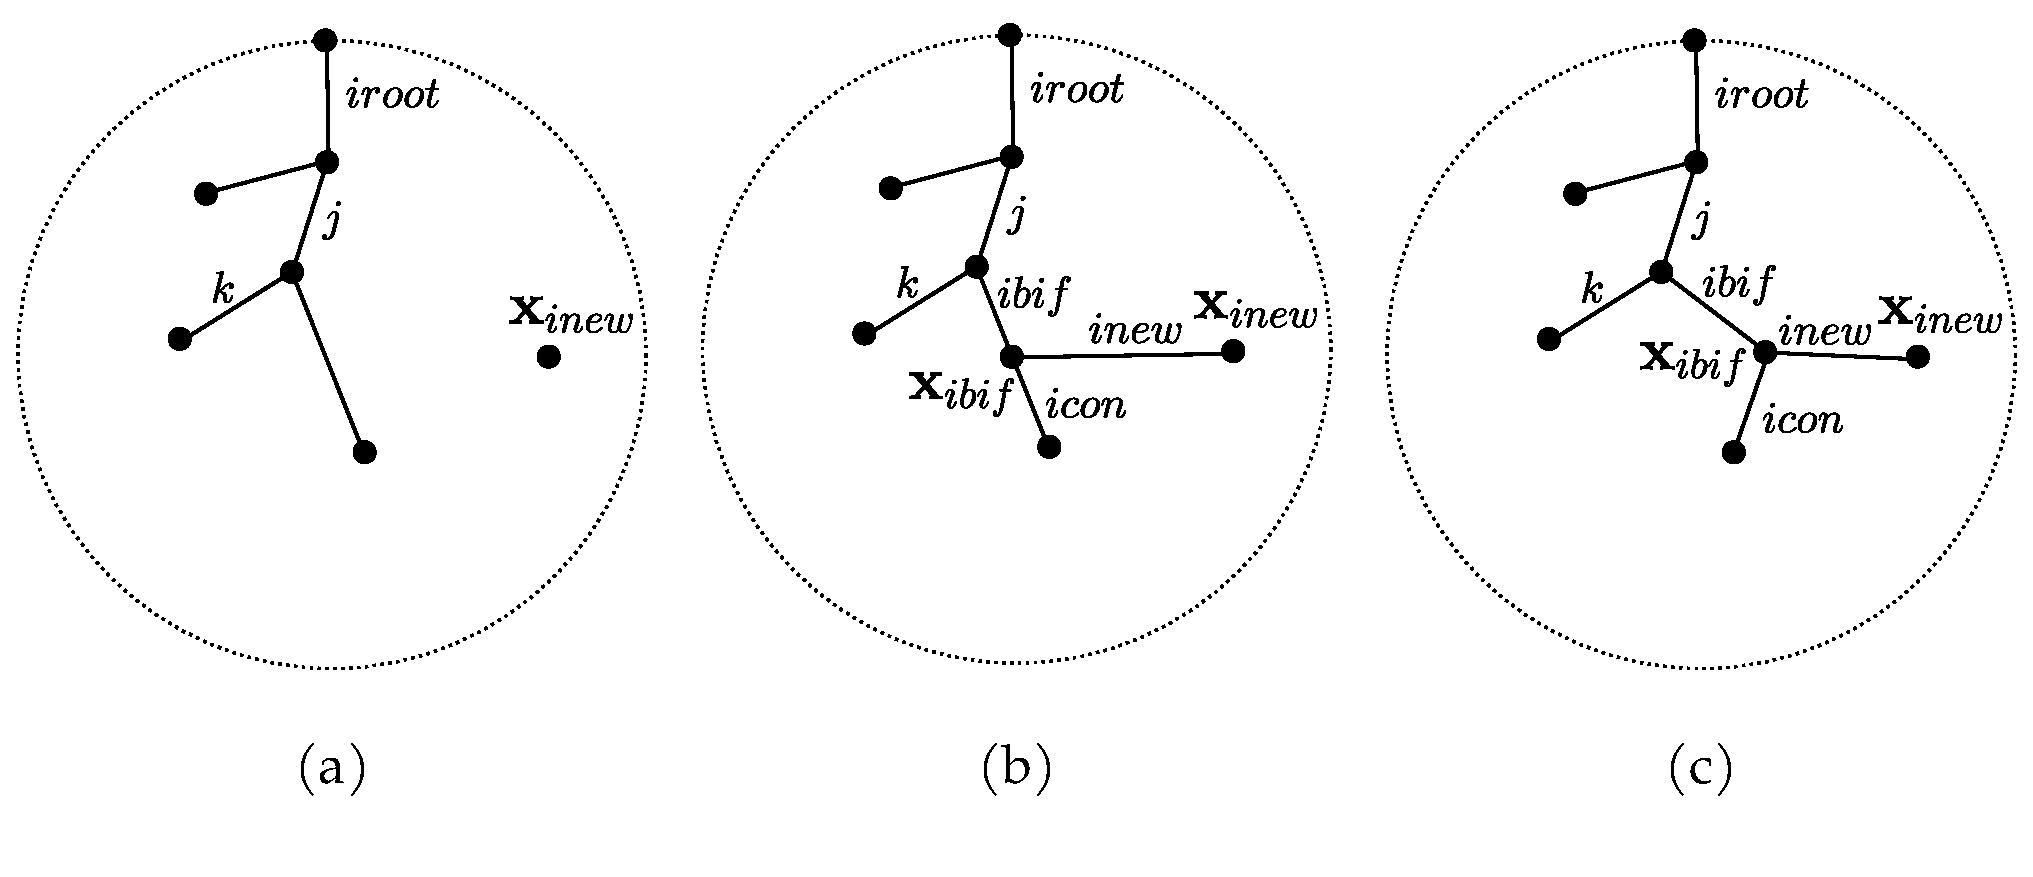
\includegraphics[scale=0.4]{figuras/modelos-computacionais-de-arvores-circulatorias/passos-algoritmo-cco.eps}
  \fonteAutor{2022}
  \label{fig:passos-cco}
\end{figure}

Como a pressão terminal é considerada constante, usando a equação~\eqref{eq:quedapressao.i} 
a razão do fluxo se dividindo no segmento $ibif$ será dada por
\begin{equation}
  R_{sub,\,icon}Q_{icon} = R_{inew}Q_{inew} \iff \frac{Q_{icon}}{Q_{inew}} = \frac{R_{inew}}{R_{sub,\,icon}}
  \iff \frac{Q_{icon}}{Q_{inew}} = \frac{\dfrac{R^*_{inew}}{r^4_{inew}}}{\dfrac{R^*_{sub,\,icon}}{r^4_{icon}}},
  \label{eq:razao.fluxo}
\end{equation}
onde $R_{sub,\,icon}$ é a resistência do segmento $icon$ incluindo suas subárvores 
esquerda e direita, $R_{inew}$ é a resistência do segmento $inew$, $R^*_{inew} = R_{inew}r^4_{inew}$
e $R^*_{sub,\,icon} = R_{sub,\,icon}r^4_{icon}$ são definidos como as resistências
reduzidas. Da equação~\eqref{eq:resistencia}, obtém-se diretamente 
$R^*_{inew} = \frac{8\eta l_{inew}}{\pi}$. Para obter $R^*_{sub,\,icon}$, devem ser 
consideradas as regras de cálculo de resistência de tubos conectados em série e em 
paralelo. Por exemplo, a resistência reduzida $R^*_{sub,\,j}$ de um segmento $j$ 
incluindo suas subárvores esquerda e direita será dada por
\begin{eqnarray}
  R^*_{sub,\,j} &=& \left[R_{j} + \left(\dfrac{1}{R_{left,\,j}} + \dfrac{1}{R_{right,\,j}}\right)^{-1}\right]r^4_j \nonumber\\ 
  &=& \frac{8\eta l_{j}}{\pi} + \left(\dfrac{r^{-4}_j}{R_{left,\,j}} + \dfrac{r^{-4}_j}{R_{right,\,j}}\right)^{-1} \nonumber\\
  &=& \frac{8\eta l_{j}}{\pi} + \left(\dfrac{r^4_{left,\,j}r^{-4}_j}{R^*_{left,\,j}} + \dfrac{r^4_{right,\,j}r^{-4}_j}{R^*_{right,\,j}}\right)^{-1} \nonumber\\
  &=& \frac{8\eta l_{j}}{\pi} + \left[\dfrac{\left(\frac{r_{left,\,j}}{r_j}\right)^4}{R^*_{left,\,j}} + \dfrac{\left(\frac{r_{right,\,j}}{r_j}\right)^4}{R^*_{right,\,j}}\right]^{-1}.
  \label{eq:resistencia.reduzida}
\end{eqnarray}

Em~\eqref{eq:resistencia.reduzida}, $R^*_{left,\,j}$ é a resistência reduzida da 
subárvore esquerda do segmento $j$ e $r_{left,\,j}$ é o raio de entrada dessa subárvore. 
De modo análogo, $R^*_{right,\,j}$ e $r_{right,\,j}$ são referentes à subárvore direita. 
Aplicando~\eqref{eq:resistencia.reduzida}, calcula-se $R^*_{sub,\,icon}$ de modo recursivo.

Isolando os raios em~\eqref{eq:razao.fluxo}, obtém-se a razão entre os raios dos 
segmentos filhos de $ibif$:
\begin{equation}
  \dfrac{r_{icon}}{r_{inew}} = \sqrt[4]{\frac{Q_{icon}R^*_{sub,\,icon}}{Q_{inew}R^*_{inew}}}.
  \label{eq:razao.raios}
\end{equation}

Por outro lado, usando~\eqref{eq:leibifurcacao} obtém-se as ``razões de bifurcação''
em relação a $ibif$:
\begin{eqnarray}
  \beta_{ibif}^{icon} &=& \dfrac{r_{icon}}{r_{ibif}} = \left[1 + \left(\dfrac{r_{icon}}{r_{inew}}\right)^{-\gamma}\right]^{-\frac{1}{\gamma}}, \label{eq:razao.bifurcacao.ibif.icon} \\ 
  & & \nonumber\\
  \beta_{ibif}^{inew} &=& \dfrac{r_{inew}}{r_{ibif}} = \left[1 + \left(\dfrac{r_{icon}}{r_{inew}}\right)^{\gamma}\right]^{-\frac{1}{\gamma}}. \label{eq:razao.bifurcacao.ibif.inew}
\end{eqnarray}

Os valores $\beta_{ibif}^{icon}$ e $\beta_{ibif}^{inew}$ são determinados 
unicamente pela razão do fluxo se dividindo em $ibif$ dada por $\frac{Q_{icon}}{Q_{inew}}$
e pela geometria da árvore através da razão $\frac{R^*_{sub,\,icon}}{R^*_{inew}}$.
Entretanto, o novo fluxo saindo por $inew$ precisa antes passar por 
$ibif$. Considerando $ibif$ e $k$ como os filhos do segmento $j$, será 
necessário então calcular as razões de bifurcação $\beta_{j}^{ibif}$ e $\beta_{j}^{k}$.
Continuando esse raciocínio, devem ser calculadas todas as razões de bifurcação dos 
segmentos no único caminho subindo a árvore a partir de $ibif$ até o segmento 
raiz ($iroot$). Nesse procedimento apenas as razões de bifurcação são armazenadas, 
não havendo necessidade de armazenar o valor dos raios dos segmentos. 
Quando for necessário o valor do raio do segmento $j$, ele pode ser obtido por
\begin{equation}
 r_j = r_{iroot} \prod_{k \in \textrm{path}(j, iroot)} \beta_{k},
 \label{eq:raio.segmento.j}
\end{equation}
onde $\beta_{k}$ é a razão de bifurcação entre o segmento $k$ e seu respectivo pai e 
$\textrm{path}(j, iroot)$ é o único caminho subindo a árvore a partir de $j$ até 
o segmento raiz ($iroot$). O valor de $r_{iroot}$ é obtido por
\begin{equation}
 r_{iroot} = \sqrt[4]{\dfrac{R^{*}_{sub,iroot}}{R_{sub,iroot}}} = \sqrt[4]{R^{*}_{sub,iroot}\dfrac{Q_{perf}}{\Delta p}},
 \label{eq:raio.iroot}
\end{equation}
onde $\Delta p = p_{perf} - p_{term}$ e $R_{sub,iroot}$ acaba denotando a resistência hidrodinâmica total da árvore.

Até aqui foram determinadas $N$ árvores temporárias, cada uma com seus valores 
para $\mathbf{x}_{ibif}$ e suas atualizações da razão das bifurcações. A posição de 
cada $\mathbf{x}_{ibif}$ será ainda otimizada de modo a minimizar a função custo 
dada por~\eqref{eq:volume}.

\subsection{Otimização geométrica}\label{sec:otimizacao-geometrica}

A nova posição de $\mathbf{x}_{ibif}$ será localizada
através de busca exaustiva dentro da região interna do triângulo 
formado pelos três pontos nos segmentos $ibif$, $inew$ e $icon$ que são distintos de $\mathbf{x}_{ibif}$.
Esse triângulo está contido no chamado plano de bifurcação~\cite{Karch1999}. 
Considera-se um mapeamento do triângulo de referência formado por $P_{i} = (0,\,0)$, 
$P_{j} = (1,\,0)$ e $P_{inew} = (0,\,1)$ com o triângulo formado pelos pontos 
$\mathbf{x}_{i}$, $\mathbf{x}_{j}$ e $\mathbf{x}_{inew}$ conforme ilustrado na 
Figura~\ref{fig:otimizacao-ponto-bifurcacao}. O mapeamento 
$\mathrm{map}:\mathbb{R}^2\to\mathbb{R}^3$ é definido tal que $\mathrm{map}(P_i) = \mathbf{x}_{i}$, 
$\mathrm{map}(P_j) = \mathbf{x}_{j}$ e $\mathrm{map}(P_{inew}) = \mathbf{x}_{inew}$. 
Esse mapeamento pode ser dado por:
\begin{equation}
  \mathrm{map}(a,\,b) = (1 - a - b)\mathbf{x}_{i} + a\mathbf{x}_{j} + b\mathbf{x}_{inew}
  \label{eq:mapeamento-bifucacao}
\end{equation}

Considere então os pontos $P_{ibif} = \left(\dfrac{m}{n},\,\dfrac{k}{n}\right)$, com $n > 1$ um 
número natural, $k = 0$, 1, 2,\ldots, $n$ e $m = 0$, 1, \ldots, $(n-k)$. A função custo~\eqref{eq:volume} 
será avaliada considerando $\mathbf{x}_{ibif} = \mathrm{map}(P_{ibif})$ e o menor valor será 
armazenado. Nas simulações realizadas neste trabalho, adotou-se $n = 5$ para tentar reduzir o 
custo computacional nesta etapa de otimização do algoritmo. Nota-se que isso significa dividir cada 
lado do triângulo de referência em cinco partes iguais.

\begin{figure}[!htb]
  \centering
  \captiondelim{: }
  \caption{Mapeamento para localizar a posição ótima de $\mathbf{x}_{ibif}$ que minimiza a função custo~\eqref{eq:volume}.}
  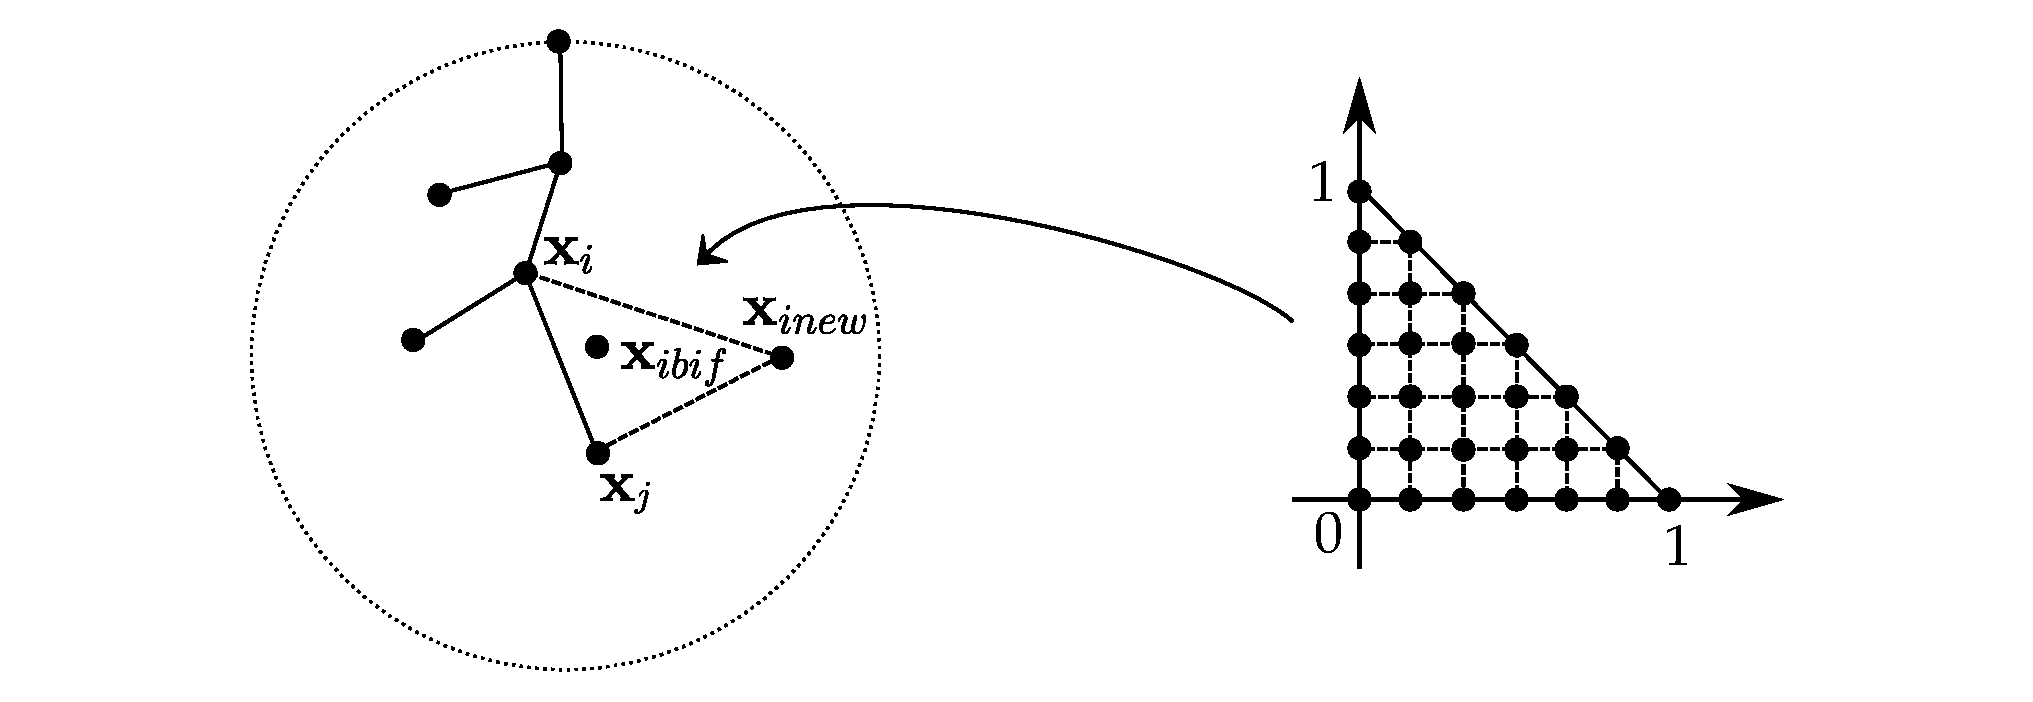
\includegraphics[width=\textwidth]{figuras/modelos-computacionais-de-arvores-circulatorias/otimizacao-do-ponto-de-bifurcacao.eps}
  \fonteAutor{2022}
  \label{fig:otimizacao-ponto-bifurcacao}
\end{figure}

A posição encontrada será válida se $\mathbf{x}_{ibif}$ permanecer no domínio de perfusão e 
os comprimentos dos segmentos $ibif$, $inew$ e $icon$ forem maiores do que seus respectivos 
diâmetros.

\subsection{Otimização estrutural}\label{sec:otimizacao-estrutural}

Como a posição de $\mathbf{x}_{ibif}$
será alterada, isso implica em alterar o comprimento de $ibif$, $inew$ e $icon$ e consequentemente
a resistência hidrodinâmica da árvore. Desse modo, devem ser atualizadas as razões de bifurcação 
desde esses segmentos até a raiz da árvore. Os resultados de cada árvore temporária serão armazenados 
na Tabela de Avaliação de Conexão (TAC). A TAC será posteriormente reduzida para TAC$_r$, na qual as 
conexões inválidas serão removidas (isto é, remover os casos onde o $inew$ intercepte algum segmento 
existente na árvore). Caso TAC$_r$ seja vazia, um novo ponto $\mathbf{x}_{inew}$ deve ser 
escolhido e as iterações são reiniciadas. Caso contrário, em TAC$_r$ é determinada a bifurcação 
ótima $\mathbf{x}_{iopt}$, ou seja, que gera o menor valor para a função custo. A bifurcação 
$\mathbf{x}_{iopt}$ é conectada a $\mathbf{x}_{inew}$ de modo permanente. Desse modo, a árvore 
passa a ter um segmento terminal a mais e o algoritmo vai reiniciar suas iterações até que seja 
atingido a quantidade $N_{term}$ de terminais.

\subsection{Interseção entre segmentos}\label{sec:intersecao-entre-segmentos}

Durante o processo de otimização geométrica (conforme descrito na Seção~\ref{sec:otimizacao-geometrica}) são 
alterados os segmentos $s_c$ e seus filhos $s_{i-1}$ e $s_{i}$ (onde $s_{i-1}$ é o segmento de conexão referente 
ao segmento terminal $s_i$). Eventualmente essa alteração pode fazer com que $s_c$, $s_{i-1}$ ou $s_i$ 
intercepte algum outro segmento da árvore. Caso ocorra alguma interseção, isso deve ser identificado 
durante a redução da Tabela de Avaliação de Conexões (conforme descrito na Seção~\ref{sec:otimizacao-estrutural}).
Para determinar se existe interseção entre o segmento $s_u$ (com $u=c$, $u=i-1$ ou $u=i$) e um outro segmento 
$s_v$ da árvore, considera-se dois casos distintos conforme esteja-se trabalhando com pontos em $\mathbb{R}^2$ ou 
com pontos em $\mathbb{R}^3$.

\subsubsection{Segmentos no $\mathbb{R}^2$}\label{subsec:intersecao-2d}

Suponha que os pontos proximal e distal do segmento $s_u$ sejam, respectivamente, 
$A = (x_A,\, y_A)$ e $B = (x_B,\, y_B)$. 
Por outro lado, suponha que os pontos proximal e distal do segmento $s_v$ sejam, respectivamente, 
$C = (x_C,\, y_C)$ e $D = (x_D,\, y_D)$. 
As retas suporte $u$ e $v$, respectivamente, de $s_u$ e $s_v$ são dadas por:
\begin{eqnarray}
  u: & X = A + \lambda_u\overrightarrow{AB}\label{eq:reta-suporte-do-segmento-su}, \\
  v: & X = C + \lambda_v\overrightarrow{CD}\label{eq:reta-supor	te-do-segmento-sv}.
\end{eqnarray}

Nota-se que os pontos de $s_u$ e $s_v$ são tais que, respectivamente, 
tem-se $\lambda_u\in[0, 1]$ e $\lambda_v\in[0, 1]$. Além disso, a interseção entre 
as retas $u$ e $v$ ocorre quando:
\begin{equation}
  A + \lambda_u\overrightarrow{AB} = C + \lambda_v\overrightarrow{CD}.
  \label{eq:intersecao-segmentos-caso-2d}
\end{equation}

A solução dessa equação será dada por:
\begin{equation}
  \begin{cases}
    \lambda_u = \dfrac{(x_D - x_C)(y_C - y_A) - (x_C - x_A)(y_D - y_C)}{(x_D - x_C)(y_B - y_A) - (x_B - x_A)(y_D - y_C)}\\ \\
    \lambda_v = \dfrac{(x_B - x_A)(y_C - y_A) - (x_C - x_A)(y_B - y_A)}{(x_D - x_C)(y_B - y_A) - (x_B - x_A)(y_D - y_C)}
  \end{cases}
  \label{eq:solucao-sistema-intersecao-segmentos-caso-2d}
\end{equation}

Quando as retas $u$ e $v$ são paralelas não há interseção e portanto esse sistema não tem solução.
Considera-se que esse seja o caso quando
\begin{equation}
  |(x_D - x_C)(y_B - y_A) - (x_B - x_A)(y_D - y_C)| < \varepsilon,
  \label{eq:solucao-tolerancia-sistema-intersecao-segmentos-caso-2d}
\end{equation}
onde $\varepsilon = 10^{-12}$ é uma tolerância.

Por outro lado, quando $u$ e $v$ não são paralelas, elas se interceptam e o sistema tem solução.
Considera-se que a interseção ocorre sobre $s_u$ e $s_v$ quando: 
\begin{equation}
  \begin{cases}
    0 < \lambda_u < 1 + \dfrac{r_u + r_v}{\left\|\overrightarrow{AB}\right\|} \\
    \\
    0 < \lambda_v < 1 + \dfrac{r_u + r_v}{\left\|\overrightarrow{CD}\right\|}
  \end{cases},
  \label{eq:solucao-tolerancia-intersecao-segmentos-caso-2d}
\end{equation}
onde $r_u$ e $r_v$ são, respectivamente, os raios de $s_u$ e $s_v$.

\subsubsection{Segmentos no $\mathbb{R}^3$}\label{subsec:intersecao-3d}

Suponha que os pontos proximal e distal do segmento $s_u$ sejam, respectivamente, 
$A = (x_A,\, y_A,\, z_A)$ e $B = (x_B,\, y_B,\, z_B)$. 
Por outro lado, suponha que os pontos proximal e distal do segmento $s_v$ sejam, respectivamente, 
$C = (x_C,\, y_C,\, z_C)$ e $D = (x_D,\, y_D,\, z_D)$. Além disso, 
sejam $P = (x_P, y_P, z_P)$ um ponto sobre $s_u$ e 
$Q = (x_Q, y_Q, z_Q)$ um ponto sobre $s_v$. As retas suporte $u$ e $v$, 
respectivamente, de $s_u$ e $s_v$ são dadas por:
\begin{eqnarray}
  u: & X = A + \lambda_u\overrightarrow{AB}\label{eq:reta-suporte-do-segmento-su-3d}, \\
  v: & X = C + \lambda_v\overrightarrow{CD}\label{eq:reta-suporte-do-segmento-sv-3d}.
\end{eqnarray}

Se o vetor $\overrightarrow{PQ}$ for ortogonal ao mesmo tempo à $s_u$ e $s_v$, então seu módulo
será o menor possível. Nesse caso, tem-se o sistema de equações:
\begin{equation}
  \begin{cases}
    P = A + \lambda_u\overrightarrow{AB}\\
    Q = C + \lambda_v\overrightarrow{CD}\\
    \langle \overrightarrow{PQ}, \, \overrightarrow{AB}\rangle = 0\\
    \langle \overrightarrow{PQ}, \, \overrightarrow{CD}\rangle = 0\\
  \end{cases}
  \label{eq:intersecao-segmentos-caso-3d}
\end{equation}
 
Nota-se que $P$ e $Q$ são tais que, respectivamente, 
tem-se $\lambda_u\in[0, 1]$ e $\lambda_v\in[0, 1]$. Reescrevendo~\eqref{eq:intersecao-segmentos-caso-3d} de forma mais
conveniente, obtém-se que:
\begin{equation}
  % <AB, AB>*r - <AB, CD>*s = <AC, AB>
  % <AB, CD>*r - <CD, CD>*s = <AC, CD>
  \begin{cases}
    \langle \overrightarrow{AB}, \, \overrightarrow{AB}\rangle \lambda_u - \langle \overrightarrow{AB}, \, \overrightarrow{CD}\rangle\lambda_v = \langle \overrightarrow{AC}, \, \overrightarrow{AB}\rangle \\
    \langle \overrightarrow{AB}, \, \overrightarrow{CD}\rangle \lambda_u - \langle \overrightarrow{CD}, \, \overrightarrow{CD}\rangle\lambda_v = \langle \overrightarrow{AC}, \, \overrightarrow{CD}\rangle
  \end{cases}.
  \label{eq:sistema-intersecao-segmentos-caso-3d}
\end{equation}

A solução desse sistema será dada por:
\begin{equation}
  \begin{cases}
    \lambda_u = \dfrac{\langle \overrightarrow{AB}, \, \overrightarrow{CD}\rangle \langle \overrightarrow{AC}, \, \overrightarrow{CD}\rangle - \langle \overrightarrow{AC}, \, \overrightarrow{AC}\rangle \langle \overrightarrow{CD}, \, \overrightarrow{CD}\rangle}{\langle \overrightarrow{AB}, \, \overrightarrow{CD}\rangle ^2 - \langle \overrightarrow{AB}, \, \overrightarrow{AB}\rangle \langle \overrightarrow{CD}, \, \overrightarrow{CD}\rangle}\\ \\
    \lambda_v = \dfrac{\langle \overrightarrow{AB}, \, \overrightarrow{AB}\rangle \langle \overrightarrow{AC}, \, \overrightarrow{CD}\rangle - \langle \overrightarrow{AC}, \, \overrightarrow{AB}\rangle \langle \overrightarrow{AB}, \, \overrightarrow{CD}\rangle}{\langle \overrightarrow{AB}, \, \overrightarrow{CD}\rangle ^2 - \langle \overrightarrow{AB}, \, \overrightarrow{AB}\rangle \langle \overrightarrow{CD}, \, \overrightarrow{CD}\rangle}
  \end{cases}
  \label{eq:solucao-sistema-intersecao-segmentos-caso-3d}
\end{equation}

Quando as retas $u$ e $v$ são paralelas existem infinitos vetores $\overrightarrow{PQ}$ 
que atendem ao sistema~\eqref{eq:sistema-intersecao-segmentos-caso-3d} e portanto ele
possui infinitas soluções. Considera-se que esse seja o caso quando
\begin{equation}
  \left|\langle \overrightarrow{AB}, \, \overrightarrow{CD}\rangle ^2 - \langle \overrightarrow{AB}, \, \overrightarrow{AB}\rangle \langle \overrightarrow{CD}, \, \overrightarrow{CD}\rangle\right| < \varepsilon,
  \label{eq:solucao-tolerancia-sistema-intersecao-segmentos-caso-3d}
\end{equation}
onde $\varepsilon = 10^{-6}$ é uma tolerância.

Por outro lado, quando $u$ e $v$ não são paralelas existe um único vetor $\overrightarrow{PQ}$ 
que atende ao sistema~\eqref{eq:sistema-intersecao-segmentos-caso-3d} e portanto ele
possui uma única solução. Considera-se que haverá interseção sobre $s_u$ e $s_v$ quando: 
\begin{equation}
  \begin{cases}
    0 < \lambda_u < 1 \\
    0 < \lambda_v < 1 \\
	\left\|\overrightarrow{PQ}\right\| < r_u + r_v
  \end{cases},
  \label{eq:solucao-tolerancia-intersecao-segmentos-caso-3d}
\end{equation}
onde $r_u$ e $r_v$ são, respectivamente, os raios de $s_u$ e $s_v$.

\section{CONSTRUÇÃO DE MÚLTIPLAS ÁRVORES ARTERIAIS}\label{sec:construcao-de-multiplas-arvores}

O método CCO~\cite{Karch1999,Schreiner1993b} cria apenas uma árvore vascular por vez.
Entretanto, em geral encontra-se mais de uma árvore presente nos tecidos e órgãos. 
A partir de artérias fonte surgem as artérias perfurantes, sendo que a partir dessas,
continuando a vascularização, podemos ter outras árvores vasculares dentro de um 
mesmo domínio de perfusão. Essas árvores podem competir entre si na distribuição do fluxo sanguíneo.
Além disso, podemos encontrar árvores de tipos diferentes (por exemplo, 
uma arterial e outra venosa).

Para a construção de múltiplas árvores em um mesmo domínio de perfusão 
podemos adotar duas estratégias básicas. Uma primeira estratégia pode ser 
subdividir o domínio de perfusão em subdomínios e aplicar o método CCO 
em cada um deles para construir sua respectiva árvore.
Em~\cite{Blanco2013}, um método variacional é utilizado para efetuar essa subdivisão
do domínio.

Por outro lado, uma segunda estratégia envolve alterar o próprio método
CCO de modo a criar mais de uma árvore simultaneamente sem subdividir o domínio de
perfusão. Em~\cite{Queiroz2018}, o método CCO foi adaptado para construir
duas ou mais árvores de modo a ter seus segmentos terminais conectados em 
seus pontos distais. Essa conexão representa a escala da microcirculação, na qual encontramos a 
rede de vasos capilares. As árvores criadas não competem entre si pelo fluxo
sanguíneo durante a construção da floresta. 
Já em~\cite{Jaquet2019} o método CCO foi alterado para construir as árvores 
de modo a alcançar um determinado percentual do fluxo sanguíneo total, sendo que as árvores
competem pelo fluxo durante a construção. Diferente da proposta em~\cite{Queiroz2018}, 
essas árvores não apresentam uma conexão nos pontos distais de seus segmentos terminais.

\subsection{Construção de árvores arteriais e venosas acopladas}\label{subsec:arvores-arterial-venosa}

Suponha que o modelo geométrico de um sistema vascular arteriovenoso seja formado por 
duas ou mais árvores circulatórias conectadas em seus segmentos vasculares terminais. Para a construção 
deste modelo, utilizou-se o Algoritmo~\ref{algo:CCOVenosoArterial} baseado no método CCO~\cite{Queiroz2018}.
As árvores deste modelo atendem as mesmas condições do CCO descritas na Seção~\ref{sec:cco}. A 
Figura~\ref{fig:CCOVenosoArterial} ilustra os passos do Algoritmo~\ref{algo:CCOVenosoArterial} 
para construir um modelo com duas árvores vasculares ($N_{trees} = 2$), cada uma com 
dois segmentos terminais ($N_{term} = 2$).

\begin{figure}[!htb]
  \centering
  \captiondelim{: }
  \caption{Representa\c{c}\~ao da gera\c{c}\~ao de um sistema vascular arteriovenoso. 
  A cor azul representa a árvore venosa e a vermelha a árvore arterial.
  (a) Conexão de $\mathbf{x}_{inew}$ com $\mathbf{x}_{prox}^1$ e $\mathbf{x}_{prox}^2$.
  (b) Conexão de $\mathbf{x}_{inew}$ com $\mathbf{x}_{ibif}^1$ e $\mathbf{x}_{ibif}^2$.
  (c) Deslocamento de $\mathbf{x}_{ibif}^1$ e $\mathbf{x}_{ibif}^2$ de modo a otimizar a função custo.}
  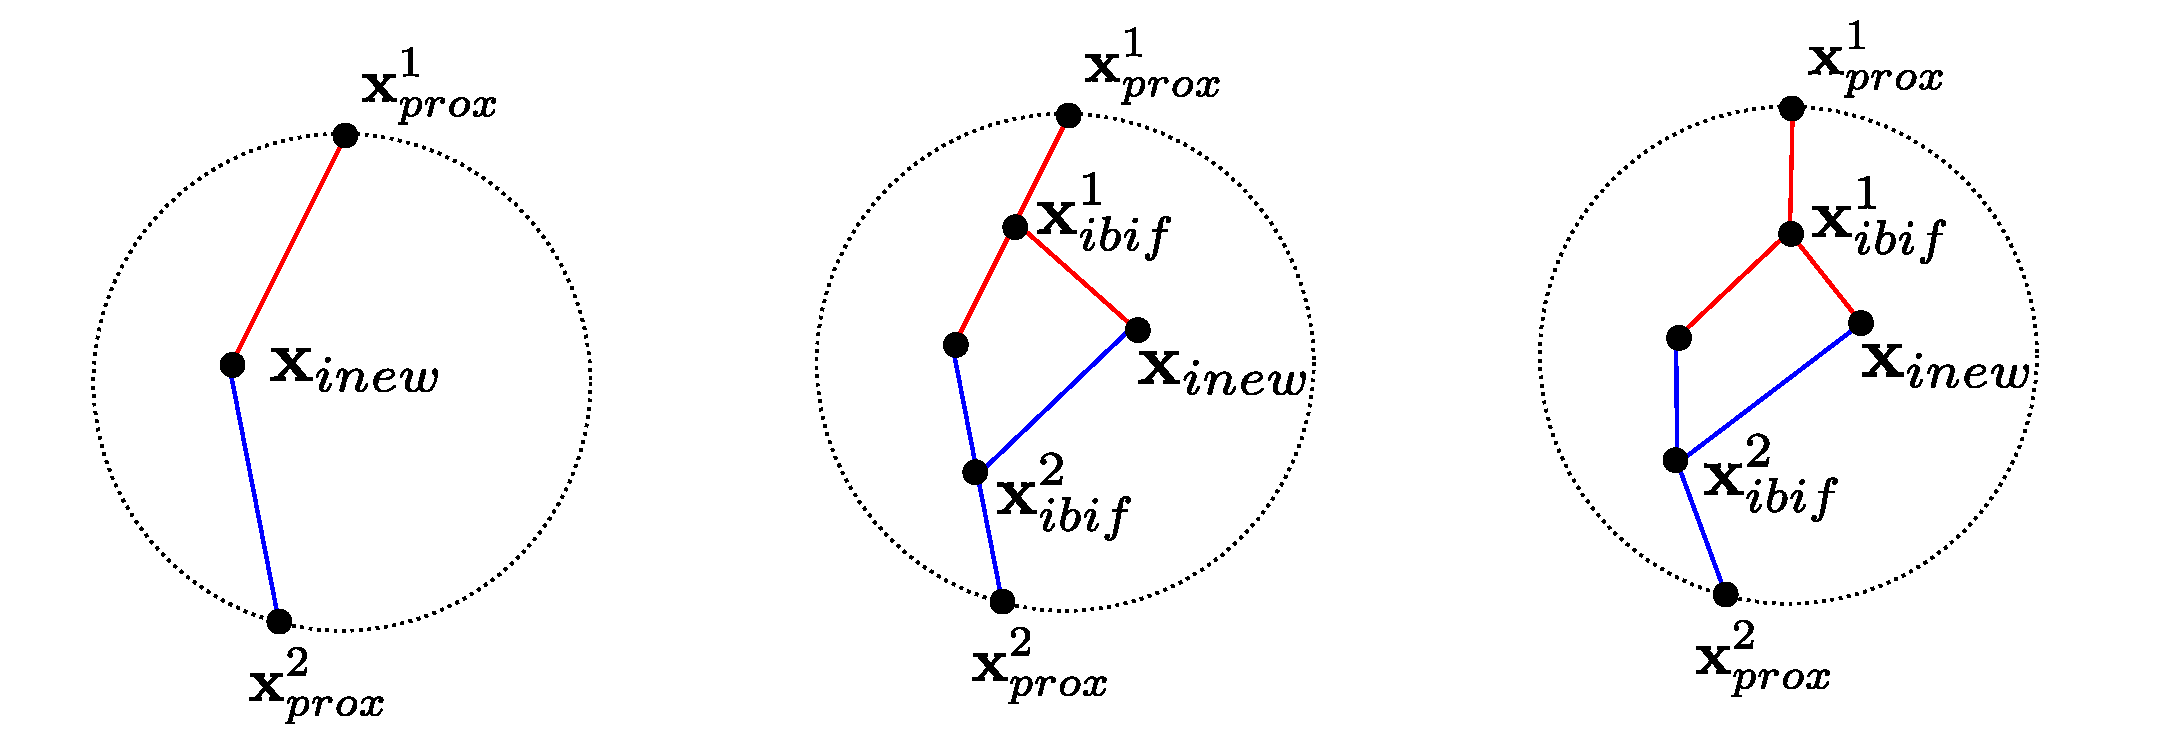
\includegraphics[width = \textwidth]{figuras/modelos-computacionais-de-arvores-circulatorias/passos-algoritmo-arteriovenoso.eps}

  (a) \hspace{0.33\textwidth} (b) \hspace{0.33\textwidth} (c)
  \fonteAutor{2022}
  \label{fig:CCOVenosoArterial}
\end{figure}

\begin{algorithm}
\Dados{$D_{perf}$, $\mathbf{x}_{prox}^t$, $Q_{perf}^t$, $N_{term}$, $\Delta p^t$, $\gamma$, $N_{trees}$.}
  Fixar as posi\c{c}\~oes proximais dos segmentos raízes $\mathbf{x}_{prox}^t$ no domínio de perfusão\; 
  Gerar e validar a posi\c{c}\~ao terminal $\mathbf{x}_{inew}$ dos segmentos raízes\;
  \For{$t \gets 1$ \textbf{até} $N_{trees}$}{
    Conectar $\mathbf{x}_{inew}$ a $\mathbf{x}_{prox}^t$ (\textit{coloca segmento raiz da árvore $t$})\;
  }
  $k_{term} = 1$\;
  \While{($k_{term} < N_{term}$)}{    
    Gerar e validar a posi\c{c}\~ao distal $\mathbf{x}_{inew}$ de um novo segmento terminal\;
    Conectar $\mathbf{x}_{inew}$ a um segmento de cada árvore $t$ criando novas bifurca\c{c}\~oes $\mathbf{x}_{ibif}^t$\;
    Otimizar a posi\c{c}\~ao de $\mathbf{x}_{ibif}^t$\;
    $k_{term} = k_{term} + 1$\;
  }
  \caption{Gera\c{c}ão de sistema vascular arteriovenoso com $N_{trees}$ árvores~\cite{Queiroz2013,Queiroz2018}.}
  \label{algo:CCOVenosoArterial}
\end{algorithm}

O Algoritmo~\ref{algo:CCOVenosoArterial} funciona basicamente como o Algoritmo~\ref{algo:CCOclassico} 
do método CCO, mas vale destacar os seguintes pontos:
\begin{itemize}
 \item para cada árvore $t$ ($t=1,\ldots,N_{trees}$), a posi\c{c}\~ao proximal do segmento raiz ($\mathbf{x}_{prox}^t$), 
 o fluxo no segmento raiz ($Q_{perf}^t$) e a queda de pressão total ($\Delta p^t$) são dados de entrada do algoritmo.
 O valor de $N_{trees}$ pode ser arbitrário, em particular $N_{trees}$ = 2 no caso do sistema vascular 
 renal;
 
 \item tanto na linha 2 como na linha 8 do Algoritmo~\ref{algo:CCOVenosoArterial}, a posi\c{c}\~ao $\mathbf{x}_{inew}$
 gerada (aleatoriamente) só é validada se atender um critério de 
 distância~\cite{Queiroz2013, Schreiner1993b} em rela\c{c}\~ao aos segmentos já existentes 
 de cada árvore $t$ (caso contrário outra posição é gerada);

 \item cada nova posi\c{c}\~ao $\mathbf{x}_{inew}$ será conectada em mais de uma árvore a cada passo; 
  
 \item ao conectar a posi\c{c}\~ao $\mathbf{x}_{inew}$ em segmentos das árvores $t$, criamos novas bifurcações 
 ($\mathbf{x}_{ibif}^t$) que necessitam ser otimizadas em cada árvore de modo a minimizar a sua respectiva 
 função custo~\eqref{eq:volume}.
\end{itemize}

\subsection{Construção de florestas de árvores arteriais}\label{subsec:floresta-vascular}

Em~\cite{Jaquet2019}, é proposto um algoritmo baseado no método CCO, 
resumido conforme o fluxograma ilustrado na Figura~\ref{algo:CCOFlorestaDeArvores}, 
que realiza a construção de uma floresta de árvores vasculares. 
Suponha que serão criadas $N_{trees}$ árvores em um volume de perfusão $D_{perf}$, 
cada uma com um fluxo alvo $q_{targ}^t$, onde $t = 1,\,2,\,\ldots,\,N_{trees}$. 

Inicialmente, os pontos $\mathbf{x}_{inew}^t$ são gerados aleatoriamente. 
Cada ponto $\mathbf{x}_{inew}^t$ é 
considerado válido se estiver dentro do domínio de perfusão e se sua distância ao 
ponto $\mathbf{x}_{root}^t$ (ponto proximal do segmento raiz da árvore $t$) for 
menor ou igual a $l_{max}^t$ dado por:
\begin{equation}
 l_{max}^t = d_{cn}^t \dfrac{q_{targ}^t}{q_{targ}^{cn} + q_{targ}^t},
 \label{eq:criterio.distancia.raiz}
\end{equation}
onde $d_{cn}^t$ é a distância entre o ponto $\mathbf{x}_{root}^t$ 
e o ponto $\mathbf{x}_{root}^i$ (com $i\neq t$) mais próximo 
e $q_{targ}^{cn}$ é o fluxo alvo da árvore $i$. Após esta etapa de geração e validação, 
o ponto $\mathbf{x}_{inew}^t$ será conectado ao ponto $\mathbf{x}_{root}^t$ formando
o segmento raiz da árvore $t$.

Durante o crescimento da floresta é criado uma competição entre as 
árvores para ocupar o domínio de perfusão. Para isso, é analisado o fluxo relativo entre elas.
Supondo que a árvore $b$ tenha o maior fluxo
alvo $q_{targ}^b$, o fluxo relativo da árvore $t\neq b$ no passo $K_{term}$ da
iteração é dado por:
\begin{equation}
 \chi_{K_{term}}^t = \dfrac{q_{K_{term}}^t}{q_{K_{term}}^b}\textrm{.}
 \label{eq:fluxo.relativo.temporario}
\end{equation}

Esse fluxo relativo é comparado com o fluxo alvo relativo:
\begin{equation}
 \chi_{targ}^t = \dfrac{q_{targ}^t}{q_{targ}^b}
 \label{eq:fluxo.relativo.total}
\end{equation}

Define-se que a árvore $t$ está ativa se $\chi_{targ}^t > \chi_{K_{term}}^t$ e como
inativa caso contrário. Em relação a árvore $b$, marca-se como ativa se
$q_{targ}^b > q_{K_{term}}^b$ e como inativa caso contrário. A cada passo do processo de
crescimento da floresta, um novo segmento terminal é adicionado a uma das árvores ativas 
de modo que o volume total da floresta (isto é, a soma dos volumes de cada árvore calculado 
conforme~\eqref{eq:volume}) seja mínimo.

\begin{figure}
  \centering
  \caption{Fluxograma do algoritmo de gera\c{c}ão de floresta de árvores vasculares conforme~\cite{Jaquet2019}.}
  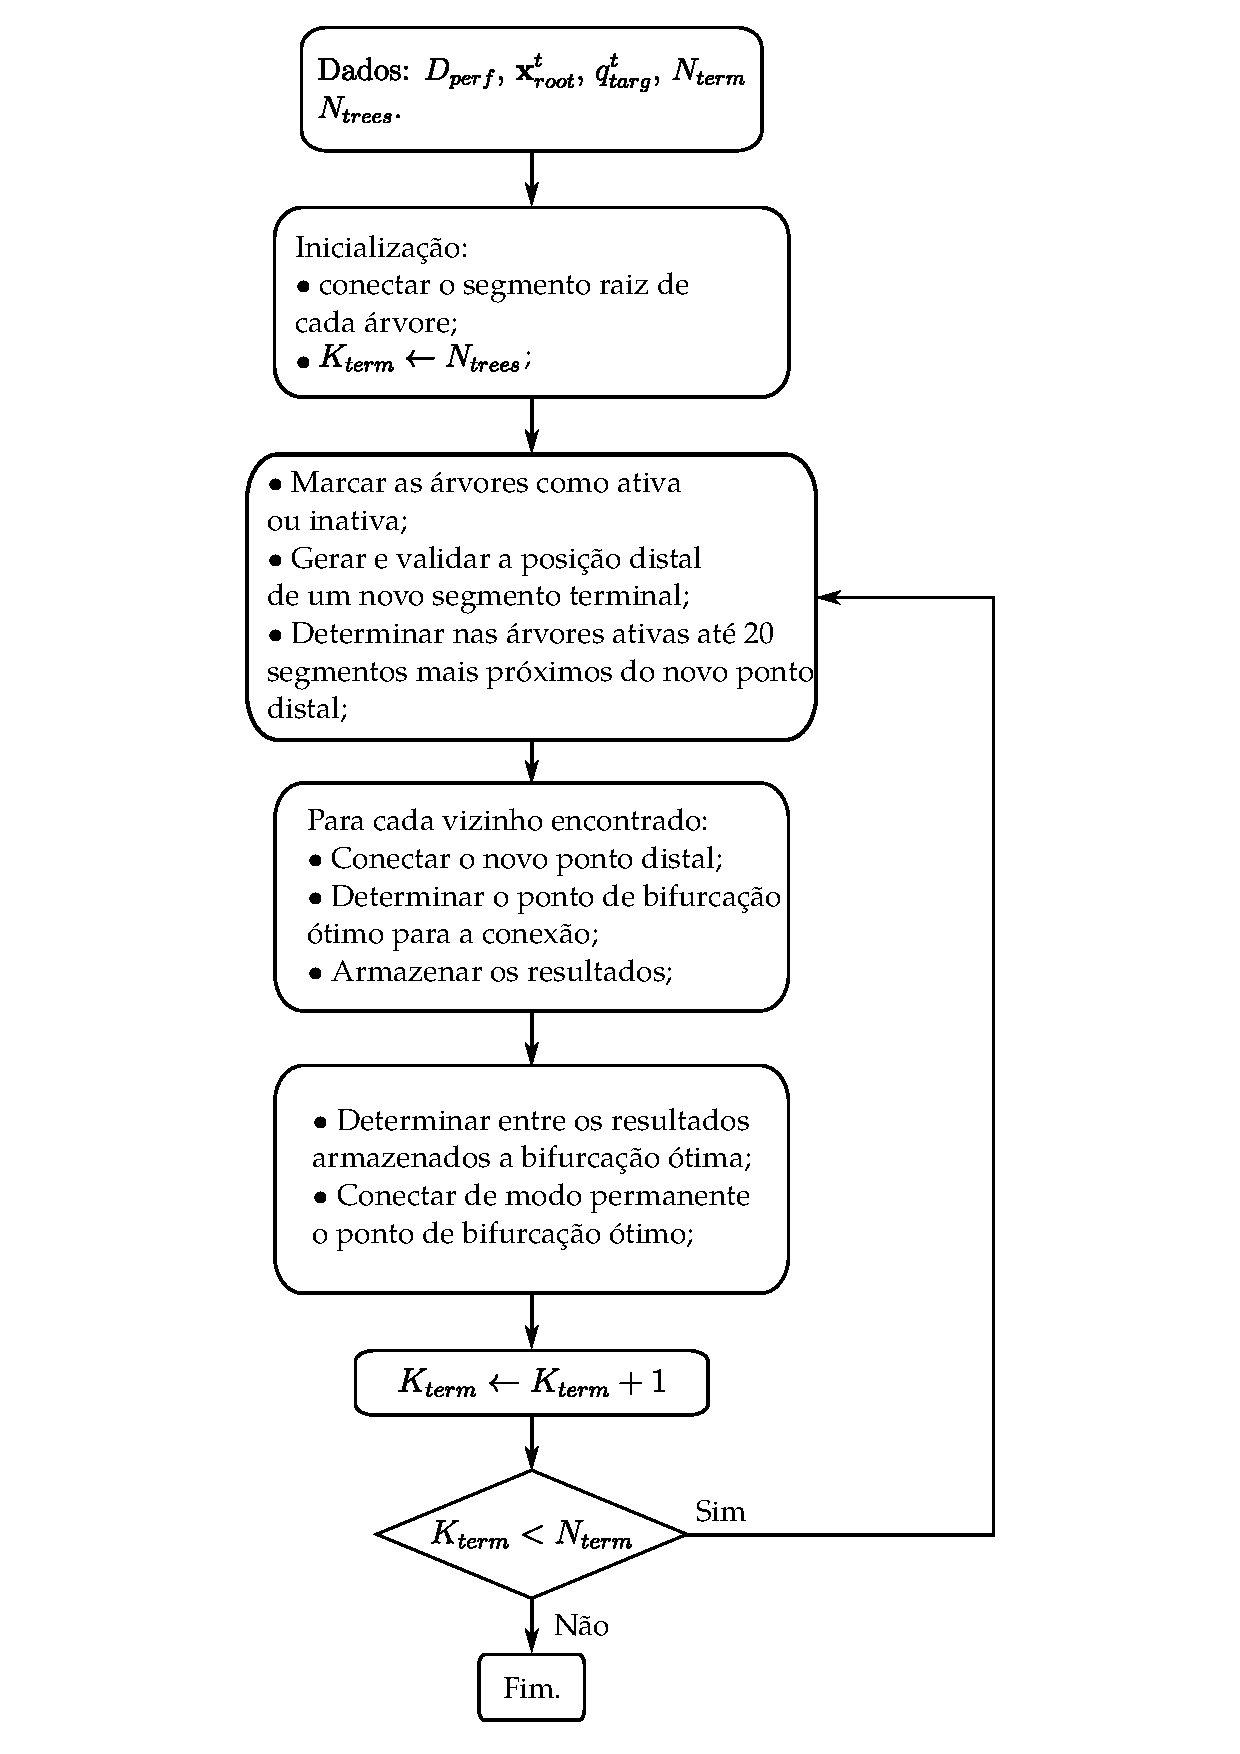
\includegraphics[scale=0.75]{figuras/modelos-computacionais-de-arvores-circulatorias/fluxograma-algoritmo-jaquet.pdf}
  \fonteAutor{2022}
  \label{algo:CCOFlorestaDeArvores}
\end{figure}

Para o ponto $\mathbf{x}_{inew}$ ser válido o segmento mais próximo dele deve estar em uma 
árvore ativa. Considerando as árvores ativas para as quais $\mathbf{x}_{inew}$ for válido, 
são encontrados os $N \leq 20$ segmentos mais próximos deste ponto (isto é, aqui considera-se 
$N_{con} = 20$ conforme~\cite{Karch1999}). Para cada segmento encontrado, 
uma conexão temporária é determinada e otimizada 
seguindo ideias semelhantes ao método CCO explicadas na Seção~\ref{sec:cco}
(a otimização geométrica da conexão é feita como em~\cite{Kamiya1972}).

Para determinar os subdomínios ocupados em cada simulação, foi 
construído um Diagrama de Voronoi~\cite{Aurenhammer2004}. Dados os pontos distais dos terminais das 
árvores, $P_1$, $P_2$, \ldots, $P_n$ (com $n = N_{term}$),
o domínio de perfusão $D_{perf}$ é dividido em 
$n$ subregiões $D_1$, $D_2$, \ldots, $D_n$ tais que:
\begin{equation}
 D_i = \{P\in D_{perf} \,|\, \dist(P,P_i) < \dist(P, P_j),\, \forall j\neq i\}\textrm{.}
 \label{def:diagrama-voronoi}
\end{equation}

O território ocupado por uma árvore $t$ será composto pela união das subregiões 
$D_i$ tais que $P_i$ seja um ponto pertencente à árvore $t$. Em~\cite{Jaquet2019}, 
é exibido que o território ocupado por uma árvore $t$ segue um percentual (em relação 
ao território total do domínio de perfusão $D_{perf}$) que é compatível com o percentual 
dos fluxos alvo (em relação ao fluxo total na floresta).

Apesar do algoritmo proposto em~\cite{Jaquet2019} implementar uma estratégia de competição 
pelo fluxo de sangue entre as árvores na floresta (através da comparação 
entre $\chi_{K_{term}}^t$ e $\chi_{targ}^t$), não há no algoritmo um parâmetro 
que permita controlar a invasão de uma árvore no território da outra. 
Na Seção~\ref{sec:floresta-com-invasao} é discutida uma estratégia para
implementar esse controle.

\chapter{ALGORITMOS PROPOSTOS PARA CONSTRUÇÃO DE FLORESTA DE ÁRVORES ARTERIAIS} \label{sec:algoritmos-propostos}

Neste capítulo, apresenta-se os algoritmos propostos nesta tese para gerar florestas de árvores 
arteriais concorrentes e que não se comunicam.

Diferentemente dos algoritmos apresentados na Seção~\ref{sec:construcao-de-multiplas-arvores}, 
os algoritmos desenvolvidos podem incorporar no processo de geração das florestas 
um controle de invasão das árvores, bem como a geração em estágios de crescimento através 
de uma estratégia baseada no diagrama de Voronoi~\cite{Aurenhammer2004}.

\section{CONSTRUÇÃO DE FLORESTAS DE ÁRVORES ARTERIAIS COM COEFICIENTE DE INVASÃO} \label{sec:floresta-com-invasao}

Para permitir um controle melhor da invasão de uma árvore no território da outra, é proposto 
neste trabalho o Algoritmo~\ref{algo:FlorestaDeArvoresComInvasao} 
(baseado em~\cite{Jaquet2019}). Para obter esse controle, 
em relação à árvore $t$, admite-se o ponto $\mathbf{x}_{inew}$ 
como posição distal de um novo segmento terminal se atender as condições:
\begin{enumerate}[label=(\roman*)]
 \item estiver dentro do domínio de perfusão;
 \item sua distância 
até $\mathbf{x}_{root}^t$ for menor ou igual a $l_{max}^t$ 
(conforme definido em~\eqref{eq:criterio.distancia.raiz}). Essa condição 
só é considerada enquanto o fluxo atual da árvore $t$ for menor ou igual a $\alpha q^t_{targ}$, 
onde $\alpha\in[0,\,1]$ é um coeficiente constante de invasão. Quanto mais próximo $\alpha$ estiver de $1$, menos 
uma árvore invade o território vascular da outra;
 \item sua distância a todos os segmentos da árvore $t$ for maior do que 
 \begin{equation}
   d_{min} = \sqrt[n]{\dfrac{|D_{perf}|}{K_{term}}}
   \label{eq:distancia-minima}
 \end{equation}
 onde $n = 2$ (no caso bidimensional) ou 
 $n = 3$ (no caso tridimensional), $|D_{perf}|$ é a área de $D_{perf}$ (ou o volume, conforme valor de $n$)
 e $K_{term}$ é a soma do número de segmentos terminais de todas as árvores no passo atual. Nota-se que 
 geometricamente $d_{min}$ vai representar o lado do quadrado (ou aresta do cubo) de uma unidade 
 de área (ou unidade de volume) delimitada por $D_{perf}$.
\end{enumerate}

A Figura~\ref{fig:passos-metodo-proposto} ilustra o funcionamento básico do Algoritmo~\ref{algo:FlorestaDeArvoresComInvasao}.

\begin{algorithm}
  \Dados{
    $D_{perf}$, $\mathbf{x}_{root}^t$, $q_{targ}^t$, $N_{term}$,
    $N_{con}$, $N_{trees}$, $\eta$, $\alpha$, $\beta$.
  }
  Gerar e validar uma posi\c{c}\~ao distal $\mathbf{x}_{inew}^t$ do 
  segmento raiz da árvore $t=1,\,2,\,\ldots,\,N_{tree}$, respeitando a distância 
  $l_{max}^t$\;
  Conectar $\mathbf{x}_{inew}^t$ a $\mathbf{x}_{root}^t$ (\textit{plantar o segmento raiz da árvore }$t$)\;
  \For{($K_{term}\gets 1$ \KwTo $N_{term}$)}{
    Marcar as árvores como ativa ou inativa, baseado no seu fluxo atual\;
    Gerar a posi\c{c}\~ao distal $\mathbf{x}_{inew}$ de um novo segmento terminal e 
    verificar as condições (i), (ii) e (iii)\;
    Determinar $N \leq N_{con}$ segmentos que estão mais próximos de $\mathbf{x}_{inew}$ nas 
    árvores ativas\;
    \For{($j\gets 0$ \KwTo N)}{
      Conectar $\mathbf{x}_{inew}$ temporariamente no segmento $j$, 
      criando a bifurca\c{c}\~ao $\mathbf{x}_{ibif}$\;
      Otimizar e validar a posi\c{c}\~ao de $\mathbf{x}_{ibif}$\;    
      Armazenar resultados de $\mathbf{x}_{ibif}$ na TAC\;
      Descartar conexão temporária $\mathbf{x}_{ibif}$\;
    }
    Obter TAC$_r$ a partir de TAC removendo as conexões inválidas\;
    Determinar em TAC$_r$ a bifurcação ótima $\mathbf{x}_{iopt}$\;
    Conectar $\mathbf{x}_{inew}$ a $\mathbf{x}_{iopt}$ de modo permanente\;
  }
\caption{Gera\c{c}ão de floresta de árvores arteriais com coeficiente de invasão.}
\label{algo:FlorestaDeArvoresComInvasao}
\end{algorithm}

\begin{figure}[!htb]
  \centering
  \captiondelim{: }
  \caption{Ilustração dos passos básicos do Algoritmo~\ref{algo:FlorestaDeArvoresComInvasao} no crescimento 
    de uma floresta com $N_{trees} = 2$. 
    (a) O ponto $\mathbf{x}_{inew}$ é escolhido aleatoriamente dentro do domínio de perfusão. 
    Testa-se a conexão desse ponto com os $N \leq N_{con}$ segmentos mais próximos 
    nas árvores ativas. Será feita permanente a conexão que fornecer o menor volume total. 
    (b) Exemplo do teste de conexão do ponto $\mathbf{x}_{inew}$ com
    um segmento próximo na árvore 1.
    (c) Exemplo do teste de conexão do ponto $\mathbf{x}_{inew}$ com
    um segmento próximo na árvore 2.
  }
  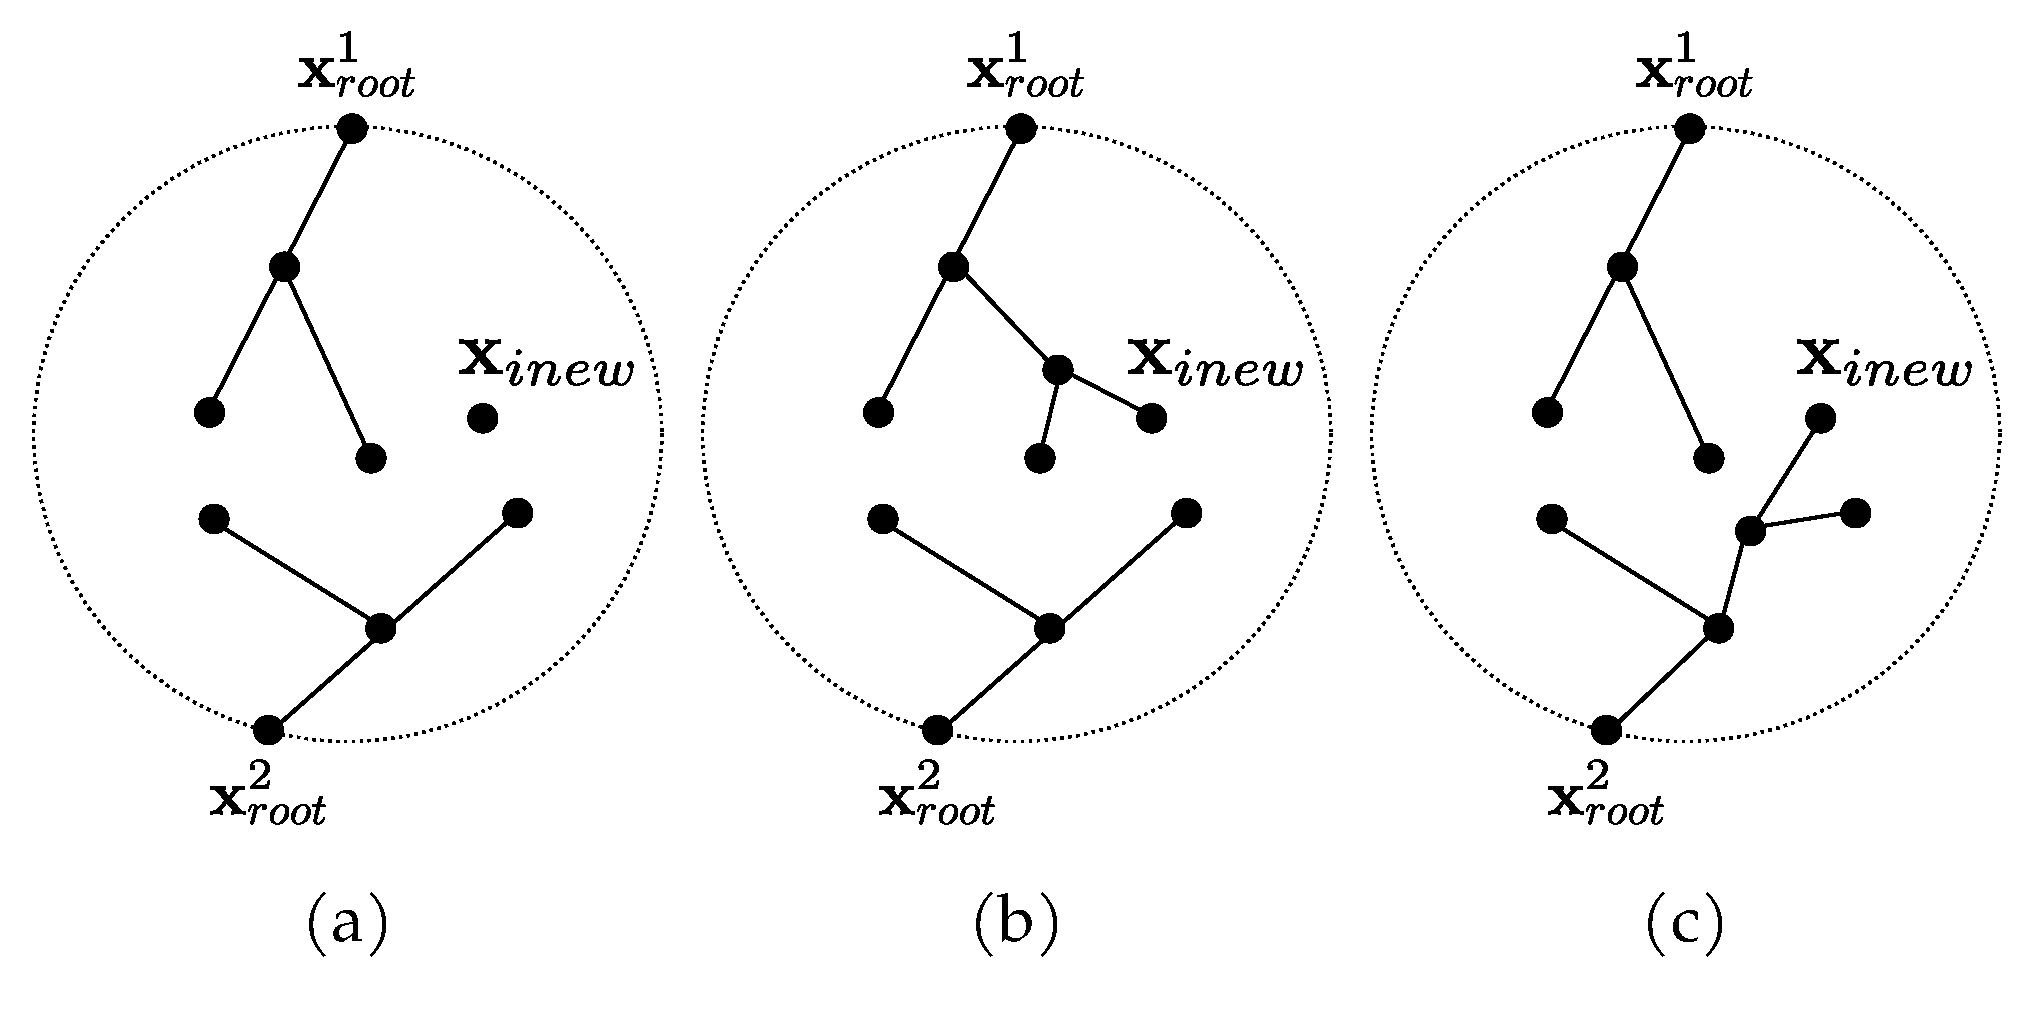
\includegraphics[scale=0.4]{figuras/modelos-computacionais-de-arvores-circulatorias/passos-algoritmo-cco-narvores.eps}
  \fonteAutor{2022}
  \label{fig:passos-metodo-proposto}
\end{figure}

Para otimizar a posição $\mathbf{x}_{ibif}$ na iteração mais
interna do Algoritmo~\ref{algo:FlorestaDeArvoresComInvasao}, utilizou-se a 
estratégia de mapeamento~\eqref{eq:mapeamento-bifucacao} como mencionada na 
Seção~\ref{subsec:arvores-arterial-venosa}.

Conforme explicado na Seção~\ref{subsec:floresta-vascular}, o ponto $\mathbf{x}_{inew}$ será 
válido somente se o segmento mais próximo dele estiver em uma 
árvore ativa. Caso necessário, deve-se gerar aleatoriamente outras posições 
até que $\mathbf{x}_{inew}$ seja válido. O critério de distância presente na 
condição (iii) pode ser muito restritivo e o processo aleatório de geração pode 
ser repetido muitas vezes. Para relaxar esse critério, 
se a geração de $\mathbf{x}_{inew}$ for repetida $N_{toss}$ vezes sem conseguir 
obter uma posição que atenda (iii), então $d_{min}$ será atualizado como 
$\beta d_{min}$, onde $\beta\in (0,\,1)$ é um fator de redução. Além disso, 
$d_{min}$ também será atualizado se por $N_{toss}$ vezes a posição atender 
(iii), mas não for possível obter uma bifurcação ótima $\mathbf{x}_{iopt}$.

\section{CONSTRUÇÃO DE FLORESTAS DE ÁRVORES ARTERIAIS EM ESTÁGIOS} \label{sec:coat}

O algoritmo proposto na Seção~\ref{sec:floresta-com-invasao} utiliza a estratégia de 
modificar o método CCO de modo a construir mais de uma árvore simultaneamente 
sem subdividir o domínio de perfusão. Por outro lado, para explorar a estratégia de 
subdividir o domínio de perfusão e construir cada árvore da floresta no seu respectivo
subdomínio, nesta seção é proposto um algoritmo chamado \textit{Competing Optimized Arterial Trees} 
(COAT) que é baseado no método CCO.

Suponha que deseja-se construir $N_{trees}$ árvores binárias em um domínio de perfusão $D_{perf}$, 
cada uma com um fluxo alvo $q_{targ}^t$, onde $t = 1,\,2,\,\ldots,\,N_{trees}$.
Durante o crescimento da floresta é criado uma competição entre as 
árvores para ocupar o domínio $D_{perf}$. Para isso, é analisado o fluxo relativo entre elas
(conforme~\eqref{eq:fluxo.relativo.temporario} e~\eqref{eq:fluxo.relativo.total}).

O Algoritmo~\ref{algo:COAT} representa o COAT. Ele 
gera uma floresta de árvores circulatórias em dois estágios. 
No primeiro estágio, o domínio de perfusão será ocupado por 
uma floresta inicial. 
Essa floresta inicial pode ser construída automaticamente durante esse estágio 
conforme Seção~\ref{subsec:construcao-floresta-inicial}. Além disso, esta floresta inicial 
pode ser obtida através da reconstrução de imagens médicas de tomografia 
computadorizada, por exemplo. Inicialmente, essa floresta pode ainda ser gerada 
empregando o algoritmo proposto de controle de invasão descrito na Seção~\ref{sec:floresta-com-invasao}.

Em seguida, a floresta 
inicial é usada para dividir o domínio de perfusão em subdomínios 
disjuntos, cada um associado a uma das árvores.
No segundo estágio, as árvores na floresta continuarão 
o seu crescimento dentro do seu respectivo subdomínio.

\subsection{Construção automática da floresta inicial no primeiro estágio}\label{subsec:construcao-floresta-inicial}

Uma maneira de construir a floresta inicial durante o primeiro estágio pode 
ser conforme explicado a seguir. Inicialmente, são gerados aleatoriamente 
pontos $\mathbf{x}_{inew}^t$ que serão candidatos a ponto distal 
dos segmentos raízes das árvores. Cada ponto $\mathbf{x}_{inew}^t$ é 
considerado válido se estiver dentro do domínio de perfusão e se sua distância ao 
ponto $\mathbf{x}_{root}^t$ (ponto proximal do segmento raiz da árvore $t$) for 
menor ou igual a $l_{max}^t$ (conforme definido em~\eqref{eq:criterio.distancia.raiz}).
Após esta etapa de geração e validação, 
o ponto $\mathbf{x}_{inew}^t$ será conectado ao ponto $\mathbf{x}_{root}^t$ formando
o segmento raiz da árvore $t$.

Em seguida, serão adicionados mais terminais em cada árvore $t$ na floresta.
Admite-se o ponto $\mathbf{x}_{inew}$ 
como posição distal de um novo segmento terminal se ele atender as condições:
\begin{enumerate}[label=(\roman*)]
 \item estiver dentro do domínio de perfusão;
 \item sua distância 
até $\mathbf{x}_{root}^t$ for menor ou igual a $l_{max}^t$ 
(conforme definido em~\eqref{eq:criterio.distancia.raiz});
 \item sua distância a todos os segmentos da árvore $t$ for maior do que 
 $d_{min}^t$ (conforme definido em ~\eqref{eq:distancia-minima}).
\end{enumerate}

Quando o fluxo da árvore $t$ for igual a $\alpha q_{targ}^t$, onde 
$\alpha\in(0,1)$ é chamado de coeficiente de estágio,
ela será marcada como inativa e deixará de receber novos segmentos terminais.
A construção da floresta inicial estará finalizada quando todas as suas árvores
estiverem marcadas como inativas.

\subsection{Divisão do domínio de perfusão}\label{subsec:divisao-do-dominio-de-perfusao}

Após o primeiro estágio, o domínio de perfusão $D_{perf}$ é dividido em subdomínios 
disjuntos $D_1$, $D_2$, \ldots, $D_{N_{trees}}$. Para efetuar esse processo uma 
estratégia baseada na ideia do diagrama de Voronoi~\cite{Aurenhammer2004} é utilizada,
considerando como pontos de referência os pontos distais dos segmentos da árvore $t$.
Suponha que $P_{cn}^t$ seja o ponto distal na árvore $t$ que está mais próximo de um ponto $P$ do
domínio de perfusão. O subdomínio $D_t$ será composto pelos pontos 
$P$ tais que:
\begin{equation}
  \begin{cases}
	\mathrm{dist}(P,\,P_{cn}^t) < \mathrm{dist}(P, P_{cn}^k),\, \forall k\neq t;\,\textrm{ se }\mathrm{dist}(P,\,P_{cn}^t) < \lambda\max \mathrm{dist}(P, P_{cn}^k)\\
	q_{targ}^t < q_{targ}^k,\, \forall k\neq t;\,\textrm{ caso contr\'ario}\\
  \end{cases},
  \label{def:diagrama-voronoi-coat}
\end{equation}
onde $\lambda\in(0, 1]$ é um peso. Quanto mais próximo de 0 é esse peso, 
mais os fluxos alvo são priorizados durante a subdivisão. Por outro lado, quanto
mais próximo 1, mais será priorizado a distância entre os pontos $P$ e $P_{cn}^t$.

A Figura~\ref{fig:exemplo-construcao-diagrama-voronoi} ilustra um exemplo para determinar 
se um ponto $P$ do domínio de perfusão $D_{perf}$ pertence à região $D_1$ ou $D_2$,
considerando que $\lambda = \dfrac{1}{2}$ e na floresta há duas árvores com $q_{targ}^1 < q_{targ}^2$.
A ideia básica nessa estratégia de divisão é que sempre que um ponto 
$P$ está suficientemente próximo de uma árvore $t$, então ele estará no subdomínio
$D_t$. Entretanto, quando um ponto $P$ está aproximadamente equidistante
de todas as árvores, então o ponto $P$ estará no subdomínio $D_t$ que tem
o menor fluxo alvo ($q_{targ}^t$). Isso ajuda a aumentar o território ocupado pela
árvore com menor fluxo. Caso contrário, esse território ficaria
menor do que o desejado.

\clearpage

\begin{figure}[!htb]
  \centering \captiondelim{: }
  \caption{Determinar se $P$ pertence à $D_1$ ou $D_2$, considerando duas 
  árvores com $q_{targ}^1 < q_{targ}^2$ e $\lambda = \dfrac{1}{2}$.
  (a) $P$ vai pertencer à $D_2$, pois 
  $\mathrm{dist}(P,\,P_{cn}^2) < \dfrac{1}{2}\mathrm{dist}(P,\,P_{cn}^1)$.
  (b) $P$ vai pertencer à $D_1$, pois 
  $\mathrm{dist}(P,\,P_{cn}^2) \geq \dfrac{1}{2}\mathrm{dist}(P,\,P_{cn}^1)$
  e $q_{targ}^1 < q_{targ}^2$.
  }
  
  \subfloat[][]{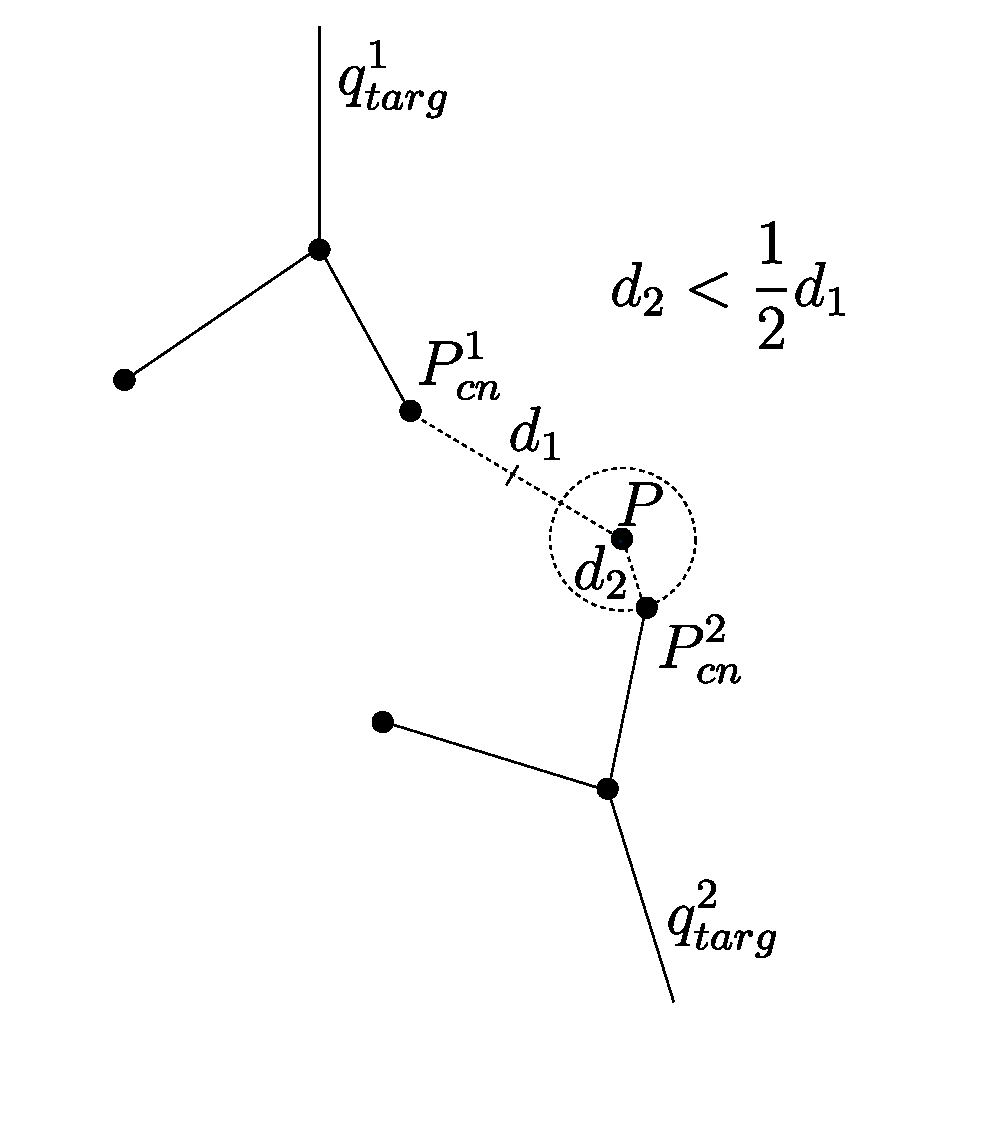
\includegraphics[scale=0.4]{figuras/competing-optimized-arterial-trees/exemplo-construcao-diagrama-voronoi-a.pdf}}
  \hspace{12pt}
  \subfloat[][]{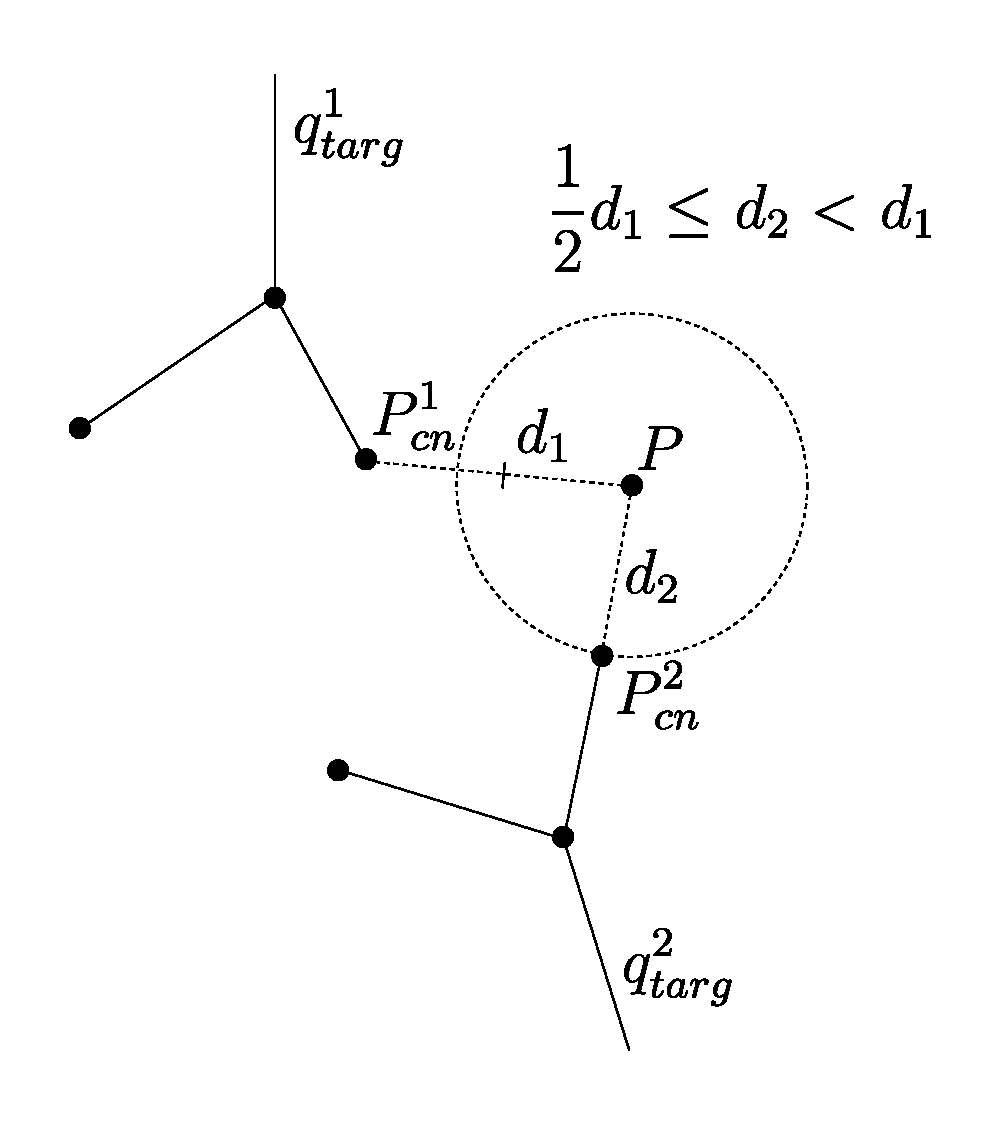
\includegraphics[scale=0.4]{figuras/competing-optimized-arterial-trees/exemplo-construcao-diagrama-voronoi-b.pdf}}

  \fonteAutor{2022}\label{fig:exemplo-construcao-diagrama-voronoi}
\end{figure}

\subsection{Construção da floresta no segundo estágio}\label{subsec:construcao-da-floresta-segundo-estagio}

No segundo estágio, cada árvore $t$ continua o seu crescimento. Admite-se o 
ponto $\mathbf{x}_{inew}$ como posição distal de um novo segmento terminal
se ele atender as condições:
\begin{enumerate}[label=(\Roman*)]
 \item estiver dentro do subdomínio $D_t$;
 \item sua distância a todos os segmentos da árvore $t$ for maior do que 
 $d_{min}^t$ (conforme definido em ~\eqref{eq:distancia-minima});
\end{enumerate}

\begin{algorithm}
\Dados{
  $D_{perf}$, $\mathbf{x}_{root}^t$, $q_{targ}^t$, 
  $N_{term}$, $N_{trees}$, $\alpha$, $N_{con}$, 
  $\beta$, $\eta$, $\lambda$.
}

  \textit{\underline{Primeiro estágio:}} abrir (ou construir) a floresta inicial\;
  Dividir $D_{perf}$ em subdomínios disjuntos $D_1$, $D_2$, \ldots, $D_{N_{trees}}$\;
  $K_{term}\leftarrow$ número atual de segmentos terminais na floresta\;
  \textit{\underline{Segundo estágio:}}
  \While{($K_{term} < N_{term}$)}{
    Gerar a posi\c{c}\~ao distal $\mathbf{x}_{inew}$ e verificar a qual subdomínio $D_i$
    ela pertence\;
    Verificar as condições (I) e (II) para $\mathbf{x}_{inew}$\;
    Determinar $N \leq N_{con}$ segmentos que estão mais próximos de $\mathbf{x}_{inew}$ na 
    árvore $i$\;
    \For{($j\gets 0$ \KwTo N)}{
      Conectar $\mathbf{x}_{inew}$ temporariamente no segmento $j$, 
      criando a bifurca\c{c}\~ao $\mathbf{x}_{ibif}$\;
      Otimizar e validar a posi\c{c}\~ao de $\mathbf{x}_{ibif}$\;    
      Armazenar resultados de $\mathbf{x}_{ibif}$ na TAC\;
      Descartar conexão temporária $\mathbf{x}_{ibif}$\;
    }
    Obter a TAC$_r$ a partir de TAC removendo as conexões inválidas\;
    Determinar em TAC$_r$ a bifurcação ótima $\mathbf{x}_{iopt}$\;
    Conectar $\mathbf{x}_{inew}$ a $\mathbf{x}_{iopt}$ de modo permanente\;
	$K_{term}\gets K_{term} + 1$\;
  }
\caption{Gera\c{c}ão de floresta de árvores vasculares pelo COAT.}
\label{algo:COAT}
\end{algorithm}

O critério de distância presente nas 
condições (iii) e (II) pode ser muito restritivo e o processo aleatório de geração de 
$\mathbf{x}_{inew}$ pode ser repetido muitas vezes. Para relaxar esse critério, 
se a geração de $\mathbf{x}_{inew}$ for repetida $N_{toss}$ vezes sem conseguir 
obter uma posição que atenda (iii) (ou (II)), então $d_{min}$ será atualizado como 
$\beta d_{min}$, onde $\beta\in (0,\,1)$ é um fator de redução. Além disso, 
$d_{min}$ também será atualizado se por $N_{toss}$ vezes a posição atender 
(iii) (ou (II)), mas não for possível obter uma bifurcação ótima $\mathbf{x}_{iopt}$.


\chapter{RESULTADOS ALOMÉTRICOS E MORFOMÉTRICOS}\label{sec:resultados-alometricos-morfometricos}

Nesta seção apresenta-se os resultados alométricos e morfométricos obtidos com os modelos gerados pelos Algoritmos~\ref{algo:CCOVenosoArterial},~\ref{algo:FlorestaDeArvoresComInvasao} e~\ref{algo:COAT}.
O Algoritmo~\ref{algo:CCOVenosoArterial} foi implementado na linguagem de programação C por 
Queiroz~\cite{Queiroz2013}. Os demais algoritmos propostos foram implementados na linguagem 
de programação C++. 
A visualização dos modelos gerados nas simulações foi realizada usando o programa de visualização científica 
ParaView~\cite{Ayachit2015} (versão 5.8.1).
O computador usado para executar as simulações dos algoritmos tem processador Intel Pentium G4560 (dual core 
de 3,5 GHz), memória RAM DDR4 de 8 GB e sistema operacional Ubuntu 22.04.

\section{ÁRVORES ARTERIAIS E VENOSAS ACOPLADAS}\label{sec:resultados-arvores-acopladas}

Como estudo de caso, um exemplo da aplicação do Algoritmo~\ref{algo:CCOVenosoArterial} é apresentado  
para a criação de um modelo do sistema vascular arteriovenoso renal que é formado por duas árvores. 
Na Tabela~\ref{tab:parametros-modelo-rim} tem-se os parâmetros utilizados nas simulações, 
que estão de acordo com \cite{Kretowski2004} em relação às condi\c{c}\~oes de contorno de pressão.
A posição proximal do segmento raiz de cada árvore do sistema renal foi aqui 
determinada a partir da rede vascular do atlas digital Anatomium$^{\text{TM}}$~\cite{Langenkamp2015} 
e da localização dos ramos principais de cada árvore mostrada em \cite{Kretowski2004}.
A superfície do domínio de perfusão representando o rim também foi determinada a partir do mesmo atlas.

\begin{table}[!htb]
\centering
\captiondelim{: }
\caption{Parâmetros utilizados para a gera\c{c}\~ao do sistema vascular renal.}
 \begin{tabular}{|c|cc|}
\hline
Parâmetro             &Árvore arterial & Árvore venosa\\
\hline
   $p^t_{perf}$ (mmHg) & 95 & 10 \\
   $p^t_{term}$ (mmHg) & 15 & 5 \\
\hline
   $Q^t_{perf}$ (mL/min) & \multicolumn{2}{|c|}{617,5}\\
$Q^t_{term}$ (mL/min) & \multicolumn{2}{|c|}{0,19297}\\
 $N_{term}$ & \multicolumn{2}{|c|}{3200}\\
$D_{perf}$  (cm$^3$) & \multicolumn{2}{|c|}{57,01} \\
$\gamma$  & \multicolumn{2}{|c|}{2,2} \\
\hline
\end{tabular}
\fonte{Queiroz (2018).}
\label{tab:parametros-modelo-rim}
\end{table}

Na Figura~\ref{fig:resRim3DAcopla} são exibidas as árvores vasculares geradas para 
um domínio representando o rim utilizando o  
Algoritmo~\ref{algo:CCOVenosoArterial}. Destaca-se nesta figura que as árvores 
não estão distribuídas espacialmente de modo uniforme no domínio representando 
o rim humano, isto ocorre por não ter sido utilizado uma distribuição uniforme de 
pontos terminais dentro deste domínio. Isto é compatível com a anatomia deste 
órgão, pois sua vascularização tende a se localizar na sua parênquima, 
ou seja, na região funcional do volume ocupado pela superfície 
envolvente do órgão, que no caso do rim se encontra sobre a região periférica do seu volume.

\begin{figure}[!htb]
  \centering
  \captiondelim{: }
  \caption{Sistema vascular renal gerado.}
  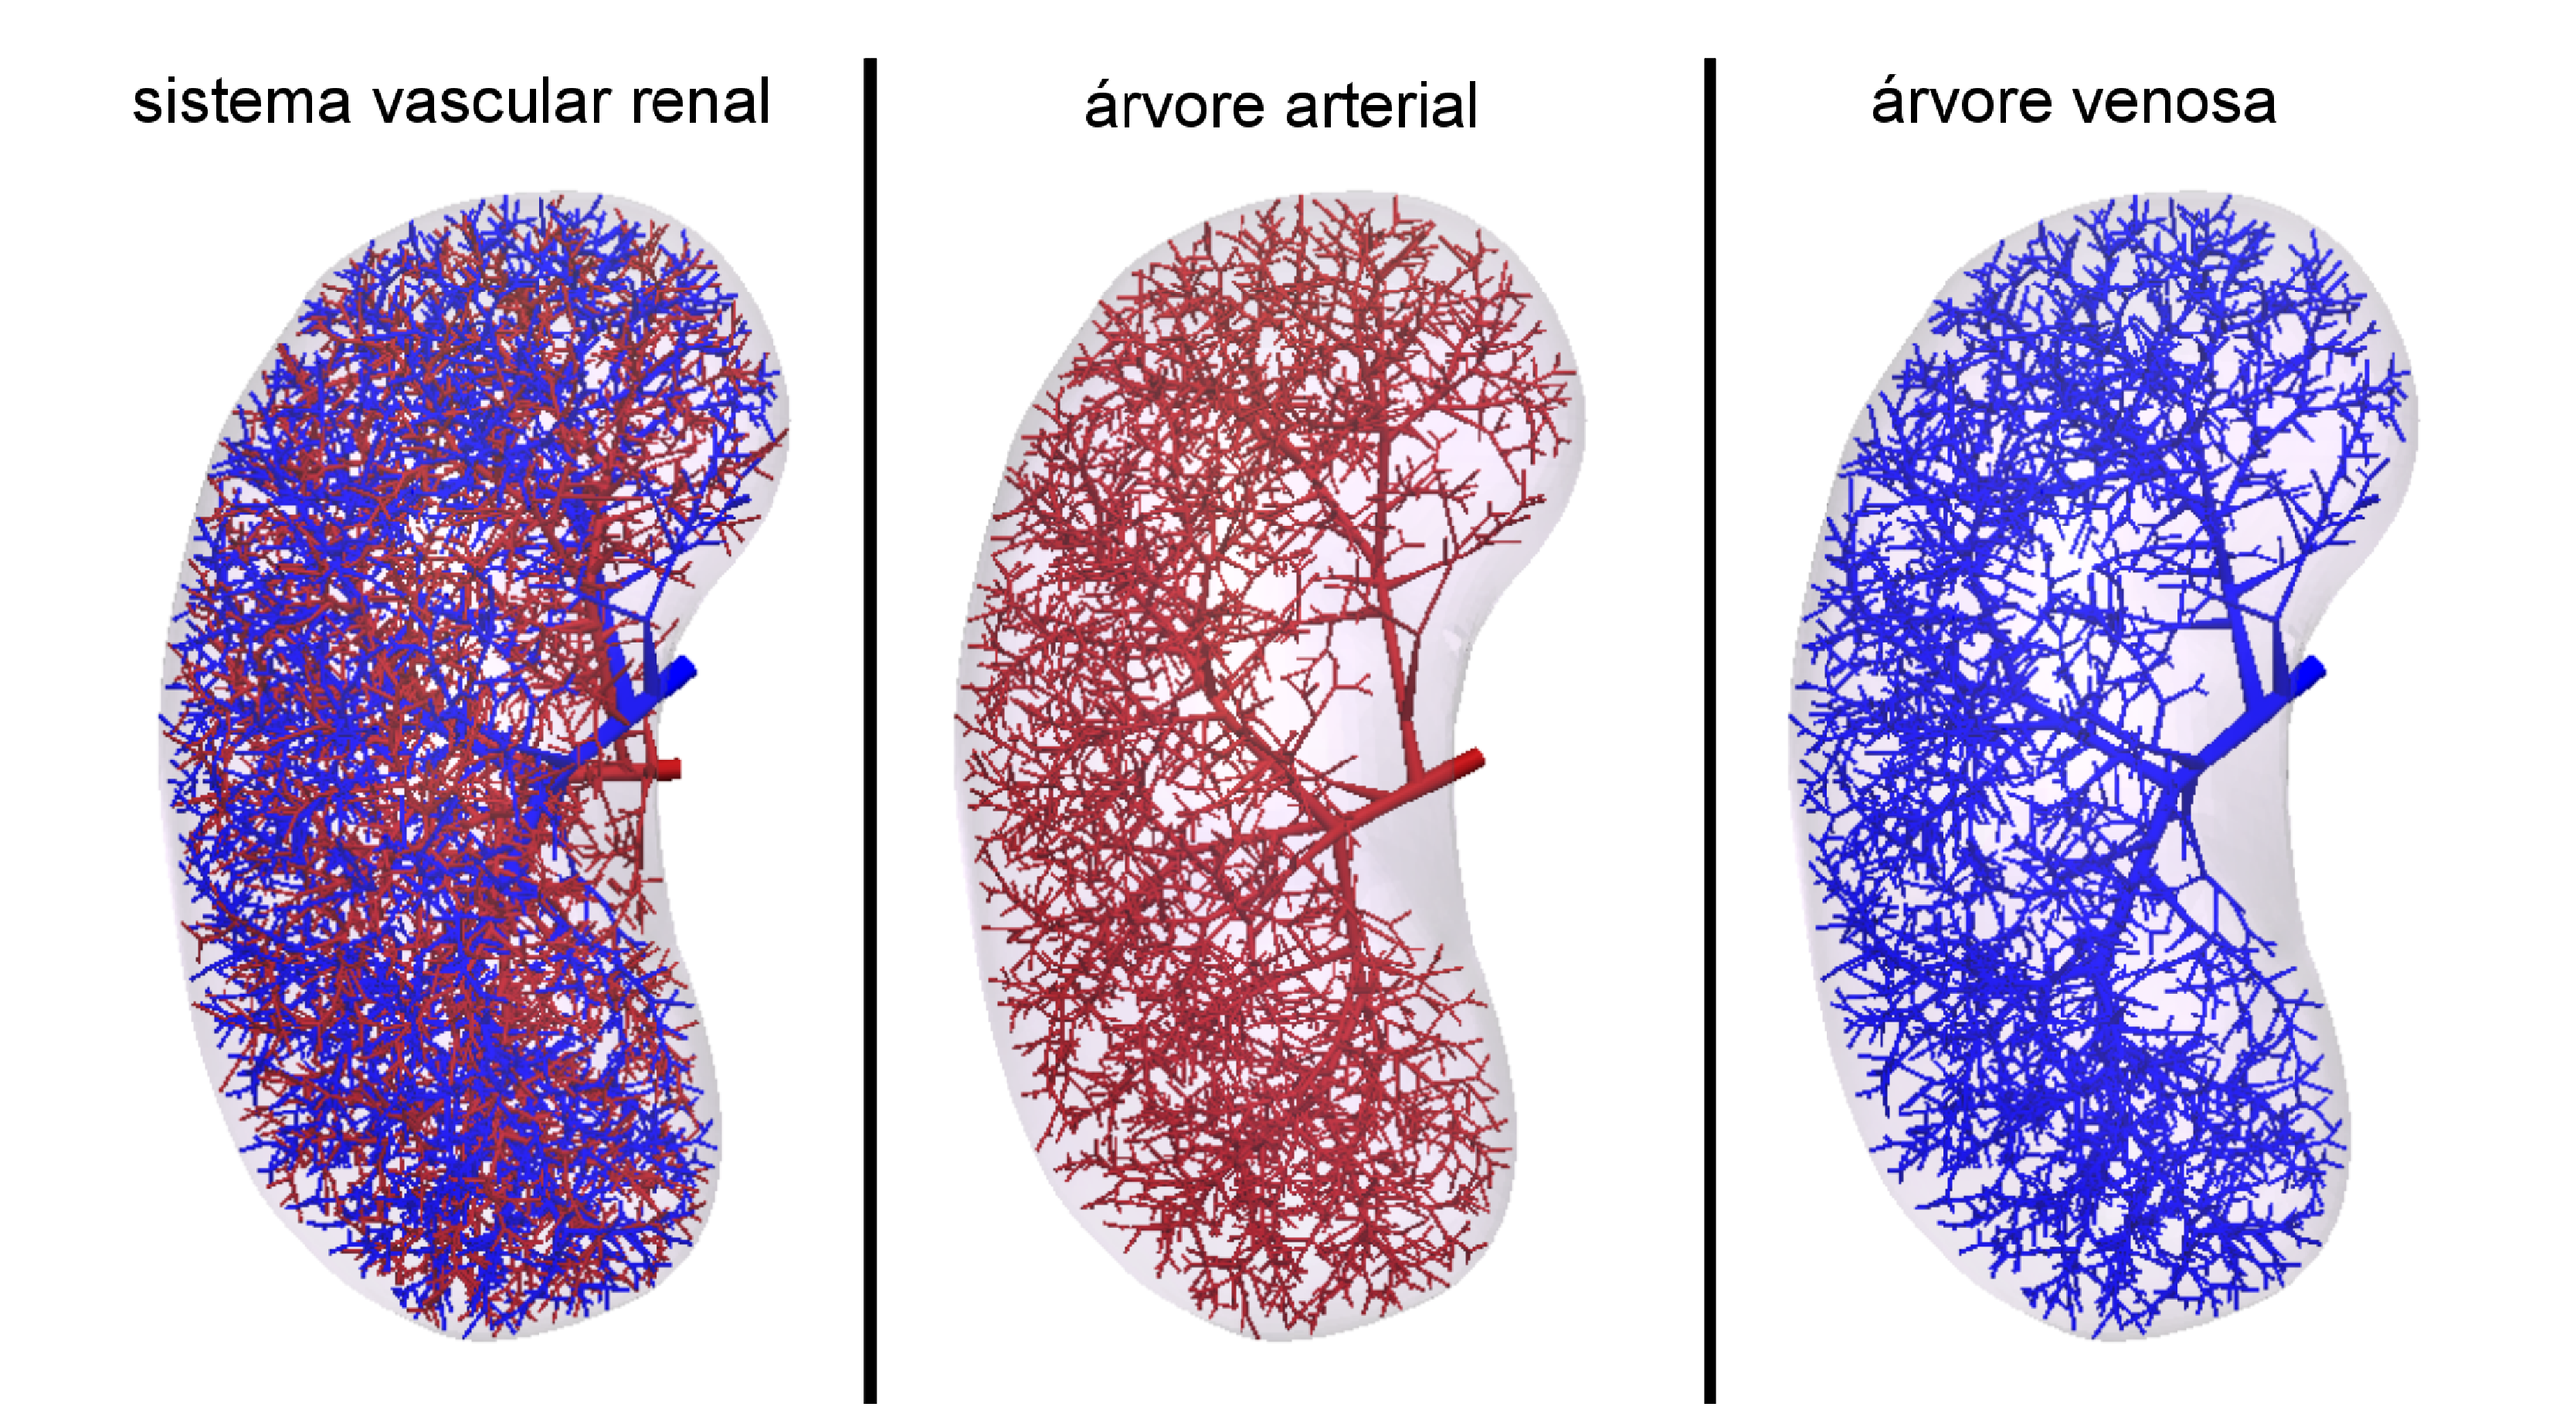
\includegraphics[width=\textwidth]{figuras/modelos-computacionais-de-arvores-circulatorias/DomFix_RimAcoplamentoNaoUniforme.eps}
  \fonte{Queiroz (2018).}
  \label{fig:resRim3DAcopla}
\end{figure}

Na Tabela~\ref{tab:dados-morfometricos-rim}, os resultados morfométricos das árvores arterial e venosa são apresentados. 
Nessa tabela, AA denota a árvore arterial e AV a árvore venosa. A média e o desvio padrão dos resultados 
foram calculados, pois foram gerados 10 modelos do sistema, alterando-se a distribuição dos pontos terminais no 
domínio. Nota-se que o raio do segmento raiz ($r_{iroot}$) do modelo de árvore arterial está consistente com o 
raio de uma artéria renal real, que está entre 2mm e 6mm de acordo com~\cite{Weld2005}. O valor do raio do 
segmento raiz do modelo de árvore venosa está relativamente próximo do valor do raio de uma veia 
renal real, que varia entre 5mm e 7mm conforme~\cite{Satyapal2019}. Como esperado, o raio do segmento raiz 
e o volume intravascular ($V$) são maiores para as árvores venosas do que aqueles das árvores arteriais.

É apresentado ainda na Tabela~\ref{tab:dados-morfometricos-rim} o número 
máximo de níveis de bifurcação ($n_{\max}$), isto é, o número máximo de 
pontos de bifurcação partindo do segmento raiz até o segmento terminal mais distante
na árvore. A Figura~\ref{fig:nivel-de-bifurcacao} ilustra o cálculo do nível de bifurcação
em uma árvore genérica.

\begin{figure}[!htb]
  \centering
  \captiondelim{: }
  \caption{Exemplo do cálculo do nível de bifurcação.}
  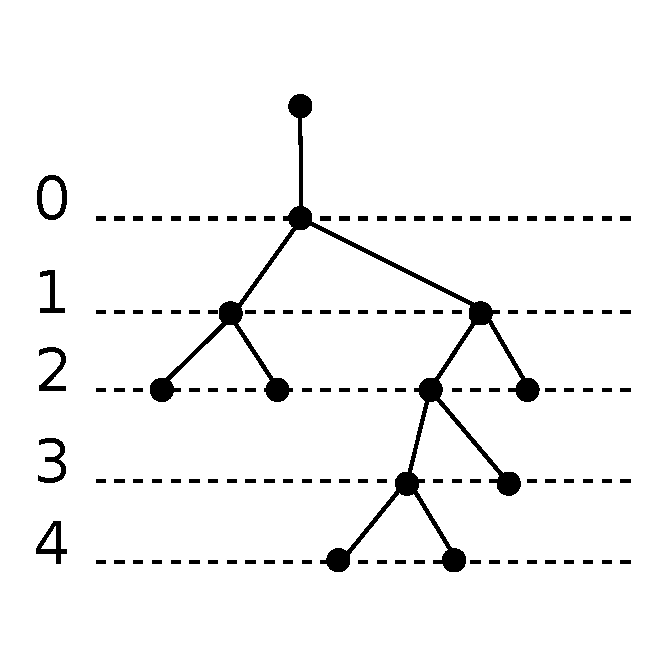
\includegraphics[width=0.25\textwidth]{figuras/modelos-computacionais-de-arvores-circulatorias/nivel-de-bifurcacao.pdf}
  \fonte{Queiroz (2018).}
  \label{fig:nivel-de-bifurcacao}
\end{figure}

\begin{table}[!htb]
\centering
\captiondelim{: }
\caption{Propriedades morfométricas do sistema vascular renal gerado.}
\begin{tabular}{|c|c|c|c|c|c|}
  \hline 
 Árv.  & $r_{iroot}$ (mm) & $r_{\min}$ (mm) & $V$ (mm$^3$) & $n_{\max}$ \\
\hline
AA & $2,0900 \pm 0,0019$ & $0,0138 \pm 0,0017$ & $720,0206 \pm  6,6782 $ & $44 \pm 2$ \\
AV & $4,0862 \pm 0,0106$ & $0,0289 \pm 0,0031$ & $2797,5518 \pm 23,1052$ & $48 \pm 4$ \\
\hline
\end{tabular}
  \fonte{Queiroz (2018).}
\label{tab:dados-morfometricos-rim}
\end{table}

Na Figura~\ref{fig:CurveMorfometricaRim} são apresentadas as curvas morfométricas que relacionam o diâmetro médio 
do segmento em função de seu nível de bifurcação das árvores arterial 
e venosa do sistema renal gerado pelo Algoritmo~\ref{algo:CCOVenosoArterial}. 
Salienta-se que o decaimento apresentado nas curvas se assemelha 
aos dados experimentais oriundos de corrosão vascular de árvores coronarianas reais~\cite{Zamir1987}.

\begin{figure}[!htb]
  \centering
  \captiondelim{: }
  \caption{Curvas morfométricas que relacionam o diâmetro médio do segmento com seu nível de bifurca\c{c}\~ao
das árvores arterial e venosa do sistema renal.) (a) Árvore arterial. (b) Árvore venosa.}
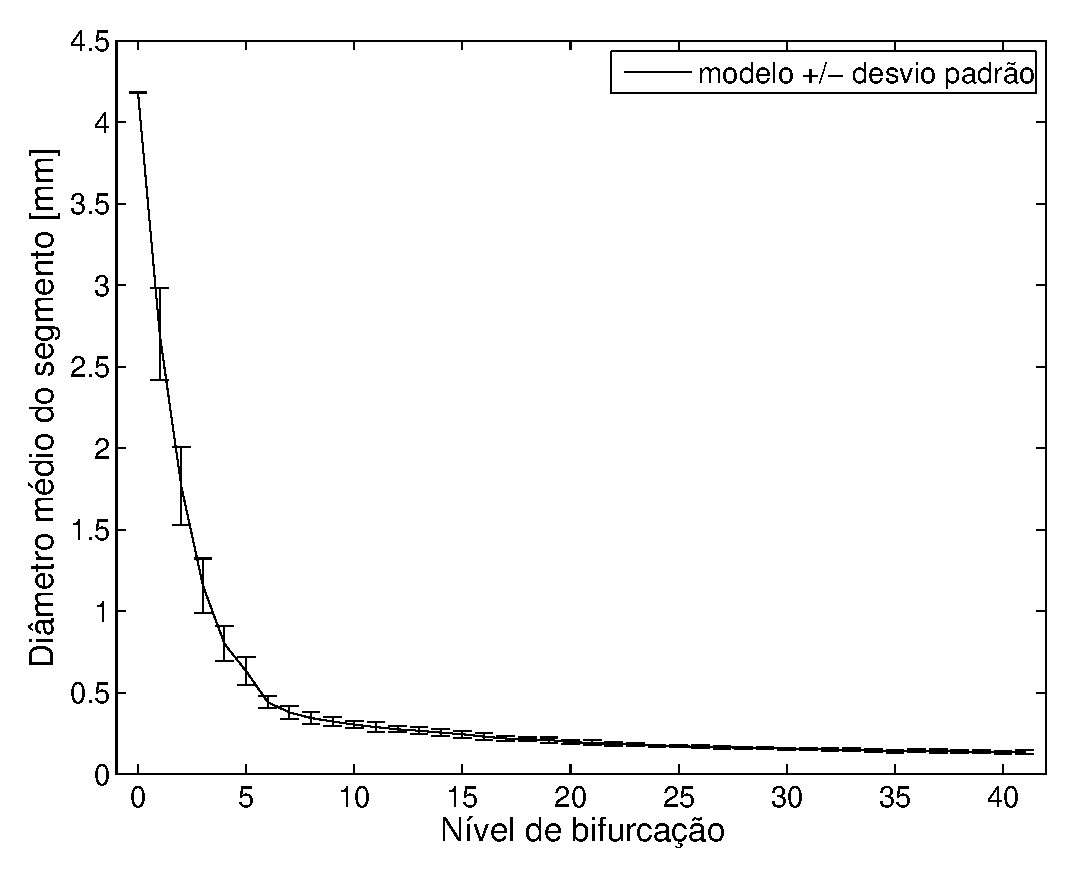
\includegraphics[width=0.49\textwidth]{figuras/modelos-computacionais-de-arvores-circulatorias/res_domfix_nonunif_tree1.eps}
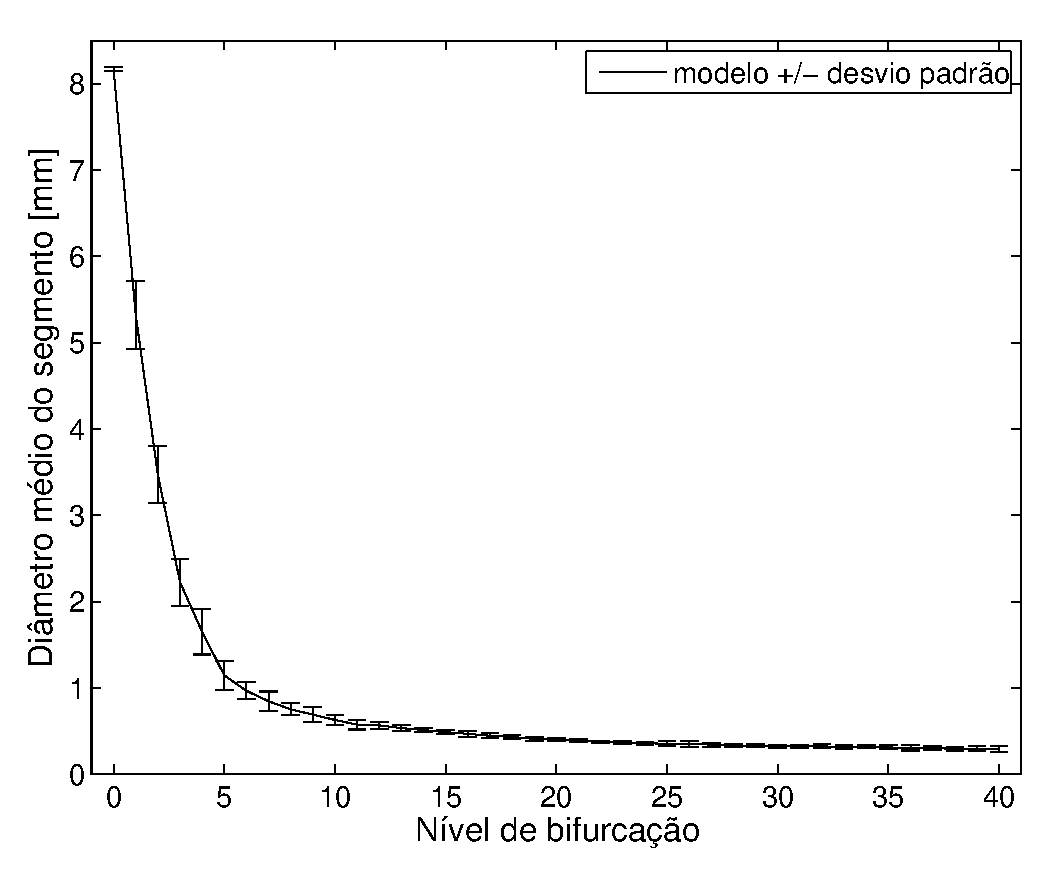
\includegraphics[width=0.49\textwidth]{figuras/modelos-computacionais-de-arvores-circulatorias/res_domfix_nonunif_tree2.eps}

  (a) \hspace{0.5\textwidth} (b)
  \fonte{Queiroz (2018).}
  \label{fig:CurveMorfometricaRim}
\end{figure}

\clearpage

\section{FLORESTAS DE ÁRVORES ARTERIAIS COM COEFICIENTE DE INVASÃO}\label{sec:floresta-invasao-resultados}

Como prova de conceito do Algoritmo~\ref{algo:FlorestaDeArvoresComInvasao}, 
ele foi aplicado em dois domínios de perfusão, sendo um deles bidimensional 
não convexo e o outro tridimensional convexo. O domínio bidimensional não
convexo tem formato de disco, com raio externo de 5 cm e interno de 1,5 cm. 
Já o domínio tridimensional convexo, tem o formato de esfera com raio de 
aproximadamente 2,879 cm (ou seja, para um volume de 100 cm$^3$). Esses 
domínios foram escolhidos de modo a representar a floresta suprindo 
100 $g$ de tecido do miocárdio durante máxima vasodilatação~\cite{Schreiner1993b}.
A Tabela~\ref{tab:parametros-floresta-invasao-2d} apresenta os parâmetros 
usados na execução.

As coordenadas dos pontos 
nesses domínios foram criadas usando o gerador de números aleatórios
dSFMT~\cite{Saito2009}. Ambos os domínios foram ocupados por uma 
floresta com duas árvores ($N_{trees} = 2$) e número total de terminais
igual a 250 ($N_{term} = 250$).
Além disso, os fluxos alvos $q_{targ}^1$ e $q_{targ}^2$, 
respectivamente, referentes às árvores $t = 1$ e $t = 2$, variaram 
conforme indicado na Tabela~\ref{tab:casos-fluxo-duas-arvores}, de tal modo 
que $\dfrac{q_{targ}^1}{q_{targ}^2} = n$, com $n = 1$, 2, \ldots, 10.

No caso do domínio tridimensional (3D), também foram realizados experimentos 
com três árvores ($N_{trees} = 3$), número total de terminais igual a 250 
($N_{term} = 250$) e com fluxos alvos $q_{targ}^1$, $q_{targ}^2$ e $q_{targ}^3$, 
respectivamente, referentes às árvores $t = 1$, $t = 2$ e $t = 3$, variando
conforme indicado na Tabela~\ref{tab:casos-fluxo-tres-arvores}, 
de tal modo que 
$\left(\dfrac{q_{targ}^1}{q_{targ}^2},\, \dfrac{q_{targ}^2}{q_{targ}^3}\right) = (m,\,n)$, 
com $(m,\, n) \in \{1,\, 2,\, 3\}\times \{1,\, 2,\, 3\}$.

Cada um dos casos 
nas Tabelas~\ref{tab:casos-fluxo-duas-arvores} e~\ref{tab:casos-fluxo-tres-arvores} 
foi executado dez vezes, alterando a semente do gerador de números aleatórios em cada execução.

\begin{table}[!htb]
  \centering \captiondelim{: }
  \caption{
    Casos para a distribuição dos fluxos alvos $q_{targ}^1$ e $q_{targ}^2$,
    respectivamente, referentes às árvores $t = 1$ e $t = 2$.
  }
  \begin{tabular}{|c|c|c|c|}
    \hline
    Caso & $q_{targ}^1$ (\%) & $q_{targ}^2$ (\%) \\ \hline
    1 & 50,00 & 50,00 \\ \hline
    2 & 66,70 & 33,30 \\ \hline
    3 & 75,00 & 25,00 \\ \hline
    4 & 80,00 & 20,00 \\ \hline
    5 & 83,40 & 16,60 \\ \hline
    6 & 85,70 & 14,30 \\ \hline
    7 & 87,50 & 12,50 \\ \hline
    8 & 88,90 & 11,10 \\ \hline
    9 & 90,00 & 10,00 \\ \hline
    10 & 90,90 & 9,10\\ \hline
  \end{tabular}
  \fonteAutor{2022}\label{tab:casos-fluxo-duas-arvores}
\end{table}

\begin{table}[!htb]
  \centering \captiondelim{: }
  \caption{
    Casos para a distribuição dos fluxos alvos $q_{targ}^1$, $q_{targ}^2$ e 
    $q_{targ}^3$, respectivamente, referentes às árvores $t = 1$, $t = 2$ e 
    $t = 3$.
  }
  \begin{tabular}{|c|c|c|c|c|}
    \hline
    Caso & $q_{targ}^1$ (\%) & $q_{targ}^2$ (\%) & $q_{targ}^3$ (\%) \\ \hline
    1 & 33,40 & 33,30 & 33,30 \\ \hline
    2 & 40,00 & 40,00 & 20,00 \\ \hline
    3 & 42,90 & 42,70 & 14,40 \\ \hline
    4 & 50,00 & 25,00 & 25,00 \\ \hline
    5 & 57,20 & 28,50 & 14,30 \\ \hline
    6 & 60,00 & 30,00 & 10,00 \\ \hline
    7 & 60,00 & 20,00 & 20,00 \\ \hline
    8 & 66,70 & 22,20 & 11,10 \\ \hline
    9 & 69,20 & 23,10 & 7,70 \\ \hline
  \end{tabular}
  \fonteAutor{2022}\label{tab:casos-fluxo-tres-arvores}
\end{table}

\begin{table}[!htb]
 \centering
 \captiondelim{: }
 \caption{
   Parâmetros usados no Algoritmo~\ref{algo:FlorestaDeArvoresComInvasao}
   em conformidade com os dados da literatura~\cite{Jaquet2019,Karch1999,Schreiner1993b}.}
 \begin{tabular}{|l|l|}
  \hline
  Parâmetro & Valor \\ \hline
  Viscosidade ($\mu$) & $3,6\cdot 10^{-3}$ Pa \\ \hline
  Fluxo de perfusão ($Q_{perf}$) & $8,33$ cm$^3$/s \\ \hline        
  Pressão de perfusão ($p_{perf}$) & $1,333 \cdot 10^4$ Pa ($\approx 100$ mmHg)\\ \hline
  Pressão terminal ($p_{term}$) & 
  \begin{tabular}{c}
    Caso 2D: $8,399 \cdot 10^3$ Pa ($\approx 63$ mmHg). \\
    Caso 3D: $9,599\cdot 10^3$ Pa ($\approx 72$ mmHg).
  \end{tabular}\\\hline
  Expoente de bifurcação ($\gamma$) & 3,0 \\ \hline
  Número de árvores ($N_{trees}$) & 2 \\ \hline
  Número de terminais ($N_{term}$) & 250 \\ \hline
  Número de segmentos vizinhos ($N_{con}$) & 20 \\ \hline
  Coeficiente de invasão ($\alpha$) & 0,75 \\ \hline
  Número de tentativas ($N_{toss}$) & 10 \\ \hline
  Fator de redução ($\beta$) & 0,9 \\ \hline
 \end{tabular}
 \fonteAutor{2022}
 \label{tab:parametros-floresta-invasao-2d}
\end{table}

\clearpage

Os resultados obtidos na execução dos casos estão descritos 
nas Seções~\ref{sec:floresta-com-invasao-caso-2d},
\ ~\ref{sec:floresta-com-invasao-caso-3d} e~\ref{sec:floresta-com-invasao-caso-3arvores-3d}. 
Para analisar o território $T_t$ ocupado pela árvore $t$, 
empregou-se o diagrama de Voronoi usando os pontos $P_i$ 
distais dos segmentos de $t$, conforme~\eqref{def:diagrama-voronoi}. 

Em~\cite{West1997} é apresentado que a massa $M$ da aorta de mamíferos 
e a área $Y$ de sua seção transversal estão relacionadas por uma lei alométrica no
formato:
\begin{equation}
  Y = Y_0 M^\frac{3}{4},
  \label{eq:lei-alometrica-secao-transversal-vs-area}
\end{equation}
onde $Y_0$ é uma constante. Considerando que o raio do segmento raiz de cada árvore $t$ 
seja $r_{iroot,\,t}$ e que o respectivo território ocupado por essa árvore seja $T_t$, 
deseja-se investigar se eles estão relacionados através de alguma lei 
como~\eqref{eq:lei-alometrica-secao-transversal-vs-area}. 

Supondo que as árvores $i$ e $j$ de uma floresta são tais 
que $\dfrac{T_i}{T_j} \neq 1$, deseja-se analisar a existência de um expoente
$b$ tal que:
\begin{eqnarray}
  \begin{cases}
    \pi r_{iroot,\,i}^2 = Y_0T_i^{b}\\
    \pi r_{iroot,\,j}^2 = Y_0T_j^{b}
  \end{cases}\implies
  \dfrac{r_{iroot,\,i}^2}{r_{iroot\,j}^2} = \dfrac{T_i^{b}}{T_j^{b}}
  \implies
  \dfrac{\ln\left(\dfrac{r_{iroot,\,i}}{r_{iroot,\,j}}\right)}{\ln\left(\dfrac{T_i}{T_j}\right)} = \dfrac{b}{2}
  \label{eq:desenvolvimento-lei-alometrica}
\end{eqnarray}

Nota-se que a restrição $\dfrac{T_i}{T_j} \neq 1$ deve ser utilizada 
para que  $\ln\left(\dfrac{T_i}{T_j}\right) \neq 0$ e assim não ocorra uma divisão 
por zero em~\eqref{eq:desenvolvimento-lei-alometrica}. Por praticidade na 
análise dos resultados, nesse trabalho adota-se a convenção:
\begin{equation}
  \delta_{i, j} = \dfrac{\ln\left(\dfrac{r_{iroot,\,i}}{r_{iroot,\,j}}\right)}{\ln\left(\dfrac{T_i}{T_j}\right)}
  \label{eq:lei-alometrica-delta-ij}
\end{equation}

\clearpage

\subsection{Caso bidimensional}\label{sec:floresta-com-invasao-caso-2d}

A Tabela~\ref{tab:resultados-floresta-com-invasao-2d} resume os resultados
das simulações para verificar o fluxo obtido e o território ocupado, em contraste com o 
fluxo alvo fornecido.
Verifica-se que o erro relativo médio entre o fluxo obtido e o fluxo alvo foi 
de $0,018 \pm 0,024$. Isso representa um erro inferior a $2\%$. 
Além disso, a relação entre o fluxo obtido e o território ocupado estão correlacionados com um
coeficiente de $0,998$. 

A Tabela~\ref{tab:resultados-lei-alometrica-floresta-com-invasao-2d} apresenta os resultados 
para verificar a lei alométrica~\eqref{eq:desenvolvimento-lei-alometrica}. Destaca-se que os valores
de $\delta_{1, 2}$ dessa lei ficaram próximos de $0,375$.

As Figuras~\ref{fig:ilustracoes-floresta-com-invasao-2d-parte1} e~\ref{fig:ilustracoes-floresta-com-invasao-2d-parte2} 
ilustram as florestas obtidas para os dez casos de distribuição de fluxo conforme 
a Tabela~\ref{tab:casos-fluxo-duas-arvores}. 
Em cada caso foi considerada a mesma semente do gerador dSFMT. 
Em cada floresta a cor vermelha foi utilizada 
para ilustrar a árvore 1 e a cor verde a árvore 2.
Já nas Figuras~\ref{fig:diametro-medio-floresta-com-invasao-caso-2d-parte1},\ 
~\ref{fig:diametro-medio-floresta-com-invasao-caso-2d-parte2},\ 
~\ref{fig:diametro-medio-floresta-com-invasao-caso-2d-parte3}\ 
e~\ref{fig:diametro-medio-floresta-com-invasao-caso-2d-parte4} são apresentadas 
as curvas morfométricas que relacionam o diâmetro médio 
do segmento em função de seu nível de bifurcação. Nota-se que essas curvas apresentam
o mesmo comportamento de decaimento conforme~\cite{Karch1999}.

\clearpage

\begin{table}[!htb]
  \centering
  \captiondelim{: }
  \caption{Resultados obtidos com a construção de florestas de árvores circulatórias 
empregando o Algoritmo~\ref{algo:FlorestaDeArvoresComInvasao} com as modificações propostas.}
\begin{tabular}{|c|c|c|c|c|}
\hline
Caso & Fluxo alvo (\%) & Fluxo obtido (\%) & Território (\%) & Volume (\%) \\ \hline
\multirow{2}{*}{1} & \multirow{2}{*}{\begin{tabular}[c]{c} 50,00 \\ 50,00\end{tabular}} & \multirow{2}{*}{\begin{tabular}[c]{c} 53,64 \\ 46,36\end{tabular}} & \multirow{2}{*}{\begin{tabular}[c]{c} $53,35 \pm 7,26$ \\ $46,65 \pm 7,26$\end{tabular}} & \multirow{2}{*}{\begin{tabular}[c]{c} $47,37 \pm 5,84$ \\ $52,63 \pm 5,84$\end{tabular}} \\
 & & & & \\ \hline
\multirow{2}{*}{2} & \multirow{2}{*}{\begin{tabular}[c]{c} 66,67 \\ 33,33\end{tabular}} & \multirow{2}{*}{\begin{tabular}[c]{c} 66,80 \\ 33,20\end{tabular}} & \multirow{2}{*}{\begin{tabular}[c]{c} $66,80 \pm 1,11$ \\ $33,20 \pm 1,11$\end{tabular}} & \multirow{2}{*}{\begin{tabular}[c]{c} $77,73 \pm 0,79$ \\ $22,27 \pm 0,79$\end{tabular}} \\
 & & & & \\ \hline
\multirow{2}{*}{3} & \multirow{2}{*}{\begin{tabular}[c]{c} 75,00 \\ 25,00\end{tabular}} & \multirow{2}{*}{\begin{tabular}[c]{c} 75,20 \\ 24,80\end{tabular}} & \multirow{2}{*}{\begin{tabular}[c]{c} $78,27 \pm 1,10$ \\ $21,73 \pm 1,10$\end{tabular}} & \multirow{2}{*}{\begin{tabular}[c]{c} $87,76 \pm 0,44$ \\ $12,24 \pm 0,44$\end{tabular}} \\
 & & & & \\ \hline
\multirow{2}{*}{4} & \multirow{2}{*}{\begin{tabular}[c]{c} 80,00 \\ 20,00\end{tabular}} & \multirow{2}{*}{\begin{tabular}[c]{c} 80,40 \\ 19,60\end{tabular}} & \multirow{2}{*}{\begin{tabular}[c]{c} $84,61 \pm 1,17$ \\ $15,39 \pm 1,17$\end{tabular}} & \multirow{2}{*}{\begin{tabular}[c]{c} $92,20 \pm 0,31$ \\ $7,80 \pm 0,31$\end{tabular}} \\
 & & & & \\ \hline
\multirow{2}{*}{5} & \multirow{2}{*}{\begin{tabular}[c]{c} 83,33 \\ 16,67\end{tabular}} & \multirow{2}{*}{\begin{tabular}[c]{c} 83,60 \\ 16,40\end{tabular}} & \multirow{2}{*}{\begin{tabular}[c]{c} $88,35 \pm 1,79$ \\ $11,65 \pm 1,79$\end{tabular}} & \multirow{2}{*}{\begin{tabular}[c]{c} $94,70 \pm 0,43$ \\ $5,30 \pm 0,43$\end{tabular}} \\
 & & & & \\ \hline
\multirow{2}{*}{6} & \multirow{2}{*}{\begin{tabular}[c]{c} 85,71 \\ 14,29\end{tabular}} & \multirow{2}{*}{\begin{tabular}[c]{c} 86,00 \\ 14,00\end{tabular}} & \multirow{2}{*}{\begin{tabular}[c]{c} $89,78 \pm 1,52$ \\ $10,22 \pm 1,52$\end{tabular}} & \multirow{2}{*}{\begin{tabular}[c]{c} $95,88 \pm 0,49$ \\ $4,12 \pm 0,49$\end{tabular}} \\
 & & & & \\ \hline
\multirow{2}{*}{7} & \multirow{2}{*}{\begin{tabular}[c]{c} 87,50 \\ 12,50\end{tabular}} & \multirow{2}{*}{\begin{tabular}[c]{c} 87,60 \\ 12,40\end{tabular}} & \multirow{2}{*}{\begin{tabular}[c]{c} $92,45 \pm 0,72$ \\ $7,55 \pm 0,72$\end{tabular}} & \multirow{2}{*}{\begin{tabular}[c]{c} $97,00 \pm 0,19$ \\ $3,00 \pm 0,19$\end{tabular}} \\
 & & & & \\ \hline
\multirow{2}{*}{8} & \multirow{2}{*}{\begin{tabular}[c]{c} 88,89 \\ 11,11\end{tabular}} & \multirow{2}{*}{\begin{tabular}[c]{c} 89,20 \\ 10,80\end{tabular}} & \multirow{2}{*}{\begin{tabular}[c]{c} $93,94 \pm 1,29$ \\ $6,06 \pm 1,29$\end{tabular}} & \multirow{2}{*}{\begin{tabular}[c]{c} $97,66 \pm 0,32$ \\ $2,34 \pm 0,32$\end{tabular}} \\
 & & & & \\ \hline
\multirow{2}{*}{9} & \multirow{2}{*}{\begin{tabular}[c]{c} 90,00 \\ 10,00\end{tabular}} & \multirow{2}{*}{\begin{tabular}[c]{c} 90,40 \\ 9,60\end{tabular}} & \multirow{2}{*}{\begin{tabular}[c]{c} $94,67 \pm 0,96$ \\ $5,33 \pm 0,96$\end{tabular}} & \multirow{2}{*}{\begin{tabular}[c]{c} $98,04 \pm 0,31$ \\ $1,96 \pm 0,31$\end{tabular}} \\
 & & & & \\ \hline
\multirow{2}{*}{10} & \multirow{2}{*}{\begin{tabular}[c]{c} 90,91 \\ 9,09\end{tabular}} & \multirow{2}{*}{\begin{tabular}[c]{c} 91,20 \\ 8,80\end{tabular}} & \multirow{2}{*}{\begin{tabular}[c]{c} $96,03 \pm 0,48$ \\ $3,97 \pm 0,48$\end{tabular}} & \multirow{2}{*}{\begin{tabular}[c]{c} $98,59 \pm 0,21$ \\ $1,41 \pm 0,21$\end{tabular}} \\
 & & & & \\ \hline
\end{tabular}
  \fonteAutor{2022}
  \label{tab:resultados-floresta-com-invasao-2d}
\end{table}

\begin{table}[!htb]
  \centering
  \captiondelim{: }
  \caption{Comparativo entre razão $\dfrac{r_{iroot, 1}}{r_{iroot, 2}}$ e $\dfrac{T_1}{T_2}$ 
  em um domínio bidimensional não convexo aplicando o Algoritmo~\ref{algo:FlorestaDeArvoresComInvasao}.}
\begin{tabular}{|c|c|c|c|}
\hline
Caso & $\textrm{mean}\left(\dfrac{r_{iroot, 1}}{r_{iroot, 2}}\right)\pm \textrm{std}$ & $\textrm{mean}\left(\dfrac{T_1}{T_2}\right) \pm \textrm{std}$ & $\textrm{mean}\left(\delta_{1,2}\right) \pm \textrm{std}$ \\ \hline
1 & $0,9839 \pm 0,0352$ & $1,1937 \pm 0,3211$ & -- \\ \hline
2 & $1,3863 \pm 0,0081$ & $2,0152 \pm 0,0979$ & $0,4690 \pm 0,0296$ \\ \hline
3 & $1,6778 \pm 0,0122$ & $3,6149 \pm 0,2450$ & $0,4043 \pm 0,0190$ \\ \hline
4 & $1,9163 \pm 0,0103$ & $5,5343 \pm 0,4930$ & $0,3822 \pm 0,0221$ \\ \hline
5 & $2,1451 \pm 0,0226$ & $7,7747 \pm 1,2557$ & $0,3770 \pm 0,0294$ \\ \hline
6 & $2,3243 \pm 0,0370$ & $8,9945 \pm 1,3939$ & $0,3879 \pm 0,0251$ \\ \hline
7 & $2,5213 \pm 0,0237$ & $12,3681 \pm 1,2097$ & $0,3690 \pm 0,0147$ \\ \hline
8 & $2,6930 \pm 0,0478$ & $16,1844 \pm 3,2879$ & $0,3605 \pm 0,0248$ \\ \hline
9 & $2,8470 \pm 0,0506$ & $18,3026 \pm 3,0182$ & $0,3628 \pm 0,0188$ \\ \hline
10 & $3,0450 \pm 0,0524$ & $24,5587 \pm 2,9839$ & $0,3490 \pm 0,0094$ \\ \hline
\end{tabular}
  \fonteAutor{2022}
  \label{tab:resultados-lei-alometrica-floresta-com-invasao-2d}
\end{table}

\clearpage

\begin{figure}[!htb]
  \centering
  \captiondelim{: }
\caption{Florestas com duas árvores arteriais construídas com diferentes fluxos alvo (árvore 1 em vermelho -- árvore 2 em verde): 
  (a) 50\%--50\%; (b) 66,7\%--33,3\%;  (c) 75\%--25\%;  (d) 80\%--20\%;  (e) 83,33\%--16,67\%.}

  \subfloat[]{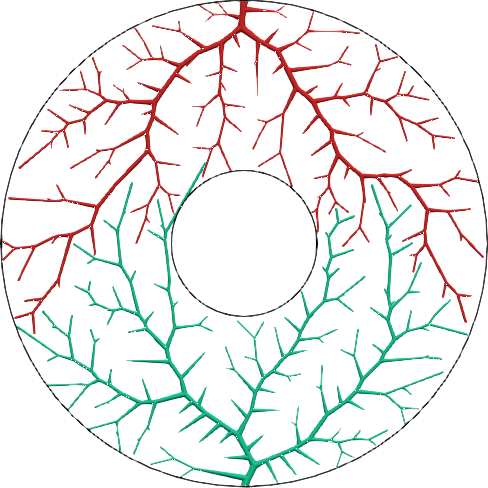
\includegraphics[scale=0.35]{figuras/floresta-com-coeficiente-de-invasao/2D/disco/floresta-500-500.png}}
  \hspace{12pt}
  \subfloat[]{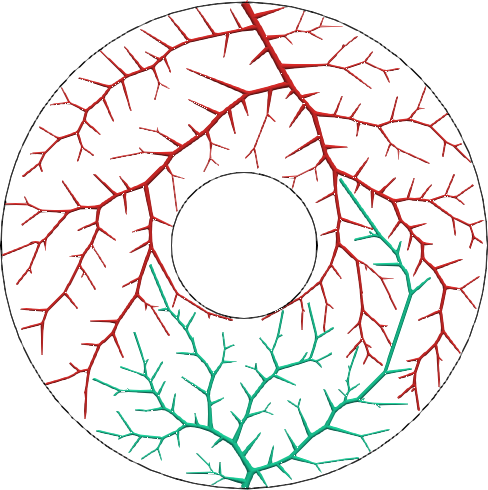
\includegraphics[scale=0.35]{figuras/floresta-com-coeficiente-de-invasao/2D/disco/floresta-667-333.png}}

  \subfloat[]{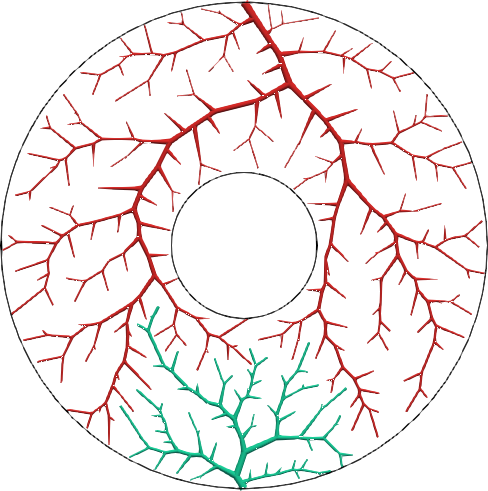
\includegraphics[scale=0.35]{figuras/floresta-com-coeficiente-de-invasao/2D/disco/floresta-750-250.png}}
  \hspace{12pt}
  \subfloat[]{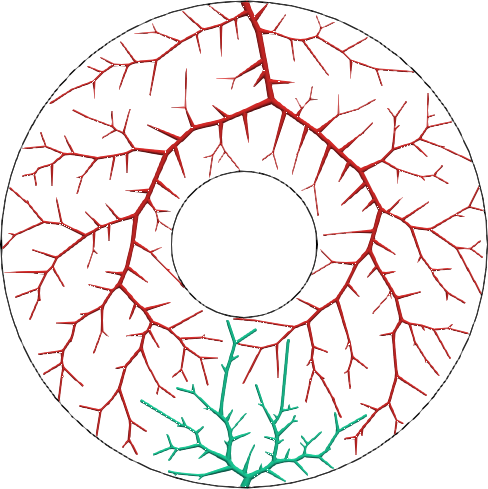
\includegraphics[scale=0.35]{figuras/floresta-com-coeficiente-de-invasao/2D/disco/floresta-800-200.png}}

  \subfloat[]{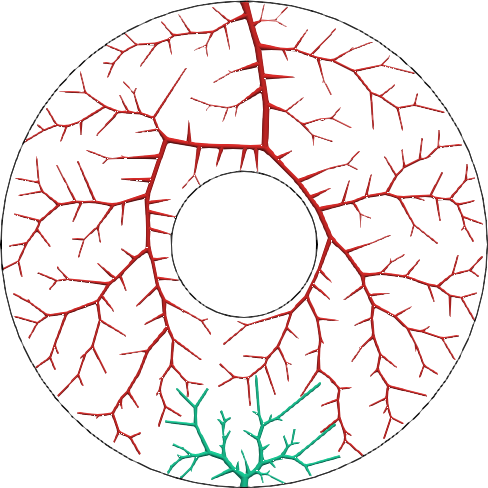
\includegraphics[scale=0.35]{figuras/floresta-com-coeficiente-de-invasao/2D/disco/floresta-834-166.png}}

  \fonteAutor{2022}
  \label{fig:ilustracoes-floresta-com-invasao-2d-parte1}
\end{figure}

\begin{figure}[!htb]
  \centering
  \captiondelim{: }
  \caption{Florestas com duas árvores arteriais construídas com diferentes fluxos alvo (árvore 1 em vermelho -- árvore 2 em verde): 
  (a) 85,71\%--14,29\%; (b) 87,5\%--12,5\%;  (c) 88,89\%--11,11\%;  (d) 90\%--10\%;  (e) 90,91\%--9,09\%.}
  
  \subfloat[]{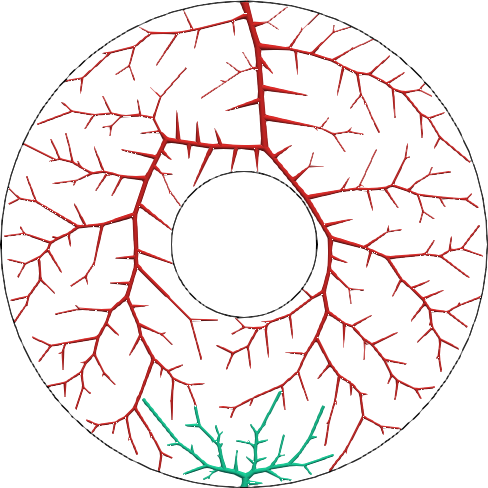
\includegraphics[scale=0.35]{figuras/floresta-com-coeficiente-de-invasao/2D/disco/floresta-857-143.png}}
  \hspace{12pt}
  \subfloat[]{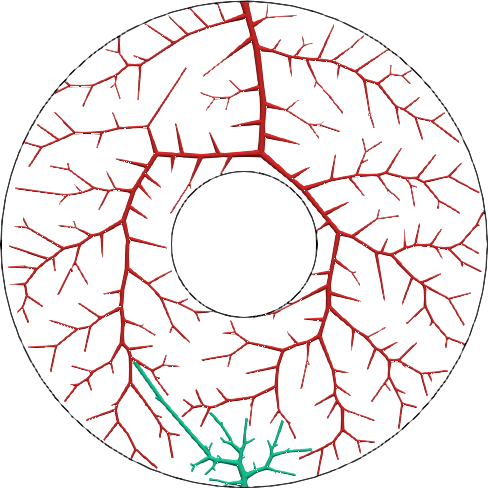
\includegraphics[scale=0.35]{figuras/floresta-com-coeficiente-de-invasao/2D/disco/floresta-875-125.png}}

  \subfloat[]{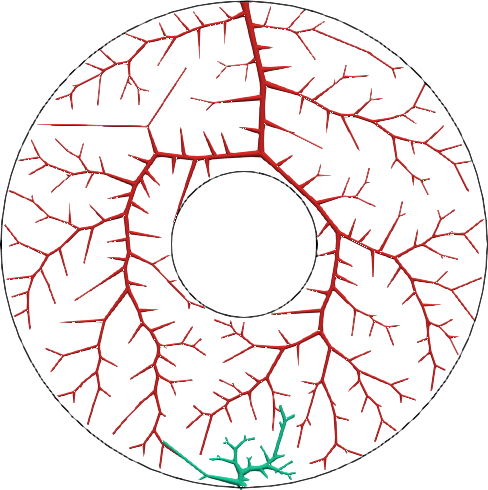
\includegraphics[scale=0.35]{figuras/floresta-com-coeficiente-de-invasao/2D/disco/floresta-889-111.png}}
  \hspace{12pt}
  \subfloat[]{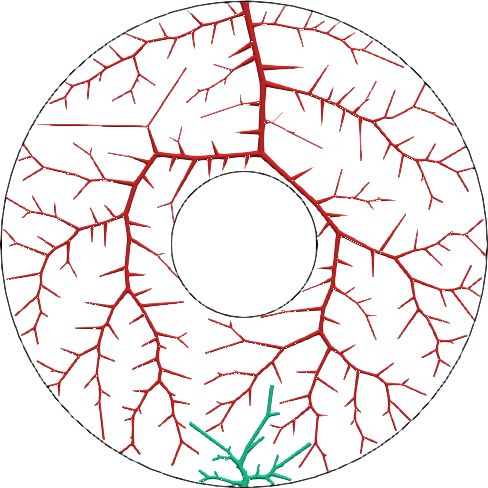
\includegraphics[scale=0.35]{figuras/floresta-com-coeficiente-de-invasao/2D/disco/floresta-900-100.png}}

  \subfloat[]{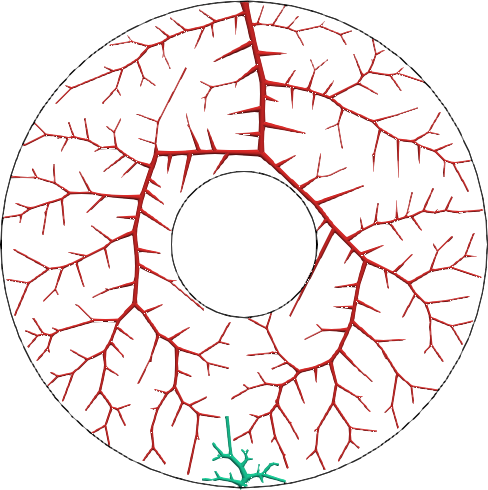
\includegraphics[scale=0.35]{figuras/floresta-com-coeficiente-de-invasao/2D/disco/floresta-909-91.png}}
  \fonteAutor{2022}
  \label{fig:ilustracoes-floresta-com-invasao-2d-parte2}
\end{figure}

\clearpage

\begin{figure}[!htb]
  \centering
  \captiondelim{: }
  \caption{Diâmetro médio do segmento em função de seu nível de bifurcação. 
  Florestas com duas árvores arteriais construídas com diferentes fluxos alvo: 
  (a), (b) Caso 1 (50\%--50\%); (c), (d) Caso 2 (66,7\%--33,3\%);  (e), (f) Caso 3 (75\%--25\%).}
  
  \subfloat[]{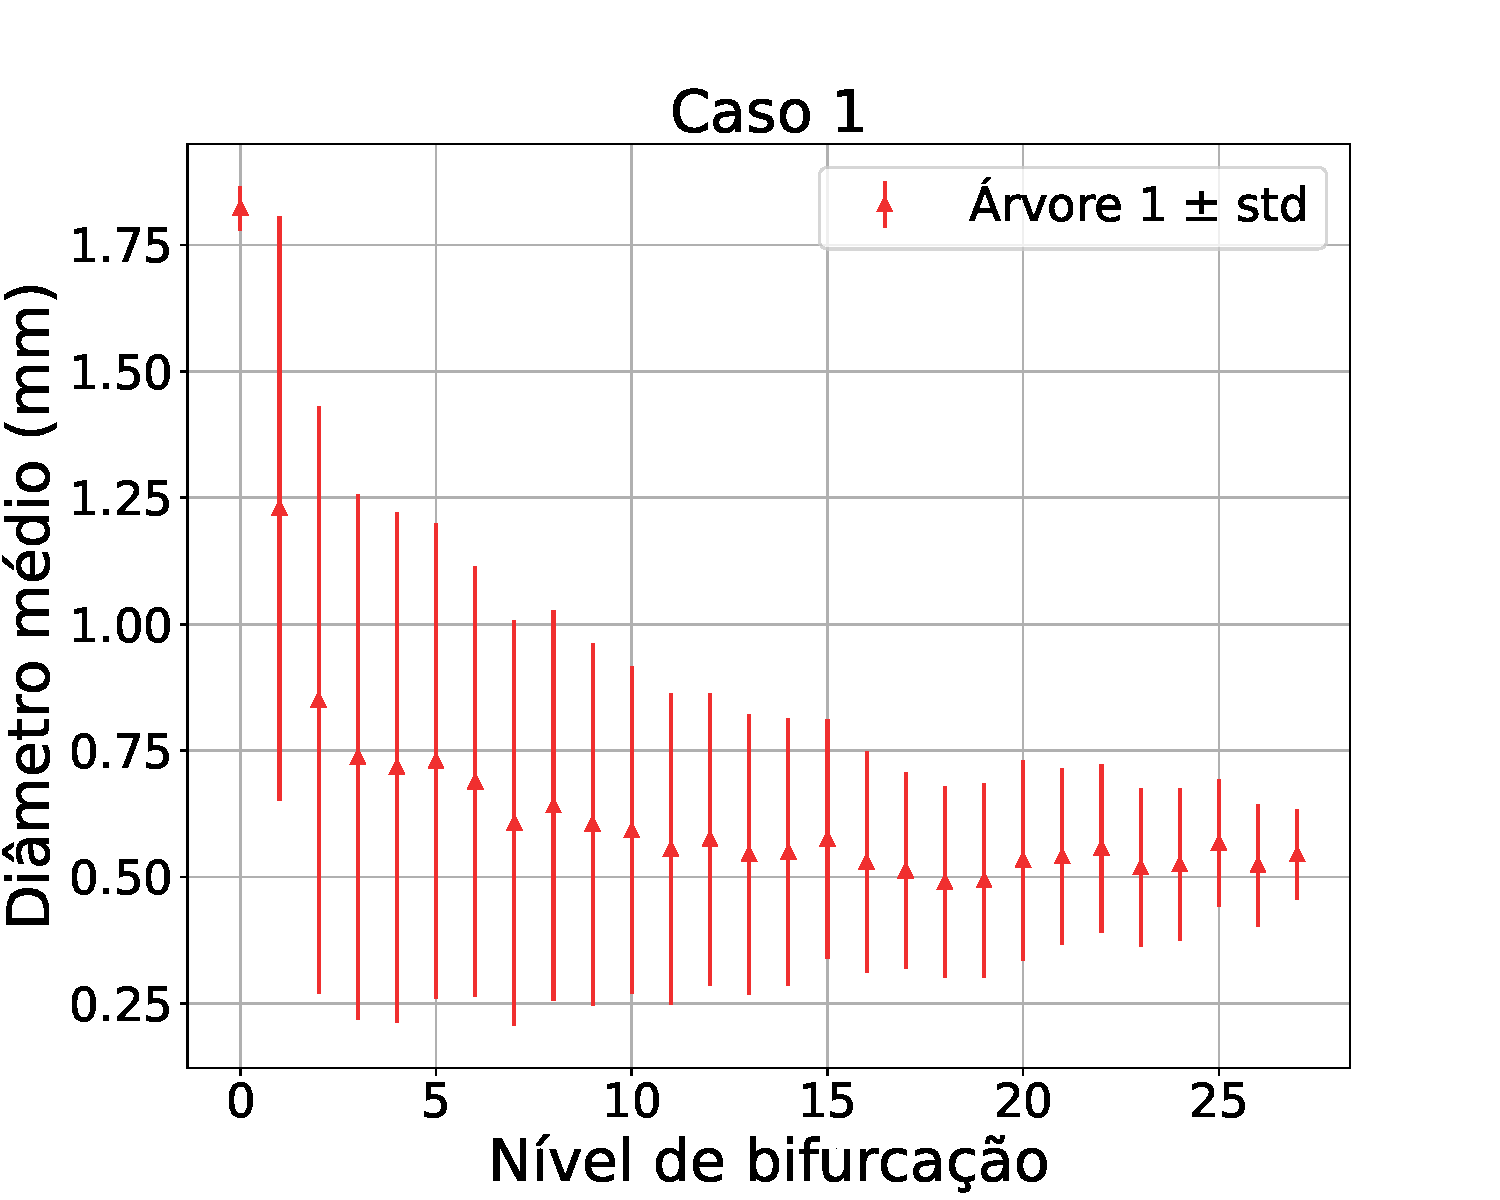
\includegraphics[scale=0.3]{figuras/floresta-com-coeficiente-de-invasao/2D/disco/duas-arvores-diametro-medio-500-500-tree-1.pdf}}
  \hspace{12pt}
  \subfloat[]{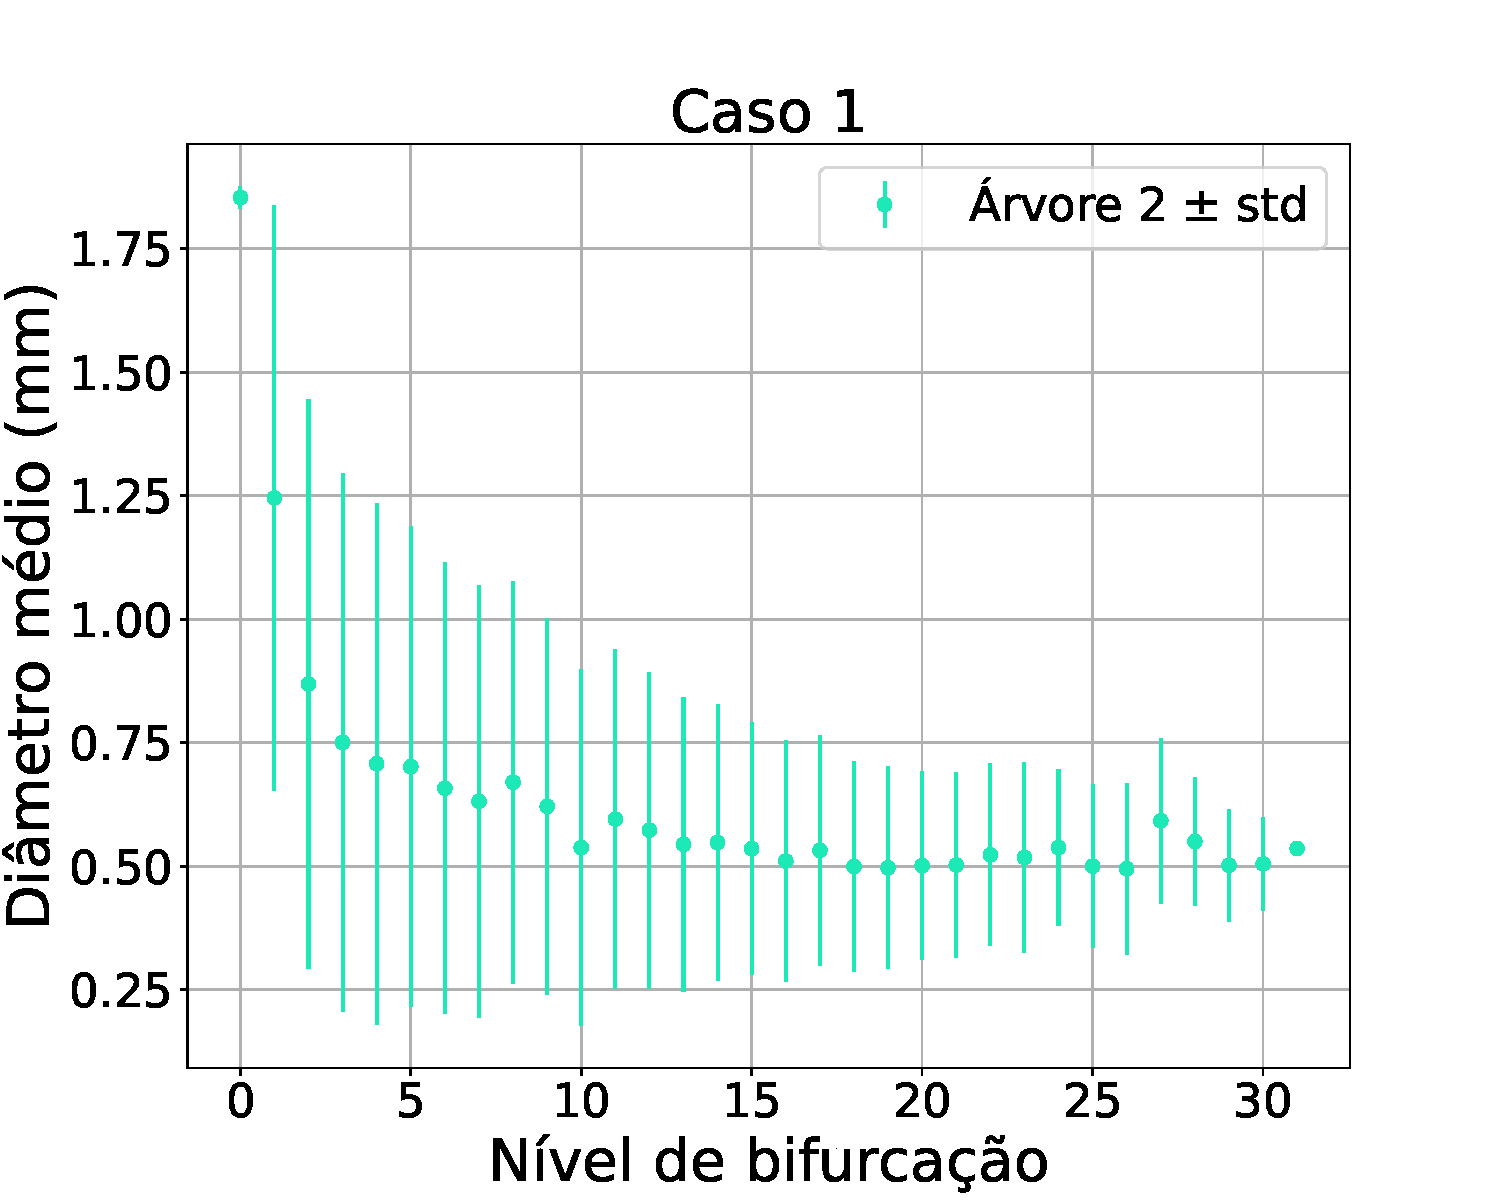
\includegraphics[scale=0.3]{figuras/floresta-com-coeficiente-de-invasao/2D/disco/duas-arvores-diametro-medio-500-500-tree-2.pdf}}

  \subfloat[]{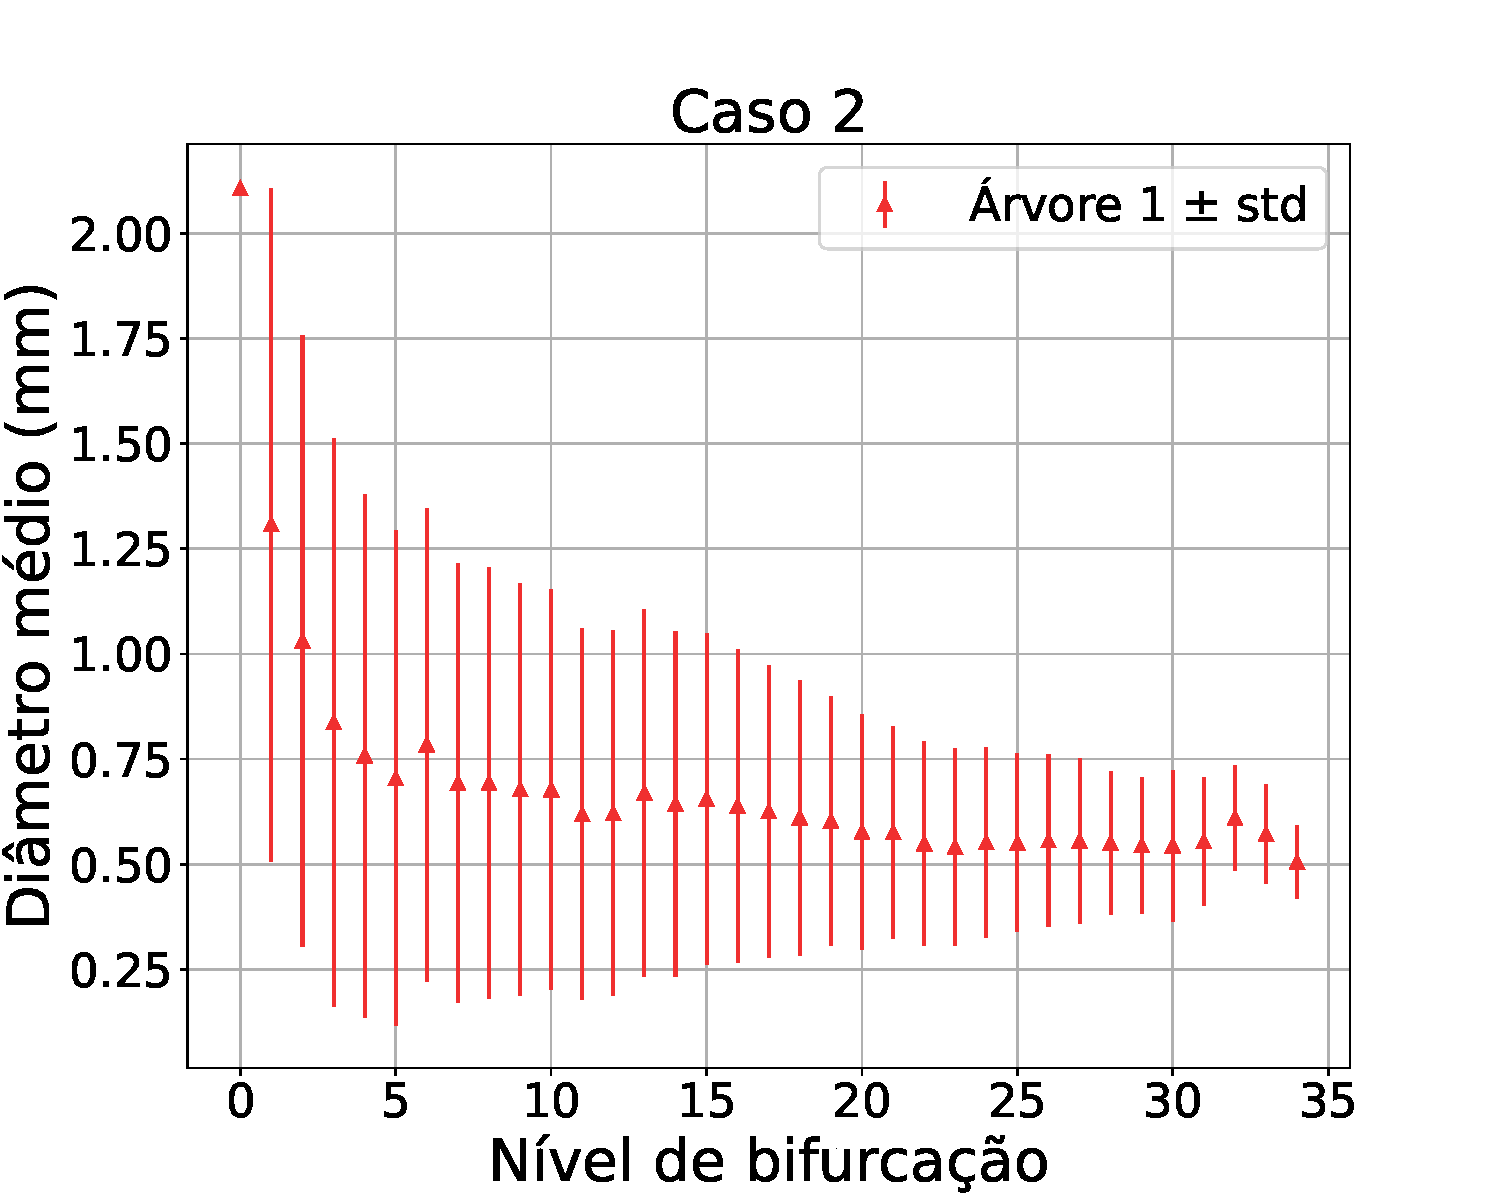
\includegraphics[scale=0.3]{figuras/floresta-com-coeficiente-de-invasao/2D/disco/duas-arvores-diametro-medio-667-333-tree-1.pdf}}
  \hspace{12pt}
  \subfloat[]{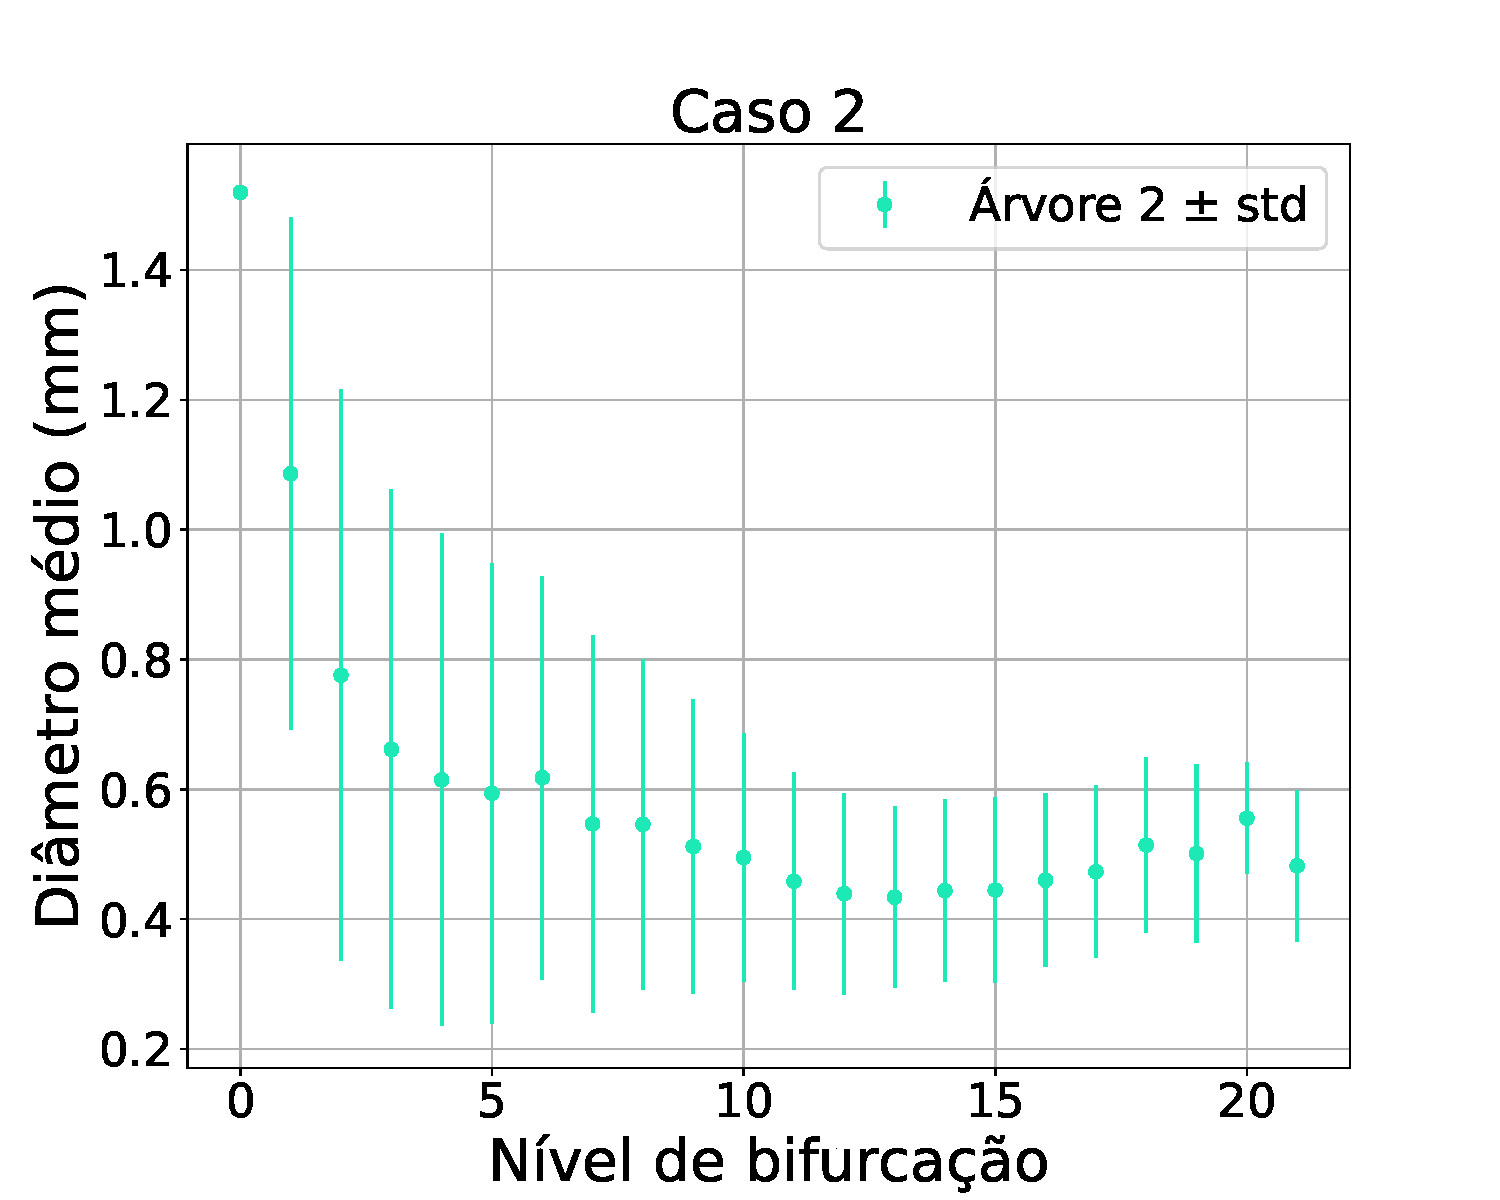
\includegraphics[scale=0.3]{figuras/floresta-com-coeficiente-de-invasao/2D/disco/duas-arvores-diametro-medio-667-333-tree-2.pdf}} 

  \subfloat[]{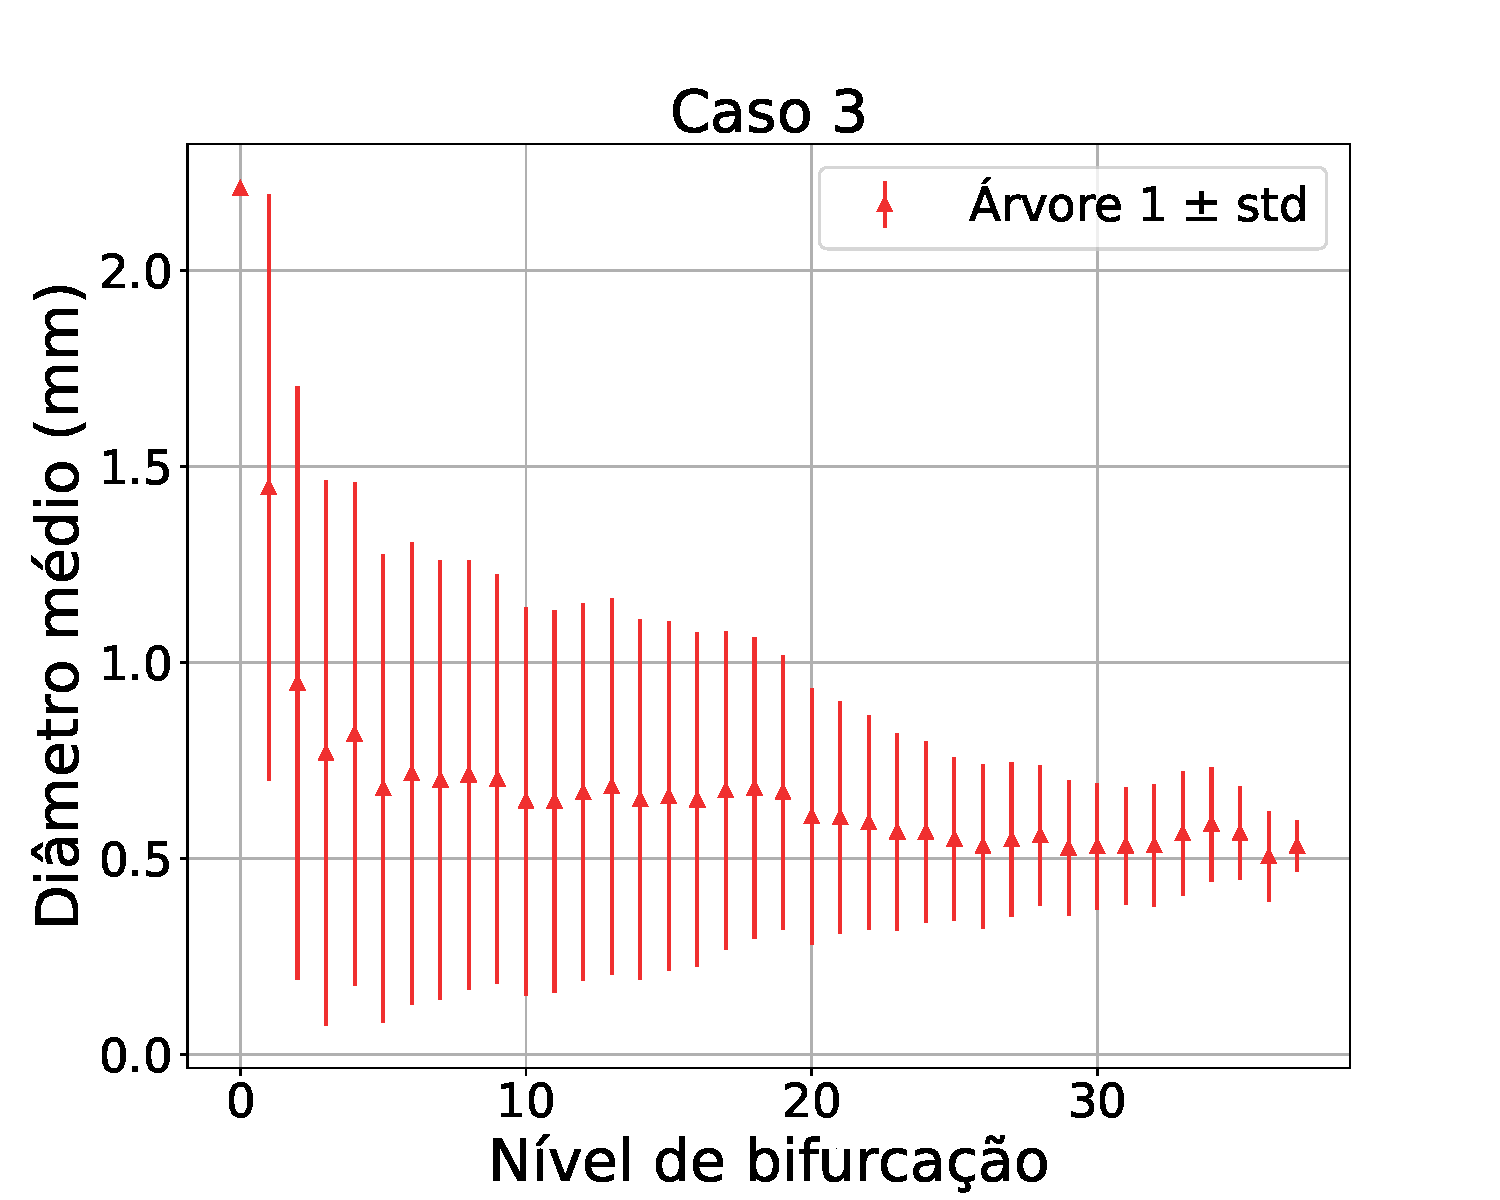
\includegraphics[scale=0.3]{figuras/floresta-com-coeficiente-de-invasao/2D/disco/duas-arvores-diametro-medio-750-250-tree-1.pdf}}
  \hspace{12pt}
  \subfloat[]{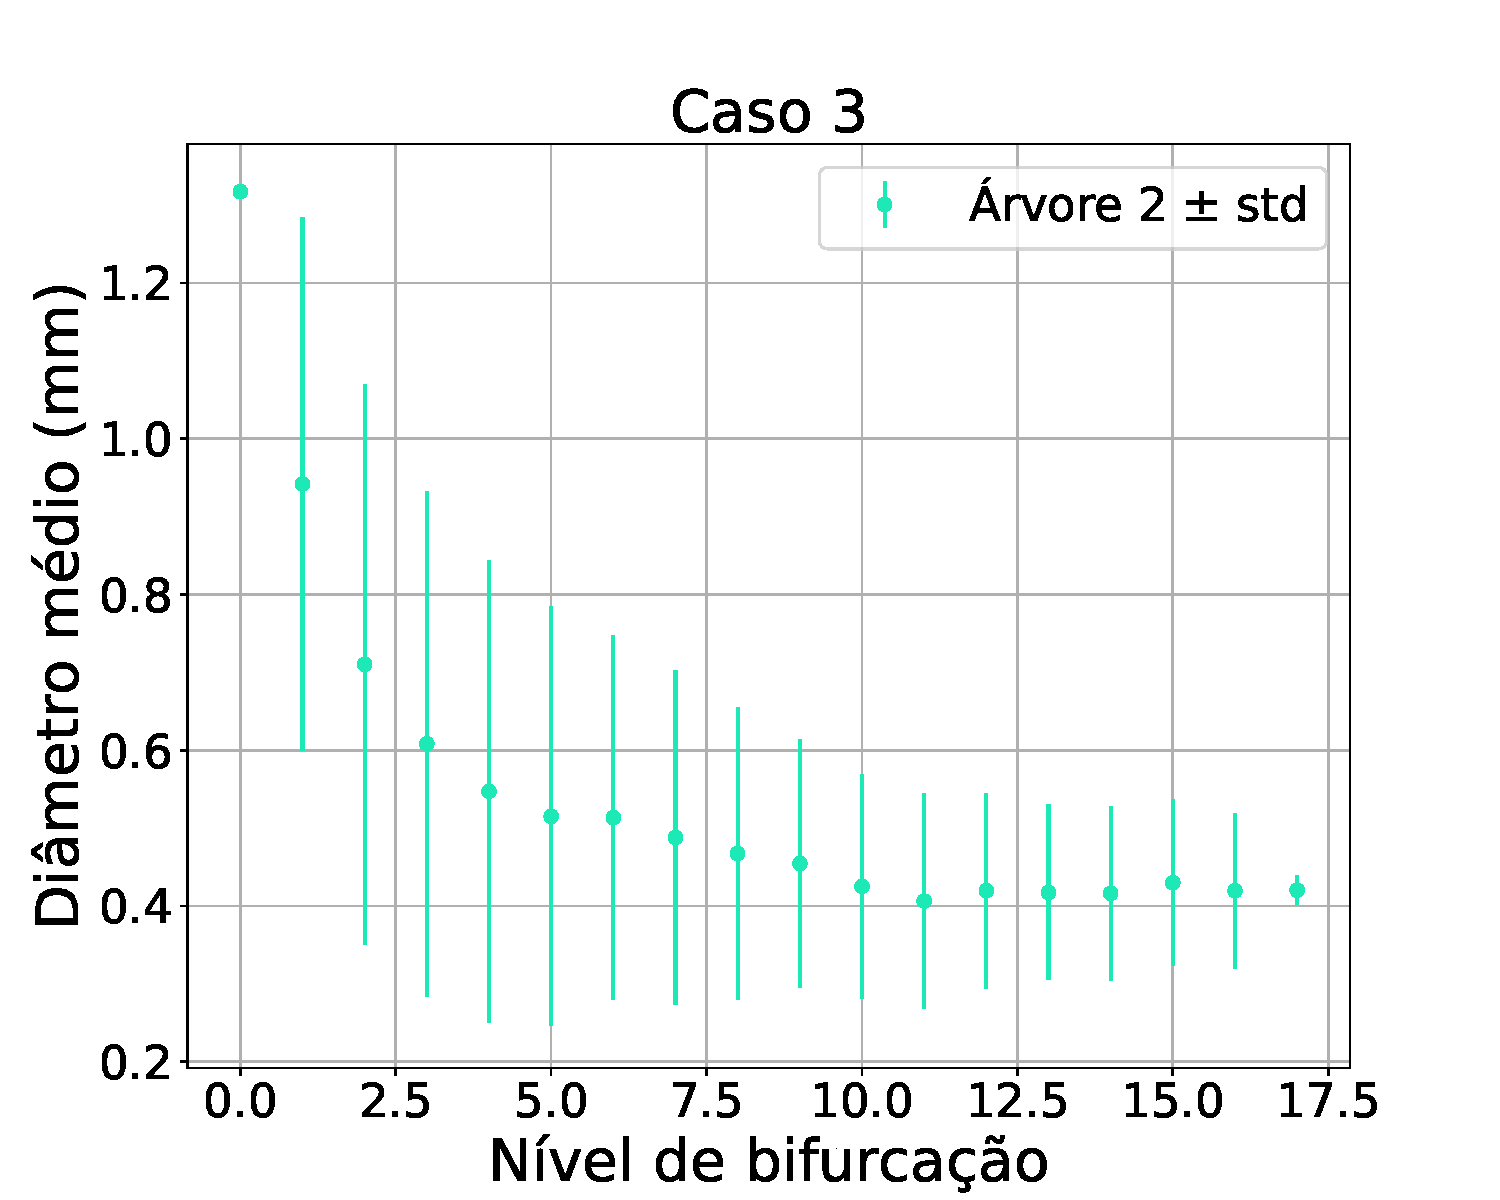
\includegraphics[scale=0.3]{figuras/floresta-com-coeficiente-de-invasao/2D/disco/duas-arvores-diametro-medio-750-250-tree-2.pdf}}

  \fonteAutor{2022}
  \label{fig:diametro-medio-floresta-com-invasao-caso-2d-parte1}
\end{figure}

\begin{figure}[!htb]
  \centering
  \captiondelim{: }
  \caption{Diâmetro médio do segmento em função de seu nível de bifurcação. 
  Florestas com duas árvores arteriais construídas com diferentes fluxos alvo: 
  (a), (b) Caso 4 (80\%--20\%); (c), (d) Caso 5 (83,33\%--16,67\%);  (e), (f) Caso 6 (85,71\%--14,29\%).}
  
  \subfloat[]{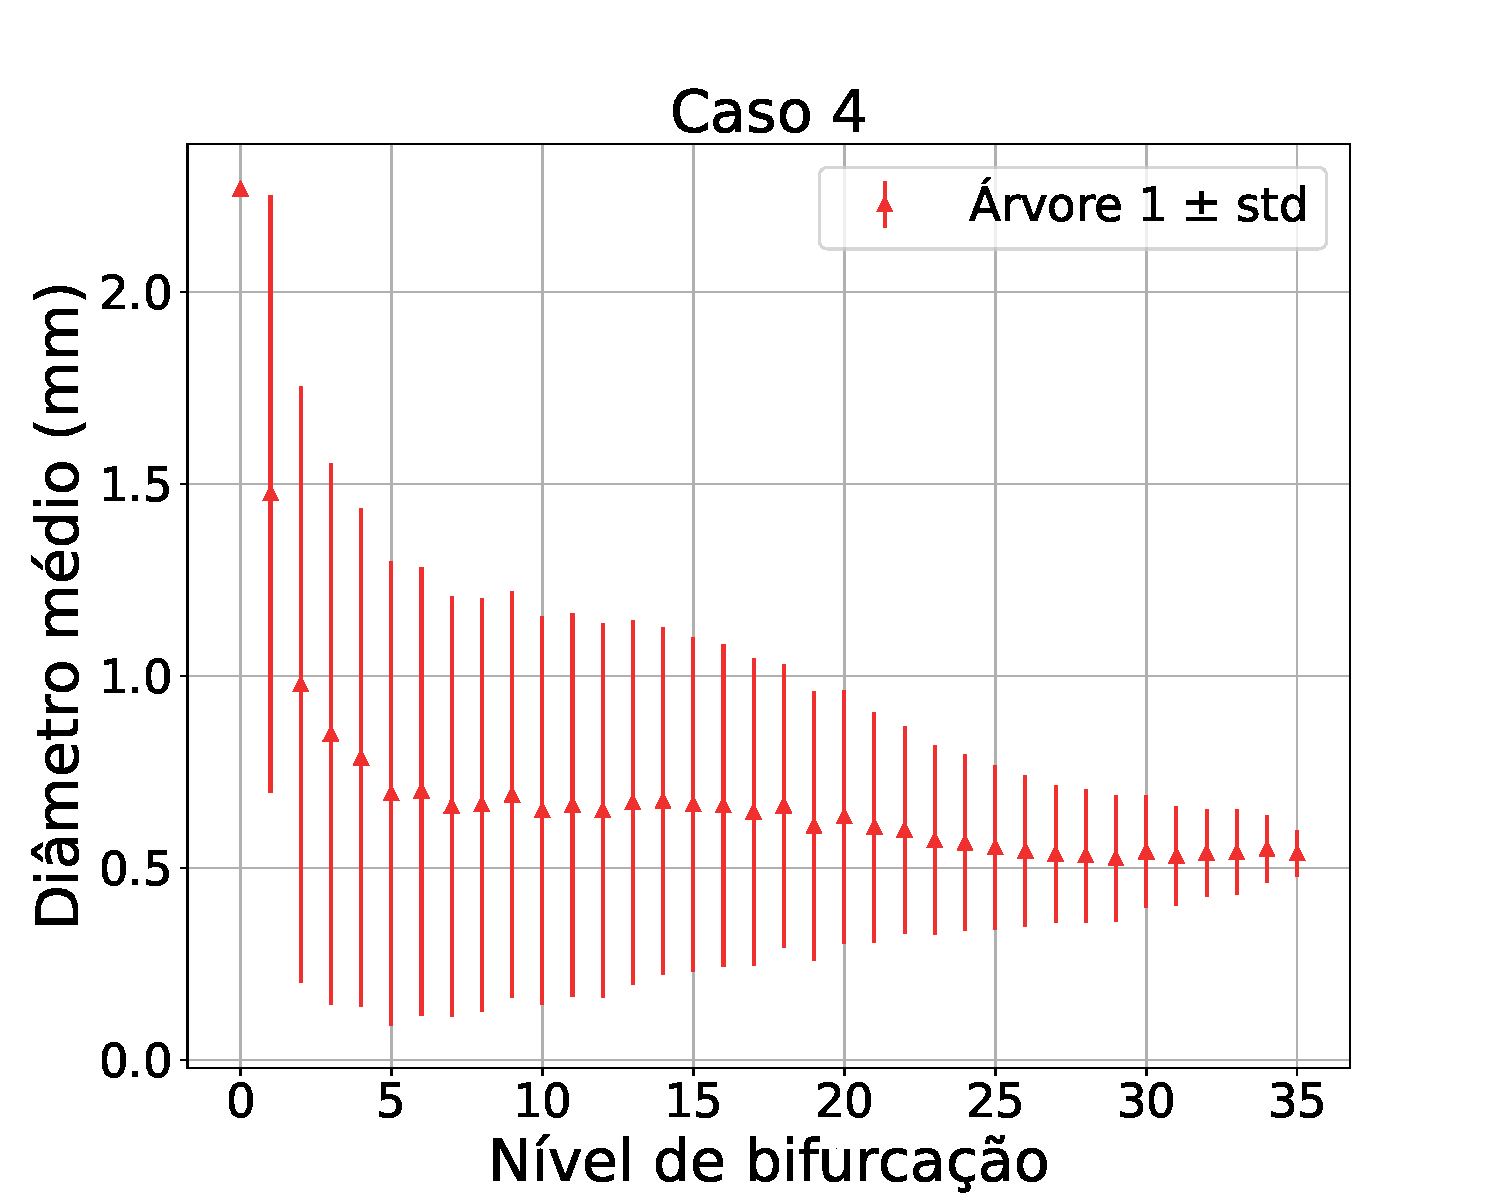
\includegraphics[scale=0.3]{figuras/floresta-com-coeficiente-de-invasao/2D/disco/duas-arvores-diametro-medio-800-200-tree-1.pdf}}
  \hspace{12pt}
  \subfloat[]{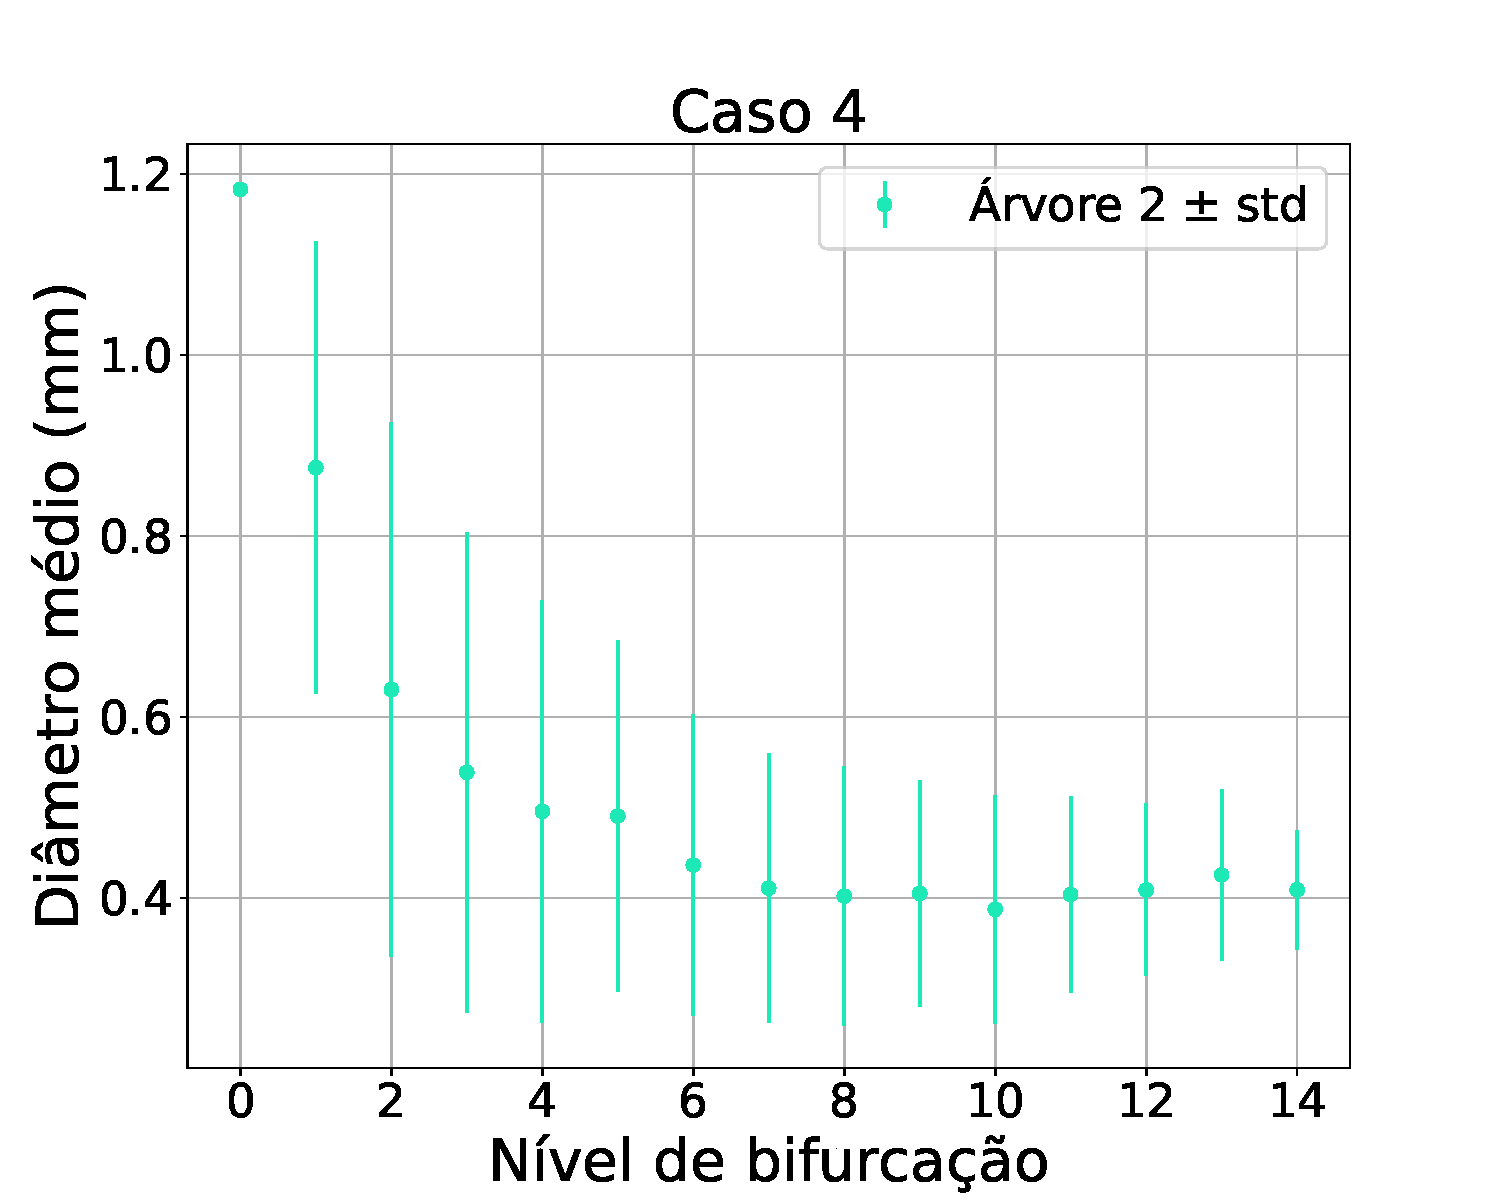
\includegraphics[scale=0.3]{figuras/floresta-com-coeficiente-de-invasao/2D/disco/duas-arvores-diametro-medio-800-200-tree-2.pdf}}

  \subfloat[]{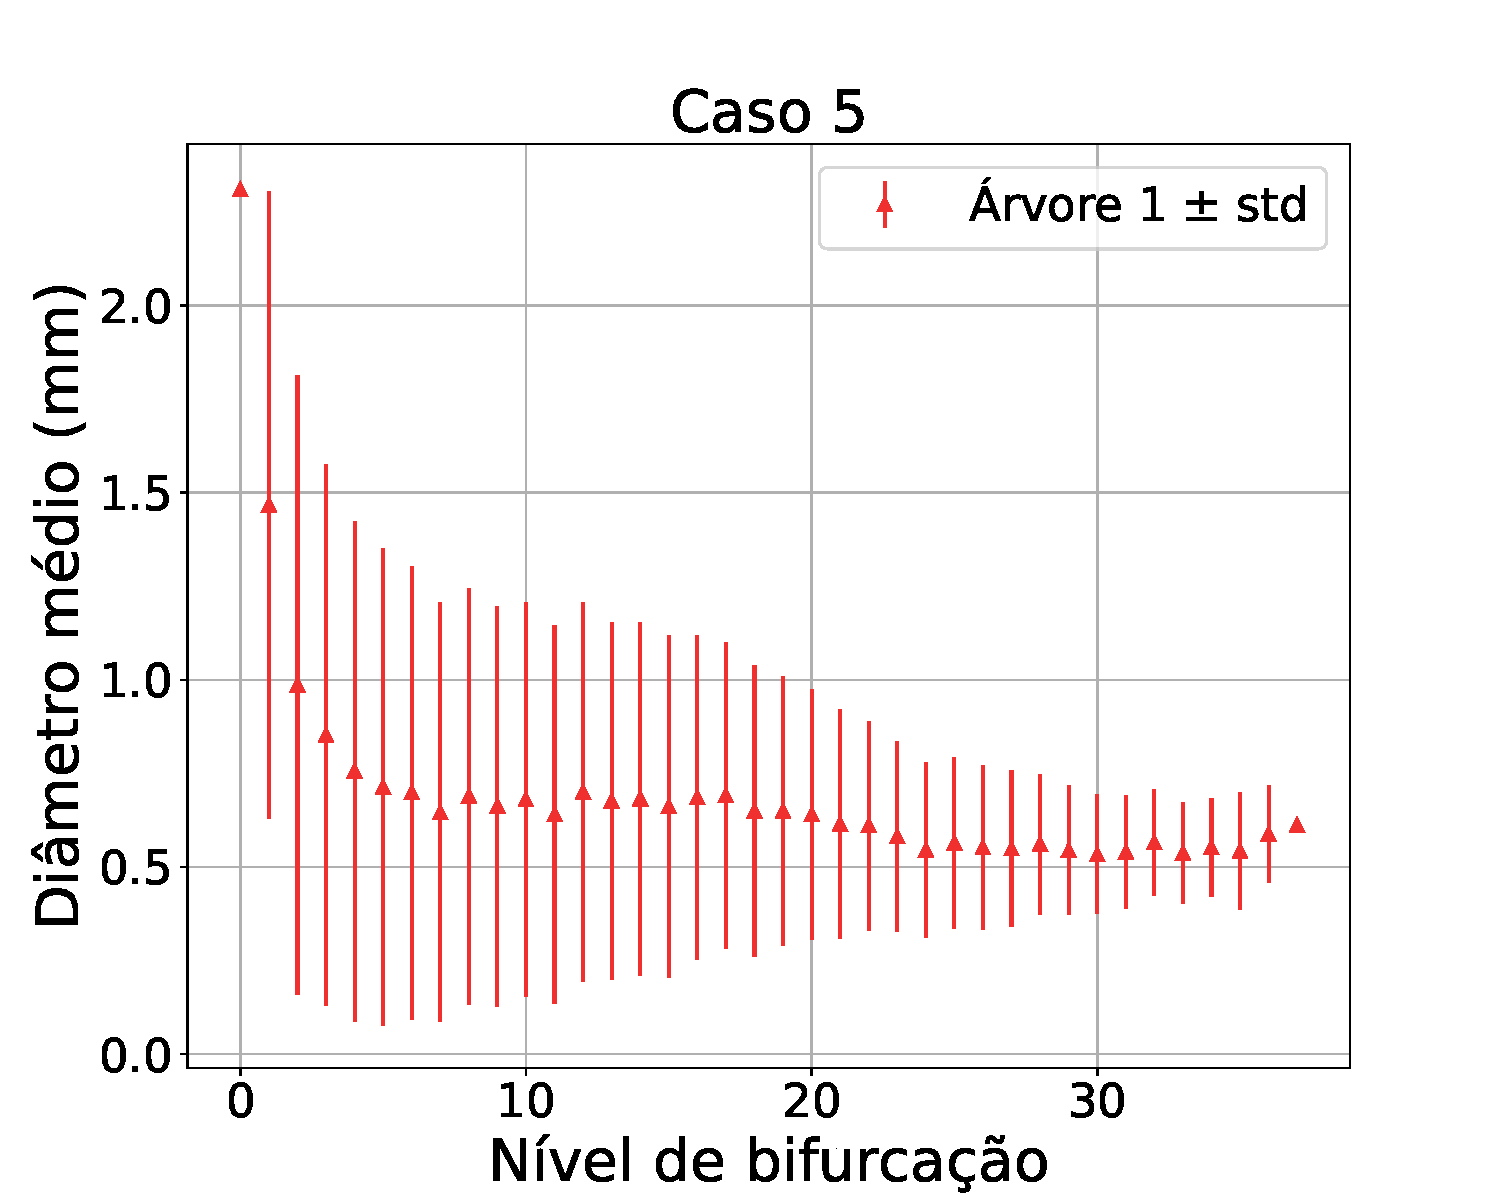
\includegraphics[scale=0.3]{figuras/floresta-com-coeficiente-de-invasao/2D/disco/duas-arvores-diametro-medio-834-166-tree-1.pdf}}
  \hspace{12pt}
  \subfloat[]{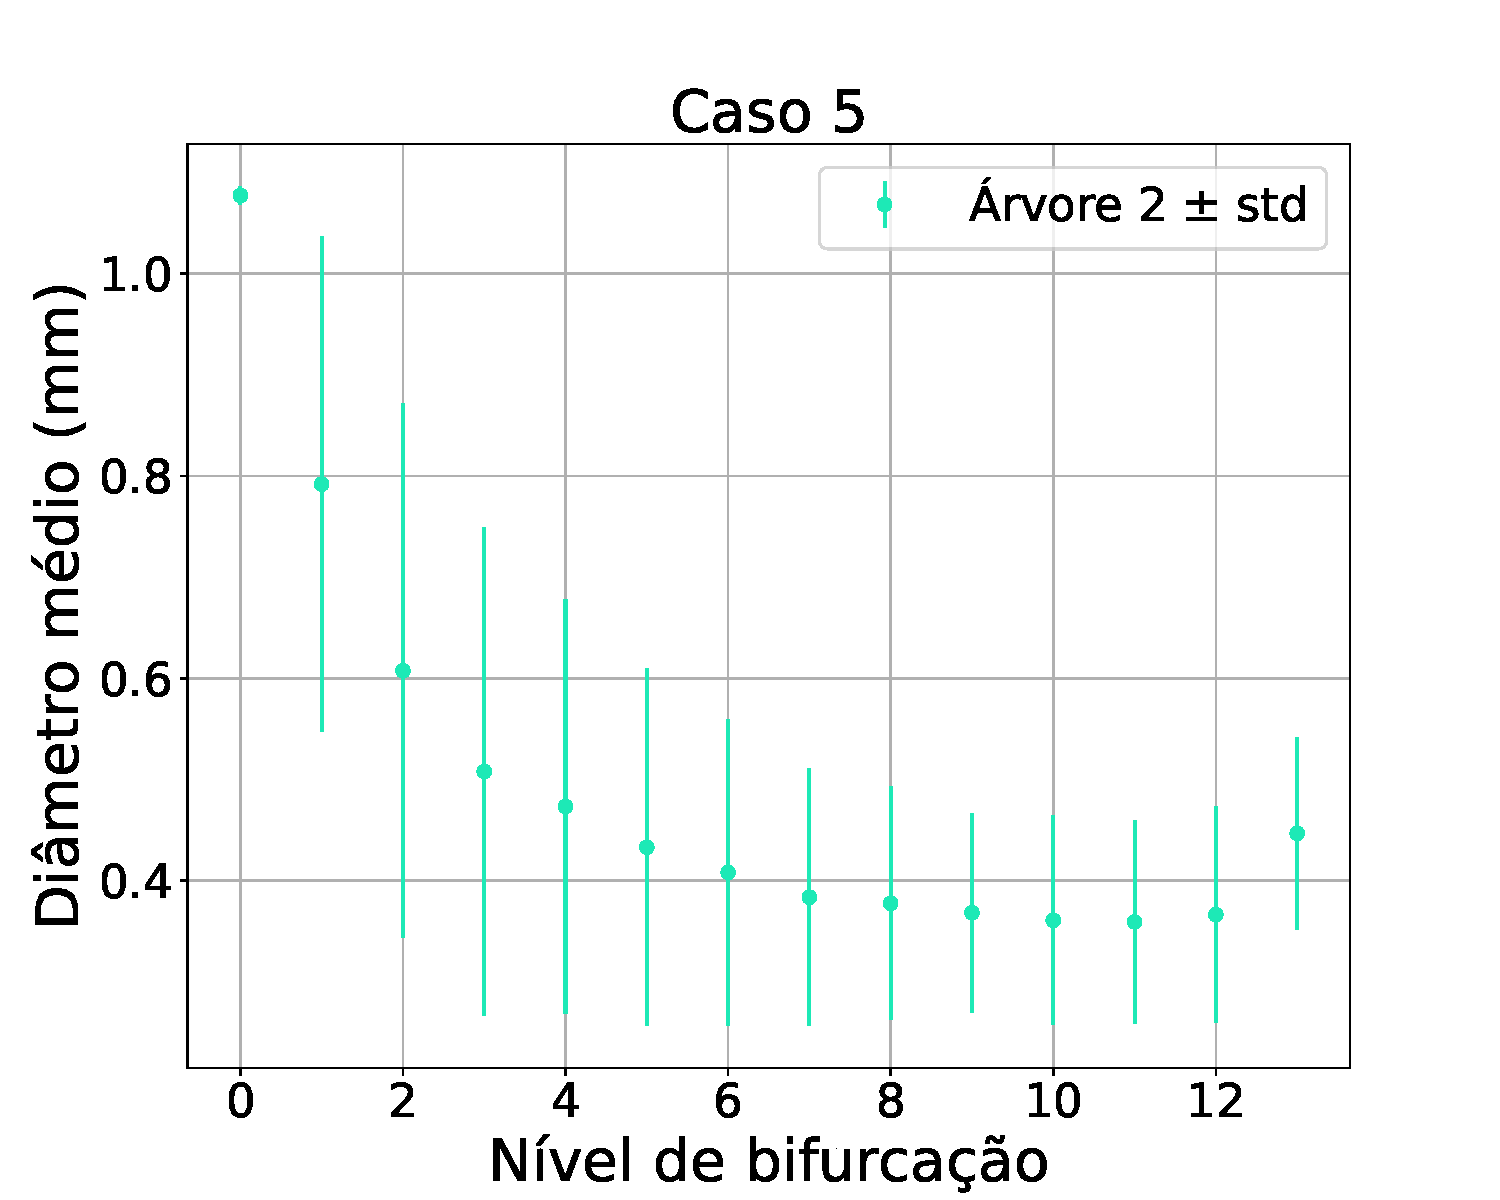
\includegraphics[scale=0.3]{figuras/floresta-com-coeficiente-de-invasao/2D/disco/duas-arvores-diametro-medio-834-166-tree-2.pdf}} 

  \subfloat[]{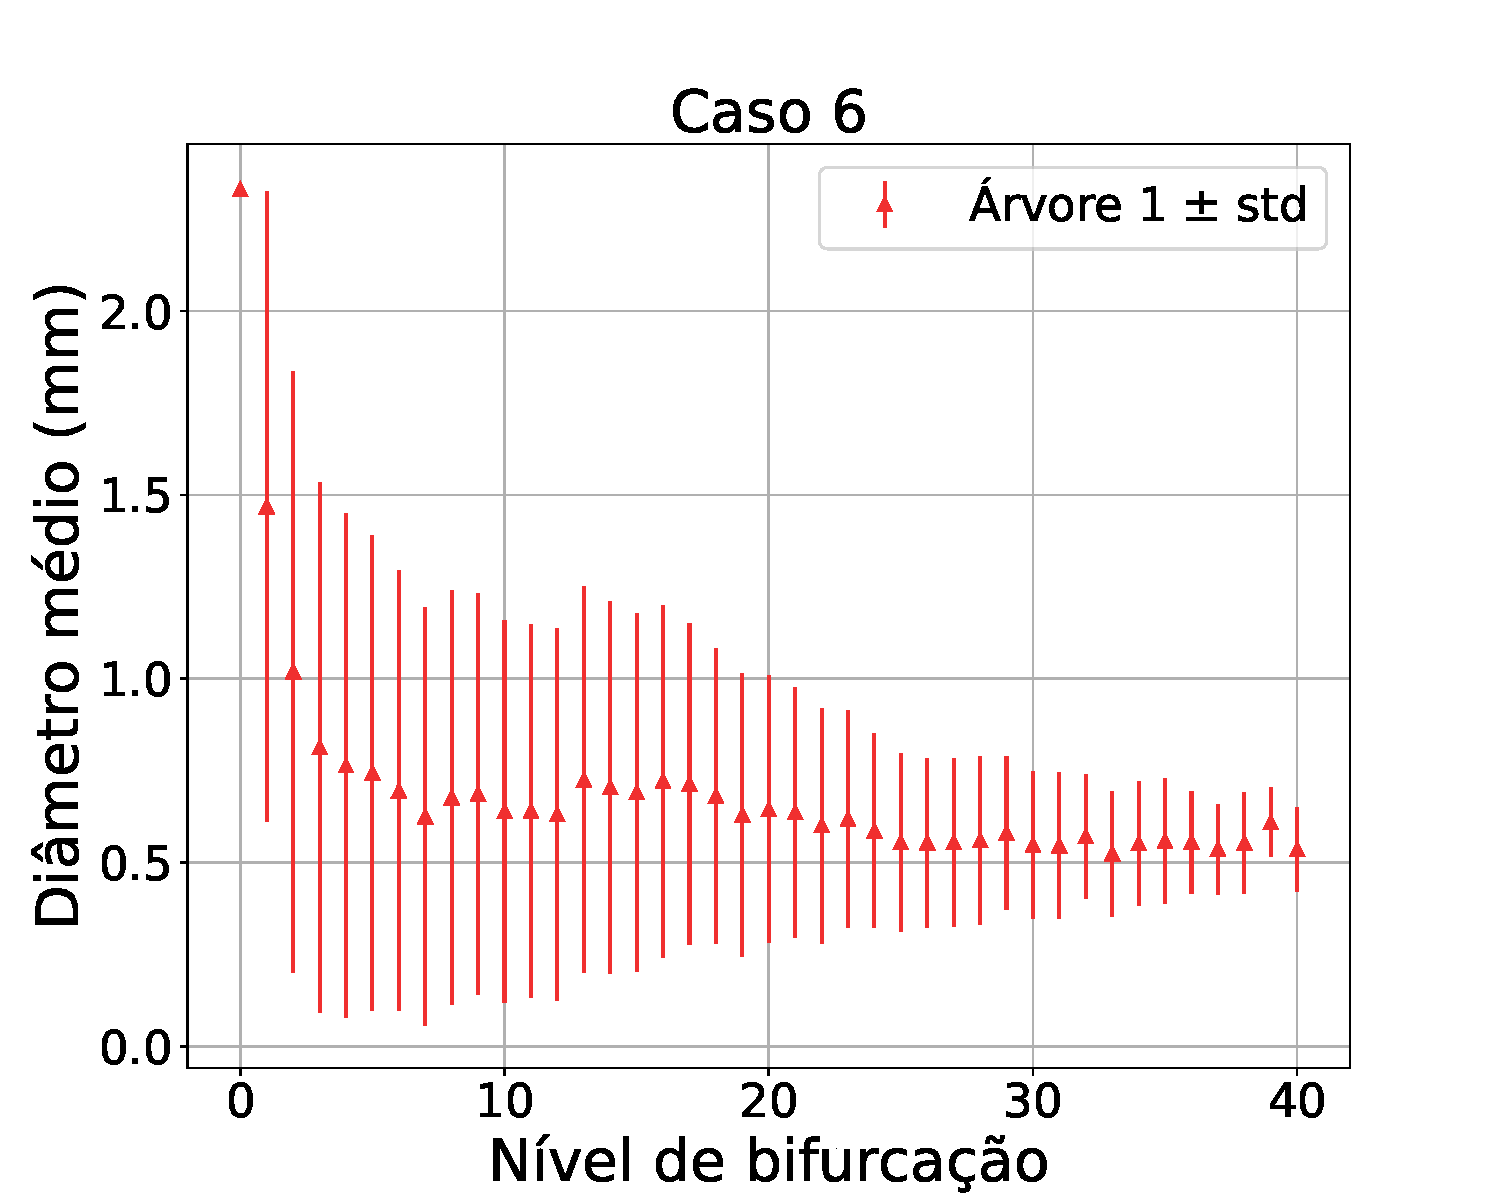
\includegraphics[scale=0.3]{figuras/floresta-com-coeficiente-de-invasao/2D/disco/duas-arvores-diametro-medio-857-143-tree-1.pdf}}
  \hspace{12pt}
  \subfloat[]{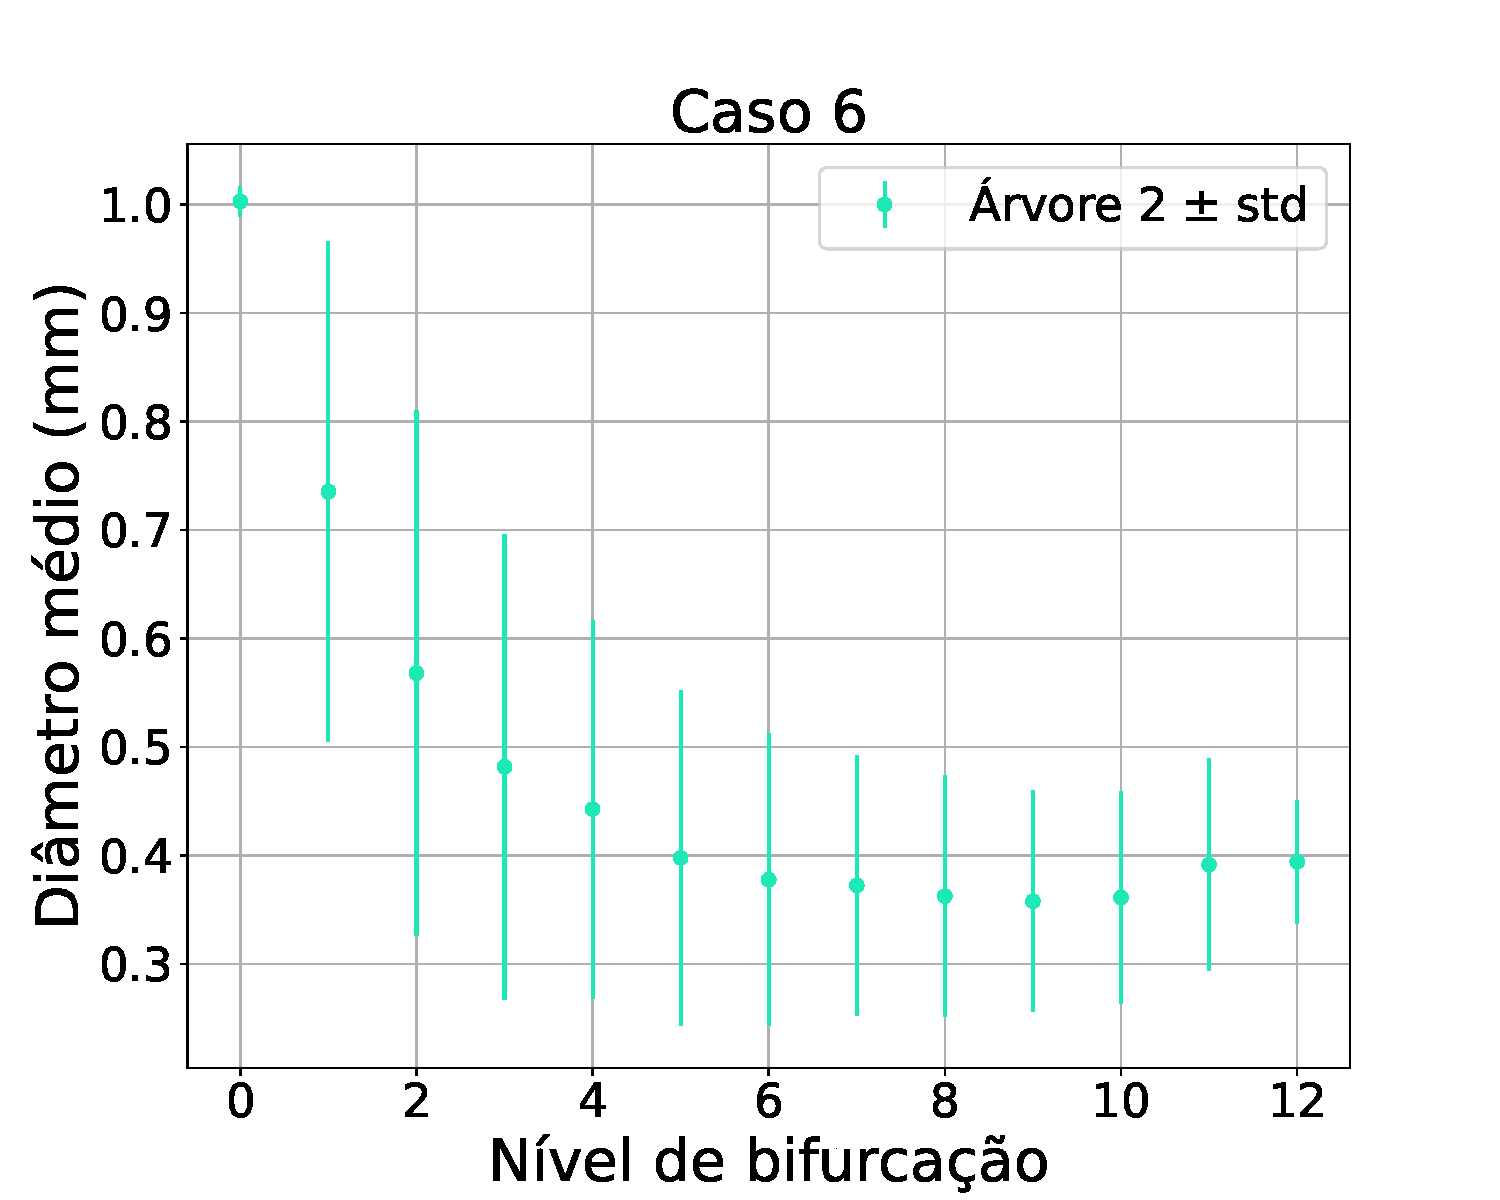
\includegraphics[scale=0.3]{figuras/floresta-com-coeficiente-de-invasao/2D/disco/duas-arvores-diametro-medio-857-143-tree-2.pdf}}

  \fonteAutor{2022}
  \label{fig:diametro-medio-floresta-com-invasao-caso-2d-parte2}
\end{figure}

\clearpage

\begin{figure}[!htb]
  \centering
  \captiondelim{: }
  \caption{Diâmetro médio do segmento em função de seu nível de bifurcação. 
  Florestas com duas árvores arteriais construídas com diferentes fluxos alvo: 
  (a), (b) Caso 7 (87,5\%--12,50\%); (c), (d) Caso 8 (88,89\%--11,11\%);  (e), (f) Caso 9 (90,00\%--10,00\%).}
  
  \subfloat[]{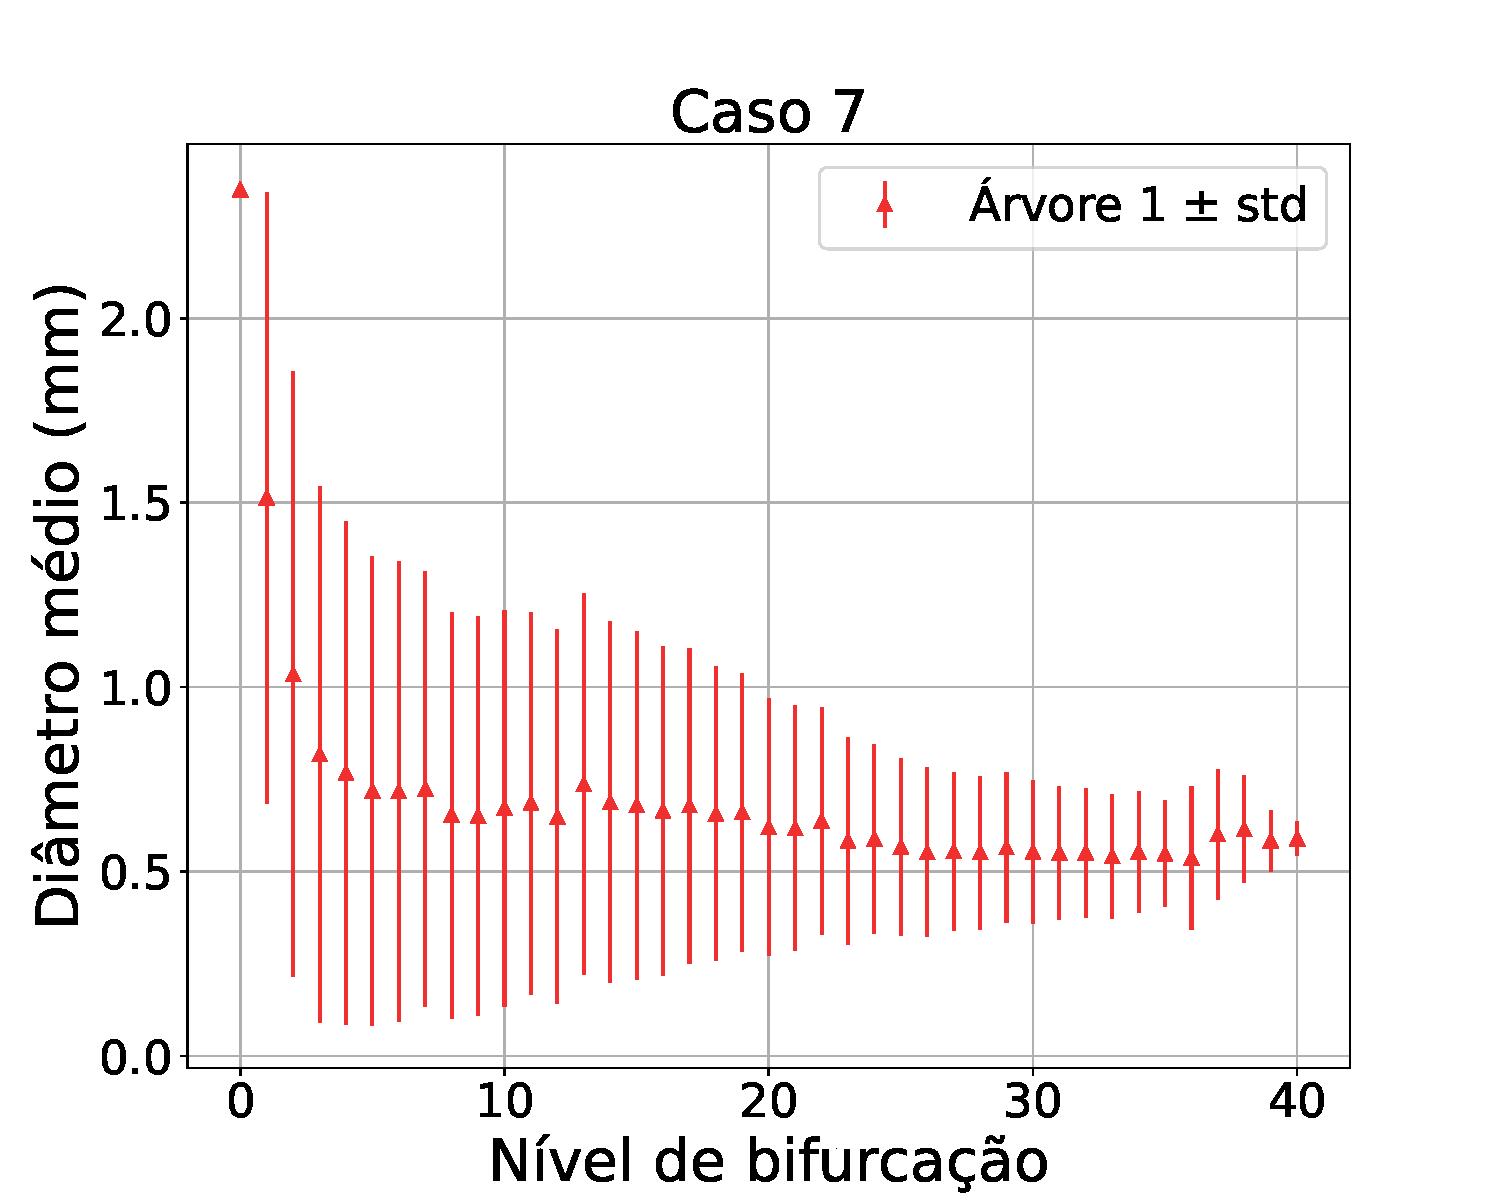
\includegraphics[scale=0.3]{figuras/floresta-com-coeficiente-de-invasao/2D/disco/duas-arvores-diametro-medio-875-125-tree-1.pdf}}
  \hspace{12pt}
  \subfloat[]{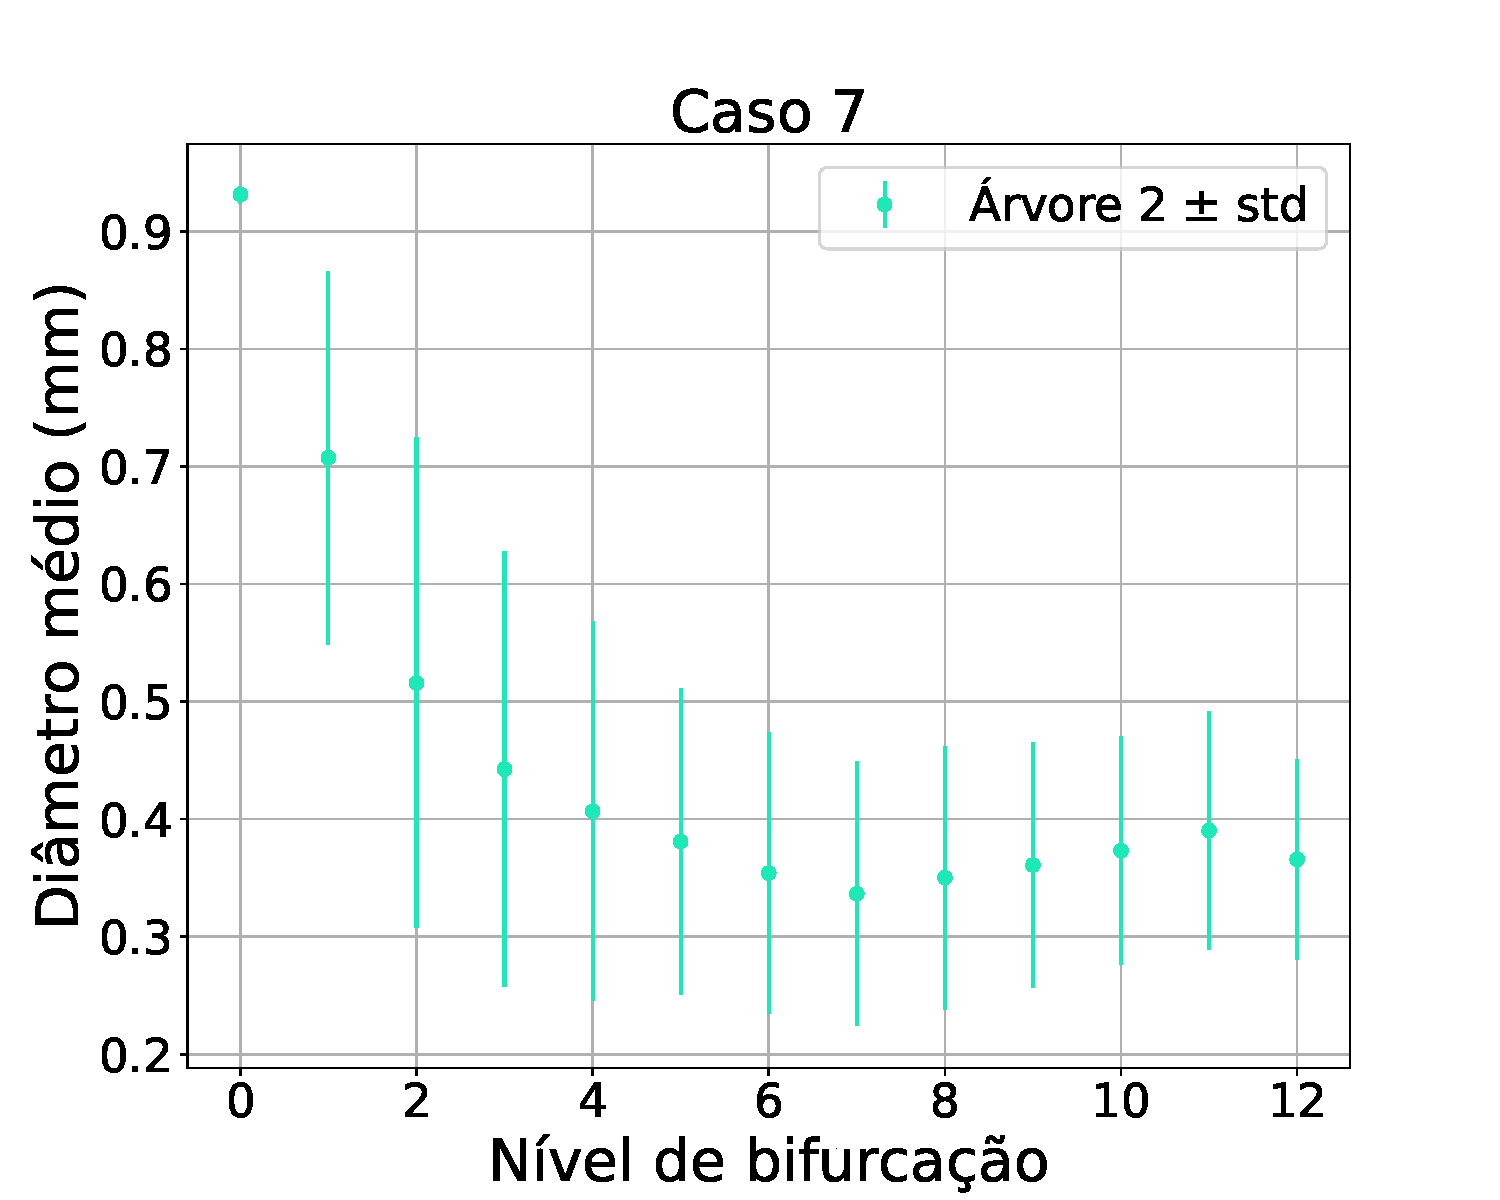
\includegraphics[scale=0.3]{figuras/floresta-com-coeficiente-de-invasao/2D/disco/duas-arvores-diametro-medio-875-125-tree-2.pdf}}

  \subfloat[]{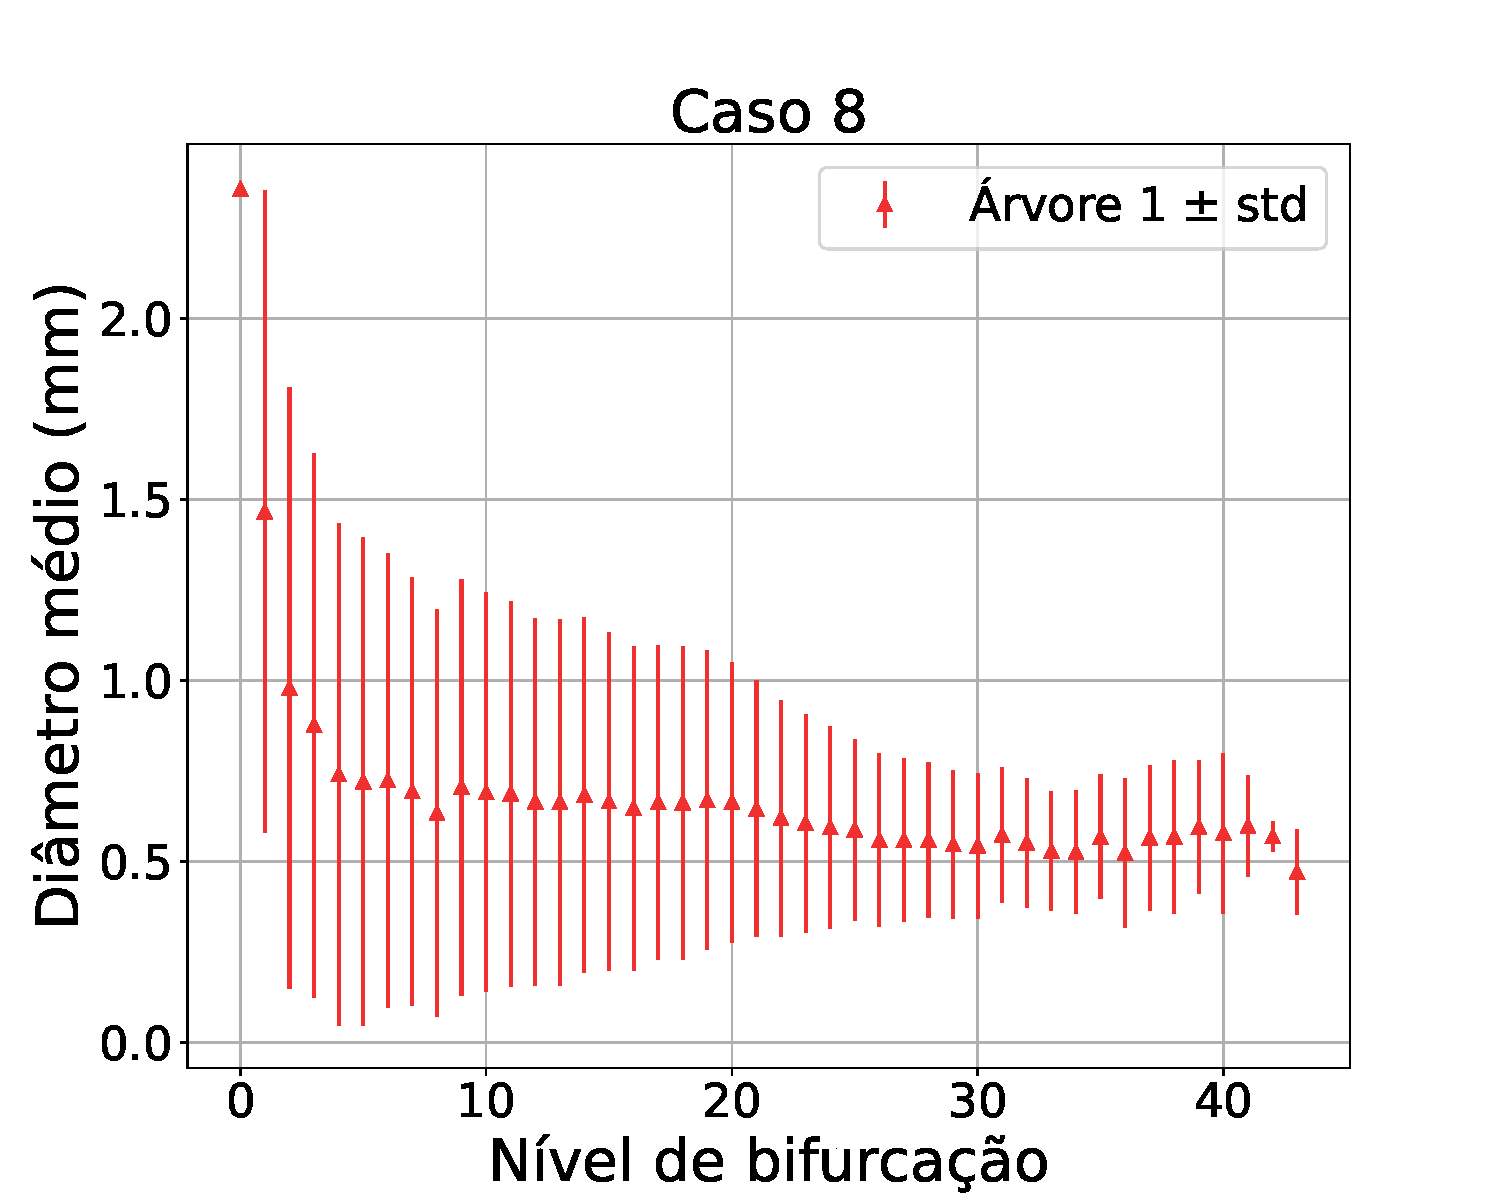
\includegraphics[scale=0.3]{figuras/floresta-com-coeficiente-de-invasao/2D/disco/duas-arvores-diametro-medio-889-111-tree-1.pdf}}
  \hspace{12pt}
  \subfloat[]{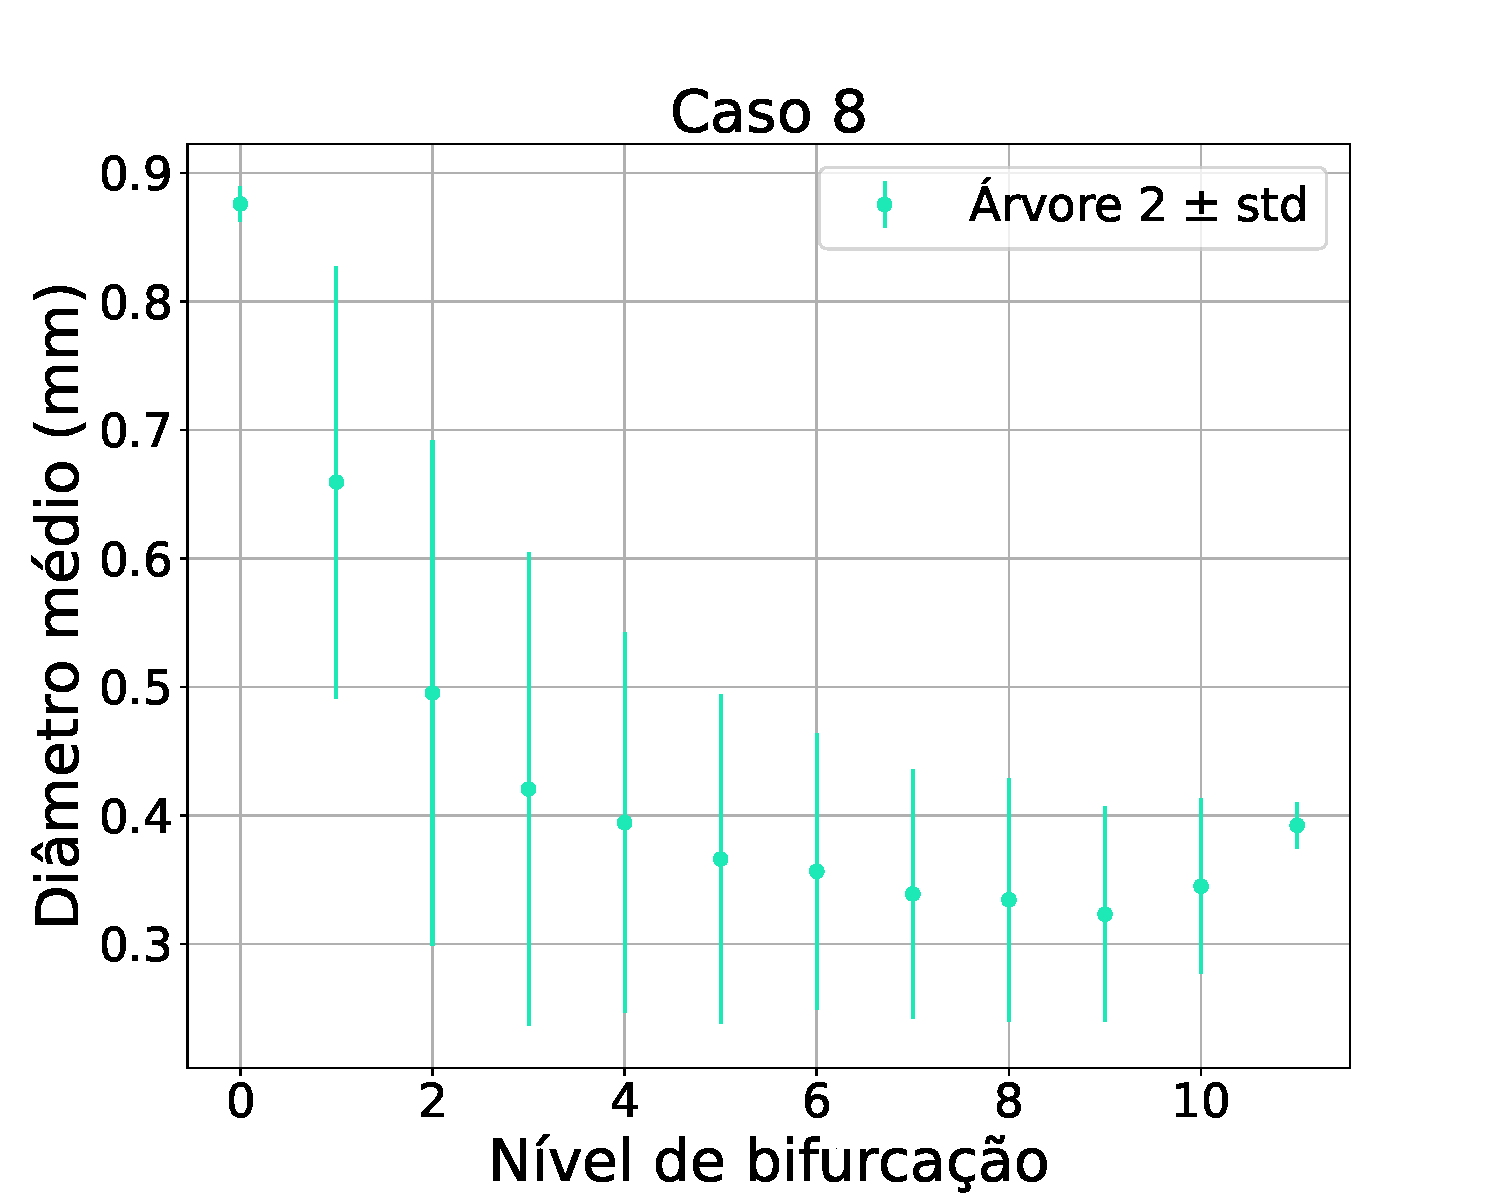
\includegraphics[scale=0.3]{figuras/floresta-com-coeficiente-de-invasao/2D/disco/duas-arvores-diametro-medio-889-111-tree-2.pdf}} 

  \subfloat[]{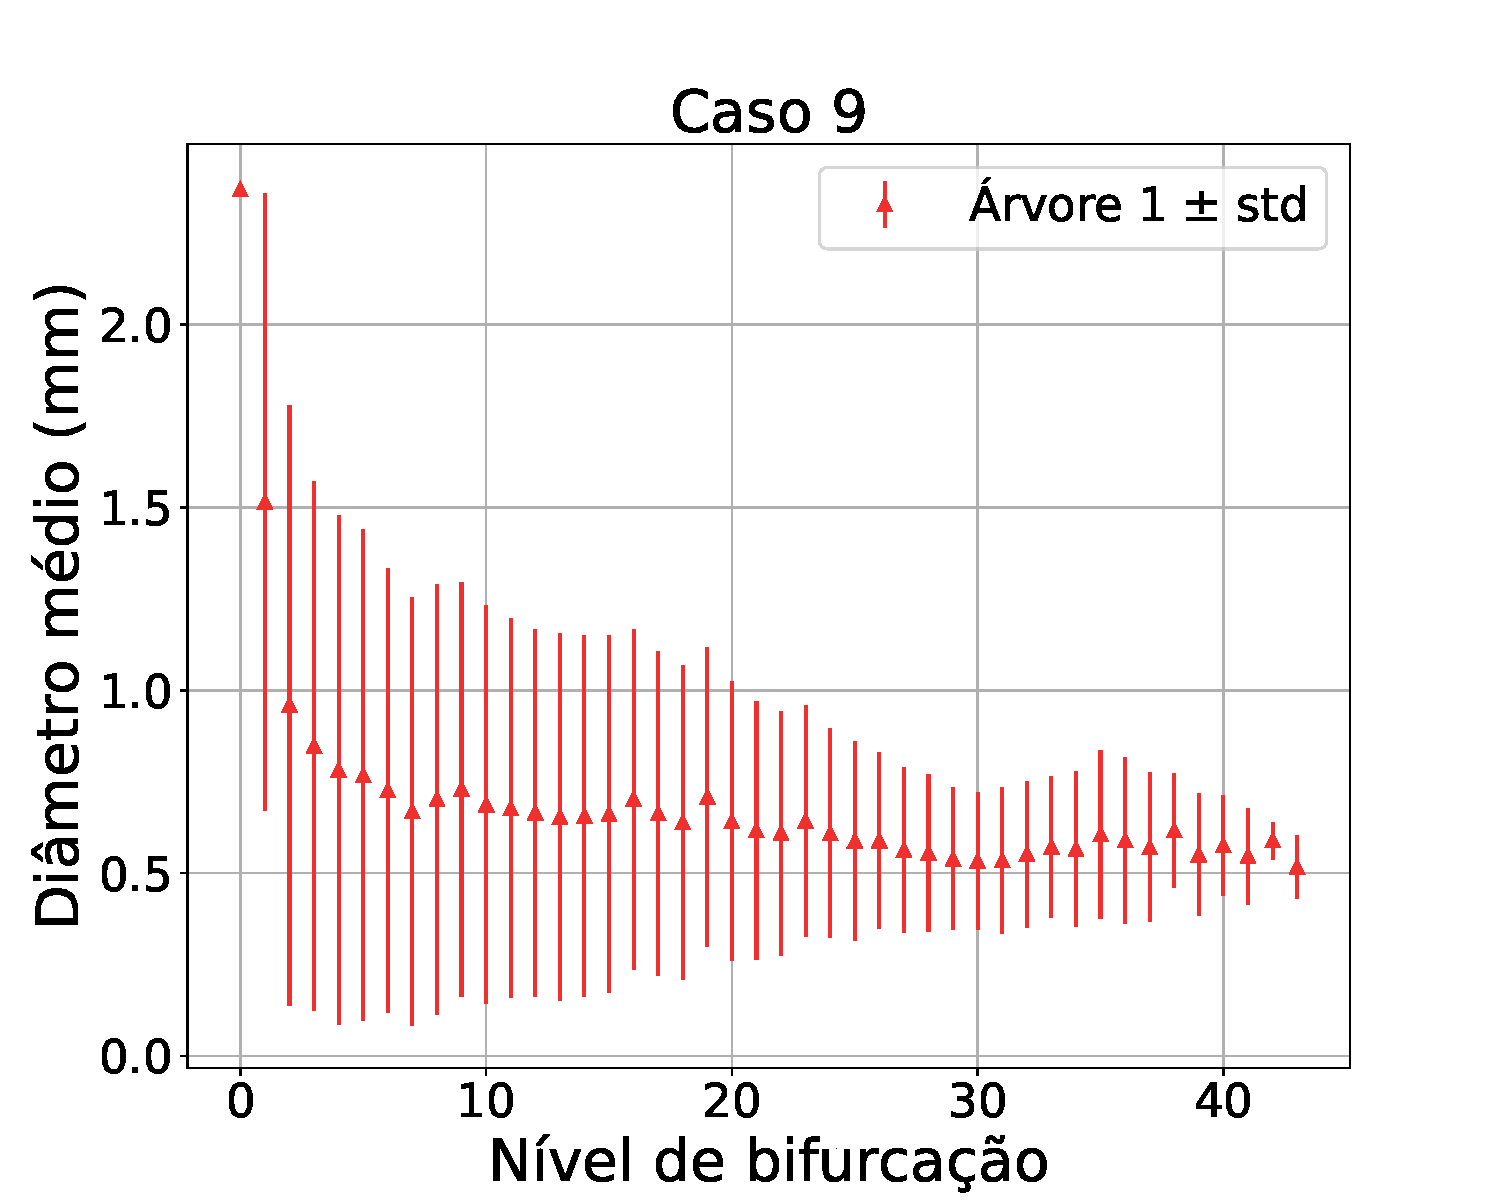
\includegraphics[scale=0.3]{figuras/floresta-com-coeficiente-de-invasao/2D/disco/duas-arvores-diametro-medio-900-100-tree-1.pdf}}
  \hspace{12pt}
  \subfloat[]{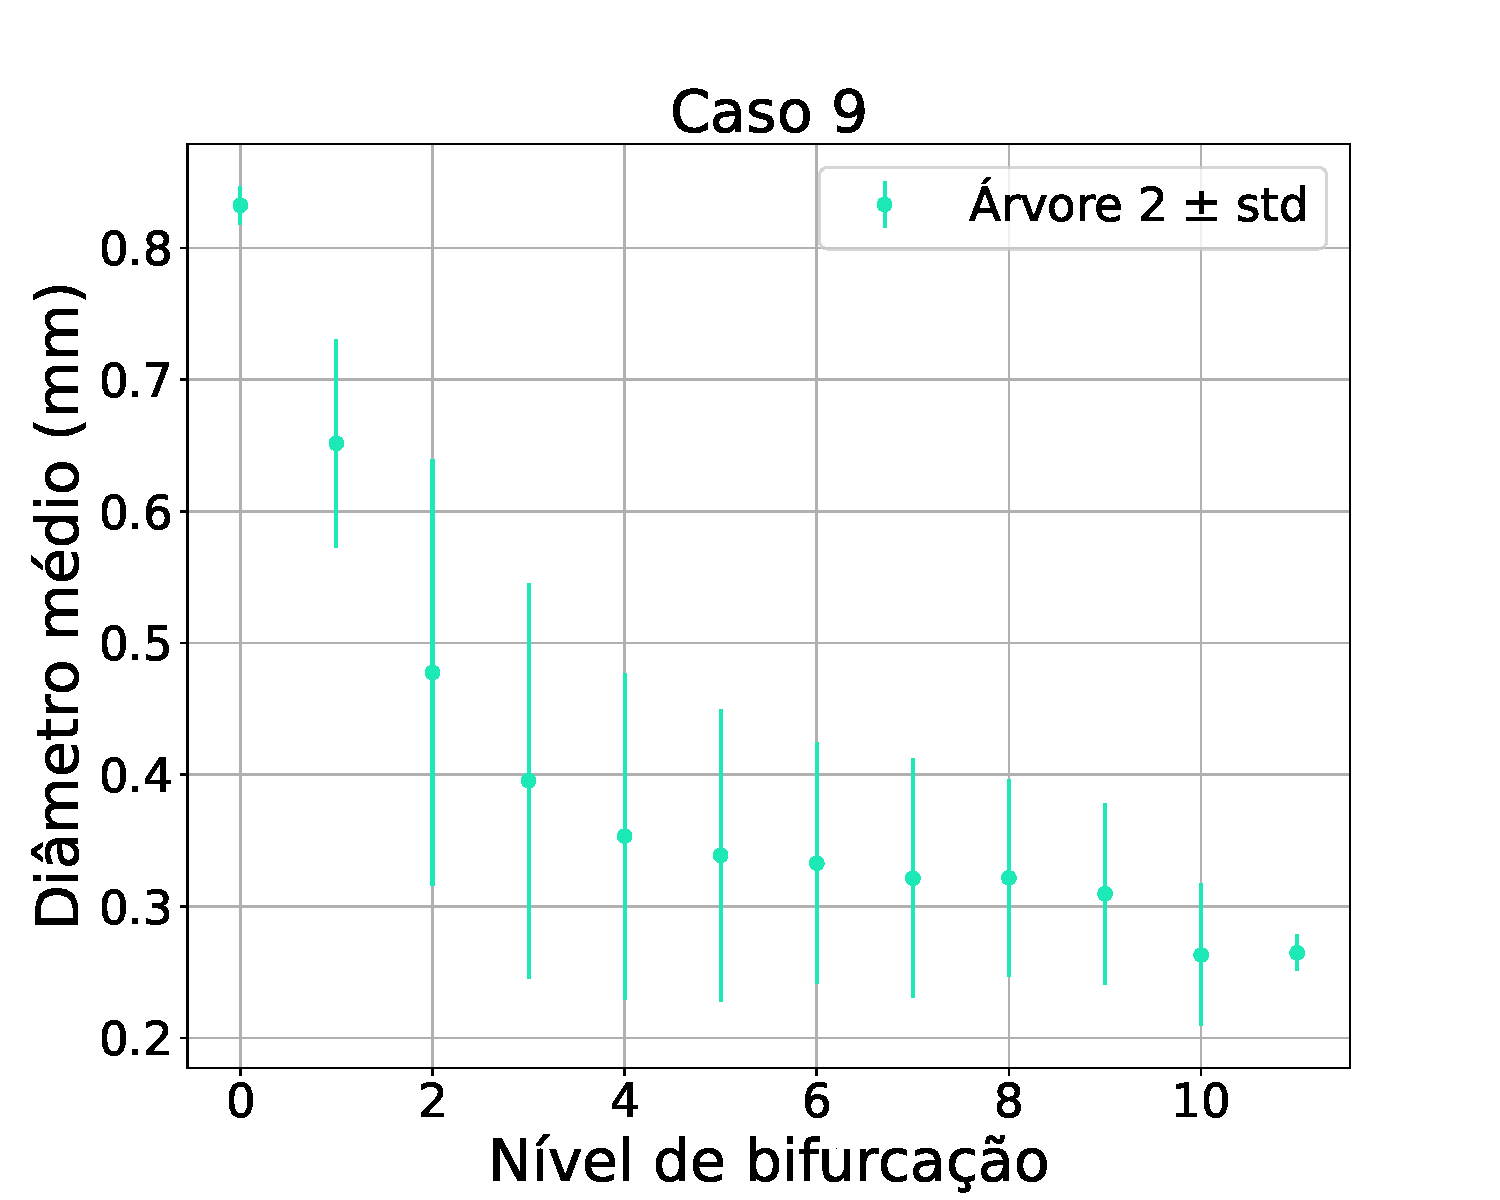
\includegraphics[scale=0.3]{figuras/floresta-com-coeficiente-de-invasao/2D/disco/duas-arvores-diametro-medio-900-100-tree-2.pdf}}

  \fonteAutor{2022}
  \label{fig:diametro-medio-floresta-com-invasao-caso-2d-parte3}
\end{figure}

\begin{figure}[!htb]
  \centering
  \captiondelim{: }
  \caption{Diâmetro médio do segmento em função de seu nível de bifurcação. 
  Florestas com duas árvores arteriais construídas com diferentes fluxos alvo: 
  (a), (b) Caso 10 (90,91\%--9,09\%).}
  
  \subfloat[]{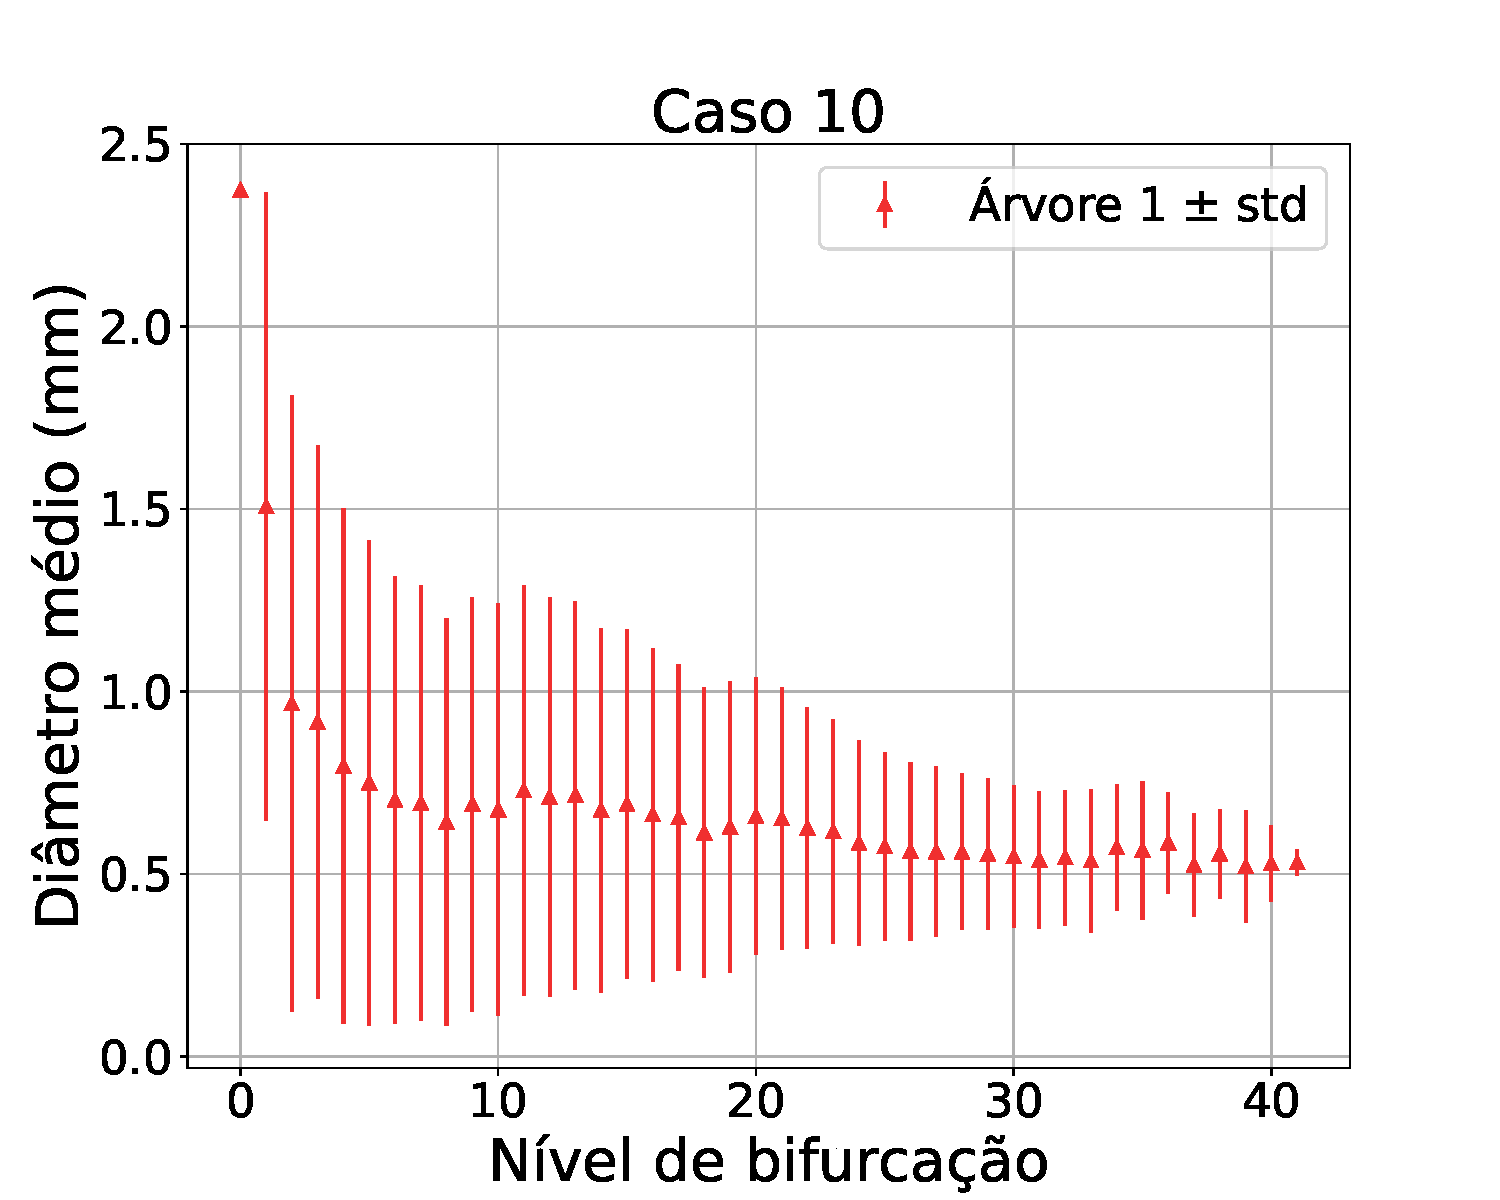
\includegraphics[scale=0.3]{figuras/floresta-com-coeficiente-de-invasao/2D/disco/duas-arvores-diametro-medio-909-91-tree-1.pdf}}
  \hspace{12pt}
  \subfloat[]{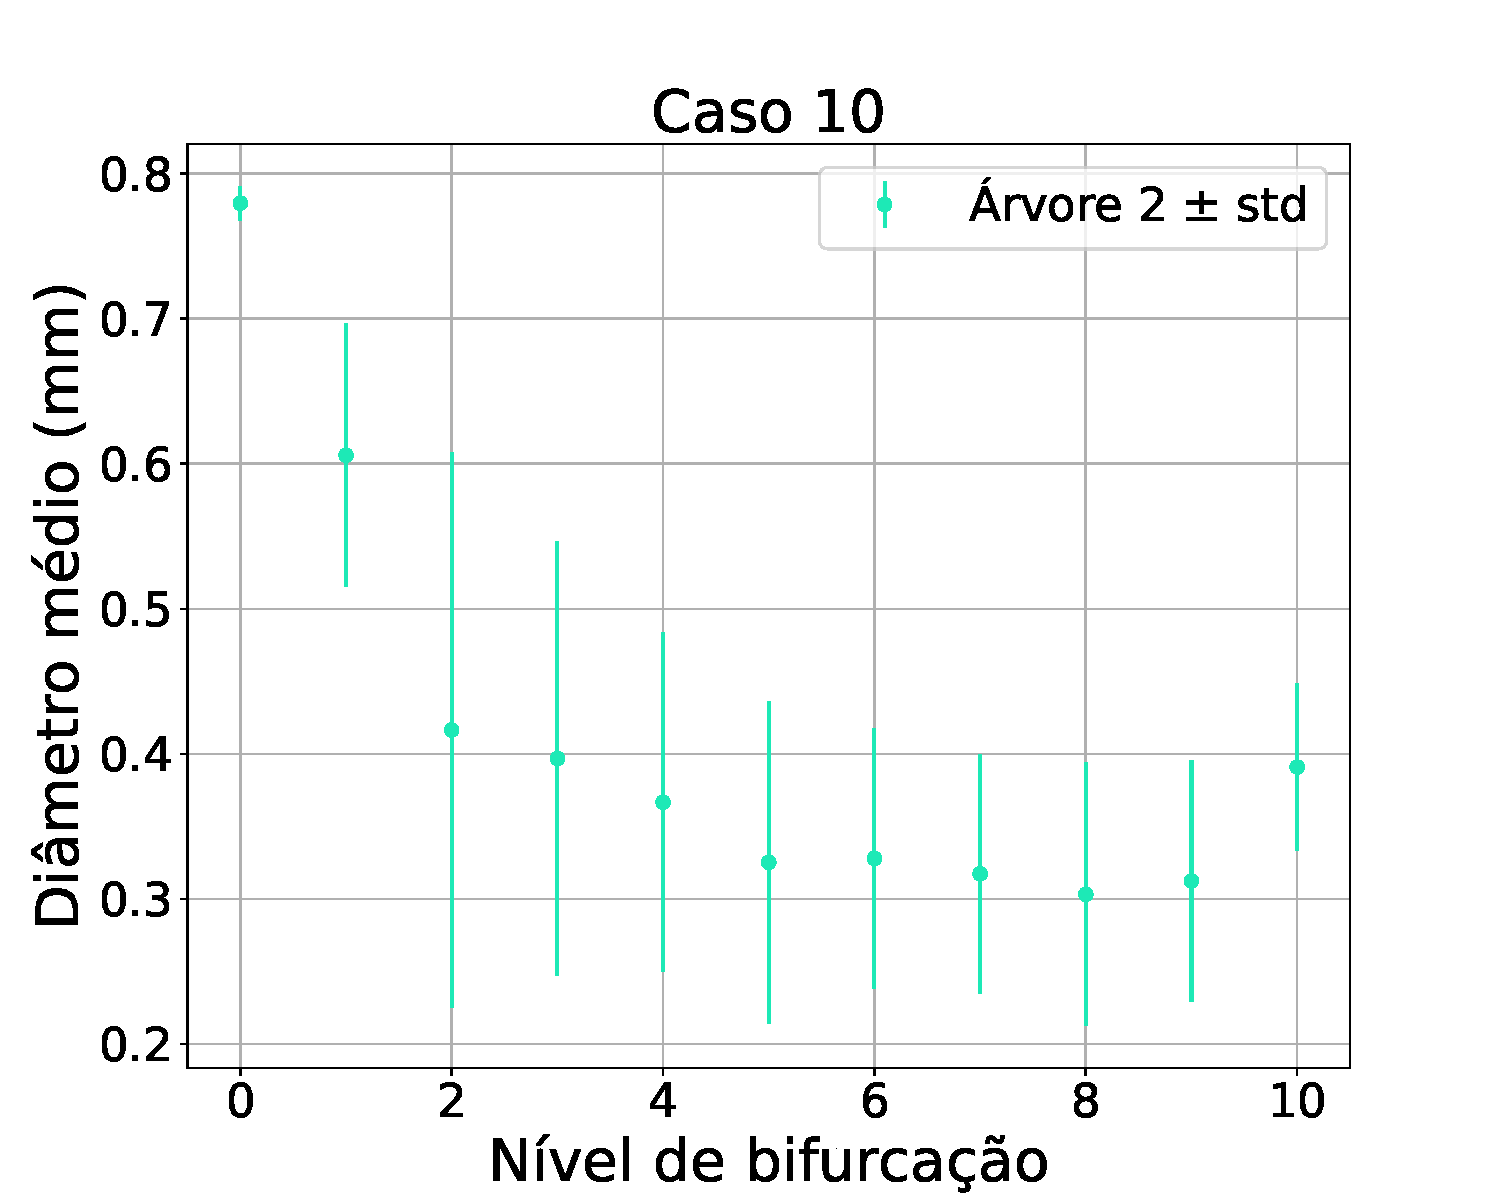
\includegraphics[scale=0.3]{figuras/floresta-com-coeficiente-de-invasao/2D/disco/duas-arvores-diametro-medio-909-91-tree-2.pdf}}

  \fonteAutor{2022}
  \label{fig:diametro-medio-floresta-com-invasao-caso-2d-parte4}
\end{figure}

Para ilustrar a influência do coeficiente de invasão $\alpha$, foram executadas dez simulações 
com uma mesma semente do gerador dSFMT, construindo florestas com duas árvores ($N_{trees} = 2$),
número total de terminais igual a 250 ($N_{term} = 250$) e fluxo alvo em dois casos:
(i) 50\%--50\%; (ii) 75\%--25\%.
As Figuras~\ref{fig:coeficiente-de-invasao-floresta-com-invasao-parte1} e~\ref{fig:coeficiente-de-invasao-floresta-com-invasao-parte2} 
ilustram as florestas criadas. Destaca-se que $\alpha$ pode ser ajustado conforme 
necessário em diferentes domínios de perfusão.

\clearpage

\begin{figure}[!htb]
  \centering
  \captiondelim{: }
  \caption{Florestas com duas árvores e fluxo alvo de 50\% cada árvore. A árvore 1 está em vermelho e a árvore 2 em verde. Coeficientes de invasão:
  (a) 0,0. (b) 0,25. (c) 0,5. (d) 0,75. (e) 1,0.}
  
  \subfloat[]{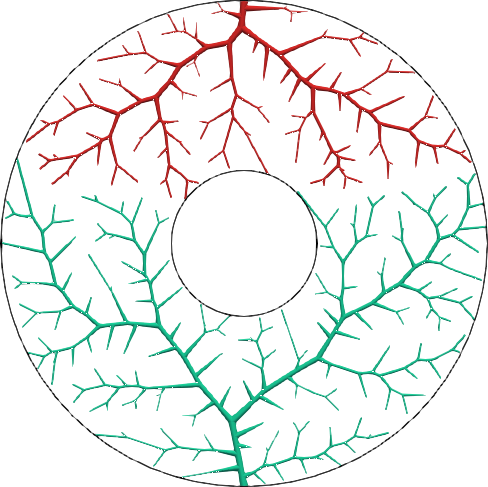
\includegraphics[scale=0.35]{figuras/floresta-com-coeficiente-de-invasao/2D/disco/floresta-coeficiente-de-invasao-0.0-500-500.png}}
  \hspace{12pt}
  \subfloat[]{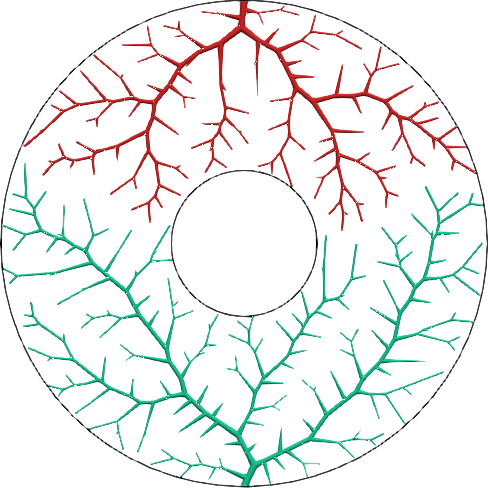
\includegraphics[scale=0.35]{figuras/floresta-com-coeficiente-de-invasao/2D/disco/floresta-coeficiente-de-invasao-0.25-500-500.png}}

  \subfloat[]{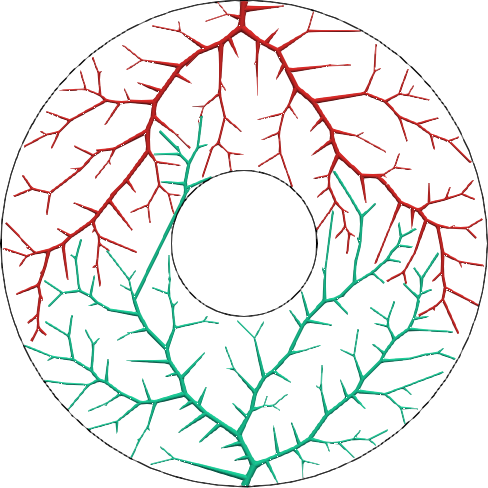
\includegraphics[scale=0.35]{figuras/floresta-com-coeficiente-de-invasao/2D/disco/floresta-coeficiente-de-invasao-0.5-500-500.png}}
  \hspace{12pt}
  \subfloat[]{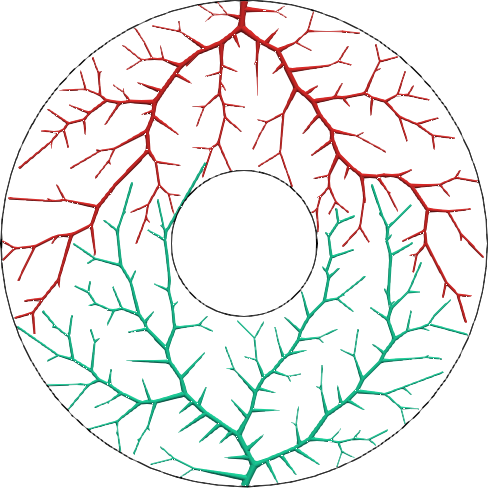
\includegraphics[scale=0.35]{figuras/floresta-com-coeficiente-de-invasao/2D/disco/floresta-coeficiente-de-invasao-0.75-500-500.png}}

  \subfloat[]{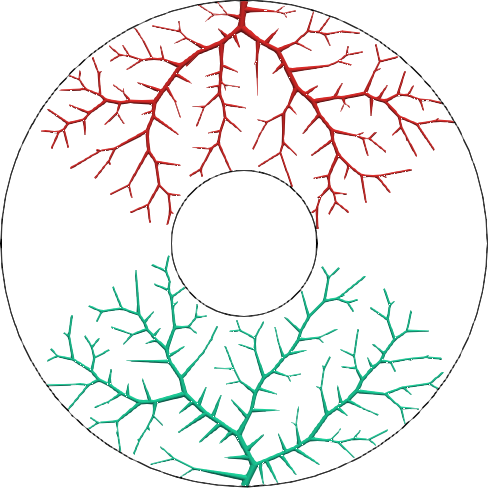
\includegraphics[scale=0.35]{figuras/floresta-com-coeficiente-de-invasao/2D/disco/floresta-coeficiente-de-invasao-1.0-500-500.png}}
  
  \fonteAutor{2022}
  \label{fig:coeficiente-de-invasao-floresta-com-invasao-parte1}
\end{figure}

\begin{figure}[!htb]
  \centering
  \captiondelim{: }
  \caption{Florestas com duas árvores e fluxo alvo de 75\% (árvore 1 em vermelho) e 25\% (árvore 2 em verde). Coeficientes de invasão:
  (a) 0,0. (b) 0,25. (c) 0,5. (d) 0,75. (e) 1,0.}

  \subfloat[]{\includegraphics[scale=0.35]{figuras/floresta-com-coeficiente-de-invasao/2D/disco/floresta-coeficiente-de-invasao-0.0-750-250.png}}
  \hspace{12pt}
  \subfloat[]{\includegraphics[scale=0.35]{figuras/floresta-com-coeficiente-de-invasao/2D/disco/floresta-coeficiente-de-invasao-0.25-750-250.png}}

  \subfloat[]{\includegraphics[scale=0.35]{figuras/floresta-com-coeficiente-de-invasao/2D/disco/floresta-coeficiente-de-invasao-0.5-750-250.png}}
  \hspace{12pt}
  \subfloat[]{\includegraphics[scale=0.35]{figuras/floresta-com-coeficiente-de-invasao/2D/disco/floresta-coeficiente-de-invasao-0.75-750-250.png}}

  \subfloat[]{\includegraphics[scale=0.35]{figuras/floresta-com-coeficiente-de-invasao/2D/disco/floresta-coeficiente-de-invasao-1.0-750-250.png}}

  \fonteAutor{2022}
  \label{fig:coeficiente-de-invasao-floresta-com-invasao-parte2}
\end{figure}

\subsection{Caso tridimensional com duas árvores}\label{sec:floresta-com-invasao-caso-3d}

A Tabela~\ref{tab:resultados-floresta-com-invasao-3d} resume os resultados
das simulações para verificar o fluxo obtido e o território ocupado, em contraste com o 
fluxo alvo fornecido.
Verifica-se que o erro relativo médio entre o fluxo obtido e o fluxo alvo foi 
de $0,023 \pm 0,038$. Isso representa um erro pouco maior que $2\%$. 
Além disso, a relação entre o fluxo obtido e o território ocupado estão correlacionados com um
coeficiente de $0,996$.

A Tabela~\ref{tab:resultados-lei-alometrica-floresta-com-invasao-3d} apresenta os resultados 
para estudar a lei alométrica~\eqref{eq:desenvolvimento-lei-alometrica}. Destaca-se que os valores
de $\delta_{1, 2}$ dessa lei ficaram próximos de $0,25$.

As Figuras~\ref{fig:ilustracoes-floresta-com-invasao-3d-parte1} e~\ref{fig:ilustracoes-floresta-com-invasao-3d-parte2} ilustram 
dez florestas obtidas considerando uma mesma semente do gerador dSFMT. Em cada floresta a cor vermelha foi utilizada 
para ilustrar a árvore 1 e a cor verde a árvore 2.
Já nas Figuras~\ref{fig:diametro-medio-floresta-com-invasao-caso-3d-parte1},\ 
~\ref{fig:diametro-medio-floresta-com-invasao-caso-3d-parte2},\ 
~\ref{fig:diametro-medio-floresta-com-invasao-caso-3d-parte3}\ 
e~\ref{fig:diametro-medio-floresta-com-invasao-caso-3d-parte4} são apresentadas 
as curvas morfométricas que relacionam o diâmetro médio 
do segmento em função de seu nível de bifurcação. Nota-se que essas curvas apresentam
o mesmo comportamento de decaimento conforme~\cite{Karch1999}.

\clearpage

\begin{table}[!htb]
  \centering
  \captiondelim{: }
  \caption{Resultados obtidos com a construção de florestas de árvores circulatórias 
empregando o Algoritmo~\ref{algo:FlorestaDeArvoresComInvasao}.}
\begin{tabular}{|c|c|c|c|c|}
\hline
Caso & Fluxo alvo (\%) & Fluxo obtido (\%) & Território (\%) & Volume (\%) \\ \hline
\multirow{2}{*}{1} & \multirow{2}{*}{\begin{tabular}[c]{c} 50,00 \\ 50,00\end{tabular}} & \multirow{2}{*}{\begin{tabular}[c]{c} 43,76 \\ 56,24\end{tabular}} & \multirow{2}{*}{\begin{tabular}[c]{c} $43,98 \pm 7,06$ \\ $56,02 \pm 7,06$\end{tabular}} & \multirow{2}{*}{\begin{tabular}[c]{c} $43,42 \pm 4,63$ \\ $56,58 \pm 4,63$\end{tabular}} \\
 & & & & \\ \hline
\multirow{2}{*}{2} & \multirow{2}{*}{\begin{tabular}[c]{c} 66,67 \\ 33,33\end{tabular}} & \multirow{2}{*}{\begin{tabular}[c]{c} 66,80 \\ 33,20\end{tabular}} & \multirow{2}{*}{\begin{tabular}[c]{c} $77,20 \pm 0,82$ \\ $22,80 \pm 0,82$\end{tabular}} & \multirow{2}{*}{\begin{tabular}[c]{c} $72,02 \pm 0,45$ \\ $27,98 \pm 0,45$\end{tabular}} \\
 & & & & \\ \hline
\multirow{2}{*}{3} & \multirow{2}{*}{\begin{tabular}[c]{c} 75,00 \\ 25,00\end{tabular}} & \multirow{2}{*}{\begin{tabular}[c]{c} 75,20 \\ 24,80\end{tabular}} & \multirow{2}{*}{\begin{tabular}[c]{c} $86,94 \pm 0,24$ \\ $13,06 \pm 0,24$\end{tabular}} & \multirow{2}{*}{\begin{tabular}[c]{c} $81,77 \pm 0,62$ \\ $18,23 \pm 0,62$\end{tabular}} \\
 & & & & \\ \hline
\multirow{2}{*}{4} & \multirow{2}{*}{\begin{tabular}[c]{c} 80,00 \\ 20,00\end{tabular}} & \multirow{2}{*}{\begin{tabular}[c]{c} 80,36 \\ 19,64\end{tabular}} & \multirow{2}{*}{\begin{tabular}[c]{c} $91,39 \pm 0,81$ \\ $8,61 \pm 0,81$\end{tabular}} & \multirow{2}{*}{\begin{tabular}[c]{c} $86,58 \pm 0,93$ \\ $13,42 \pm 0,93$\end{tabular}} \\
 & & & & \\ \hline
\multirow{2}{*}{5} & \multirow{2}{*}{\begin{tabular}[c]{c} 83,33 \\ 16,67\end{tabular}} & \multirow{2}{*}{\begin{tabular}[c]{c} 83,60 \\ 16,40\end{tabular}} & \multirow{2}{*}{\begin{tabular}[c]{c} $94,08 \pm 0,35$ \\ $5,92 \pm 0,35$\end{tabular}} & \multirow{2}{*}{\begin{tabular}[c]{c} $90,05 \pm 0,50$ \\ $9,95 \pm 0,50$\end{tabular}} \\
 & & & & \\ \hline
\multirow{2}{*}{6} & \multirow{2}{*}{\begin{tabular}[c]{c} 85,71 \\ 14,29\end{tabular}} & \multirow{2}{*}{\begin{tabular}[c]{c} 86,00 \\ 14,00\end{tabular}} & \multirow{2}{*}{\begin{tabular}[c]{c} $95,15 \pm 0,31$ \\ $4,85 \pm 0,31$\end{tabular}} & \multirow{2}{*}{\begin{tabular}[c]{c} $91,26 \pm 0,69$ \\ $8,74 \pm 0,69$\end{tabular}} \\
 & & & & \\ \hline
\multirow{2}{*}{7} & \multirow{2}{*}{\begin{tabular}[c]{c} 87,50 \\ 12,50\end{tabular}} & \multirow{2}{*}{\begin{tabular}[c]{c} 87,60 \\ 12,40\end{tabular}} & \multirow{2}{*}{\begin{tabular}[c]{c} $95,87 \pm 0,42$ \\ $4,13 \pm 0,42$\end{tabular}} & \multirow{2}{*}{\begin{tabular}[c]{c} $92,64 \pm 0,65$ \\ $7,36 \pm 0,65$\end{tabular}} \\
 & & & & \\ \hline
\multirow{2}{*}{8} & \multirow{2}{*}{\begin{tabular}[c]{c} 88,89 \\ 11,11\end{tabular}} & \multirow{2}{*}{\begin{tabular}[c]{c} 89,20 \\ 10,80\end{tabular}} & \multirow{2}{*}{\begin{tabular}[c]{c} $96,79 \pm 0,32$ \\ $3,21 \pm 0,32$\end{tabular}} & \multirow{2}{*}{\begin{tabular}[c]{c} $93,80 \pm 0,65$ \\ $6,20 \pm 0,65$\end{tabular}} \\
 & & & & \\ \hline
\multirow{2}{*}{9} & \multirow{2}{*}{\begin{tabular}[c]{c} 90,00 \\ 10,00\end{tabular}} & \multirow{2}{*}{\begin{tabular}[c]{c} 90,40 \\ 9,60\end{tabular}} & \multirow{2}{*}{\begin{tabular}[c]{c} $97,36 \pm 0,24$ \\ $2,64 \pm 0,24$\end{tabular}} & \multirow{2}{*}{\begin{tabular}[c]{c} $94,54 \pm 0,74$ \\ $5,46 \pm 0,74$\end{tabular}} \\
 & & & & \\ \hline
\multirow{2}{*}{10} & \multirow{2}{*}{\begin{tabular}[c]{c} 90,91 \\ 9,09\end{tabular}} & \multirow{2}{*}{\begin{tabular}[c]{c} 91,20 \\ 8,80\end{tabular}} & \multirow{2}{*}{\begin{tabular}[c]{c} $97,80 \pm 0,29$ \\ $2,20 \pm 0,29$\end{tabular}} & \multirow{2}{*}{\begin{tabular}[c]{c} $95,54 \pm 0,35$ \\ $4,46 \pm 0,35$\end{tabular}} \\
 & & & & \\ \hline
\end{tabular}
  \fonteAutor{2022}
  \label{tab:resultados-floresta-com-invasao-3d}
\end{table}

\begin{table}[!htb]
  \centering
  \captiondelim{: }
  \caption{Comparativo entre razão $\dfrac{r_{iroot, 1}}{r_{iroot, 2}}$ e $\dfrac{T_1}{T_2}$ 
  em um domínio tridimensional convexo aplicando o Algoritmo~\ref{algo:FlorestaDeArvoresComInvasao}.}
\begin{tabular}{|c|c|c|c|}
\hline
Caso & $\textrm{mean}\left(\dfrac{r_{iroot, 1}}{r_{iroot, 2}}\right)\pm \textrm{std}$ & $\textrm{mean}\left(\dfrac{T_1}{T_2}\right) \pm \textrm{std}$ & $\textrm{mean}\left(\delta_{1,2}\right) \pm \textrm{std}$ \\ \hline
1 & $0,9628 \pm 0,0284$ & $0,8137 \pm 0,2267$ & -- \\ \hline
2 & $1,3441 \pm 0,0052$ & $3,3922 \pm 0,1565$ & $0,2427 \pm 0,0101$ \\ \hline
3 & $1,5986 \pm 0,0095$ & $6,6586 \pm 0,1401$ & $0,2475 \pm 0,0031$ \\ \hline
4 & $1,8130 \pm 0,0208$ & $10,7223 \pm 1,1231$ & $0,2517 \pm 0,0077$ \\ \hline
5 & $2,0100 \pm 0,0178$ & $15,9440 \pm 0,9935$ & $0,2524 \pm 0,0057$ \\ \hline
6 & $2,1470 \pm 0,0255$ & $19,7023 \pm 1,2789$ & $0,2566 \pm 0,0051$ \\ \hline
7 & $2,2931 \pm 0,0328$ & $23,4578 \pm 2,2412$ & $0,2636 \pm 0,0085$ \\ \hline
8 & $2,4540 \pm 0,0446$ & $30,4352 \pm 3,0492$ & $0,2633 \pm 0,0048$ \\ \hline
9 & $2,5770 \pm 0,0501$ & $37,2358 \pm 3,2026$ & $0,2620 \pm 0,0068$ \\ \hline
10 & $2,7387 \pm 0,0311$ & $45,1411 \pm 6,0315$ & $0,2654 \pm 0,0093$ \\ \hline
\end{tabular}
  \fonteAutor{2022}
  \label{tab:resultados-lei-alometrica-floresta-com-invasao-3d}
\end{table}

\clearpage

\begin{figure}[!htb]
  \centering
  \captiondelim{: }
  \caption{Florestas com duas árvores arteriais construídas com diferentes fluxos alvo (árvore 1 em vermelho -- árvore 2 em verde): 
  (a) 50\%--50\%; (b) 66,7\%--33,3\%;  (c) 75\%--25\%;  (d) 80\%--20\%;  (e) 83,33\%--16,67\%.}
    
  \subfloat[]{\includegraphics[scale=0.35]{figuras/floresta-com-coeficiente-de-invasao/3D/esfera/duas-arvores/floresta-caso-500-500.png}}
  \hspace{12pt}
  \subfloat[]{\includegraphics[scale=0.35]{figuras/floresta-com-coeficiente-de-invasao/3D/esfera/duas-arvores/floresta-caso-667-333.png}}

  \subfloat[]{\includegraphics[scale=0.35]{figuras/floresta-com-coeficiente-de-invasao/3D/esfera/duas-arvores/floresta-caso-750-250.png}}
  \hspace{12pt}
  \subfloat[]{\includegraphics[scale=0.35]{figuras/floresta-com-coeficiente-de-invasao/3D/esfera/duas-arvores/floresta-caso-800-200.png}}

  \subfloat[]{\includegraphics[scale=0.35]{figuras/floresta-com-coeficiente-de-invasao/3D/esfera/duas-arvores/floresta-caso-834-166.png}}

  \fonteAutor{2022}
  \label{fig:ilustracoes-floresta-com-invasao-3d-parte1}
\end{figure}

\begin{figure}[!htb]
  \centering
  \captiondelim{: }
  \caption{Florestas com duas árvores arteriais construídas com diferentes fluxos alvo (árvore 1 em vermelho -- árvore 2 em verde): 
  (a) 85,71\%--14,29\%; (b) 87,5\%--12,5\%;  (c) 88,89\%--11,11\%;  (d) 90\%--10\%;  (e) 90,91\%--9,09\%.}
  
  \subfloat[]{\includegraphics[scale=0.35]{figuras/floresta-com-coeficiente-de-invasao/3D/esfera/duas-arvores/floresta-caso-857-143.png}}
  \hspace{12pt}
  \subfloat[]{\includegraphics[scale=0.35]{figuras/floresta-com-coeficiente-de-invasao/3D/esfera/duas-arvores/floresta-caso-875-125.png}}

  \subfloat[]{\includegraphics[scale=0.35]{figuras/floresta-com-coeficiente-de-invasao/3D/esfera/duas-arvores/floresta-caso-889-111.png}}
  \hspace{12pt}
  \subfloat[]{\includegraphics[scale=0.35]{figuras/floresta-com-coeficiente-de-invasao/3D/esfera/duas-arvores/floresta-caso-900-100.png}}

  \subfloat[]{\includegraphics[scale=0.35]{figuras/floresta-com-coeficiente-de-invasao/3D/esfera/duas-arvores/floresta-caso-909-91.png}}
  
  \fonteAutor{2022}
  \label{fig:ilustracoes-floresta-com-invasao-3d-parte2}
\end{figure}

\clearpage

\begin{figure}[!htb]
  \centering
  \captiondelim{: }
  \caption{Diâmetro médio do segmento em função de seu nível de bifurcação. 
  Florestas com duas árvores arteriais construídas com diferentes fluxos alvo: 
  (a), (b) Caso 1 (50\%--50\%); (c), (d) Caso 2 (66,7\%--33,3\%);  (e), (f) Caso 3 (75\%--25\%).}
  
  \subfloat[]{\includegraphics[scale=0.3]{figuras/floresta-com-coeficiente-de-invasao/3D/esfera/duas-arvores/duas-arvores-diametro-medio-500-500-tree-1.pdf}}
  \hspace{12pt}
  \subfloat[]{\includegraphics[scale=0.3]{figuras/floresta-com-coeficiente-de-invasao/3D/esfera/duas-arvores/duas-arvores-diametro-medio-500-500-tree-2.pdf}}

  \subfloat[]{\includegraphics[scale=0.3]{figuras/floresta-com-coeficiente-de-invasao/3D/esfera/duas-arvores/duas-arvores-diametro-medio-667-333-tree-1.pdf}}
  \hspace{12pt}
  \subfloat[]{\includegraphics[scale=0.3]{figuras/floresta-com-coeficiente-de-invasao/3D/esfera/duas-arvores/duas-arvores-diametro-medio-667-333-tree-2.pdf}} 

  \subfloat[]{\includegraphics[scale=0.3]{figuras/floresta-com-coeficiente-de-invasao/3D/esfera/duas-arvores/duas-arvores-diametro-medio-750-250-tree-1.pdf}}
  \hspace{12pt}
  \subfloat[]{\includegraphics[scale=0.3]{figuras/floresta-com-coeficiente-de-invasao/3D/esfera/duas-arvores/duas-arvores-diametro-medio-750-250-tree-2.pdf}}

  \fonteAutor{2022}
  \label{fig:diametro-medio-floresta-com-invasao-caso-3d-parte1}
\end{figure}

\begin{figure}[!htb]
  \centering
  \captiondelim{: }
  \caption{Diâmetro médio do segmento em função de seu nível de bifurcação. 
  Florestas com duas árvores arteriais construídas com diferentes fluxos alvo: 
  (a), (b) Caso 4 (80\%--20\%); (c), (d) Caso 5 (83,33\%--16,67\%);  (e), (f) Caso 6 (85,71\%--14,29\%).}
  
  \subfloat[]{\includegraphics[scale=0.3]{figuras/floresta-com-coeficiente-de-invasao/3D/esfera/duas-arvores/duas-arvores-diametro-medio-800-200-tree-1.pdf}}
  \hspace{12pt}
  \subfloat[]{\includegraphics[scale=0.3]{figuras/floresta-com-coeficiente-de-invasao/3D/esfera/duas-arvores/duas-arvores-diametro-medio-800-200-tree-2.pdf}}

  \subfloat[]{\includegraphics[scale=0.3]{figuras/floresta-com-coeficiente-de-invasao/3D/esfera/duas-arvores/duas-arvores-diametro-medio-834-166-tree-1.pdf}}
  \hspace{12pt}
  \subfloat[]{\includegraphics[scale=0.3]{figuras/floresta-com-coeficiente-de-invasao/3D/esfera/duas-arvores/duas-arvores-diametro-medio-834-166-tree-2.pdf}} 

  \subfloat[]{\includegraphics[scale=0.3]{figuras/floresta-com-coeficiente-de-invasao/3D/esfera/duas-arvores/duas-arvores-diametro-medio-857-143-tree-1.pdf}}
  \hspace{12pt}
  \subfloat[]{\includegraphics[scale=0.3]{figuras/floresta-com-coeficiente-de-invasao/3D/esfera/duas-arvores/duas-arvores-diametro-medio-857-143-tree-2.pdf}}

  \fonteAutor{2022}
  \label{fig:diametro-medio-floresta-com-invasao-caso-3d-parte2}
\end{figure}

\clearpage

\begin{figure}[!htb]
  \centering
  \captiondelim{: }
  \caption{Diâmetro médio do segmento em função de seu nível de bifurcação. 
  Florestas com duas árvores arteriais construídas com diferentes fluxos alvo: 
  (a), (b) Caso 7 (87,5\%--12,50\%); (c), (d) Caso 8 (88,89\%--11,11\%);  (e), (f) Caso 9 (90,00\%--10,00\%).}
  
  \subfloat[]{\includegraphics[scale=0.3]{figuras/floresta-com-coeficiente-de-invasao/3D/esfera/duas-arvores/duas-arvores-diametro-medio-875-125-tree-1.pdf}}
  \hspace{12pt}
  \subfloat[]{\includegraphics[scale=0.3]{figuras/floresta-com-coeficiente-de-invasao/3D/esfera/duas-arvores/duas-arvores-diametro-medio-875-125-tree-2.pdf}}

  \subfloat[]{\includegraphics[scale=0.3]{figuras/floresta-com-coeficiente-de-invasao/3D/esfera/duas-arvores/duas-arvores-diametro-medio-889-111-tree-1.pdf}}
  \hspace{12pt}
  \subfloat[]{\includegraphics[scale=0.3]{figuras/floresta-com-coeficiente-de-invasao/3D/esfera/duas-arvores/duas-arvores-diametro-medio-889-111-tree-2.pdf}} 

  \subfloat[]{\includegraphics[scale=0.3]{figuras/floresta-com-coeficiente-de-invasao/3D/esfera/duas-arvores/duas-arvores-diametro-medio-900-100-tree-1.pdf}}
  \hspace{12pt}
  \subfloat[]{\includegraphics[scale=0.3]{figuras/floresta-com-coeficiente-de-invasao/3D/esfera/duas-arvores/duas-arvores-diametro-medio-900-100-tree-2.pdf}}

  \fonteAutor{2022}
  \label{fig:diametro-medio-floresta-com-invasao-caso-3d-parte3}
\end{figure}

\begin{figure}[!htb]
  \centering
  \captiondelim{: }
  \caption{Diâmetro médio do segmento em função de seu nível de bifurcação. 
  Florestas com duas árvores arteriais construídas com diferentes fluxos alvo: 
  (a), (b) Caso 10 (90,91\%--9,09\%).}
  
  \subfloat[]{\includegraphics[scale=0.3]{figuras/floresta-com-coeficiente-de-invasao/3D/esfera/duas-arvores/duas-arvores-diametro-medio-909-91-tree-1.pdf}}
  \hspace{12pt}
  \subfloat[]{\includegraphics[scale=0.3]{figuras/floresta-com-coeficiente-de-invasao/3D/esfera/duas-arvores/duas-arvores-diametro-medio-909-91-tree-2.pdf}}

  \fonteAutor{2022}
  \label{fig:diametro-medio-floresta-com-invasao-caso-3d-parte4}
\end{figure}

\begin{figure}[!htb]
  \centering
  \captiondelim{: }
  \caption{Diâmetro médio do segmento em função de seu nível de bifurcação~\cite{Zamir1987}.}
  
  \includegraphics[scale=0.35]{figuras/modelos-computacionais-de-arvores-circulatorias/diametro-medio-zamir.pdf}
  
  \fonte{Zamir (1987)}
  \label{fig:morfometria-floresta-zamir}
\end{figure}

\clearpage

\subsection{Caso tridimensional com três árvores}\label{sec:floresta-com-invasao-caso-3arvores-3d}


A Tabela~\ref{tab:resultados-com-coeficiente-de-invasao-floresta-caso-3arvores-3d} resume os resultados
das simulações para verificar o fluxo obtido e o território ocupado, em contraste com o 
fluxo alvo fornecido.
Verifica-se que o erro relativo médio entre o fluxo obtido e o fluxo alvo foi 
de $0,067 \pm 0,149$. Isso representa um erro menor que $7\%$. 
Além disso, a relação entre o fluxo obtido e o território ocupado estão correlacionados com um
coeficiente de $0,992$.


As Tabelas~\ref{tab:resultados-lei-alometrica-floresta-com-coeficiente-de-invasao-3arvores-3d-parte1}, 
~\ref{tab:resultados-lei-alometrica-floresta-com-coeficiente-de-invasao-3arvores-3d-parte2}, 
e~\ref{tab:resultados-lei-alometrica-floresta-com-coeficiente-de-invasao-3arvores-3d-parte3} apresentam os resultados 
para verificar a lei alométrica~\eqref{eq:desenvolvimento-lei-alometrica}. Os valores
de $\delta_{1, 2}$ dessa lei ficaram próximos de $0,35$. 
Já os valores de $\delta_{1, 3}$ e $\delta_{2, 3}$ ficaram próximos de $0,25$.

Nas Figuras~\ref{fig:diametro-medio-floresta-com-coeficiente-de-invasao-caso-3arvores-3d-parte1},\ 
~\ref{fig:diametro-medio-floresta-com-coeficiente-de-invasao-caso-3arvores-3d-parte2},\ 
~\ref{fig:diametro-medio-floresta-com-coeficiente-de-invasao-caso-3arvores-3d-parte3},\ 
~\ref{fig:diametro-medio-floresta-com-coeficiente-de-invasao-caso-3arvores-3d-parte4}\ 
e~\ref{fig:diametro-medio-floresta-com-coeficiente-de-invasao-caso-3arvores-3d-parte5} são apresentadas 
as curvas morfométricas que relacionam o diâmetro médio 
do segmento em função de seu nível de bifurcação. Nota-se que essas curvas apresentam
o mesmo comportamento de decaimento conforme~\cite{Karch1999}.

\clearpage

\begin{table}[!htb]
  \centering \captiondelim{: }
  \caption{Resultados obtidos com a construção de florestas de árvores circulatórias com 3 árvores 
empregando o Algoritmo~\ref{algo:FlorestaDeArvoresComInvasao} com as modificações propostas.}
\begin{tabular}{|c|c|c|c|c|}
\hline
Caso & Fluxo alvo (\%) & Fluxo obtido (\%) & Território (\%) & Volume (\%) \\ \hline
\multirow{3}{*}{1} & \multirow{3}{*}{\begin{tabular}[c]{c} 33,40 \\ 33,30 \\ 33,30 \end{tabular}} & \multirow{3}{*}{\begin{tabular}[c]{c} 33,60 \\ 33,36 \\ 33,04 \end{tabular}} & \multirow{3}{*}{\begin{tabular}[c]{c} $36,40 \pm 1,36$ \\ $33,29 \pm 1,34$ \\ $30,31 \pm 1,12$ \end{tabular}} & \multirow{3}{*}{\begin{tabular}[c]{c} $32,19 \pm 0,70$ \\ $34,45 \pm 0,89$ \\ $33,37 \pm 0,87$\end{tabular}} \\
 & & & & \\ 
 & & & & \\ \hline
\multirow{3}{*}{2} & \multirow{3}{*}{\begin{tabular}[c]{c} 40,00 \\ 40,00 \\ 20,00 \end{tabular}} & \multirow{3}{*}{\begin{tabular}[c]{c} 36,16 \\ 57,76 \\ 6,08 \end{tabular}} & \multirow{3}{*}{\begin{tabular}[c]{c} $34,95 \pm 3,34$ \\ $58,91 \pm 3,92$ \\ $6,15 \pm 0,62$ \end{tabular}} & \multirow{3}{*}{\begin{tabular}[c]{c} $37,20 \pm 3,29$ \\ $57,24 \pm 3,10$ \\ $5,56 \pm 0,33$\end{tabular}} \\
 & & & & \\ 
 & & & & \\ \hline
\multirow{3}{*}{3} & \multirow{3}{*}{\begin{tabular}[c]{c} 42,90 \\ 42,70 \\ 14,40 \end{tabular}} & \multirow{3}{*}{\begin{tabular}[c]{c} 43,20 \\ 43,20 \\ 13,60 \end{tabular}} & \multirow{3}{*}{\begin{tabular}[c]{c} $45,75 \pm 0,58$ \\ $47,97 \pm 0,52$ \\ $6,28 \pm 0,23$ \end{tabular}} & \multirow{3}{*}{\begin{tabular}[c]{c} $42,91 \pm 0,53$ \\ $48,09 \pm 0,64$ \\ $9,00 \pm 0,82$\end{tabular}} \\
 & & & & \\ 
 & & & & \\ \hline
\multirow{3}{*}{4} & \multirow{3}{*}{\begin{tabular}[c]{c} 50,00 \\ 25,00 \\ 25,00 \end{tabular}} & \multirow{3}{*}{\begin{tabular}[c]{c} 50,40 \\ 25,24 \\ 24,36 \end{tabular}} & \multirow{3}{*}{\begin{tabular}[c]{c} $53,20 \pm 1,35$ \\ $25,50 \pm 1,19$ \\ $21,30 \pm 0,99$ \end{tabular}} & \multirow{3}{*}{\begin{tabular}[c]{c} $50,21 \pm 0,85$ \\ $25,60 \pm 1,49$ \\ $24,19 \pm 0,98$\end{tabular}} \\
 & & & & \\ 
 & & & & \\ \hline
\multirow{3}{*}{5} & \multirow{3}{*}{\begin{tabular}[c]{c} 57,20 \\ 28,50 \\ 14,30 \end{tabular}} & \multirow{3}{*}{\begin{tabular}[c]{c} 57,56 \\ 28,80 \\ 13,64 \end{tabular}} & \multirow{3}{*}{\begin{tabular}[c]{c} $58,08 \pm 0,88$ \\ $33,77 \pm 0,96$ \\ $8,15 \pm 0,41$ \end{tabular}} & \multirow{3}{*}{\begin{tabular}[c]{c} $58,71 \pm 1,61$ \\ $29,59 \pm 1,92$ \\ $11,70 \pm 0,84$\end{tabular}} \\
 & & & & \\ 
 & & & & \\ \hline
\multirow{3}{*}{6} & \multirow{3}{*}{\begin{tabular}[c]{c} 60,00 \\ 30,00 \\ 10,00 \end{tabular}} & \multirow{3}{*}{\begin{tabular}[c]{c} 60,32 \\ 30,40 \\ 9,28 \end{tabular}} & \multirow{3}{*}{\begin{tabular}[c]{c} $62,46 \pm 0,78$ \\ $33,06 \pm 0,88$ \\ $4,48 \pm 0,28$ \end{tabular}} & \multirow{3}{*}{\begin{tabular}[c]{c} $64,50 \pm 0,72$ \\ $29,43 \pm 0,65$ \\ $6,07 \pm 0,66$\end{tabular}} \\
 & & & & \\ 
 & & & & \\ \hline
\multirow{3}{*}{7} & \multirow{3}{*}{\begin{tabular}[c]{c} 60,00 \\ 20,00 \\ 20,00 \end{tabular}} & \multirow{3}{*}{\begin{tabular}[c]{c} 60,24 \\ 20,28 \\ 19,48 \end{tabular}} & \multirow{3}{*}{\begin{tabular}[c]{c} $61,82 \pm 1,08$ \\ $20,95 \pm 1,16$ \\ $17,24 \pm 0,88$ \end{tabular}} & \multirow{3}{*}{\begin{tabular}[c]{c} $62,82 \pm 1,61$ \\ $18,07 \pm 1,34$ \\ $19,11 \pm 1,05$\end{tabular}} \\
 & & & & \\ 
 & & & & \\ \hline
\multirow{3}{*}{8} & \multirow{3}{*}{\begin{tabular}[c]{c} 66,70 \\ 22,20 \\ 11,10 \end{tabular}} & \multirow{3}{*}{\begin{tabular}[c]{c} 66,80 \\ 22,40 \\ 10,80 \end{tabular}} & \multirow{3}{*}{\begin{tabular}[c]{c} $67,25 \pm 0,96$ \\ $25,32 \pm 0,81$ \\ $7,43 \pm 0,47$ \end{tabular}} & \multirow{3}{*}{\begin{tabular}[c]{c} $70,04 \pm 1,13$ \\ $21,20 \pm 0,77$ \\ $8,75 \pm 0,64$\end{tabular}} \\
 & & & & \\ 
 & & & & \\ \hline
\multirow{3}{*}{9} & \multirow{3}{*}{\begin{tabular}[c]{c} 69,20 \\ 23,10 \\ 7,70 \end{tabular}} & \multirow{3}{*}{\begin{tabular}[c]{c} 69,60 \\ 23,60 \\ 6,80 \end{tabular}} & \multirow{3}{*}{\begin{tabular}[c]{c} $71,06 \pm 0,91$ \\ $25,67 \pm 0,91$ \\ $3,28 \pm 0,25$ \end{tabular}} & \multirow{3}{*}{\begin{tabular}[c]{c} $73,96 \pm 0,85$ \\ $22,24 \pm 0,61$ \\ $3,80 \pm 0,56$\end{tabular}} \\
 & & & & \\ 
 & & & & \\ \hline
\end{tabular}
  \fonteAutor{2022}\label{tab:resultados-com-coeficiente-de-invasao-floresta-caso-3arvores-3d}
\end{table}

\begin{table}[!htb]
  \centering
  \captiondelim{: }
  \caption{Comparativo entre razão $\dfrac{r_{iroot, 1}}{r_{iroot, 2}}$ e $\dfrac{T_1}{T_2}$ 
  em um domínio tridimensional convexo aplicando o Algoritmo~\ref{algo:COAT}.}
\begin{tabular}{|c|c|c|c|}
\hline
Caso & $\textrm{mean}\left(\dfrac{r_{iroot, 1}}{r_{iroot, 2}}\right)\pm \textrm{std}$ & $\textrm{mean}\left(\dfrac{T_1}{T_2}\right) \pm \textrm{std}$ & $\textrm{mean}\left(\delta_{1,2}\right) \pm \textrm{std}$ \\ \hline
1 & $0,9943 \pm 0,0061$ & $1,0963 \pm 0,0759$ & -- \\ \hline
2 & $0,9353 \pm 0,0196$ & $0,5996 \pm 0,0952$ & -- \\ \hline
3 & $0,9871 \pm 0,0022$ & $0,9538 \pm 0,0221$ & -- \\ \hline
4 & $1,2655 \pm 0,0129$ & $2,0931 \pm 0,1416$ & $0,3227 \pm 0,0358$ \\ \hline
5 & $1,2625 \pm 0,0129$ & $1,7217 \pm 0,0746$ & $0,4316 \pm 0,0291$ \\ \hline
6 & $1,2746 \pm 0,0048$ & $1,8911 \pm 0,0715$ & $0,3827 \pm 0,0238$ \\ \hline
7 & $1,4836 \pm 0,0159$ & $2,9626 \pm 0,2058$ & $0,3655 \pm 0,0254$ \\ \hline
8 & $1,4604 \pm 0,0102$ & $2,6600 \pm 0,1190$ & $0,3881 \pm 0,0145$ \\ \hline
9 & $1,4612 \pm 0,0094$ & $2,7732 \pm 0,1327$ & $0,3729 \pm 0,0162$ \\ \hline
\end{tabular}
  \fonteAutor{2022}
  \label{tab:resultados-lei-alometrica-floresta-com-coeficiente-de-invasao-3arvores-3d-parte1}
\end{table}

\begin{table}[!htb]
  \centering
  \captiondelim{: }
  \caption{Comparativo entre razão $\dfrac{r_{iroot, 1}}{r_{iroot, 3}}$ e $\dfrac{T_1}{T_3}$ 
  em um domínio tridimensional convexo aplicando o Algoritmo~\ref{algo:FlorestaDeArvoresComInvasao}.}
\begin{tabular}{|c|c|c|c|}
\hline
Caso & $\textrm{mean}\left(\dfrac{r_{iroot, 1}}{r_{iroot, 3}}\right)\pm \textrm{std}$ & $\textrm{mean}\left(\dfrac{T_1}{T_3}\right) \pm \textrm{std}$ & $\textrm{mean}\left(\delta_{1,3}\right) \pm \textrm{std}$ \\ \hline
1 & $0,9974 \pm 0,0066$ & $1,2034 \pm 0,0771$ & -- \\ \hline
2 & $1,5243 \pm 0,0270$ & $5,6896 \pm 0,2062$ & $0,2426 \pm 0,0119$ \\ \hline
3 & $1,6387 \pm 0,0192$ & $7,2987 \pm 0,3174$ & $0,2486 \pm 0,0030$ \\ \hline
4 & $1,2807 \pm 0,0086$ & $2,5052 \pm 0,1693$ & $0,2711 \pm 0,0169$ \\ \hline
5 & $1,7051 \pm 0,0122$ & $7,1416 \pm 0,3751$ & $0,2719 \pm 0,0093$ \\ \hline
6 & $2,0933 \pm 0,0350$ & $13,9976 \pm 0,8486$ & $0,2802 \pm 0,0068$ \\ \hline
7 & $1,4795 \pm 0,0186$ & $3,5964 \pm 0,2045$ & $0,3068 \pm 0,0121$ \\ \hline
8 & $1,9611 \pm 0,0256$ & $9,0982 \pm 0,7035$ & $0,3056 \pm 0,0083$ \\ \hline
9 & $2,4602 \pm 0,0489$ & $21,8046 \pm 1,7299$ & $0,2925 \pm 0,0082$ \\ \hline
\end{tabular}
  \fonteAutor{2022}
  \label{tab:resultados-lei-alometrica-floresta-com-coeficiente-de-invasao-3arvores-3d-parte2}
\end{table}

\begin{table}[!htb]
  \centering
  \captiondelim{: }
  \caption{Comparativo entre razão $\dfrac{r_{iroot, 2}}{r_{iroot, 3}}$ e $\dfrac{T_2}{T_3}$ 
  em um domínio tridimensional convexo aplicando o Algoritmo~\ref{algo:FlorestaDeArvoresComInvasao}.}
\begin{tabular}{|c|c|c|c|}
\hline
Caso & $\textrm{mean}\left(\dfrac{r_{iroot, 2}}{r_{iroot, 3}}\right)\pm \textrm{std}$ & $\textrm{mean}\left(\dfrac{T_2}{T_3}\right) \pm \textrm{std}$ & $\textrm{mean}\left(\delta_{2,3}\right) \pm \textrm{std}$ \\ \hline
1 & $1,0031 \pm 0,0062$ & $1,1005 \pm 0,0694$ & -- \\ \hline
2 & $1,6299 \pm 0,0153$ & $9,7431 \pm 1,6469$ & $0,2169 \pm 0,0143$ \\ \hline
3 & $1,6601 \pm 0,0189$ & $7,6524 \pm 0,2865$ & $0,2491 \pm 0,0032$ \\ \hline
4 & $1,0121 \pm 0,0131$ & $1,2004 \pm 0,0920$ & -- \\ \hline
5 & $1,3508 \pm 0,0199$ & $4,1550 \pm 0,2639$ & $0,2119 \pm 0,0157$ \\ \hline
6 & $1,6423 \pm 0,0306$ & $7,4161 \pm 0,5728$ & $0,2482 \pm 0,0120$ \\ \hline
7 & $0,9972 \pm 0,0120$ & $1,2199 \pm 0,1114$ & -- \\ \hline
8 & $1,3429 \pm 0,0180$ & $3,4228 \pm 0,2431$ & $0,2405 \pm 0,0119$ \\ \hline
9 & $1,6837 \pm 0,0308$ & $7,8782 \pm 0,6989$ & $0,2531 \pm 0,0104$ \\ \hline
\end{tabular}
  \fonteAutor{2022}
  \label{tab:resultados-lei-alometrica-floresta-com-coeficiente-de-invasao-3arvores-3d-parte3}
\end{table}

\clearpage

\begin{figure}[!htb]
  \centering \captiondelim{: }
  \caption{Florestas com três árvores arteriais construídas com diferentes fluxos alvo (árvore 1 em vermelho -- árvore 2 em verde -- árvore 3 em azul): 
  (a) 33,40\%--33,30\%--33,30\%; (b) 40\%--40\%--20\%;  (c) 42,90\%--42,70\%--14,40\%;  (d) 50\%--25\%--25\%;  (e) 57,20\%-- 28,50\%--14,30\%.}
  
  \subfloat[]{\includegraphics[scale=0.35]{figuras/floresta-com-coeficiente-de-invasao/3D/esfera/tres-arvores/floresta-caso-334-333-333.png}}
  \hspace{12pt}
  \subfloat[]{\includegraphics[scale=0.35]{figuras/floresta-com-coeficiente-de-invasao/3D/esfera/tres-arvores/floresta-caso-400-400-200.png}}

  \subfloat[]{\includegraphics[scale=0.35]{figuras/floresta-com-coeficiente-de-invasao/3D/esfera/tres-arvores/floresta-caso-429-427-144.png}}
  \hspace{12pt}
  \subfloat[]{\includegraphics[scale=0.35]{figuras/floresta-com-coeficiente-de-invasao/3D/esfera/tres-arvores/floresta-caso-500-250-250.png}}

  \subfloat[]{\includegraphics[scale=0.35]{figuras/floresta-com-coeficiente-de-invasao/3D/esfera/tres-arvores/floresta-caso-572-285-143.png}}

  \fonteAutor{2022}\label{fig:ilustracoes-floresta-com-coeficiente-de-inavasao-caso-3arvores-3d-parte1}
\end{figure}

\begin{figure}[!htb]
  \centering \captiondelim{: }
  \caption{Florestas com três árvores arteriais construídas com diferentes fluxos alvo (árvore 1 em vermelho -- árvore 2 em verde -- árvore 3 em azul): 
  (a) 60\%--30\%--10\%; (b) 60\%--20\%--20\%;  (c) 66,70\%--22,20\%--11,10\%;  (d) 69,20\%--23,10\%--7,70\%.}
  
  \subfloat[]{\includegraphics[scale=0.35]{figuras/floresta-com-coeficiente-de-invasao/3D/esfera/tres-arvores/floresta-caso-600-300-100.png}}
  \hspace{12pt}
  \subfloat[]{\includegraphics[scale=0.35]{figuras/floresta-com-coeficiente-de-invasao/3D/esfera/tres-arvores/floresta-caso-600-200-200.png}}

  \subfloat[]{\includegraphics[scale=0.35]{figuras/floresta-com-coeficiente-de-invasao/3D/esfera/tres-arvores/floresta-caso-667-222-111.png}}
  \hspace{12pt}
  \subfloat[]{\includegraphics[scale=0.35]{figuras/floresta-com-coeficiente-de-invasao/3D/esfera/tres-arvores/floresta-caso-692-231-77.png}}

  \fonteAutor{2022}\label{fig:ilustracoes-floresta-com-coeficiente-de-inavasao-caso-3arvores-3d-parte2}
\end{figure}

\clearpage

\begin{figure}[!htb]
  \centering
  \captiondelim{: }
  \caption{Diâmetro médio do segmento em função de seu nível de bifurcação. 
  Florestas com três árvores arteriais construídas com diferentes fluxos alvo: 
  (a), (b) e (c) Caso 1 (33,34\%--33,33\%--33,33\%); (d), (e) e (f) Caso 2 (40,00\%--40,00\%--20,00\%).}
  
  \subfloat[]{\includegraphics[scale=0.3]{figuras/floresta-com-coeficiente-de-invasao/3D/esfera/tres-arvores/tres-arvores-diametro-medio-334-333-333-tree-1.pdf}}
  \hspace{12pt}
  \subfloat[]{\includegraphics[scale=0.3]{figuras/floresta-com-coeficiente-de-invasao/3D/esfera/tres-arvores/tres-arvores-diametro-medio-334-333-333-tree-2.pdf}}

  \subfloat[]{\includegraphics[scale=0.3]{figuras/floresta-com-coeficiente-de-invasao/3D/esfera/tres-arvores/tres-arvores-diametro-medio-334-333-333-tree-3.pdf}}
  \hspace{12pt}
  \subfloat[]{\includegraphics[scale=0.3]{figuras/floresta-com-coeficiente-de-invasao/3D/esfera/tres-arvores/tres-arvores-diametro-medio-400-400-200-tree-1.pdf}} 

  \subfloat[]{\includegraphics[scale=0.3]{figuras/floresta-com-coeficiente-de-invasao/3D/esfera/tres-arvores/tres-arvores-diametro-medio-400-400-200-tree-2.pdf}}
  \hspace{12pt}
  \subfloat[]{\includegraphics[scale=0.3]{figuras/floresta-com-coeficiente-de-invasao/3D/esfera/tres-arvores/tres-arvores-diametro-medio-400-400-200-tree-3.pdf}}

  \fonteAutor{2022}
  \label{fig:diametro-medio-floresta-com-coeficiente-de-invasao-caso-3arvores-3d-parte1}
\end{figure}

\begin{figure}[!htb]
  \centering
  \captiondelim{: }
  \caption{Diâmetro médio do segmento em função de seu nível de bifurcação. 
  Florestas com três árvores arteriais construídas com diferentes fluxos alvo:
  (a), (b) e (c) Caso 3 (42,90\%--42,70\%--14,40\%); (d), (e) e (f) Caso 4 (50,00\%--25,00\%--25,00\%).}
  
  \subfloat[]{\includegraphics[scale=0.3]{figuras/floresta-com-coeficiente-de-invasao/3D/esfera/tres-arvores/tres-arvores-diametro-medio-429-427-144-tree-1.pdf}}
  \hspace{12pt}
  \subfloat[]{\includegraphics[scale=0.3]{figuras/floresta-com-coeficiente-de-invasao/3D/esfera/tres-arvores/tres-arvores-diametro-medio-429-427-144-tree-2.pdf}}

  \subfloat[]{\includegraphics[scale=0.3]{figuras/floresta-com-coeficiente-de-invasao/3D/esfera/tres-arvores/tres-arvores-diametro-medio-429-427-144-tree-3.pdf}}
  \hspace{12pt}
  \subfloat[]{\includegraphics[scale=0.3]{figuras/floresta-com-coeficiente-de-invasao/3D/esfera/tres-arvores/tres-arvores-diametro-medio-500-250-250-tree-1.pdf}} 

  \subfloat[]{\includegraphics[scale=0.3]{figuras/floresta-com-coeficiente-de-invasao/3D/esfera/tres-arvores/tres-arvores-diametro-medio-500-250-250-tree-2.pdf}}
  \hspace{12pt}
  \subfloat[]{\includegraphics[scale=0.3]{figuras/floresta-com-coeficiente-de-invasao/3D/esfera/tres-arvores/tres-arvores-diametro-medio-500-250-250-tree-3.pdf}}

  \fonteAutor{2022}
  \label{fig:diametro-medio-floresta-com-coeficiente-de-invasao-caso-3arvores-3d-parte2}
\end{figure}

\clearpage

\begin{figure}[!htb]
  \centering
  \captiondelim{: }
  \caption{Diâmetro médio do segmento em função de seu nível de bifurcação. 
  Florestas com três árvores arteriais construídas com diferentes fluxos alvo: 
  (a), (b) e (c) Caso 5 (57,20\%--28,50\%--14,30\%);  (d), (e) e (f) Caso 6 (60,00\%--30,00\%--10,00\%).}
  
  \subfloat[]{\includegraphics[scale=0.3]{figuras/floresta-com-coeficiente-de-invasao/3D/esfera/tres-arvores/tres-arvores-diametro-medio-572-285-143-tree-1.pdf}}
  \hspace{12pt}
  \subfloat[]{\includegraphics[scale=0.3]{figuras/floresta-com-coeficiente-de-invasao/3D/esfera/tres-arvores/tres-arvores-diametro-medio-572-285-143-tree-2.pdf}}

  \subfloat[]{\includegraphics[scale=0.3]{figuras/floresta-com-coeficiente-de-invasao/3D/esfera/tres-arvores/tres-arvores-diametro-medio-572-285-143-tree-3.pdf}}
  \hspace{12pt}
  \subfloat[]{\includegraphics[scale=0.3]{figuras/floresta-com-coeficiente-de-invasao/3D/esfera/tres-arvores/tres-arvores-diametro-medio-600-300-100-tree-1.pdf}} 

  \subfloat[]{\includegraphics[scale=0.3]{figuras/floresta-com-coeficiente-de-invasao/3D/esfera/tres-arvores/tres-arvores-diametro-medio-600-300-100-tree-2.pdf}}
  \hspace{12pt}
  \subfloat[]{\includegraphics[scale=0.3]{figuras/floresta-com-coeficiente-de-invasao/3D/esfera/tres-arvores/tres-arvores-diametro-medio-600-300-100-tree-3.pdf}}

  \fonteAutor{2022}
  \label{fig:diametro-medio-floresta-com-coeficiente-de-invasao-caso-3arvores-3d-parte3}
\end{figure}

\begin{figure}[!htb]
  \centering
  \captiondelim{: }
  \caption{Diâmetro médio do segmento em função de seu nível de bifurcação. 
  Florestas com três árvores arteriais construídas com diferentes fluxos alvo: 
  (a), (b) e (c) Caso 7 (60,00\%--20,00\%--20,00\%); (c), (d) e (e) Caso 8 (66,70\%--22,20\%--11,10\%).}
  
  \subfloat[]{\includegraphics[scale=0.3]{figuras/floresta-com-coeficiente-de-invasao/3D/esfera/tres-arvores/tres-arvores-diametro-medio-600-200-200-tree-1.pdf}}
  \hspace{12pt}
  \subfloat[]{\includegraphics[scale=0.3]{figuras/floresta-com-coeficiente-de-invasao/3D/esfera/tres-arvores/tres-arvores-diametro-medio-600-200-200-tree-2.pdf}}

  \subfloat[]{\includegraphics[scale=0.3]{figuras/floresta-com-coeficiente-de-invasao/3D/esfera/tres-arvores/tres-arvores-diametro-medio-600-200-200-tree-3.pdf}}
  \hspace{12pt}
  \subfloat[]{\includegraphics[scale=0.3]{figuras/floresta-com-coeficiente-de-invasao/3D/esfera/tres-arvores/tres-arvores-diametro-medio-667-222-111-tree-1.pdf}} 

  \subfloat[]{\includegraphics[scale=0.3]{figuras/floresta-com-coeficiente-de-invasao/3D/esfera/tres-arvores/tres-arvores-diametro-medio-667-222-111-tree-2.pdf}}
  \hspace{12pt}
  \subfloat[]{\includegraphics[scale=0.3]{figuras/floresta-com-coeficiente-de-invasao/3D/esfera/tres-arvores/tres-arvores-diametro-medio-667-222-111-tree-3.pdf}}

  \fonteAutor{2022}
  \label{fig:diametro-medio-floresta-com-coeficiente-de-invasao-caso-3arvores-3d-parte4}
\end{figure}

\begin{figure}[!htb]
  \centering
  \captiondelim{: }
  \caption{Diâmetro médio do segmento em função de seu nível de bifurcação. 
  Florestas com três árvores arteriais construídas com diferentes fluxos alvo: 
  (a), (b) e (c) Caso 9 (69,20\%--23,10\%--7,70\%).}
  
  \subfloat[]{\includegraphics[scale=0.3]{figuras/floresta-com-coeficiente-de-invasao/3D/esfera/tres-arvores/tres-arvores-diametro-medio-692-231-77-tree-1.pdf}}
  \hspace{12pt}
  \subfloat[]{\includegraphics[scale=0.3]{figuras/floresta-com-coeficiente-de-invasao/3D/esfera/tres-arvores/tres-arvores-diametro-medio-692-231-77-tree-2.pdf}}

  \subfloat[]{\includegraphics[scale=0.3]{figuras/floresta-com-coeficiente-de-invasao/3D/esfera/tres-arvores/tres-arvores-diametro-medio-692-231-77-tree-3.pdf}}

  \fonteAutor{2022}
  \label{fig:diametro-medio-floresta-com-coeficiente-de-invasao-caso-3arvores-3d-parte5}
\end{figure}

\section{FLORESTAS DE ÁRVORES ARTERIAIS EM ESTÁGIOS}\label{sec:coat-resultados}

Como prova de conceito do Algoritmo~\ref{algo:COAT}, 
ele foi aplicado nas mesmas condições usadas na Seção~\ref{sec:floresta-invasao-resultados} 
(isto é, os mesmos domínios com os parâmetros apresentados na 
Tabela~\ref{tab:parametros-floresta-invasao-2d}, com exceção do parâmetro 
coeficiente de invasão que foi substituído pelo coeficiente de estágio $\alpha = 0,2$.
Utilizou-se também o mesmo computador citado anteriormente).
Para o domínio tridimensional, foi analisado também a floresta formada por 
três árvores, fluxos alvos variando conforme ilustra a Tabela~\ref{tab:casos-fluxo-tres-arvores}.

\subsection{Caso bidimensional}\label{sec:coat-floresta-caso-2d}

A Tabela~\ref{tab:resultados-floresta-coat-2d} resume os resultados
das simulações para verificar o fluxo obtido e o território ocupado, em contraste com o 
fluxo alvo fornecido.
Verifica-se que o erro relativo médio entre o fluxo obtido e o fluxo alvo foi 
de $0,096 \pm 0,059$. Isso representa um erro inferior a $10\%$. 
Além disso, a relação entre o fluxo obtido e o território ocupado estão correlacionados com um
coeficiente de $0,997$. 

A Tabela~\ref{tab:resultados-lei-alometrica-floresta-coat-2d} apresenta os resultados 
para verificar a lei alométrica~\eqref{eq:desenvolvimento-lei-alometrica}. Destaca-se que os valores
de $\delta_{1, 2}$ dessa lei ficaram próximos de $0,34$.

As Figuras~\ref{fig:ilustracoes-floresta-coat-2d-parte1} e~\ref{fig:ilustracoes-floresta-coat-2d-parte2} ilustram 
dez florestas obtidas considerando uma mesma semente do gerador dSFMT. Em cada floresta a cor vermelha foi utilizada 
para ilustrar a árvore 1 e a cor verde a árvore 2.
Já nas Figuras~\ref{fig:diametro-medio-floresta-coat-caso-2d-parte1},\ 
~\ref{fig:diametro-medio-floresta-coat-caso-2d-parte2},\ 
~\ref{fig:diametro-medio-floresta-coat-caso-2d-parte3}\ 
e~\ref{fig:diametro-medio-floresta-coat-caso-2d-parte4} são apresentadas 
as curvas morfométricas que relacionam o diâmetro médio 
do segmento em função de seu nível de bifurcação. Nota-se que essas curvas apresentam
o mesmo comportamento de decaimento conforme~\cite{Karch1999}.

\clearpage

\begin{table}[!htb]
  \centering
  \captiondelim{: }
  \caption{Resultados obtidos com a construção de florestas de árvores circulatórias 
empregando o Algoritmo~\ref{algo:COAT} com as modificações propostas.}
\begin{tabular}{|c|c|c|c|c|}
\hline
Caso & Fluxo alvo (\%) & Fluxo obtido (\%) & Território (\%) & Volume (\%) \\ \hline
\multirow{2}{*}{1} & \multirow{2}{*}{\begin{tabular}[c]{c} 50,00 \\ 50,00\end{tabular}} & \multirow{2}{*}{\begin{tabular}[c]{c} 50,24 \\ 49,76\end{tabular}} & \multirow{2}{*}{\begin{tabular}[c]{c} $65,71 \pm 0,63$ \\ $34,29 \pm 0,63$\end{tabular}} & \multirow{2}{*}{\begin{tabular}[c]{c} $58,20 \pm 0,57$ \\ $41,80 \pm 0,57$\end{tabular}} \\
 & & & & \\ \hline
\multirow{2}{*}{2} & \multirow{2}{*}{\begin{tabular}[c]{c} 66,67 \\ 33,33\end{tabular}} & \multirow{2}{*}{\begin{tabular}[c]{c} 66,80 \\ 33,20\end{tabular}} & \multirow{2}{*}{\begin{tabular}[c]{c} $61,97 \pm 0,66$ \\ $38,03 \pm 0,66$\end{tabular}} & \multirow{2}{*}{\begin{tabular}[c]{c} $67,28 \pm 0,73$ \\ $32,72 \pm 0,73$\end{tabular}} \\
 & & & & \\ \hline
\multirow{2}{*}{3} & \multirow{2}{*}{\begin{tabular}[c]{c} 75,00 \\ 25,00\end{tabular}} & \multirow{2}{*}{\begin{tabular}[c]{c} 75,20 \\ 24,80\end{tabular}} & \multirow{2}{*}{\begin{tabular}[c]{c} $74,50 \pm 1,18$ \\ $25,50 \pm 1,18$\end{tabular}} & \multirow{2}{*}{\begin{tabular}[c]{c} $78,76 \pm 0,47$ \\ $21,24 \pm 0,47$\end{tabular}} \\
 & & & & \\ \hline
\multirow{2}{*}{4} & \multirow{2}{*}{\begin{tabular}[c]{c} 80,00 \\ 20,00\end{tabular}} & \multirow{2}{*}{\begin{tabular}[c]{c} 80,28 \\ 19,72\end{tabular}} & \multirow{2}{*}{\begin{tabular}[c]{c} $81,41 \pm 1,41$ \\ $18,59 \pm 1,41$\end{tabular}} & \multirow{2}{*}{\begin{tabular}[c]{c} $84,96 \pm 0,58$ \\ $15,04 \pm 0,58$\end{tabular}} \\
 & & & & \\ \hline
\multirow{2}{*}{5} & \multirow{2}{*}{\begin{tabular}[c]{c} 83,33 \\ 16,67\end{tabular}} & \multirow{2}{*}{\begin{tabular}[c]{c} 83,60 \\ 16,40\end{tabular}} & \multirow{2}{*}{\begin{tabular}[c]{c} $85,06 \pm 0,83$ \\ $14,94 \pm 0,83$\end{tabular}} & \multirow{2}{*}{\begin{tabular}[c]{c} $88,57 \pm 0,35$ \\ $11,43 \pm 0,35$\end{tabular}} \\
 & & & & \\ \hline
\multirow{2}{*}{6} & \multirow{2}{*}{\begin{tabular}[c]{c} 85,71 \\ 14,29\end{tabular}} & \multirow{2}{*}{\begin{tabular}[c]{c} 86,00 \\ 14,00\end{tabular}} & \multirow{2}{*}{\begin{tabular}[c]{c} $87,80 \pm 0,83$ \\ $12,20 \pm 0,83$\end{tabular}} & \multirow{2}{*}{\begin{tabular}[c]{c} $90,76 \pm 0,34$ \\ $9,24 \pm 0,34$\end{tabular}} \\
 & & & & \\ \hline
\multirow{2}{*}{7} & \multirow{2}{*}{\begin{tabular}[c]{c} 87,50 \\ 12,50\end{tabular}} & \multirow{2}{*}{\begin{tabular}[c]{c} 87,60 \\ 12,40\end{tabular}} & \multirow{2}{*}{\begin{tabular}[c]{c} $89,25 \pm 1,07$ \\ $10,75 \pm 1,07$\end{tabular}} & \multirow{2}{*}{\begin{tabular}[c]{c} $92,33 \pm 0,34$ \\ $7,67 \pm 0,34$\end{tabular}} \\
 & & & & \\ \hline
\multirow{2}{*}{8} & \multirow{2}{*}{\begin{tabular}[c]{c} 88,89 \\ 11,11\end{tabular}} & \multirow{2}{*}{\begin{tabular}[c]{c} 89,20 \\ 10,80\end{tabular}} & \multirow{2}{*}{\begin{tabular}[c]{c} $90,90 \pm 0,80$ \\ $9,10 \pm 0,80$\end{tabular}} & \multirow{2}{*}{\begin{tabular}[c]{c} $93,74 \pm 0,23$ \\ $6,26 \pm 0,23$\end{tabular}} \\
 & & & & \\ \hline
\multirow{2}{*}{9} & \multirow{2}{*}{\begin{tabular}[c]{c} 90,00 \\ 10,00\end{tabular}} & \multirow{2}{*}{\begin{tabular}[c]{c} 90,36 \\ 9,64\end{tabular}} & \multirow{2}{*}{\begin{tabular}[c]{c} $91,40 \pm 0,77$ \\ $8,60 \pm 0,77$\end{tabular}} & \multirow{2}{*}{\begin{tabular}[c]{c} $94,54 \pm 0,22$ \\ $5,46 \pm 0,22$\end{tabular}} \\
 & & & & \\ \hline
\multirow{2}{*}{10} & \multirow{2}{*}{\begin{tabular}[c]{c} 90,91 \\ 9,09\end{tabular}} & \multirow{2}{*}{\begin{tabular}[c]{c} 91,20 \\ 8,80\end{tabular}} & \multirow{2}{*}{\begin{tabular}[c]{c} $92,36 \pm 1,03$ \\ $7,64 \pm 1,03$\end{tabular}} & \multirow{2}{*}{\begin{tabular}[c]{c} $95,11 \pm 0,22$ \\ $4,89 \pm 0,22$\end{tabular}} \\
 & & & & \\ \hline
\end{tabular}
  \fonteAutor{2022}
  \label{tab:resultados-floresta-coat-2d}
\end{table}

\begin{table}[!htb]
  \centering
  \captiondelim{: }
  \caption{Comparativo entre razão $\dfrac{r_{iroot, 1}}{r_{iroot, 2}}$ e $\dfrac{T_1}{T_2}$ 
  em um domínio bidimensional não convexo aplicando o Algoritmo~\ref{algo:COAT}.}
\begin{tabular}{|c|c|c|c|}
\hline
Caso & $\textrm{mean}\left(\dfrac{r_{iroot, 1}}{r_{iroot, 2}}\right)\pm \textrm{std}$ & $\textrm{mean}\left(\dfrac{T_1}{T_2}\right) \pm \textrm{std}$ & $\textrm{mean}\left(\delta_{1,2}\right) \pm \textrm{std}$ \\ \hline
1 & $1,0295 \pm 0,0026$ & $1,3115 \pm 0,0243$ & -- \\ \hline
2 & $1,3121 \pm 0,0069$ & $1,7869 \pm 0,0405$ & $0,4689 \pm 0,0221$ \\ \hline
3 & $1,5638 \pm 0,0091$ & $3,3678 \pm 0,1935$ & $0,3694 \pm 0,0156$ \\ \hline
4 & $1,7788 \pm 0,0152$ & $5,2660 \pm 0,2541$ & $0,3471 \pm 0,0092$ \\ \hline
5 & $1,9745 \pm 0,0172$ & $7,3226 \pm 0,2052$ & $0,3418 \pm 0,0054$ \\ \hline
6 & $2,1303 \pm 0,0306$ & $9,0484 \pm 0,6129$ & $0,3439 \pm 0,0081$ \\ \hline
7 & $2,2874 \pm 0,0284$ & $11,2727 \pm 0,4600$ & $0,3418 \pm 0,0076$ \\ \hline
8 & $2,4089 \pm 0,0309$ & $12,8924 \pm 1,1955$ & $0,3448 \pm 0,0102$ \\ \hline
9 & $2,5543 \pm 0,0218$ & $15,9688 \pm 1,4162$ & $0,3392 \pm 0,0090$ \\ \hline
10 & $2,6589 \pm 0,0440$ & $17,3814 \pm 1,2525$ & $0,3428 \pm 0,0049$ \\ \hline
\end{tabular}
  \fonteAutor{2022}
  \label{tab:resultados-lei-alometrica-floresta-coat-2d}
\end{table}

\clearpage

\begin{figure}[!htb]
  \centering \captiondelim{: }
  \caption{Florestas com duas árvores arteriais construídas com diferentes fluxos alvo (árvore 1 em vermelho -- árvore 2 em verde): 
  (a) 50\%--50\%; (b) 66,7\%--33,3\%;  (c) 75\%--25\%;  (d) 80\%--20\%;  (e) 83,33\%--16,67\%.}
  
  \subfloat[]{\includegraphics[scale=0.35]{figuras/competing-optimized-arterial-trees/2D/disco/floresta-500-500.png}}
  \hspace{12pt}
  \subfloat[]{\includegraphics[scale=0.35]{figuras/competing-optimized-arterial-trees/2D/disco/floresta-667-333.png}}

  \subfloat[]{\includegraphics[scale=0.35]{figuras/competing-optimized-arterial-trees/2D/disco/floresta-750-250.png}}
  \hspace{12pt}
  \subfloat[]{\includegraphics[scale=0.35]{figuras/competing-optimized-arterial-trees/2D/disco/floresta-800-200.png}}

  \subfloat[]{\includegraphics[scale=0.35]{figuras/competing-optimized-arterial-trees/2D/disco/floresta-834-166.png}}

  \fonteAutor{2022}\label{fig:ilustracoes-floresta-coat-2d-parte1}
\end{figure}

\begin{figure}[!htb]
  \centering \captiondelim{: }
  \caption{Florestas com duas árvores arteriais construídas com diferentes fluxos alvo (árvore 1 em vermelho -- árvore 2 em verde): 
  (a) 85,71\%--14,29\%; (b) 87,5\%--12,5\%;  (c) 88,89\%--11,11\%;  (d) 90\%--10\%;  (e) 90,91\%--9,09\%.}
  
  \subfloat[]{\includegraphics[scale=0.35]{figuras/competing-optimized-arterial-trees/2D/disco/floresta-857-143.png}}
  \hspace{12pt}
  \subfloat[]{\includegraphics[scale=0.35]{figuras/competing-optimized-arterial-trees/2D/disco/floresta-875-125.png}}

  \subfloat[]{\includegraphics[scale=0.35]{figuras/competing-optimized-arterial-trees/2D/disco/floresta-889-111.png}}
  \hspace{12pt}
  \subfloat[]{\includegraphics[scale=0.35]{figuras/competing-optimized-arterial-trees/2D/disco/floresta-900-100.png}}

  \subfloat[]{\includegraphics[scale=0.35]{figuras/competing-optimized-arterial-trees/2D/disco/floresta-909-91.png}}

  \fonteAutor{2022}\label{fig:ilustracoes-floresta-coat-2d-parte2}
\end{figure}

\clearpage

\begin{figure}[!htb]
  \centering
  \captiondelim{: }
  \caption{Diâmetro médio do segmento em função de seu nível de bifurcação. 
  Florestas com duas árvores arteriais construídas com diferentes fluxos alvo: 
  (a), (b) Caso 1 (50\%--50\%); (c), (d) Caso 2 (66,7\%--33,3\%);  (e), (f) Caso 3 (75\%--25\%).}
  
  \subfloat[]{\includegraphics[scale=0.3]{figuras/competing-optimized-arterial-trees/2D/disco/duas-arvores-diametro-medio-500-500-tree-1.pdf}}
  \hspace{12pt}
  \subfloat[]{\includegraphics[scale=0.3]{figuras/competing-optimized-arterial-trees/2D/disco/duas-arvores-diametro-medio-500-500-tree-2.pdf}}

  \subfloat[]{\includegraphics[scale=0.3]{figuras/competing-optimized-arterial-trees/2D/disco/duas-arvores-diametro-medio-667-333-tree-1.pdf}}
  \hspace{12pt}
  \subfloat[]{\includegraphics[scale=0.3]{figuras/competing-optimized-arterial-trees/2D/disco/duas-arvores-diametro-medio-667-333-tree-2.pdf}} 

  \subfloat[]{\includegraphics[scale=0.3]{figuras/competing-optimized-arterial-trees/2D/disco/duas-arvores-diametro-medio-750-250-tree-1.pdf}}
  \hspace{12pt}
  \subfloat[]{\includegraphics[scale=0.3]{figuras/competing-optimized-arterial-trees/2D/disco/duas-arvores-diametro-medio-750-250-tree-2.pdf}}

  \fonteAutor{2022}
  \label{fig:diametro-medio-floresta-coat-caso-2d-parte1}
\end{figure}

\begin{figure}[!htb]
  \centering
  \captiondelim{: }
  \caption{Diâmetro médio do segmento em função de seu nível de bifurcação. 
  Florestas com duas árvores arteriais construídas com diferentes fluxos alvo: 
  (a), (b) Caso 4 (80\%--20\%); (c), (d) Caso 5 (83,33\%--16,67\%);  (e), (f) Caso 6 (85,71\%--14,29\%).}
  
  \subfloat[]{\includegraphics[scale=0.3]{figuras/competing-optimized-arterial-trees/2D/disco/duas-arvores-diametro-medio-800-200-tree-1.pdf}}
  \hspace{12pt}
  \subfloat[]{\includegraphics[scale=0.3]{figuras/competing-optimized-arterial-trees/2D/disco/duas-arvores-diametro-medio-800-200-tree-2.pdf}}

  \subfloat[]{\includegraphics[scale=0.3]{figuras/competing-optimized-arterial-trees/2D/disco/duas-arvores-diametro-medio-834-166-tree-1.pdf}}
  \hspace{12pt}
  \subfloat[]{\includegraphics[scale=0.3]{figuras/competing-optimized-arterial-trees/2D/disco/duas-arvores-diametro-medio-834-166-tree-2.pdf}} 

  \subfloat[]{\includegraphics[scale=0.3]{figuras/competing-optimized-arterial-trees/2D/disco/duas-arvores-diametro-medio-857-143-tree-1.pdf}}
  \hspace{12pt}
  \subfloat[]{\includegraphics[scale=0.3]{figuras/competing-optimized-arterial-trees/2D/disco/duas-arvores-diametro-medio-857-143-tree-2.pdf}}

  \fonteAutor{2022}
  \label{fig:diametro-medio-floresta-coat-caso-2d-parte2}
\end{figure}

\clearpage

\begin{figure}[!htb]
  \centering
  \captiondelim{: }
  \caption{Diâmetro médio do segmento em função de seu nível de bifurcação. 
  Florestas com duas árvores arteriais construídas com diferentes fluxos alvo: 
  (a), (b) Caso 7 (87,5\%--12,50\%); (c), (d) Caso 8 (88,89\%--11,11\%);  (e), (f) Caso 9 (90,00\%--10,00\%).}
  
  \subfloat[]{\includegraphics[scale=0.3]{figuras/competing-optimized-arterial-trees/2D/disco/duas-arvores-diametro-medio-875-125-tree-1.pdf}}
  \hspace{12pt}
  \subfloat[]{\includegraphics[scale=0.3]{figuras/competing-optimized-arterial-trees/2D/disco/duas-arvores-diametro-medio-875-125-tree-2.pdf}}

  \subfloat[]{\includegraphics[scale=0.3]{figuras/competing-optimized-arterial-trees/2D/disco/duas-arvores-diametro-medio-889-111-tree-1.pdf}}
  \hspace{12pt}
  \subfloat[]{\includegraphics[scale=0.3]{figuras/competing-optimized-arterial-trees/2D/disco/duas-arvores-diametro-medio-889-111-tree-2.pdf}} 

  \subfloat[]{\includegraphics[scale=0.3]{figuras/competing-optimized-arterial-trees/2D/disco/duas-arvores-diametro-medio-900-100-tree-1.pdf}}
  \hspace{12pt}
  \subfloat[]{\includegraphics[scale=0.3]{figuras/competing-optimized-arterial-trees/2D/disco/duas-arvores-diametro-medio-900-100-tree-2.pdf}}

  \fonteAutor{2022}
  \label{fig:diametro-medio-floresta-coat-caso-2d-parte3}
\end{figure}

\begin{figure}[!htb]
  \centering
  \captiondelim{: }
  \caption{Diâmetro médio do segmento em função de seu nível de bifurcação. 
  Florestas com duas árvores arteriais construídas com diferentes fluxos alvo: 
  (a), (b) Caso 10 (90,91\%--9,09\%).}
  
  \subfloat[]{\includegraphics[scale=0.3]{figuras/competing-optimized-arterial-trees/2D/disco/duas-arvores-diametro-medio-909-91-tree-1.pdf}}
  \hspace{12pt}
  \subfloat[]{\includegraphics[scale=0.3]{figuras/competing-optimized-arterial-trees/2D/disco/duas-arvores-diametro-medio-909-91-tree-2.pdf}}

  \fonteAutor{2022}
  \label{fig:diametro-medio-floresta-coat-caso-2d-parte4}
\end{figure}

\subsection{Caso tridimensional com duas árvores}\label{sec:coat-floresta-caso-3d}

A Tabela~\ref{tab:resultados-floresta-coat-3d} resume os resultados
das simulações para verificar o fluxo obtido e o território ocupado, em contraste com o 
fluxo alvo fornecido.
Verifica-se que o erro relativo médio entre o fluxo obtido e o fluxo alvo foi 
de $0,010 \pm 0,011$. Isso representa um erro de $1\%$. 
Além disso, a relação entre o fluxo obtido e o território ocupado estão correlacionados com um
coeficiente de $0,988$.

A Tabela~\ref{tab:resultados-lei-alometrica-floresta-coat-3d} apresenta os resultados 
para verificar a lei alométrica~\eqref{eq:desenvolvimento-lei-alometrica}. Destaca-se que os valores
de $\delta_{1, 2}$ dessa lei ficaram próximos de $0,35$.

As Figuras~\ref{fig:ilustracoes-floresta-coat-3d-parte1} e~\ref{fig:ilustracoes-floresta-coat-3d-parte2} ilustram 
dez florestas obtidas considerando uma mesma semente do gerador dSFMT. Em cada floresta a cor vermelha foi utilizada 
para ilustrar a árvore 1 e a cor verde a árvore 2.
Já nas Figuras~\ref{fig:diametro-medio-floresta-coat-caso-3d-parte1},\ 
~\ref{fig:diametro-medio-floresta-coat-caso-3d-parte2},\ 
~\ref{fig:diametro-medio-floresta-coat-caso-3d-parte3}\ 
e~\ref{fig:diametro-medio-floresta-coat-caso-3d-parte4} são apresentadas 
as curvas morfométricas que relacionam o diâmetro médio 
do segmento em função de seu nível de bifurcação. Nota-se que essas curvas apresentam
o mesmo comportamento de decaimento conforme~\cite{Karch1999}.

\begin{table}[!htb]
  \centering \captiondelim{: }
  \caption{Resultados obtidos com a construção de florestas de árvores circulatórias 
empregando o Algoritmo~\ref{algo:COAT} com as modificações propostas.}
\begin{tabular}{|c|c|c|c|c|}
\hline
Caso & Fluxo alvo (\%) & Fluxo obtido (\%) & Território (\%) & Volume (\%) \\ \hline
\multirow{2}{*}{1} & \multirow{2}{*}{\begin{tabular}[c]{c} 50,00 \\ 50,00\end{tabular}} & \multirow{2}{*}{\begin{tabular}[c]{c} 50,24 \\ 49,76\end{tabular}} & \multirow{2}{*}{\begin{tabular}[c]{c} $65,71 \pm 0,63$ \\ $34,29 \pm 0,63$\end{tabular}} & \multirow{2}{*}{\begin{tabular}[c]{c} $58,20 \pm 0,57$ \\ $41,80 \pm 0,57$\end{tabular}} \\
 & & & & \\ \hline
\multirow{2}{*}{2} & \multirow{2}{*}{\begin{tabular}[c]{c} 66,67 \\ 33,33\end{tabular}} & \multirow{2}{*}{\begin{tabular}[c]{c} 66,80 \\ 33,20\end{tabular}} & \multirow{2}{*}{\begin{tabular}[c]{c} $61,97 \pm 0,66$ \\ $38,03 \pm 0,66$\end{tabular}} & \multirow{2}{*}{\begin{tabular}[c]{c} $67,28 \pm 0,73$ \\ $32,72 \pm 0,73$\end{tabular}} \\
 & & & & \\ \hline
\multirow{2}{*}{3} & \multirow{2}{*}{\begin{tabular}[c]{c} 75,00 \\ 25,00\end{tabular}} & \multirow{2}{*}{\begin{tabular}[c]{c} 75,20 \\ 24,80\end{tabular}} & \multirow{2}{*}{\begin{tabular}[c]{c} $74,50 \pm 1,18$ \\ $25,50 \pm 1,18$\end{tabular}} & \multirow{2}{*}{\begin{tabular}[c]{c} $78,76 \pm 0,47$ \\ $21,24 \pm 0,47$\end{tabular}} \\
 & & & & \\ \hline
\multirow{2}{*}{4} & \multirow{2}{*}{\begin{tabular}[c]{c} 80,00 \\ 20,00\end{tabular}} & \multirow{2}{*}{\begin{tabular}[c]{c} 80,28 \\ 19,72\end{tabular}} & \multirow{2}{*}{\begin{tabular}[c]{c} $81,41 \pm 1,41$ \\ $18,59 \pm 1,41$\end{tabular}} & \multirow{2}{*}{\begin{tabular}[c]{c} $84,96 \pm 0,58$ \\ $15,04 \pm 0,58$\end{tabular}} \\
 & & & & \\ \hline
\multirow{2}{*}{5} & \multirow{2}{*}{\begin{tabular}[c]{c} 83,33 \\ 16,67\end{tabular}} & \multirow{2}{*}{\begin{tabular}[c]{c} 83,60 \\ 16,40\end{tabular}} & \multirow{2}{*}{\begin{tabular}[c]{c} $85,06 \pm 0,83$ \\ $14,94 \pm 0,83$\end{tabular}} & \multirow{2}{*}{\begin{tabular}[c]{c} $88,57 \pm 0,35$ \\ $11,43 \pm 0,35$\end{tabular}} \\
 & & & & \\ \hline
\multirow{2}{*}{6} & \multirow{2}{*}{\begin{tabular}[c]{c} 85,71 \\ 14,29\end{tabular}} & \multirow{2}{*}{\begin{tabular}[c]{c} 86,00 \\ 14,00\end{tabular}} & \multirow{2}{*}{\begin{tabular}[c]{c} $87,80 \pm 0,83$ \\ $12,20 \pm 0,83$\end{tabular}} & \multirow{2}{*}{\begin{tabular}[c]{c} $90,76 \pm 0,34$ \\ $9,24 \pm 0,34$\end{tabular}} \\
 & & & & \\ \hline
\multirow{2}{*}{7} & \multirow{2}{*}{\begin{tabular}[c]{c} 87,50 \\ 12,50\end{tabular}} & \multirow{2}{*}{\begin{tabular}[c]{c} 87,60 \\ 12,40\end{tabular}} & \multirow{2}{*}{\begin{tabular}[c]{c} $89,25 \pm 1,07$ \\ $10,75 \pm 1,07$\end{tabular}} & \multirow{2}{*}{\begin{tabular}[c]{c} $92,33 \pm 0,34$ \\ $7,67 \pm 0,34$\end{tabular}} \\
 & & & & \\ \hline
\multirow{2}{*}{8} & \multirow{2}{*}{\begin{tabular}[c]{c} 88,89 \\ 11,11\end{tabular}} & \multirow{2}{*}{\begin{tabular}[c]{c} 89,20 \\ 10,80\end{tabular}} & \multirow{2}{*}{\begin{tabular}[c]{c} $90,90 \pm 0,80$ \\ $9,10 \pm 0,80$\end{tabular}} & \multirow{2}{*}{\begin{tabular}[c]{c} $93,74 \pm 0,23$ \\ $6,26 \pm 0,23$\end{tabular}} \\
 & & & & \\ \hline
\multirow{2}{*}{9} & \multirow{2}{*}{\begin{tabular}[c]{c} 90,00 \\ 10,00\end{tabular}} & \multirow{2}{*}{\begin{tabular}[c]{c} 90,36 \\ 9,64\end{tabular}} & \multirow{2}{*}{\begin{tabular}[c]{c} $91,40 \pm 0,77$ \\ $8,60 \pm 0,77$\end{tabular}} & \multirow{2}{*}{\begin{tabular}[c]{c} $94,54 \pm 0,22$ \\ $5,46 \pm 0,22$\end{tabular}} \\
 & & & & \\ \hline
\multirow{2}{*}{10} & \multirow{2}{*}{\begin{tabular}[c]{c} 90,91 \\ 9,09\end{tabular}} & \multirow{2}{*}{\begin{tabular}[c]{c} 91,20 \\ 8,80\end{tabular}} & \multirow{2}{*}{\begin{tabular}[c]{c} $92,36 \pm 1,03$ \\ $7,64 \pm 1,03$\end{tabular}} & \multirow{2}{*}{\begin{tabular}[c]{c} $95,11 \pm 0,22$ \\ $4,89 \pm 0,22$\end{tabular}} \\
 & & & & \\ \hline
\end{tabular}
  \fonteAutor{2022}\label{tab:resultados-floresta-coat-3d}
\end{table}

\begin{table}[!htb]
  \centering
  \captiondelim{: }
  \caption{Comparativo entre razão $\dfrac{r_{iroot, 1}}{r_{iroot, 2}}$ e $\dfrac{T_1}{T_2}$ 
  em um domínio tridimensional convexo aplicando o Algoritmo~\ref{algo:COAT}.}
\begin{tabular}{|c|c|c|c|}
\hline
Caso & $\textrm{mean}\left(\dfrac{r_{iroot, 1}}{r_{iroot, 2}}\right)\pm \textrm{std}$ & $\textrm{mean}\left(\dfrac{T_1}{T_2}\right) \pm \textrm{std}$ & $\textrm{mean}\left(\delta_{1,2}\right) \pm \textrm{std}$ \\ \hline
1 & $1,0557 \pm 0,0044$ & $1,9177 \pm 0,0546$ & -- \\ \hline
2 & $1,2729 \pm 0,0066$ & $1,6300 \pm 0,0459$ & $0,4954 \pm 0,0232$ \\ \hline
3 & $1,5040 \pm 0,0073$ & $2,9291 \pm 0,1784$ & $0,3816 \pm 0,0196$ \\ \hline
4 & $1,6967 \pm 0,0120$ & $4,4116 \pm 0,4145$ & $0,3584 \pm 0,0190$ \\ \hline
5 & $1,8595 \pm 0,0126$ & $5,7145 \pm 0,3738$ & $0,3568 \pm 0,0125$ \\ \hline
6 & $1,9998 \pm 0,0152$ & $7,2328 \pm 0,5730$ & $0,3513 \pm 0,0120$ \\ \hline
7 & $2,1227 \pm 0,0202$ & $8,3893 \pm 0,9140$ & $0,3558 \pm 0,0179$ \\ \hline
8 & $2,2519 \pm 0,0172$ & $10,0813 \pm 1,0598$ & $0,3527 \pm 0,0129$ \\ \hline
9 & $2,3630 \pm 0,0186$ & $10,7228 \pm 1,0845$ & $0,3638 \pm 0,0132$ \\ \hline
10 & $2,4464 \pm 0,0222$ & $12,3131 \pm 1,6745$ & $0,3587 \pm 0,0182$ \\ \hline
\end{tabular}
  \fonteAutor{2022}
  \label{tab:resultados-lei-alometrica-floresta-coat-3d}
\end{table}

\clearpage

\begin{figure}[!htb]
  \centering \captiondelim{: }
  \caption{Florestas com duas árvores arteriais construídas com diferentes fluxos alvo (árvore 1 em vermelho -- árvore 2 em verde): 
  (a) 50\%--50\%; (b) 66,7\%--33,3\%;  (c) 75\%--25\%;  (d) 80\%--20\%;  (e) 83,33\%--16,67\%.}
  
  \subfloat[]{\includegraphics[scale=0.35]{figuras/competing-optimized-arterial-trees/3D/esfera/duas-arvores/floresta-caso-500-500.png}}
  \hspace{12pt}
  \subfloat[]{\includegraphics[scale=0.35]{figuras/competing-optimized-arterial-trees/3D/esfera/duas-arvores/floresta-caso-667-333.png}}

  \subfloat[]{\includegraphics[scale=0.35]{figuras/competing-optimized-arterial-trees/3D/esfera/duas-arvores/floresta-caso-750-250.png}}
  \hspace{12pt}
  \subfloat[]{\includegraphics[scale=0.35]{figuras/competing-optimized-arterial-trees/3D/esfera/duas-arvores/floresta-caso-800-200.png}}

  \subfloat[]{\includegraphics[scale=0.35]{figuras/competing-optimized-arterial-trees/3D/esfera/duas-arvores/floresta-caso-834-166.png}}

  \fonteAutor{2022}\label{fig:ilustracoes-floresta-coat-3d-parte1}
\end{figure}

\begin{figure}[!htb]
  \centering \captiondelim{: }
  \caption{Florestas com duas árvores arteriais construídas com diferentes fluxos alvo (árvore 1 em vermelho -- árvore 2 em verde): 
  (a) 85,71\%--14,29\%; (b) 87,5\%--12,5\%;  (c) 88,89\%--11,11\%;  (d) 90\%--10\%;  (e) 90,91\%--9,09\%.}
  
  \subfloat[]{\includegraphics[scale=0.35]{figuras/competing-optimized-arterial-trees/3D/esfera/duas-arvores/floresta-caso-857-143.png}}
  \hspace{12pt}
  \subfloat[]{\includegraphics[scale=0.35]{figuras/competing-optimized-arterial-trees/3D/esfera/duas-arvores/floresta-caso-875-125.png}}

  \subfloat[]{\includegraphics[scale=0.35]{figuras/competing-optimized-arterial-trees/3D/esfera/duas-arvores/floresta-caso-889-111.png}}
  \hspace{12pt}
  \subfloat[]{\includegraphics[scale=0.35]{figuras/competing-optimized-arterial-trees/3D/esfera/duas-arvores/floresta-caso-900-100.png}}

  \subfloat[]{\includegraphics[scale=0.35]{figuras/competing-optimized-arterial-trees/3D/esfera/duas-arvores/floresta-caso-909-91.png}}

  \fonteAutor{2022}\label{fig:ilustracoes-floresta-coat-3d-parte2}
\end{figure}
  
\clearpage

\begin{figure}[!htb]
  \centering
  \captiondelim{: }
  \caption{Diâmetro médio do segmento em função de seu nível de bifurcação. 
  Florestas com duas árvores arteriais construídas com diferentes fluxos alvo: 
  (a), (b) Caso 1 (50\%--50\%); (c), (d) Caso 2 (66,7\%--33,3\%);  (e), (f) Caso 3 (75\%--25\%).}
  
  \subfloat[]{\includegraphics[scale=0.3]{figuras/competing-optimized-arterial-trees/3D/esfera/duas-arvores/duas-arvores-diametro-medio-500-500-tree-1.pdf}}
  \hspace{12pt}
  \subfloat[]{\includegraphics[scale=0.3]{figuras/competing-optimized-arterial-trees/3D/esfera/duas-arvores/duas-arvores-diametro-medio-500-500-tree-2.pdf}}

  \subfloat[]{\includegraphics[scale=0.3]{figuras/competing-optimized-arterial-trees/3D/esfera/duas-arvores/duas-arvores-diametro-medio-667-333-tree-1.pdf}}
  \hspace{12pt}
  \subfloat[]{\includegraphics[scale=0.3]{figuras/competing-optimized-arterial-trees/3D/esfera/duas-arvores/duas-arvores-diametro-medio-667-333-tree-2.pdf}} 

  \subfloat[]{\includegraphics[scale=0.3]{figuras/competing-optimized-arterial-trees/3D/esfera/duas-arvores/duas-arvores-diametro-medio-750-250-tree-1.pdf}}
  \hspace{12pt}
  \subfloat[]{\includegraphics[scale=0.3]{figuras/competing-optimized-arterial-trees/3D/esfera/duas-arvores/duas-arvores-diametro-medio-750-250-tree-2.pdf}}

  \fonteAutor{2022}
  \label{fig:diametro-medio-floresta-coat-caso-3d-parte1}
\end{figure}

\begin{figure}[!htb]
  \centering
  \captiondelim{: }
  \caption{Diâmetro médio do segmento em função de seu nível de bifurcação. 
  Florestas com duas árvores arteriais construídas com diferentes fluxos alvo: 
  (a), (b) Caso 4 (80\%--20\%); (c), (d) Caso 5 (83,33\%--16,67\%);  (e), (f) Caso 6 (85,71\%--14,29\%).}
  
  \subfloat[]{\includegraphics[scale=0.3]{figuras/competing-optimized-arterial-trees/3D/esfera/duas-arvores/duas-arvores-diametro-medio-800-200-tree-1.pdf}}
  \hspace{12pt}
  \subfloat[]{\includegraphics[scale=0.3]{figuras/competing-optimized-arterial-trees/3D/esfera/duas-arvores/duas-arvores-diametro-medio-800-200-tree-2.pdf}}

  \subfloat[]{\includegraphics[scale=0.3]{figuras/competing-optimized-arterial-trees/3D/esfera/duas-arvores/duas-arvores-diametro-medio-834-166-tree-1.pdf}}
  \hspace{12pt}
  \subfloat[]{\includegraphics[scale=0.3]{figuras/competing-optimized-arterial-trees/3D/esfera/duas-arvores/duas-arvores-diametro-medio-834-166-tree-2.pdf}} 

  \subfloat[]{\includegraphics[scale=0.3]{figuras/competing-optimized-arterial-trees/3D/esfera/duas-arvores/duas-arvores-diametro-medio-857-143-tree-1.pdf}}
  \hspace{12pt}
  \subfloat[]{\includegraphics[scale=0.3]{figuras/competing-optimized-arterial-trees/3D/esfera/duas-arvores/duas-arvores-diametro-medio-857-143-tree-2.pdf}}

  \fonteAutor{2022}
  \label{fig:diametro-medio-floresta-coat-caso-3d-parte2}
\end{figure}

\clearpage

\begin{figure}[!htb]
  \centering
  \captiondelim{: }
  \caption{Diâmetro médio do segmento em função de seu nível de bifurcação. 
  Florestas com duas árvores arteriais construídas com diferentes fluxos alvo: 
  (a), (b) Caso 7 (87,5\%--12,50\%); (c), (d) Caso 8 (88,89\%--11,11\%);  (e), (f) Caso 9 (90,00\%--10,00\%).}
  
  \subfloat[]{\includegraphics[scale=0.3]{figuras/competing-optimized-arterial-trees/3D/esfera/duas-arvores/duas-arvores-diametro-medio-875-125-tree-1.pdf}}
  \hspace{12pt}
  \subfloat[]{\includegraphics[scale=0.3]{figuras/competing-optimized-arterial-trees/3D/esfera/duas-arvores/duas-arvores-diametro-medio-875-125-tree-2.pdf}}

  \subfloat[]{\includegraphics[scale=0.3]{figuras/competing-optimized-arterial-trees/3D/esfera/duas-arvores/duas-arvores-diametro-medio-889-111-tree-1.pdf}}
  \hspace{12pt}
  \subfloat[]{\includegraphics[scale=0.3]{figuras/competing-optimized-arterial-trees/3D/esfera/duas-arvores/duas-arvores-diametro-medio-889-111-tree-2.pdf}} 

  \subfloat[]{\includegraphics[scale=0.3]{figuras/competing-optimized-arterial-trees/3D/esfera/duas-arvores/duas-arvores-diametro-medio-900-100-tree-1.pdf}}
  \hspace{12pt}
  \subfloat[]{\includegraphics[scale=0.3]{figuras/competing-optimized-arterial-trees/3D/esfera/duas-arvores/duas-arvores-diametro-medio-900-100-tree-2.pdf}}

  \fonteAutor{2022}
  \label{fig:diametro-medio-floresta-coat-caso-3d-parte3}
\end{figure}

\begin{figure}[!htb]
  \centering
  \captiondelim{: }
  \caption{Diâmetro médio do segmento em função de seu nível de bifurcação. 
  Florestas com duas árvores arteriais construídas com diferentes fluxos alvo: 
  (a), (b) Caso 10 (90,91\%--9,09\%).}
  
  \subfloat[]{\includegraphics[scale=0.3]{figuras/competing-optimized-arterial-trees/3D/esfera/duas-arvores/duas-arvores-diametro-medio-909-91-tree-1.pdf}}
  \hspace{12pt}
  \subfloat[]{\includegraphics[scale=0.3]{figuras/competing-optimized-arterial-trees/3D/esfera/duas-arvores/duas-arvores-diametro-medio-909-91-tree-2.pdf}}

  \fonteAutor{2022}
  \label{fig:diametro-medio-floresta-coat-caso-3d-parte4}
\end{figure}

Para ilustrar a influência do coeficiente de estágio $\alpha$, foram executadas quatro simulações 
com uma mesma semente do gerador dSFMT, construindo florestas com duas árvores ($N_{trees} = 2$),
número total de terminais igual a 250 ($N_{term} = 250$) e fluxos alvo de 75\%--25\%.
A Figura~\ref{fig:floresta-coeficiente-de-estagio}
ilustra as florestas criadas. Conforme exibido na Tabela~\ref{tab:resultados-coat-coeficiente-estagio}, 
os fluxos obtidos em todos os casos foram os mesmos, mas o território ocupado pelas árvores foi diferente.
Nota-se que o coeficiente $\alpha=0,2$ fornece resultados razoáveis para o domínio de perfusão escolhido.
Destaca-se que $\alpha$ pode ser ajustado conforme necessário em diferentes domínios de perfusão.

Por outro lado, para ilustrar a influência do peso $\lambda$, foram executadas quatro simulações como as
anteriores. A Figura~\ref{fig:floresta-peso-do-territorio}
ilustra as florestas criadas. Conforme exibido na Tabela~\ref{tab:resultados-coat-peso-do-territorio}, 
os fluxos obtidos em todos os casos foram os mesmos, mas o território ocupado pelas árvores foi diferente.
Nota-se que o peso $\lambda=0,5$ fornece resultados razoáveis para o domínio de perfusão escolhido.
Destaca-se que $\lambda$ pode ser ajustado conforme necessário em diferentes domínios de perfusão.

\clearpage

\begin{table}[!htb]
  \centering \captiondelim{: }
  \caption{Influência do coeficiente de estágio $\alpha$ no território de duas árvores
  com fluxos alvo 75\%--25\%.}

\begin{tabular}{|c|c|c|}
\hline
Coeficiente de estágio ($\alpha$) & Fluxo obtido (\%) & Território (\%) \\ \hline
\multirow{2}{*}{0,01} & \multirow{2}{*}{\begin{tabular}[c]{c} 75,2 \\ 24,8\end{tabular}} & \multirow{2}{*}{\begin{tabular}[c]{c} 42,35 \\ 57,65\end{tabular}} \\
 & & \\ \hline
\multirow{2}{*}{0,1} & \multirow{2}{*}{\begin{tabular}[c]{c} 75,2 \\ 24,8\end{tabular}} & \multirow{2}{*}{\begin{tabular}[c]{c} 73,15 \\ 26,85\end{tabular}} \\
 & & \\ \hline
 \multirow{2}{*}{0,2} & \multirow{2}{*}{\begin{tabular}[c]{c} 75,2 \\ 24,8\end{tabular}} & \multirow{2}{*}{\begin{tabular}[c]{c} 77,7 \\ 22,30\end{tabular}} \\
 & & \\ \hline
\multirow{2}{*}{0,4} & \multirow{2}{*}{\begin{tabular}[c]{c} 75,2 \\ 24,8\end{tabular}} & \multirow{2}{*}{\begin{tabular}[c]{c} 78,56 \\ 21,44\end{tabular}} \\
 & & \\ \hline
\end{tabular}

  \fonteAutor{2022}\label{tab:resultados-coat-coeficiente-estagio}
\end{table}

\begin{figure}[!htb]
  \centering \captiondelim{: }
  \caption{Florestas com duas árvores e fluxo alvo de 75\% (árvore 1 em vermelho) e 25\% (árvore 2 em verde).
  Coeficientes de estágio:
  (a) 0,0. (b) 0,1. (c) 0,2. (d) 0,4.}
  
  \subfloat[]{\includegraphics[scale=0.3]{figuras/competing-optimized-arterial-trees/2D/disco/floresta-stage-coefficient-0.01-750-250.png}}
  \hspace{12pt}
  \subfloat[]{\includegraphics[scale=0.3]{figuras/competing-optimized-arterial-trees/2D/disco/floresta-stage-coefficient-0.10-750-250.png}}

  \subfloat[]{\includegraphics[scale=0.3]{figuras/competing-optimized-arterial-trees/2D/disco/floresta-stage-coefficient-0.20-750-250.png}}
  \hspace{12pt}
  \subfloat[]{\includegraphics[scale=0.3]{figuras/competing-optimized-arterial-trees/2D/disco/floresta-stage-coefficient-0.40-750-250.png}}

  \fonteAutor{2022}\label{fig:floresta-coeficiente-de-estagio}
\end{figure}

\begin{table}[!htb]
  \centering \captiondelim{: }
  \caption{Influência do peso $\lambda$ no território de duas árvores
  com fluxos alvo 75\%--25\%.}

\begin{tabular}{|c|c|c|}
\hline
Peso do território ($\lambda$) & Fluxo obtido (\%) & Território (\%) \\ \hline
\multirow{2}{*}{0,1} & \multirow{2}{*}{\begin{tabular}[c]{c} 75,2 \\ 24,8\end{tabular}} & \multirow{2}{*}{\begin{tabular}[c]{c} 42,78 \\ 57,22\end{tabular}} \\
 & & \\ \hline
\multirow{2}{*}{0,25} & \multirow{2}{*}{\begin{tabular}[c]{c} 75,2 \\ 24,8\end{tabular}} & \multirow{2}{*}{\begin{tabular}[c]{c} 66,23 \\ 33,77\end{tabular}} \\
 & & \\ \hline
 \multirow{2}{*}{0,5} & \multirow{2}{*}{\begin{tabular}[c]{c} 75,2 \\ 24,8\end{tabular}} & \multirow{2}{*}{\begin{tabular}[c]{c} 77,7 \\ 22,30\end{tabular}} \\
 & & \\ \hline
\multirow{2}{*}{0,75} & \multirow{2}{*}{\begin{tabular}[c]{c} 75,2 \\ 24,8\end{tabular}} & \multirow{2}{*}{\begin{tabular}[c]{c} 81,95 \\ 18,05\end{tabular}} \\
 & & \\ \hline
\multirow{2}{*}{1,0} & \multirow{2}{*}{\begin{tabular}[c]{c} 75,2 \\ 24,8\end{tabular}} & \multirow{2}{*}{\begin{tabular}[c]{c} 83,60 \\ 16,40\end{tabular}} \\
 & & \\ \hline
\end{tabular}

  \fonteAutor{2022}\label{tab:resultados-coat-peso-do-territorio}
\end{table}

\clearpage

\begin{figure}[!htb]
  \centering \captiondelim{: }
  \caption{Florestas com duas árvores e fluxo alvo de 75\% (árvore 1 em vermelho) e 25\% (árvore 2 em verde).
  Peso $\lambda$ do território:
  (a) 0,1. (b) 0,25. (c) 0,5. (d) 0,75. (e) 1,0}
  
  \subfloat[]{\includegraphics[scale=0.3]{figuras/competing-optimized-arterial-trees/2D/disco/floresta-peso-do-territorio-0.1-750-250.png}}
  \hspace{12pt}
  \subfloat[]{\includegraphics[scale=0.3]{figuras/competing-optimized-arterial-trees/2D/disco/floresta-peso-do-territorio-0.25-750-250}}

  \subfloat[]{\includegraphics[scale=0.3]{figuras/competing-optimized-arterial-trees/2D/disco/floresta-peso-do-territorio-0.5-750-250}}
  \hspace{12pt}
  \subfloat[]{\includegraphics[scale=0.3]{figuras/competing-optimized-arterial-trees/2D/disco/floresta-peso-do-territorio-0.75-750-250}}

  \subfloat[]{\includegraphics[scale=0.3]{figuras/competing-optimized-arterial-trees/2D/disco/floresta-peso-do-territorio-1.0-750-250}}

  \fonteAutor{2022}\label{fig:floresta-peso-do-territorio}
\end{figure}

\subsection{Caso tridimensional com três árvores}\label{sec:coat-floresta-caso-3arvores-3d}

A Tabela~\ref{tab:resultados-coat-floresta-caso-3arvores-3d} apresenta
os resultados das simulações para verificar o território ocupado.
Verifica-se que o erro relativo médio entre o fluxo obtido e o fluxo alvo foi 
de $0,012 \pm 0,010$. Isso representa um erro pouco maior do que $1\%$. 
Além disso, o fluxo obtido e o território ocupado estão correlacionados com um
coeficiente de $0,916$.

As Tabelas~\ref{tab:resultados-lei-alometrica-floresta-coat-3arvores-3d-parte1}, 
~\ref{tab:resultados-lei-alometrica-floresta-coat-3arvores-3d-parte2}, 
e~\ref{tab:resultados-lei-alometrica-floresta-coat-3arvores-3d-parte3} apresentam os resultados 
para verificar a lei alométrica~\eqref{eq:lei-alometrica-delta-ij}.
A maioria dos valores de $\delta_{1, 2}$ dessa lei ficaram próximos de $0,5$.
Já os valores de $\delta_{1, 3}$ e de $\delta_{2, 3}$ ficaram próximos de $0,3$.


As Figuras~\ref{fig:ilustracoes-floresta-coat-caso-3arvores-3d-parte1} 
e~\ref{fig:ilustracoes-floresta-coat-caso-3arvores-3d-parte2} ilustram 
dez florestas obtidas considerando uma mesma semente do gerador dSFMT. Em cada floresta a cor vermelha foi utilizada 
para ilustrar a árvore 1 e a cor verde a árvore 2.
Já nas Figuras~\ref{fig:diametro-medio-floresta-coat-caso-3arvores-3d-parte1},\ 
~\ref{fig:diametro-medio-floresta-coat-caso-3arvores-3d-parte2},\ 
~\ref{fig:diametro-medio-floresta-coat-caso-3arvores-3d-parte3},\ 
~\ref{fig:diametro-medio-floresta-coat-caso-3arvores-3d-parte4}\ 
e~\ref{fig:diametro-medio-floresta-coat-caso-3arvores-3d-parte5} são apresentadas 
as curvas morfométricas que relacionam o diâmetro médio 
do segmento em função de seu nível de bifurcação.

\clearpage

\begin{table}[!htb]
  \centering \captiondelim{: }
  \caption{Resultados obtidos com a construção de florestas de árvores circulatórias com 3 árvores 
empregando o Algoritmo~\ref{algo:COAT} com as modificações propostas.}
\begin{tabular}{|c|c|c|c|c|}
\hline
Caso & Fluxo alvo (\%) & Fluxo obtido (\%) & Território (\%) & Volume (\%) \\ \hline
\multirow{3}{*}{1} & \multirow{3}{*}{\begin{tabular}[c]{c} 33,40 \\ 33,30 \\ 33,30 \end{tabular}} & \multirow{3}{*}{\begin{tabular}[c]{c} 33,60 \\ 33,60 \\ 32,80 \end{tabular}} & \multirow{3}{*}{\begin{tabular}[c]{c} $29,69 \pm 0,90$ \\ $48,98 \pm 0,83$ \\ $21,33 \pm 0,67$ \end{tabular}} & \multirow{3}{*}{\begin{tabular}[c]{c} $31,39 \pm 0,55$ \\ $42,19 \pm 0,65$ \\ $26,42 \pm 0,43$\end{tabular}} \\
 & & & & \\ 
 & & & & \\ \hline
\multirow{3}{*}{2} & \multirow{3}{*}{\begin{tabular}[c]{c} 40,00 \\ 40,00 \\ 20,00 \end{tabular}} & \multirow{3}{*}{\begin{tabular}[c]{c} 40,32 \\ 40,40 \\ 19,28 \end{tabular}} & \multirow{3}{*}{\begin{tabular}[c]{c} $42,48 \pm 0,64$ \\ $42,30 \pm 0,69$ \\ $15,22 \pm 0,49$ \end{tabular}} & \multirow{3}{*}{\begin{tabular}[c]{c} $41,43 \pm 0,42$ \\ $41,49 \pm 0,45$ \\ $17,08 \pm 0,42$\end{tabular}} \\
 & & & & \\ 
 & & & & \\ \hline
\multirow{3}{*}{3} & \multirow{3}{*}{\begin{tabular}[c]{c} 42,90 \\ 42,70 \\ 14,40 \end{tabular}} & \multirow{3}{*}{\begin{tabular}[c]{c} 43,20 \\ 42,80 \\ 14,00 \end{tabular}} & \multirow{3}{*}{\begin{tabular}[c]{c} $45,29 \pm 0,67$ \\ $45,12 \pm 0,77$ \\ $9,59 \pm 0,79$ \end{tabular}} & \multirow{3}{*}{\begin{tabular}[c]{c} $45,11 \pm 0,46$ \\ $44,40 \pm 0,71$ \\ $10,49 \pm 0,60$\end{tabular}} \\
 & & & & \\ 
 & & & & \\ \hline
\multirow{3}{*}{4} & \multirow{3}{*}{\begin{tabular}[c]{c} 50,00 \\ 25,00 \\ 25,00 \end{tabular}} & \multirow{3}{*}{\begin{tabular}[c]{c} 50,12 \\ 25,20 \\ 24,68 \end{tabular}} & \multirow{3}{*}{\begin{tabular}[c]{c} $45,16 \pm 0,47$ \\ $38,65 \pm 0,57$ \\ $16,19 \pm 0,53$ \end{tabular}} & \multirow{3}{*}{\begin{tabular}[c]{c} $50,93 \pm 0,32$ \\ $30,07 \pm 0,47$ \\ $18,99 \pm 0,35$\end{tabular}} \\
 & & & & \\ 
 & & & & \\ \hline
\multirow{3}{*}{5} & \multirow{3}{*}{\begin{tabular}[c]{c} 57,20 \\ 28,50 \\ 14,30 \end{tabular}} & \multirow{3}{*}{\begin{tabular}[c]{c} 57,20 \\ 28,80 \\ 14,00 \end{tabular}} & \multirow{3}{*}{\begin{tabular}[c]{c} $52,63 \pm 0,94$ \\ $34,50 \pm 0,83$ \\ $12,88 \pm 0,55$ \end{tabular}} & \multirow{3}{*}{\begin{tabular}[c]{c} $58,45 \pm 0,81$ \\ $29,30 \pm 0,60$ \\ $12,25 \pm 0,42$\end{tabular}} \\
 & & & & \\ 
 & & & & \\ \hline
\multirow{3}{*}{6} & \multirow{3}{*}{\begin{tabular}[c]{c} 60,00 \\ 30,00 \\ 10,00 \end{tabular}} & \multirow{3}{*}{\begin{tabular}[c]{c} 60,00 \\ 30,16 \\ 9,84 \end{tabular}} & \multirow{3}{*}{\begin{tabular}[c]{c} $55,16 \pm 1,03$ \\ $35,81 \pm 1,10$ \\ $9,02 \pm 0,77$ \end{tabular}} & \multirow{3}{*}{\begin{tabular}[c]{c} $61,27 \pm 0,47$ \\ $31,40 \pm 0,30$ \\ $7,33 \pm 0,40$\end{tabular}} \\
 & & & & \\ 
 & & & & \\ \hline
 \multirow{3}{*}{7} & \multirow{3}{*}{\begin{tabular}[c]{c} 60,00 \\ 20,00 \\ 20,00 \end{tabular}} & \multirow{3}{*}{\begin{tabular}[c]{c} 60,00 \\ 20,40 \\ 19,60 \end{tabular}} & \multirow{3}{*}{\begin{tabular}[c]{c} $52,60 \pm 0,90$ \\ $34,29 \pm 0,76$ \\ $13,11 \pm 0,73$ \end{tabular}} & \multirow{3}{*}{\begin{tabular}[c]{c} $61,40 \pm 0,48$ \\ $23,41 \pm 0,43$ \\ $15,19 \pm 0,45$\end{tabular}} \\
 & & & & \\ 
 & & & & \\ \hline
\multirow{3}{*}{8} & \multirow{3}{*}{\begin{tabular}[c]{c} 66,70 \\ 22,20 \\ 11,10 \end{tabular}} & \multirow{3}{*}{\begin{tabular}[c]{c} 66,80 \\ 22,40 \\ 10,80 \end{tabular}} & \multirow{3}{*}{\begin{tabular}[c]{c} $58,01 \pm 0,72$ \\ $29,85 \pm 0,75$ \\ $12,14 \pm 0,74$ \end{tabular}} & \multirow{3}{*}{\begin{tabular}[c]{c} $67,12 \pm 0,43$ \\ $23,00 \pm 0,67$ \\ $9,88 \pm 0,43$\end{tabular}} \\
 & & & & \\ 
 & & & & \\ \hline
\multirow{3}{*}{9} & \multirow{3}{*}{\begin{tabular}[c]{c} 69,20 \\ 23,10 \\ 7,70 \end{tabular}} & \multirow{3}{*}{\begin{tabular}[c]{c} 69,36 \\ 23,20 \\ 7,44 \end{tabular}} & \multirow{3}{*}{\begin{tabular}[c]{c} $61,53 \pm 0,99$ \\ $30,36 \pm 1,02$ \\ $8,10 \pm 0,73$ \end{tabular}} & \multirow{3}{*}{\begin{tabular}[c]{c} $69,68 \pm 0,61$ \\ $24,60 \pm 0,65$ \\ $5,72 \pm 0,27$\end{tabular}} \\
 & & & & \\ 
 & & & & \\ \hline
\end{tabular}
  \fonteAutor{2022}\label{tab:resultados-coat-floresta-caso-3arvores-3d}
\end{table}

\begin{table}[!htb]
  \centering
  \captiondelim{: }
  \caption{Comparativo entre razão $\dfrac{r_{iroot, 1}}{r_{iroot, 2}}$ e $\dfrac{T_1}{T_2}$ 
  em um domínio tridimensional convexo aplicando o Algoritmo~\ref{algo:COAT}.}
\begin{tabular}{|c|c|c|c|}
\hline
Caso & $\textrm{mean}\left(\dfrac{r_{iroot, 1}}{r_{iroot, 2}}\right)\pm \textrm{std}$ & $\textrm{mean}\left(\dfrac{T_1}{T_2}\right) \pm \textrm{std}$ & $\textrm{mean}\left(\delta_{1,2}\right) \pm \textrm{std}$ \\ \hline
1 & $0,9543 \pm 0,0053$ & $0,6065 \pm 0,0264$ & -- \\ \hline
2 & $1,0000 \pm 0,0033$ & $1,0046 \pm 0,0298$ & -- \\ \hline
3 & $1,0036 \pm 0,0047$ & $1,0042 \pm 0,0269$ & -- \\ \hline
4 & $1,2280 \pm 0,0059$ & $1,1690 \pm 0,0255$ & $1,3425 \pm 0,1801$ \\ \hline
5 & $1,2598 \pm 0,0073$ & $1,5270 \pm 0,0600$ & $0,5509 \pm 0,0483$ \\ \hline
6 & $1,2550 \pm 0,0029$ & $1,5424 \pm 0,0739$ & $0,5309 \pm 0,0518$ \\ \hline
7 & $1,4151 \pm 0,0058$ & $1,5350 \pm 0,0539$ & $0,8171 \pm 0,0712$ \\ \hline
8 & $1,4356 \pm 0,0084$ & $1,9452 \pm 0,0639$ & $0,5449 \pm 0,0228$ \\ \hline
9 & $1,4278 \pm 0,0087$ & $2,0295 \pm 0,0932$ & $0,5061 \pm 0,0338$ \\ \hline
\end{tabular}
  \fonteAutor{2022}
  \label{tab:resultados-lei-alometrica-floresta-coat-3arvores-3d-parte1}
\end{table}

\begin{table}[!htb]
  \centering
  \captiondelim{: }
  \caption{Comparativo entre razão $\dfrac{r_{iroot, 1}}{r_{iroot, 3}}$ e $\dfrac{T_1}{T_3}$ 
  em um domínio tridimensional convexo aplicando o Algoritmo~\ref{algo:COAT}.}
\begin{tabular}{|c|c|c|c|}
\hline
Caso & $\textrm{mean}\left(\dfrac{r_{iroot, 1}}{r_{iroot, 3}}\right)\pm \textrm{std}$ & $\textrm{mean}\left(\dfrac{T_1}{T_3}\right) \pm \textrm{std}$ & $\textrm{mean}\left(\delta_{1,3}\right) \pm \textrm{std}$ \\ \hline
1 & $1,0286 \pm 0,0039$ & $1,3941 \pm 0,0744$ & -- \\ \hline
2 & $1,3117 \pm 0,0061$ & $2,7942 \pm 0,1073$ & $0,2645 \pm 0,0089$ \\ \hline
3 & $1,5463 \pm 0,0146$ & $4,7570 \pm 0,4210$ & $0,2809 \pm 0,0130$ \\ \hline
4 & $1,3214 \pm 0,0055$ & $2,7925 \pm 0,1067$ & $0,2718 \pm 0,0076$ \\ \hline
5 & $1,6483 \pm 0,0113$ & $4,0959 \pm 0,2188$ & $0,3552 \pm 0,0113$ \\ \hline
6 & $1,9420 \pm 0,0181$ & $6,1602 \pm 0,5767$ & $0,3668 \pm 0,0174$ \\ \hline
7 & $1,5152 \pm 0,0087$ & $4,0277 \pm 0,2710$ & $0,2993 \pm 0,0117$ \\ \hline
8 & $1,8681 \pm 0,0135$ & $4,7964 \pm 0,3296$ & $0,3999 \pm 0,0173$ \\ \hline
9 & $2,2072 \pm 0,0176$ & $7,6582 \pm 0,7546$ & $0,3906 \pm 0,0174$ \\ \hline
\end{tabular}
  \fonteAutor{2022}
  \label{tab:resultados-lei-alometrica-floresta-coat-3arvores-3d-parte2}
\end{table}

\begin{table}[!htb]
  \centering
  \captiondelim{: }
  \caption{Comparativo entre razão $\dfrac{r_{iroot, 2}}{r_{iroot, 3}}$ e $\dfrac{T_2}{T_3}$ 
  em um domínio tridimensional convexo aplicando o Algoritmo~\ref{algo:COAT}.}
\begin{tabular}{|c|c|c|c|}
\hline
Caso & $\textrm{mean}\left(\dfrac{r_{iroot, 2}}{r_{iroot, 3}}\right)\pm \textrm{std}$ & $\textrm{mean}\left(\dfrac{T_2}{T_3}\right) \pm \textrm{std}$ & $\textrm{mean}\left(\delta_{2,3}\right) \pm \textrm{std}$ \\ \hline
1 & $1,0778 \pm 0,0049$ & $2,2994 \pm 0,0940$ & -- \\ \hline
2 & $1,3117 \pm 0,0062$ & $2,7829 \pm 0,1150$ & $0,2657 \pm 0,0105$ \\ \hline
3 & $1,5409 \pm 0,0169$ & $4,7409 \pm 0,4416$ & $0,2793 \pm 0,0126$ \\ \hline
4 & $1,0761 \pm 0,0067$ & $2,3901 \pm 0,1046$ & -- \\ \hline
5 & $1,3085 \pm 0,0076$ & $2,6841 \pm 0,1377$ & $0,2733 \pm 0,0134$ \\ \hline
6 & $1,5475 \pm 0,0133$ & $4,0029 \pm 0,4266$ & $0,3175 \pm 0,0203$ \\ \hline
7 & $1,0707 \pm 0,0071$ & $2,6252 \pm 0,1758$ & -- \\ \hline
8 & $1,3014 \pm 0,0146$ & $2,4688 \pm 0,1924$ & $0,2942 \pm 0,0245$ \\ \hline
9 & $1,5459 \pm 0,0173$ & $3,7813 \pm 0,4038$ & $0,3309 \pm 0,0258$ \\ \hline
\end{tabular}
  \fonteAutor{2022}
  \label{tab:resultados-lei-alometrica-floresta-coat-3arvores-3d-parte3}
\end{table}

\clearpage

\begin{figure}[!htb]
  \centering \captiondelim{: }
  \caption{Florestas com três árvores arteriais construídas com diferentes fluxos alvo (árvore 1 em vermelho -- árvore 2 em verde -- árvore 3 em azul): 
  (a) 33,40\%--33,30\%--33,30\%; (b) 40\%--40\%--20\%;  (c) 42,90\%--42,70\%--14,40\%;  (d) 50\%--25\%--25\%;  (e) 57,20\%-- 28,50\%--14,30\%.}
  
  \subfloat[]{\includegraphics[scale=0.35]{figuras/competing-optimized-arterial-trees/3D/esfera/tres-arvores/floresta-caso-334-333-333.png}}
  \hspace{12pt}
  \subfloat[]{\includegraphics[scale=0.35]{figuras/competing-optimized-arterial-trees/3D/esfera/tres-arvores/floresta-caso-400-400-200.png}}

  \subfloat[]{\includegraphics[scale=0.35]{figuras/competing-optimized-arterial-trees/3D/esfera/tres-arvores/floresta-caso-429-427-144.png}}
  \hspace{12pt}
  \subfloat[]{\includegraphics[scale=0.35]{figuras/competing-optimized-arterial-trees/3D/esfera/tres-arvores/floresta-caso-500-250-250.png}}

  \subfloat[]{\includegraphics[scale=0.35]{figuras/competing-optimized-arterial-trees/3D/esfera/tres-arvores/floresta-caso-572-285-143.png}}

  \fonteAutor{2022}\label{fig:ilustracoes-floresta-coat-caso-3arvores-3d-parte1}
\end{figure}

\begin{figure}[!htb]
  \centering \captiondelim{: }
  \caption{Florestas com três árvores arteriais construídas com diferentes fluxos alvo (árvore 1 em vermelho -- árvore 2 em verde -- árvore 3 em azul): 
  (a) 60\%--30\%--10\%; (b) 60\%--20\%--20\%;  (c) 66,70\%--22,20\%--11,10\%;  (d) 69,20\%--23,10\%--7,70\%.}
  
  \subfloat[]{\includegraphics[scale=0.35]{figuras/competing-optimized-arterial-trees/3D/esfera/tres-arvores/floresta-caso-600-200-200.png}}
  \hspace{12pt}
  \subfloat[]{\includegraphics[scale=0.35]{figuras/competing-optimized-arterial-trees/3D/esfera/tres-arvores/floresta-caso-600-300-100.png}}

  \subfloat[]{\includegraphics[scale=0.35]{figuras/competing-optimized-arterial-trees/3D/esfera/tres-arvores/floresta-caso-667-222-111.png}}
  \hspace{12pt}
  \subfloat[]{\includegraphics[scale=0.35]{figuras/competing-optimized-arterial-trees/3D/esfera/tres-arvores/floresta-caso-692-231-77.png}}

  \fonteAutor{2022}\label{fig:ilustracoes-floresta-coat-caso-3arvores-3d-parte2}
\end{figure}

\clearpage

\begin{figure}[!htb]
  \centering
  \captiondelim{: }
  \caption{Diâmetro médio do segmento em função de seu nível de bifurcação. 
  Florestas com três árvores arteriais construídas com diferentes fluxos alvo: 
  (a), (b) e (c) Caso 1 (33,34\%--33,33\%--33,33\%); (d), (e) e (f) Caso 2 (40,00\%--40,00\%--20,00\%).}
  
  \subfloat[]{\includegraphics[scale=0.3]{figuras/competing-optimized-arterial-trees/3D/esfera/tres-arvores/tres-arvores-diametro-medio-334-333-333-tree-1.pdf}}
  \hspace{12pt}
  \subfloat[]{\includegraphics[scale=0.3]{figuras/competing-optimized-arterial-trees/3D/esfera/tres-arvores/tres-arvores-diametro-medio-334-333-333-tree-2.pdf}}

  \subfloat[]{\includegraphics[scale=0.3]{figuras/competing-optimized-arterial-trees/3D/esfera/tres-arvores/tres-arvores-diametro-medio-334-333-333-tree-3.pdf}}
  \hspace{12pt}
  \subfloat[]{\includegraphics[scale=0.3]{figuras/competing-optimized-arterial-trees/3D/esfera/tres-arvores/tres-arvores-diametro-medio-400-400-200-tree-1.pdf}} 

  \subfloat[]{\includegraphics[scale=0.3]{figuras/competing-optimized-arterial-trees/3D/esfera/tres-arvores/tres-arvores-diametro-medio-400-400-200-tree-2.pdf}}
  \hspace{12pt}
  \subfloat[]{\includegraphics[scale=0.3]{figuras/competing-optimized-arterial-trees/3D/esfera/tres-arvores/tres-arvores-diametro-medio-400-400-200-tree-3.pdf}}

  \fonteAutor{2022}
  \label{fig:diametro-medio-floresta-coat-caso-3arvores-3d-parte1}
\end{figure}

\begin{figure}[!htb]
  \centering
  \captiondelim{: }
  \caption{Diâmetro médio do segmento em função de seu nível de bifurcação. 
  Florestas com três árvores arteriais construídas com diferentes fluxos alvo:
  (a), (b) e (c) Caso 3 (42,90\%--42,70\%--14,40\%); (d), (e) e (f) Caso 4 (50,00\%--25,00\%--25,00\%).}
  
  \subfloat[]{\includegraphics[scale=0.3]{figuras/competing-optimized-arterial-trees/3D/esfera/tres-arvores/tres-arvores-diametro-medio-429-427-144-tree-1.pdf}}
  \hspace{12pt}
  \subfloat[]{\includegraphics[scale=0.3]{figuras/competing-optimized-arterial-trees/3D/esfera/tres-arvores/tres-arvores-diametro-medio-429-427-144-tree-2.pdf}}

  \subfloat[]{\includegraphics[scale=0.3]{figuras/competing-optimized-arterial-trees/3D/esfera/tres-arvores/tres-arvores-diametro-medio-429-427-144-tree-3.pdf}}
  \hspace{12pt}
  \subfloat[]{\includegraphics[scale=0.3]{figuras/competing-optimized-arterial-trees/3D/esfera/tres-arvores/tres-arvores-diametro-medio-500-250-250-tree-1.pdf}} 

  \subfloat[]{\includegraphics[scale=0.3]{figuras/competing-optimized-arterial-trees/3D/esfera/tres-arvores/tres-arvores-diametro-medio-500-250-250-tree-2.pdf}}
  \hspace{12pt}
  \subfloat[]{\includegraphics[scale=0.3]{figuras/competing-optimized-arterial-trees/3D/esfera/tres-arvores/tres-arvores-diametro-medio-500-250-250-tree-3.pdf}}

  \fonteAutor{2022}
  \label{fig:diametro-medio-floresta-coat-caso-3arvores-3d-parte2}
\end{figure}

\clearpage

\begin{figure}[!htb]
  \centering
  \captiondelim{: }
  \caption{Diâmetro médio do segmento em função de seu nível de bifurcação. 
  Florestas com três árvores arteriais construídas com diferentes fluxos alvo: 
  (a), (b) e (c) Caso 5 (57,20\%--28,50\%--14,30\%);  (d), (e) e (f) Caso 6 (60,00\%--30,00\%--10,00\%).}
  
  \subfloat[]{\includegraphics[scale=0.3]{figuras/competing-optimized-arterial-trees/3D/esfera/tres-arvores/tres-arvores-diametro-medio-572-285-143-tree-1.pdf}}
  \hspace{12pt}
  \subfloat[]{\includegraphics[scale=0.3]{figuras/competing-optimized-arterial-trees/3D/esfera/tres-arvores/tres-arvores-diametro-medio-572-285-143-tree-2.pdf}}

  \subfloat[]{\includegraphics[scale=0.3]{figuras/competing-optimized-arterial-trees/3D/esfera/tres-arvores/tres-arvores-diametro-medio-572-285-143-tree-3.pdf}}
  \hspace{12pt}
  \subfloat[]{\includegraphics[scale=0.3]{figuras/competing-optimized-arterial-trees/3D/esfera/tres-arvores/tres-arvores-diametro-medio-600-300-100-tree-1.pdf}} 

  \subfloat[]{\includegraphics[scale=0.3]{figuras/competing-optimized-arterial-trees/3D/esfera/tres-arvores/tres-arvores-diametro-medio-600-300-100-tree-2.pdf}}
  \hspace{12pt}
  \subfloat[]{\includegraphics[scale=0.3]{figuras/competing-optimized-arterial-trees/3D/esfera/tres-arvores/tres-arvores-diametro-medio-600-300-100-tree-3.pdf}}

  \fonteAutor{2022}
  \label{fig:diametro-medio-floresta-coat-caso-3arvores-3d-parte3}
\end{figure}

\begin{figure}[!htb]
  \centering
  \captiondelim{: }
  \caption{Diâmetro médio do segmento em função de seu nível de bifurcação. 
  Florestas com três árvores arteriais construídas com diferentes fluxos alvo: 
  (a), (b) e (c) Caso 7 (60,00\%--20,00\%--20,00\%); (c), (d) e (e) Caso 8 (66,70\%--22,20\%--11,10\%).}
  
  \subfloat[]{\includegraphics[scale=0.3]{figuras/competing-optimized-arterial-trees/3D/esfera/tres-arvores/tres-arvores-diametro-medio-600-200-200-tree-1.pdf}}
  \hspace{12pt}
  \subfloat[]{\includegraphics[scale=0.3]{figuras/competing-optimized-arterial-trees/3D/esfera/tres-arvores/tres-arvores-diametro-medio-600-200-200-tree-2.pdf}}

  \subfloat[]{\includegraphics[scale=0.3]{figuras/competing-optimized-arterial-trees/3D/esfera/tres-arvores/tres-arvores-diametro-medio-600-200-200-tree-3.pdf}}
  \hspace{12pt}
  \subfloat[]{\includegraphics[scale=0.3]{figuras/competing-optimized-arterial-trees/3D/esfera/tres-arvores/tres-arvores-diametro-medio-667-222-111-tree-1.pdf}} 

  \subfloat[]{\includegraphics[scale=0.3]{figuras/competing-optimized-arterial-trees/3D/esfera/tres-arvores/tres-arvores-diametro-medio-667-222-111-tree-2.pdf}}
  \hspace{12pt}
  \subfloat[]{\includegraphics[scale=0.3]{figuras/competing-optimized-arterial-trees/3D/esfera/tres-arvores/tres-arvores-diametro-medio-667-222-111-tree-3.pdf}}

  \fonteAutor{2022}
  \label{fig:diametro-medio-floresta-coat-caso-3arvores-3d-parte4}
\end{figure}

\begin{figure}[!htb]
  \centering
  \captiondelim{: }
  \caption{Diâmetro médio do segmento em função de seu nível de bifurcação. 
  Florestas com três árvores arteriais construídas com diferentes fluxos alvo: 
  (a), (b) e (c) Caso 9 (69,20\%--23,10\%--7,70\%).}
  
  \subfloat[]{\includegraphics[scale=0.3]{figuras/competing-optimized-arterial-trees/3D/esfera/tres-arvores/tres-arvores-diametro-medio-692-231-77-tree-1.pdf}}
  \hspace{12pt}
  \subfloat[]{\includegraphics[scale=0.3]{figuras/competing-optimized-arterial-trees/3D/esfera/tres-arvores/tres-arvores-diametro-medio-692-231-77-tree-2.pdf}}

  \subfloat[]{\includegraphics[scale=0.3]{figuras/competing-optimized-arterial-trees/3D/esfera/tres-arvores/tres-arvores-diametro-medio-692-231-77-tree-3.pdf}}

  \fonteAutor{2022}
  \label{fig:diametro-medio-floresta-coat-caso-3arvores-3d-parte5}
\end{figure}

\section{DISCUSSÃO DOS RESULTADOS} \label{sec:discussao-dos-resultados}

Na Seção~\ref{subsec:arvores-arterial-venosa}, usa-se o Algoritmo~\ref{algo:CCOVenosoArterial} para
construir modelos de árvores acopladas em um domínio representando o rim. 
Analisando uma comparação qualitativa dos resultados dos raios dos segmentos raízes 
das árvores arteriais e venosas dos modelos, nota-se que em média o raio do segmento 
raiz da árvore arterial ficou no intervalo esperado entre 2mm e 6mm conforme~\cite{Weld2005}. 
Entretanto, em média o raio do segmento raiz da árvore venosa ficou um pouco abaixo do 
intervalo esperado entre 5mm e 7mm conforme~\cite{Satyapal2019}. 
Cabe salientar que do ponto de vista anatômico os vasos venosos são menos 
rígidos do que os arteriais, mas na simplificação do modelo considera-se que ambos 
os vasos são igualmente rígidos. Isso deve ser ponderado 
na comparação dos resultados com os raios dos vasos das árvores venosas reais.

Nas Seções~\ref{sec:floresta-com-invasao} e~\ref{sec:coat}, modelos de florestas de 
árvores arteriais são gerados. Durante a geração das florestas, há competição entre 
as árvores arteriais de modo que a razão entre o fluxo obtido por cada uma delas, 
em cada passo dos algoritmos, seja equivalente à razão entre os fluxos alvos 
dados como entradas dos algoritmos. 

Analisando os modelos gerados pelos Algoritmos~\ref{algo:FlorestaDeArvoresComInvasao} e~\ref{algo:COAT}, 
o território ocupado por cada árvore da floresta seguiu uma proporção equivalente à proporção entre os 
respectivos fluxos alvos. Os coeficientes de correlação entre o fluxo obtido e o território ocupado 
ficaram todos acima de 0,9. Além disso, o coeficiente da lei alométrica ($\delta_{ij}$) comportou-se 
de modo relativamente constante em cada caso das simulações, exibindo uma tendência para uma lei 
alométrica conforme~\eqref{eq:lei-alometrica-secao-transversal-vs-area}. 
Salienta-se ainda que as distribuições dos raios em relação ao nível de bifurcação das 
árvores arteriais das florestas estão consistentes com aquelas de modelos 
de árvores arteriais gerados pelo método CCO~\cite{Karch1999}.

\chapter{CONCLUSÕES E TRABALHOS FUTUROS} \label{conclusao}

Esta tese contribui com o desenvolvimento de algoritmos para geração de múltiplas árvores 
circulatórias dentro de um domínio de perfusão. Um dos algoritmos elaborados gera uma floresta de árvores 
circulatórias controlando a invasão de cada árvore no território, ou seja, domínio de perfusão da outra. O outro algoritmo construído usa uma adaptação do diagrama de Voronoi
para subdividir o domínio de perfusão em subdomínios disjuntos e, posteriormente,  gera
dentro destes subdomínios cada árvore da floresta.

Os resultados  oriundos dos modelos de árvores circulatórias gerados pelos algoritmos propostos foram alcançados em diferentes domínios de perfusão (bidimensionais  
e tridimensionais) e demonstram ser bastante promissores quando 
comparados com aqueles de~\cite{Jaquet2019,Karch1999}. Isto é, os resultados morfométricos 
e o território vascular ocupado por cada árvore foi compatível com o fluxo alvo
desejado em cada simulação.

Destaca-se ainda que os modelos de árvores circulatórias gerados pelos algoritmos desenvolvidos satisfazem satisfatoriamente uma lei alométrica de sistemas biológicos apresentadas em ~\cite{West1997},  

Como trabalhos futuros, pretendem-se:
\begin{enumerate}
  \item Investigar propostas de paralelização/otimização de cada parte componente dos algoritmos;
  \item Analisar o comportamento dos algoritmos considerando variação no expoente de bifurcação e na viscosidade sanguínea;
  \item Aplicar o algoritmo em domínios de perfusão obtidos em casos clínicos reais e 
  verificar a viabilidade/qualidade dos modelos gerados para estudos hemodinâmicos. Através destes estudos, poderiam-se, por exemplo, obter informações das distribuições da pressão, fluxos e  de alguma substância (contraste) injetada na rede vascular do paciente que podem auxiliar a equipe médica em sua tomada de decisão.
\end{enumerate}

%% ----------------------------------------------------------
%% ELEMENTOS POS-TEXTUAIS

\postextual

\bibliographystyle{plain}
\label{bib:begin}
  \bibliography{referencias/referencias}
\label{bib:end}

%% Apendices e Anexos nao devem ser subdivididos: A1, A2, etc.
%% Apendices
\begin{apendices}
  \chapter{\apendseq Notas sobre implementação computacional}\label{apd:notas-sobre-implementacao}

  \section{Estrutura da árvore}\label{sec:estrutura-da-arvore}

Na implementação dos algoritmos descritos nas seções anteriores as árvores são construídas como
estruturas de árvores binárias. Suponha que cada segmento $s_i$ de uma árvore tenha uma 
estrutura conforme ilustrada na Figura~\ref{fig:estrutura-do-segmento}.
Os campos \textit{Up}, \textit{Left} e \textit{Right} vão 
armazenar o índice (isto é, o campo \textit{Index}) dos outros segmentos aos quais $s_i$ estiver conectado 
na árvore. Por convenção, os índices serão números inteiros positivos ou nulo, sendo que quando esses campos 
tiverem o valor $-1$ isso representará que não há conexão. 
Note que $s_i$ poderia 
ser implementado sem o campo \textit{Up}, 
mas esse campo é bastante útil para percorrer o caminho de $s_i$ até o segmento 
raiz da árvore (algo que será necessário várias vezes durante a construção da mesma).
Os campos \textit{Distal point} ($P_i$), \textit{Flow} ($Q_i$), 
\textit{Left bifurcation ratio} ($\beta_i^l$) e \textit{Right bifurcation ratio} ($\beta_i^r$)
são dados do segmento $s_i$ que serão necessários durante os cálculos da 
resistência hidrodinâmica da árvore e do valor da função custo.

\begin{figure}[!htb]
  \centering
  \captiondelim{: }
  \caption{Estrutura de um segmento terminal $s_i$ da árvore binária.}  
  \includegraphics[scale=0.35]{figuras/notas-sobre-implementacao/estrutura-do-segmento.pdf}
  \fonteAutor{2022}
  \label{fig:estrutura-do-segmento}
\end{figure}

Note que os segmentos da árvore binária precisarão ser acessados muitas vezes durante
a execução dos algoritmos. É conveniente que esse acesso possa ser feito de
forma direta através do índice do segmento, evitando assim a necessidade de percorrer a árvore
desde a raiz até chegar no segmento desejado. Além disso, o número total de segmentos da 
árvore já será conhecido desde o início do algoritmo, pois como entrada temos que a árvore 
binária terá $N_{term}$ segmentos terminais. Isso implica que a árvore terá o total de $2N_{term} - 1$
segmentos. Nesse contexto, pode-se alocar na memória os segmentos da árvore binária  
como sendo um vetor $\texttt{segments}$ com $2N_{term} - 1$ posições. Cada posição $\texttt{segments[i]}$ será um ponteiro 
para o segmento $s_i$. A alocação de todos os $2N_{term} - 1$ segmentos pode ser feita logo no início
dos algoritmos, para evitar frequentes alocações/desalocações de memória durante a execução.

Na construção de uma floresta com $N_{trees}$ árvores a quantidade total de segmentos terminais $N_{term}$ 
da floresta é conhecida. Entretanto, não se sabe a priori quantos segmentos terminais cada árvore da floresta 
terá ao final da construção. Para evitar alocação/desalocação de memória durante a construção da floresta, 
pode-se alocar previamente $2N_{term} - 1$ segmentos para cada árvore. Por um lado isso significa 
que haverá espaço alocado que não será utilizado, mas por outro isso simplifica a implementação do algoritmo. 
Aloca-se na memória as árvores como sendo um vetor $\texttt{trees}$ com $N_{trees}$ posições.
Cada posição $\texttt{trees[i]}$ será um ponteiro para a árvore $i$.

Durante a execução do algoritmo será necessário por diversas vezes conhecer o comprimento e o raio 
de um dado segmento $s_i$. O raio pode ser calculado usando as equações~\eqref{eq:raio.segmento.j} e~\eqref{eq:raio.iroot}.
Já o comprimento pode ser calculado através da distância euclidiana entre
o ponto distal $P_i$ de $s_i$ e o ponto distal $P_{parent}$ de $s_{parent}$ que é pai de 
$s_i$ (isto é, quando o campo \textit{Up} de $s_i$ é igual ao campo \textit{Index} de $s_{parent}$). 
A única exceção é o segmento raiz $s_0$, para o qual precisamos calcular a distância euclidiana entre 
seu ponto distal $P_0$ e o ponto $\mathrm{x}_{root}$ (que é a ``semente'' da raiz da árvore fornecida
na entrada do algoritmo). 
Para evitar efetuar esse cálculo várias vezes, podemos armazenar em um vetor $\texttt{length}$ 
esses comprimentos, de tal modo que o comprimento de $s_i$ estará na posição $\texttt{length[i]}$.
Vale notar que $\texttt{length[i]}$ precisa ser atualizado apenas quando $P_i$ ou $P_{parent}$ forem 
alterados.

Por outro lado, todas as vezes que um dado $s_i$ tem seu comprimento alterado isso fará com que seja alterada também 
a resistência hidrodinâmica reduzida $R^*_{sub,\,i}$ da árvore, sendo que seu cálculo é dado pelo equação~\eqref{eq:resistencia.reduzida}.
Novamente para evitar efetuar esse cálculo várias vezes, podemos armazenar em um vetor $\texttt{reducedHydrodynamicResistance}$ 
essas resistências, de tal modo que $R^*_{sub,\,i}$ estará na posição $\texttt{reducedHydrodynamicResistance[i]}$.

  \section{Inicialização da árvore}\label{sec:inicializacao-da-arvore}

O segmento raiz $s_0$ será inserido na inicialização do algoritmo. Esse segmento 
recebe como ponto distal $P_0$ um ponto $\mathrm{x}_{inew}$ dentro do domínio de perfusão.
Os seus campos \textit{Up}, \textit{Left} e \textit{Right} recebem o valor $-1$ e os campos 
$\beta_0^l$ e $\beta_0^r$ recebem o valor $1$. Já o campo 
$Q_0$ recebe $Q_{perf}$ (que é o fluxo de perfusão na entrada da árvore que foi fornecido
como entrada do algoritmo).

O $s_0$ ocupará a posição $\texttt{segments[0]}$, 
sendo que nesse momento inicial o segmento raiz será também o único segmento da árvore.
Calcula-se $\texttt{length[0]}$ como a distância euclidiana entre $P_0$ e o ponto 
$\mathrm{x}_{root}$. Em seguida, calcula-se $\texttt{reducedHydrodynamicResistance[0]}$ usando a equação~\eqref{eq:resistencia.reduzida}. Nesse caso, como há apenas um segmento na árvore, tem-se que 
$\texttt{reducedHydrodynamicResistance[0]}$ receberá o valor $\dfrac{8\eta l_{0}}{\pi}$.

  \section{Segmento da árvore mais próximo de um ponto}\label{sec:vizinhanca-de-um-ponto}

Durante o processo de otimização estrutural (conforme descrito na Seção~\ref{sec:otimizacao-estrutural}) é
necessário localizar até $N_{con}$ segmentos na árvore que estão mais próximos do ponto $\mathrm{x}_{inew}$. 
Para realizar essa tarefa calcula-se a distância crítica~\eqref{eq:dist-critica} entre $\mathrm{x}_{inew}$ 
e cada segmento $s_i$ da árvore. Suponha que essas distâncias sejam armazenadas no vetor 
$\texttt{distance}$. Esse vetor deve ser colocado em ordem decrescente 
utilizando um algoritmo de ordenação, como por exemplo o método da bolha (\textit{bubble sort}). 
Por fim, determina-se os $N_{con}$ segmentos associados à $\texttt{distance[0]}$, $\texttt{distance[1]}$, 
\ldots, $\texttt{distance[}N_{con}\texttt{]}$.

  \section{Inserir segmento terminal na árvore}\label{sec:inserir-segmento-terminal}

Para inserir um novo segmento terminal $s_{i}$ será necessário inserir também um segmento 
de conexão $s_{i-1}$. Por convenção, pode-se inserir cada novo segmento terminal $s_i$ 
sempre na última posição da sequência $\texttt{segments[0]}$, $\texttt{segments[1]}$, \ldots, $\texttt{segments[i-1]}$, $\texttt{segments[i]}$.

A Figura~\ref{fig:exemplo-inserir-segmento} ilustra 
um segmento terminal $s_{i}$ sendo inserido na árvore através
de uma conexão com o segmento $s_c$.
Note que, por convenção, podemos escolher sempre salvar os índices de $s_{i-1}$ e $s_{i}$,
respectivamente, nos campos \textit{Left} e \textit{Right} de $s_c$ (mesmo que geometricamente 
os pontos distais $P_{i-1}$ e $P_{i}$ não estejam, respectivamente, à esquerda e à direita 
do segmento $s_c$).
Além disso, observe que $s_{i-1}$ vai herdar os valores dos campos \textit{Left} e \textit{Right}
que existiam antes em $s_c$. O fluxo $Q_{i-1}$ em $s_{i-1}$ será o mesmo que havia antes em $s_c$ (isto é, 
$Q_{c}$). Já o fluxo $Q_i$ em $s_{i}$ será calculado para um novo segmento terminal.
O fluxo $Q_{c}$ será atualizado como $Q_{i-1} + Q_{i}$.

\begin{figure}[!htb]
  \centering
  \captiondelim{: }
  \caption{Exemplo para inserir um novo segmento terminal $s_{i}$ conectado ao segmento $s_c$.
  (a) Organização da árvore antes de inserir $s_{i}$.
  (b) Organização da árvore depois de inserir $s_{i}$.}
  \includegraphics[scale=0.75]{figuras/notas-sobre-implementacao/exemplo-inserir-novo-terminal.pdf}
  \fonteAutor{2022}
  \label{fig:exemplo-inserir-segmento}
\end{figure}

É importante notar que ao inserir $s_{i}$ na árvore o fluxo passando por todo o caminho de 
$s_c$ até a raiz $s_0$ será alterado. Isso significa que os raios de 
todos os segmentos nesse caminho precisam ser atualizados. Ou seja, serão 
recalculadas as razões de bifurcação de todos esses segmentos (conforme descrito na Seção~\ref{sec:ajuste-dos-raios}).
Além disso, como $s_c$ teve seu comprimento alterado e $s_i$ foi inserido na árvore, o valor de 
$R^*_{sub,c}$ deve ser recalculado (o que significa atualizar o valor de $\texttt{reducedHydrodynamicResistance[c]}$).

  \section{Remover segmento terminal na árvore}\label{sec:remover-segmento-terminal}

Para remover um segmento terminal $s_i$ da árvore pode-se atualizar 
os valores dos campos \textit{Left} e \textit{Right} do seu segmento pai $s_c$
de modo a coincidirem com os mesmos valores desses campos do segmento de conexão $s_{i-1}$. 
Além disso, o ponto distal de $s_c$ passará a ser o ponto distal de $s_{i-1}$. 
O fluxo $Q_{c}$ em $s_{c}$ será o mesmo que havia em $s_{i-1}$ (isto é, $Q_{i-1}$). 
Por fim, será necessário recalcular 
as razões de bifurcação de todos os segmentos no caminho de $s_c$ até a raiz $s_0$, 
bem como atualizar o valor de $\texttt{reducedHydrodynamicResistance[c]}$.

\end{apendices}

%%% Anexos
%
%\begin{anexos}
%
%  \chapter{\anexoseq T\'itulo} 
%%%  Digita-se o titulo do anexo mantendo-se, antes, o comando \anexoseq, como indicado.
%
%  Este elemento \'e opcional. Apresenta um texto ou documento \textbf{n\~ao} elaborado pelo autor com o objetivo de complementar ou comprovar sua 
%  argumenta\c{c}\~ao. 
%
%\end{anexos}
\end{document}